\setcounter{subsection}{0} 
\part{Study of the Monte Carlo signal channel}
 
The first part of the present work aims to characterize the kinematics of the $\bar{n}$, using a Monte Carlo signal sample generated specifically for the selected reference channel:  

\begin{center}
$e^+ \ + \  e^- \rightarrow p \ + \ \pi^- \ + \ \bar{n} \  (+ \ \gamma_{\rm ISR})$
\end{center}

This is selected because it features simple kinematics, with the $\bar{n}$ as the only missing particle, enabling a semi-exclusive analysis. 
$\\$
The Feynman diagram for this process, without and with ISR emission, is shown in Fig.~\ref{fig:diag_F}.


\begin{figure}[H]
    \centering
    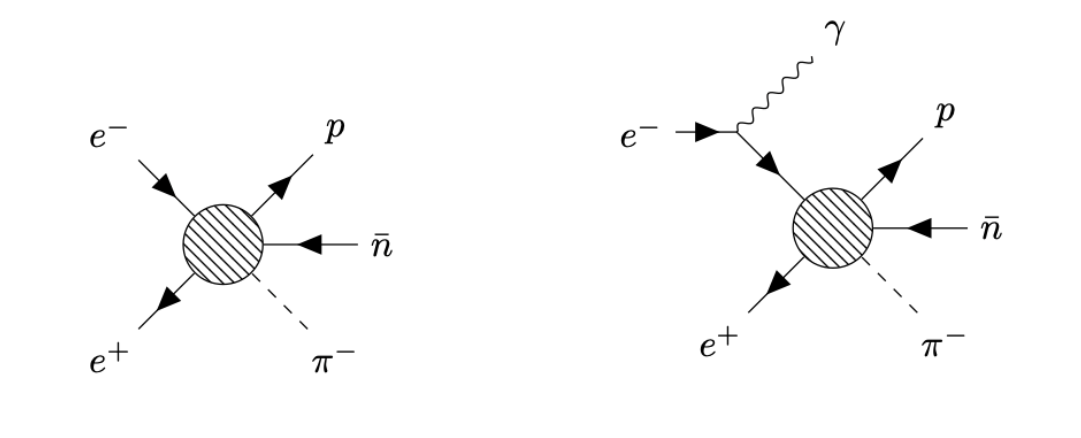
\includegraphics[width=1\textwidth]{nbar_MC/images/channel_art}
    \caption{Feynman Diagram of the channel of interest. The ISR gamma is a pre-interaction radiation emitted by the $e^+$ and/or $e^-$. The recoil system is made of $p \pi^- (\gamma_{ISR})$.}
    \label{fig:diag_F}
\end{figure}

In particular, the kinematic relation between the $\bar{n}$ and the recoil system $p \pi^- (\gamma_{ISR})$ will be exploited, considering both configurations: in the presence of Initial State Radiation (ISR) photon emission and in its absence. ISR corresponds to the emission of photons from incoming particles before they collide in high-energy physics experiments. This reduces the effective center-of-mass energy available, which will no longer be $\sim 10.58$ GeV, in the Belle II case. The ISR energy and angle distributions will be discussed in detail, providing a comparison with a simple phase space model emission.
$\\$
Then, the effect of a one constraint (1C) kinematic fit over the recoil mass will be discussed, in order to obtain a higher recoil momentum resolution.
$\\$
In total, 100000 events are generated and to perform the event generation and the analysis,  \textbf{basf2} is employed. Script code highlights for this section are shown in Appendix~\hyperref[app:A]{\ref*{app:A}}, where the decay file, MC generation file, and steering file are explained in detail.
$\\$
The basf2 \textbf{Phokhara\_evtgen\_combination} generator has been adopted. It is made of two generators: \textbf{Phokhara} and \textbf{EvtGen}.
$\\$
Phokhara is a Monte Carlo event generator that simulates $e^+e^-$ annihilation into hadrons at next-to-leading order (NLO) accuracy. This includes virtual and soft photon corrections to single-photon events, plus double hard photon emission. 
$\\$
EvtGen is a Monte Carlo event generator that simulates decays of heavy-flavor particles, primarily B and D mesons. It includes decay models for intermediate and final states with scalar, vector, and tensor mesons/resonances, as well as leptons, photons, and baryons. Decay amplitudes generate each branch of the full decay tree, accounting for angular and time-dependent correlations to simulate CP-violating processes.
$\\$
Therefore, these two generators have been adopted as depicted in Fig.~\ref{fig:diag_F_colors}.

\begin{figure}[H]
    \centering
    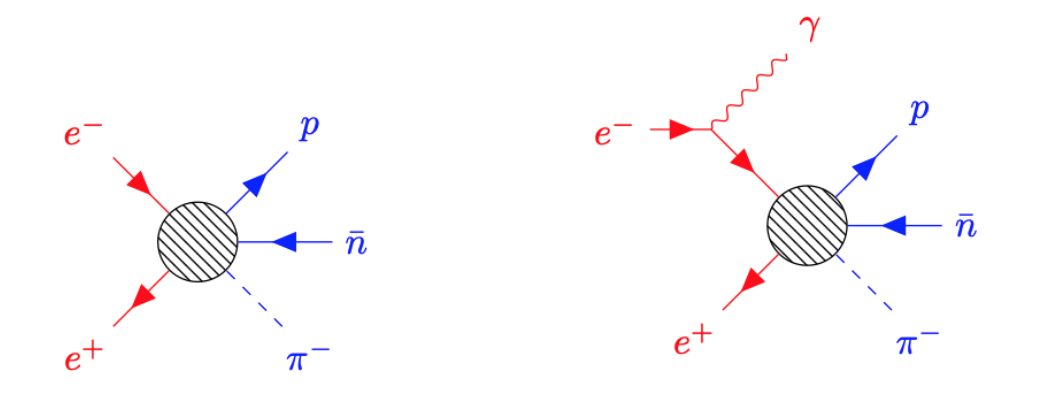
\includegraphics[width=1\textwidth]{nbar_MC/images/channel_art_colors}
    \caption{Feynman diagram of the channel of interest. \textit{Phokhara} handles the initial hard photon emission (red), while \textit{EvtGen} simulates the decay to final-state particles (blue).}
    \label{fig:diag_F_colors}
\end{figure}
Importantly, the Phokhara\_evtgen\_combination generator produces both events with and without ISR emission, as explicitly illustrated by the TopoAna overview of generated events in Fig.~\ref{fig:topo_signal0}.
$\\$
A $vpho$ (virtual photon) is now introduced as a fictitious particle used by the generator Phokhara to produce ISR photons before the $e^+ e^-$ collisions and then enforce (evt\_gen) the selected decay channel, approaching the following scheme:

\begin{center}
$e^+ \ + \  e^- \rightarrow vpho +  \ \gamma_{ISR} $ (Phokhara generator)

\vspace{0.3cm}

$vpho \rightarrow p \ + \ \pi^- \ + \ \bar{n} $ (EvtGen generator)
\end{center}
Figuratively, it can be represented as the blob shown in the Feynman diagram.

\subsection{Kinematic variables comparison}
Two scenarios can be studied. If the reconstructed final state particles are a proton ($p$), a negative pion ($\pi^-$) and an anti-neutron ($\bar{n}$), it is referred to as the \textbf{NO ISR case}. If the ISR photon ($\gamma_\text{ISR}$) is also reconstructed, it is referred to as the \textbf{ISR case}. Therefore, in the NO ISR case, the recoil system is defined as the $p\pi^-$ system, while in the ISR case it is defined as the $p\pi^-\gamma_\text{ISR}$ system. 

\begin{figure}[H]
    \centering
    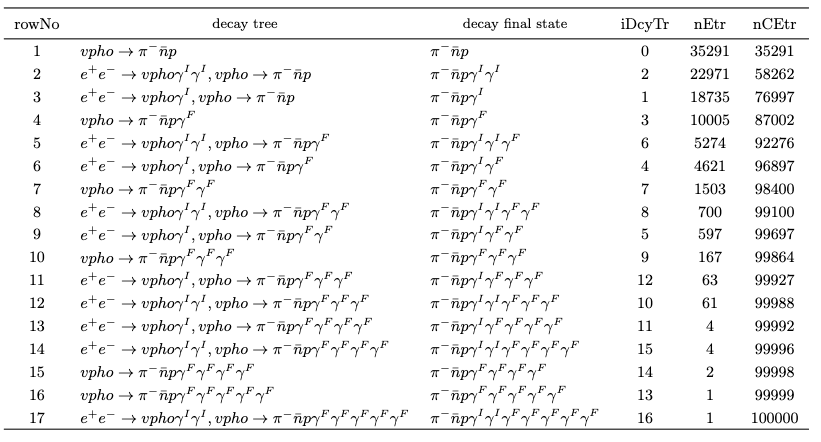
\includegraphics[width=1\textwidth]{nbar_MC/images/topoana_100k}
    \caption{Topology Analysis (TopoAna) output of the generated 100k events. The fourth column is the unambiguous decay tree index associated to the correspondent channel, the fifth the number of entries per channel, and the last the cumulative number of entries.}
    \label{fig:topo_signal0}
\end{figure}

As a first step, the kinematic variables are discussed through the recoil system consisting of $p \pi^- (\gamma_{ISR})$, where these particles are reconstructed. In parallel, the neutral $\bar{n}$ cluster candidate is reconstructed and its properties are compared to those from the recoil, comparing different kinematic variables. Through the recoil analysis, the antineutron can be identified as the missing particle in the final state.
$\\$
The first three contributes in Fig.~\ref{fig:topo_signal0} shows that events without ISR emission are the most frequently generated ($\sim 35\%$), followed by those with two ($\gamma^I\gamma^I$) ($\sim 23\%$) and one ($\gamma^I$) ISR photon ($\sim 19\%$). 
$\\$
Additionally, numerous Final State Radiation (FSR) photons are emitted by the charged final state particles due to next order perturbative QED processes.

\subsubsection{ISR distributions}
The ISR energy and angular distributions are discussed below. The primary effect of ISR emission is the reduction of the center-of-mass energy $\sqrt{s}$ below the $\Upsilon(4S)$ resonance.
$\\$
Therefore, the energy E and $\theta$ distributions of ISR radiation are shown if Fig.~\ref{fig:isr_distro}.
\begin{figure}[H]
    \centering
    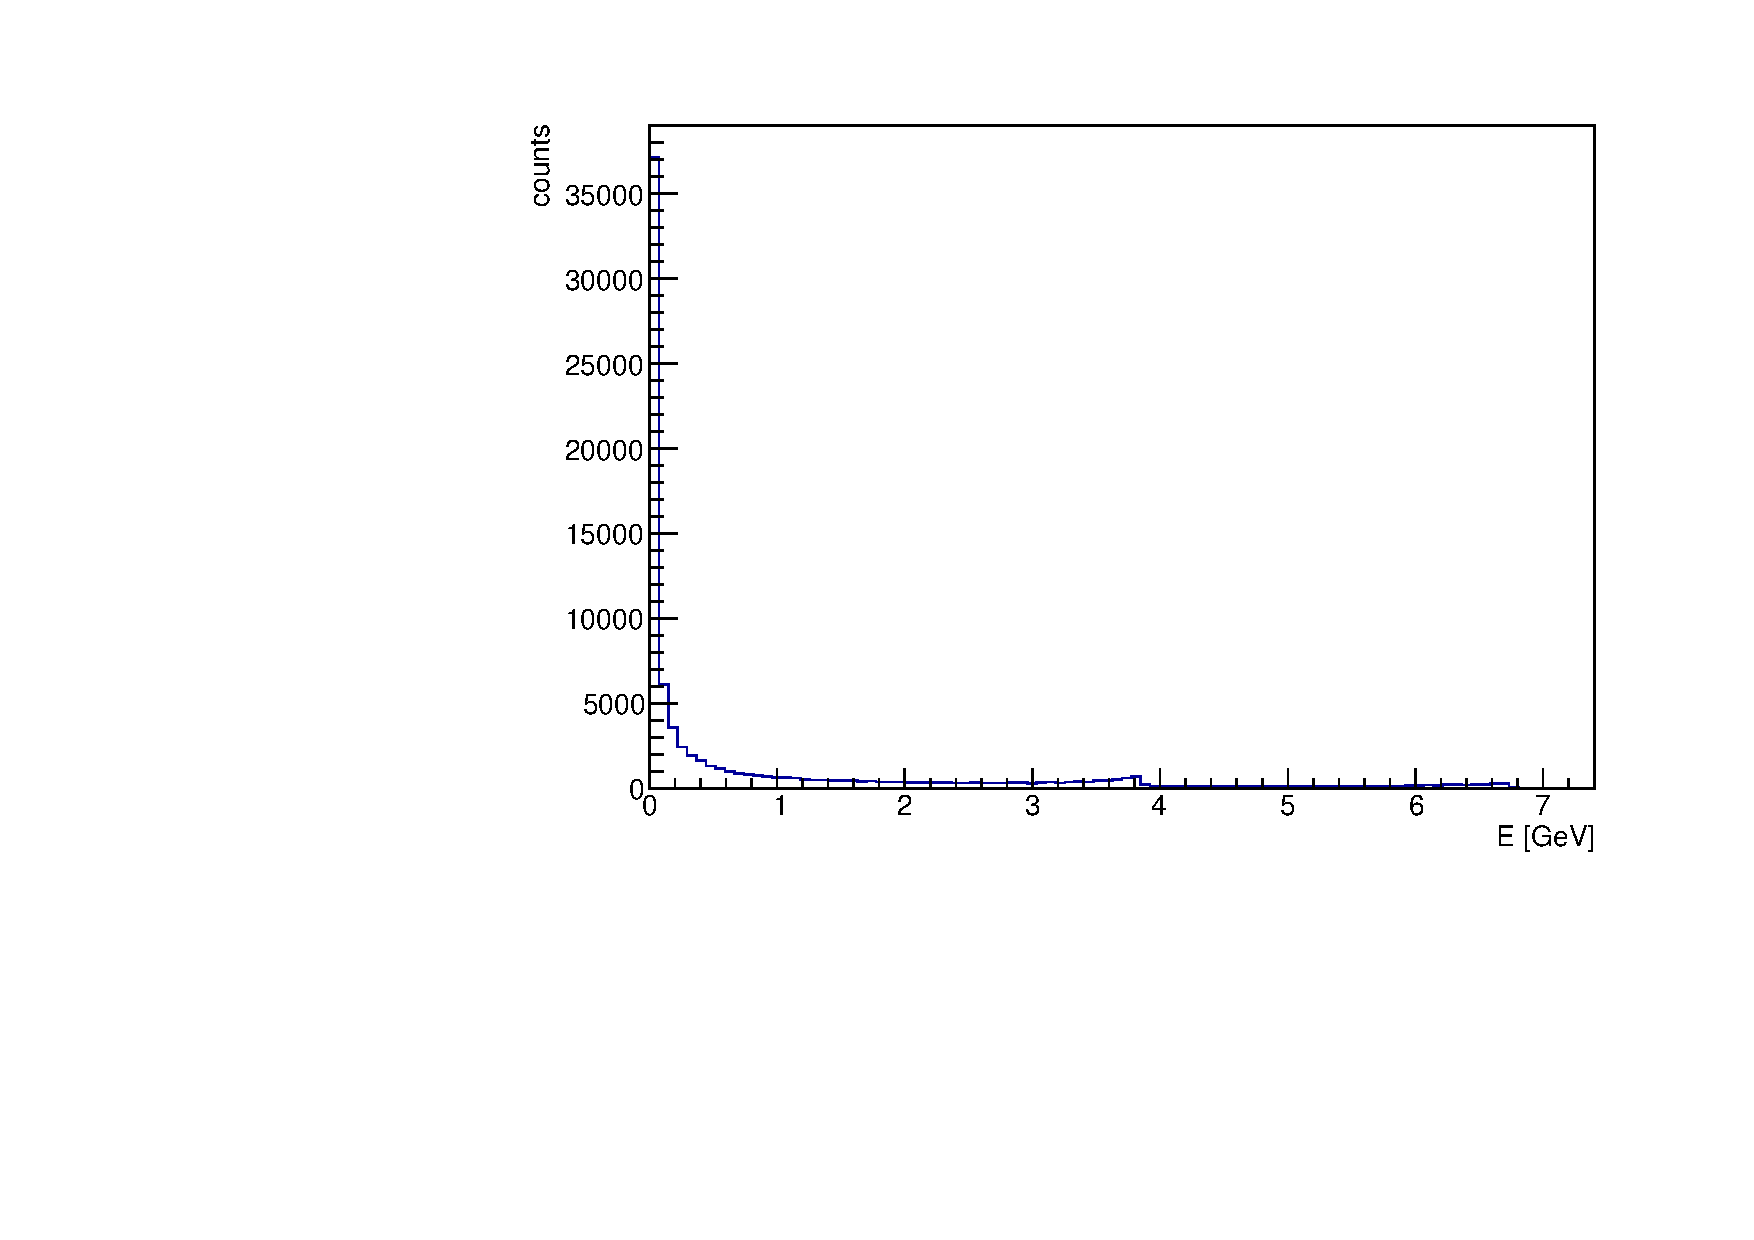
\includegraphics[width=0.49\textwidth]{nbar_MC/images/ISR_energy.pdf}
    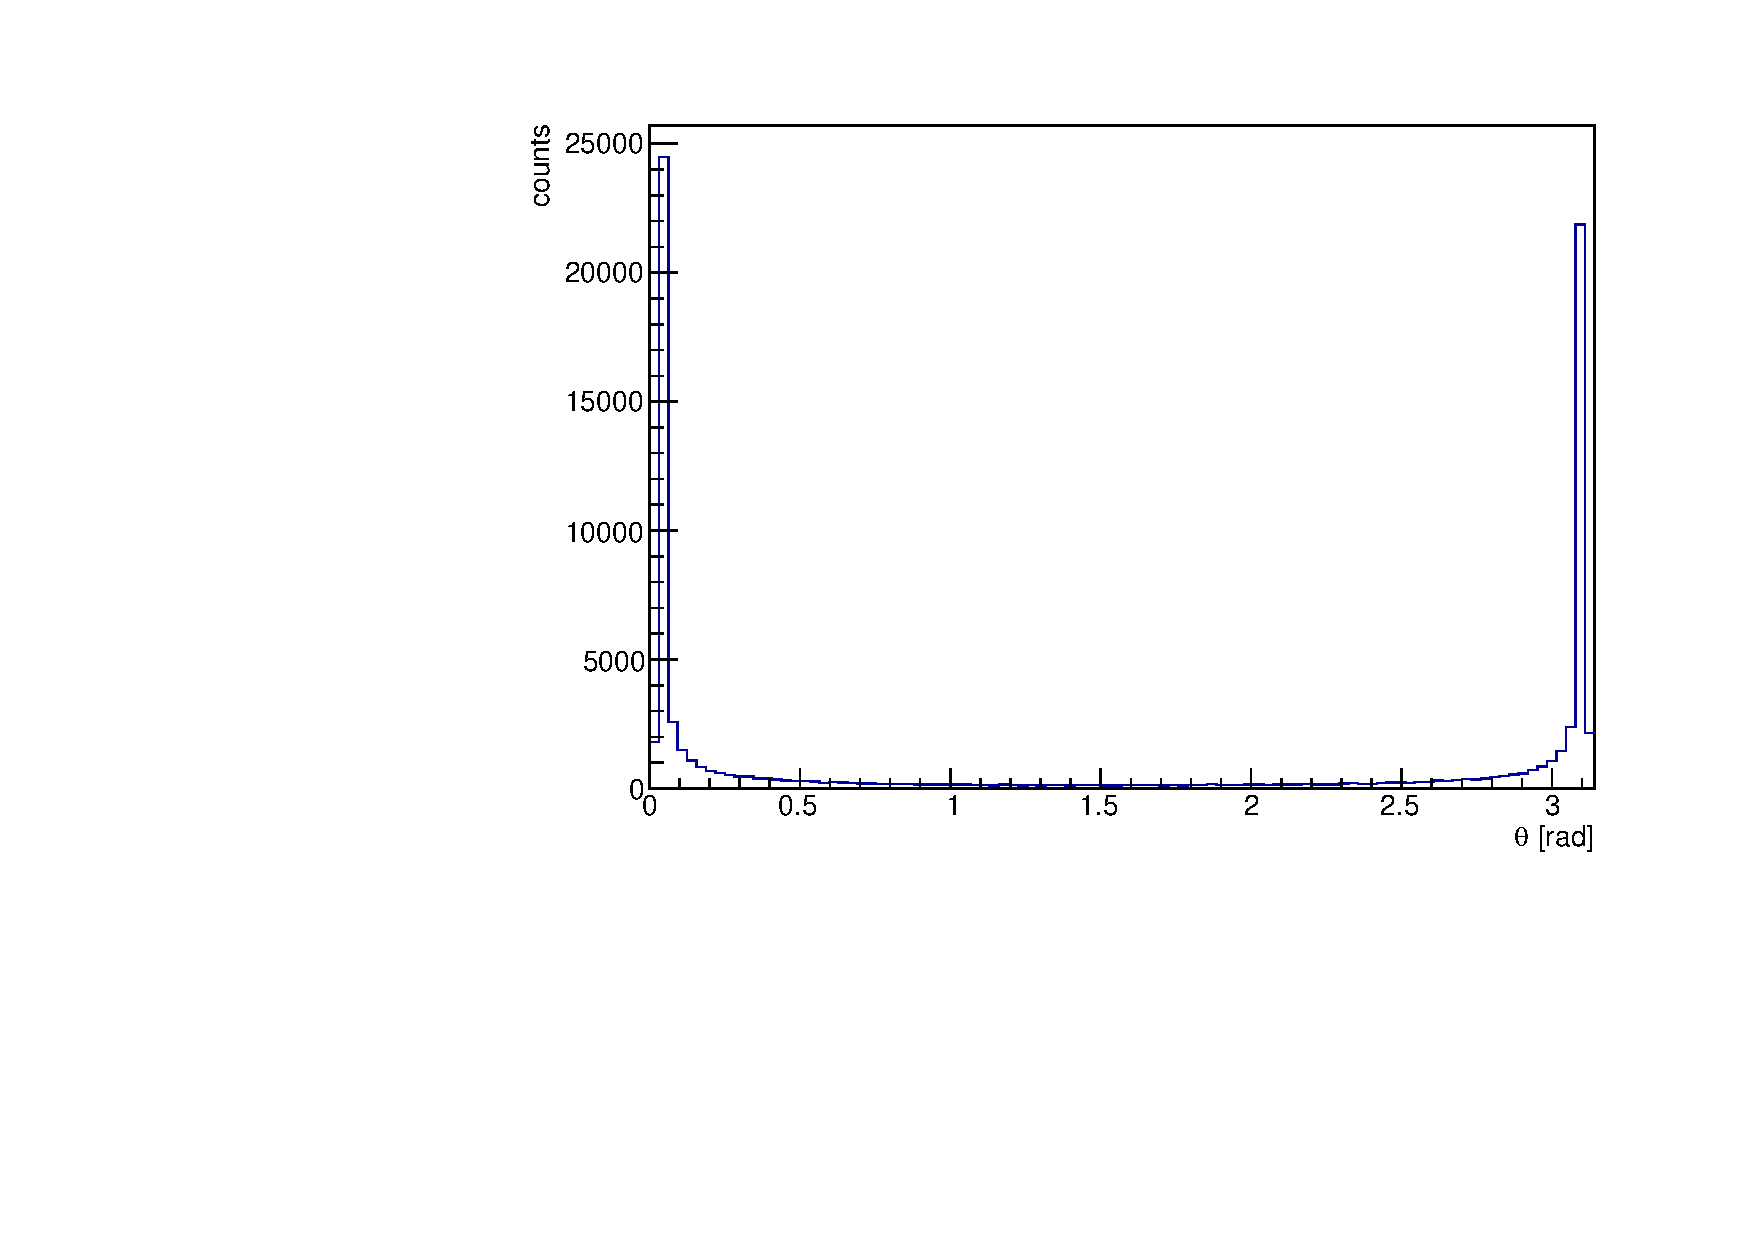
\includegraphics[width=0.49\textwidth]{nbar_MC/images/ISR_theta.pdf}
    \caption{(a) ISR energy distribution. (b) ISR $\theta$ distribution. Both distributions are shown on a logarithmic $y$-axis scale.}
    \label{fig:isr_distro}
\end{figure}

The conjugate energy E and $\theta$ distribution of ISR radiation are shown if Fig.~\ref{fig:isr_distro_conj}.
\begin{figure}[H]
    \centering
    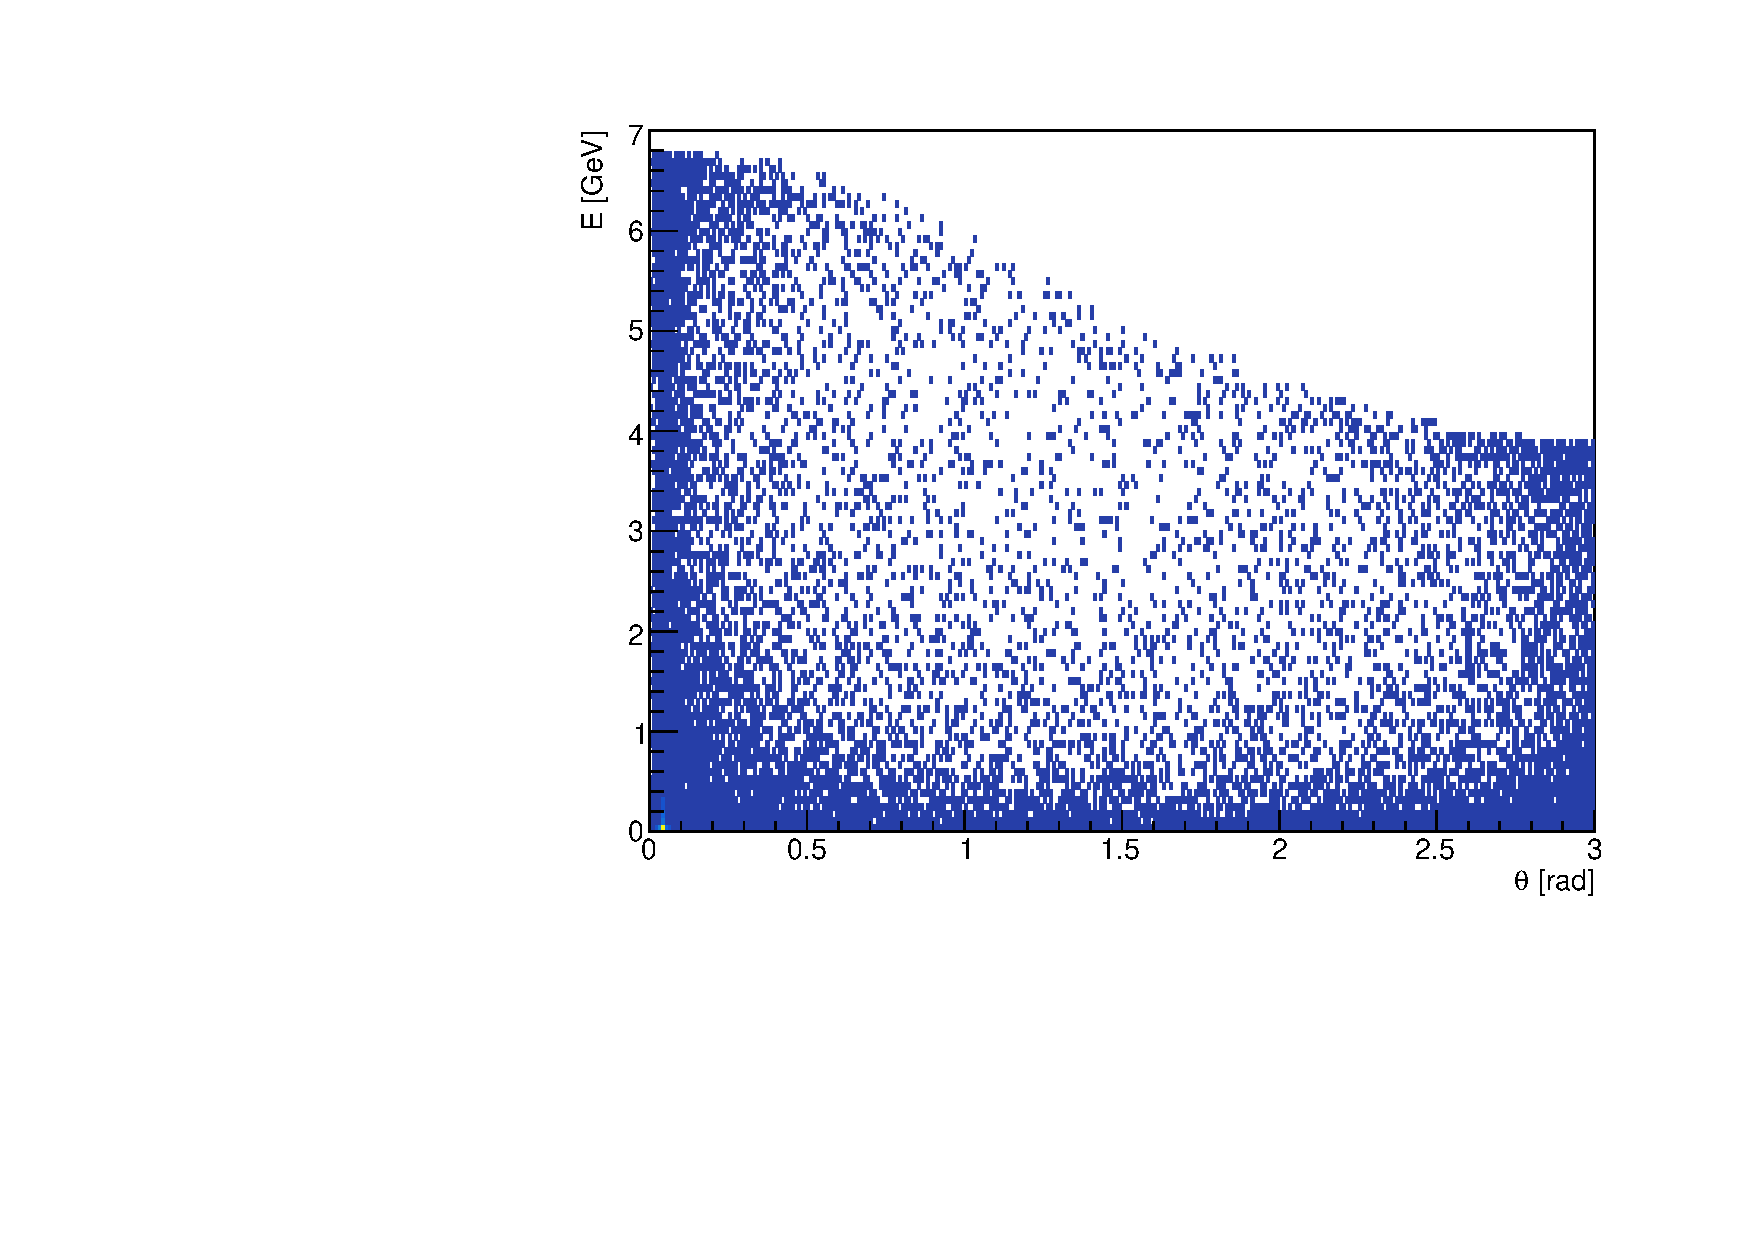
\includegraphics[width=0.70\textwidth]{nbar_MC/images/ISR_energy_vs_theta.pdf}
    \caption{Conjugate energy E and $\theta$ distribution of ISR radiation.}
    \label{fig:isr_distro_conj}
\end{figure}

The ISR energy distribution mainly consists of photons in the $[0,1]$ GeV energy. Two peaks are observed slightly below 4 GeV and 7 GeV, corresponding to the energies of the $e^+$ and $e^-$ beams, respectively. The angular distribution present a U-shape, indicating that forward and backward directions are the most probable. 
$\\$
Furthermore, as can be observed in Fig.~\ref{fig:isr_distro_conj}, the higher the energy of the ISR radiation, the closer $|cos(\theta)|$ is to 1, indicating that high-energy $\gamma_{ISR}$ photons are emitted preferentially in the forward and backward directions. The peak at low $\theta$ values (forward direction) is higher than the backward peak, consistent with the detector asymmetry with respect to the interaction point.

\subsubsection{Event selections}
In the ISR case, the final state $p\pi^-\bar{n}\gamma_\text{ISR}$ is reconstructed; the recoil of $p\pi^-\gamma_{ISR}$ is then built. In the NO ISR case, the final state $p\pi^-\bar{n}$ is reconstructed; the recoil of $p\pi^-$ is then built. Therefore, the $\bar{n}$ can be identified through the recoil mass peak at the anti-neutron mass. 
$\\$
To properly select the signal in the recoil mass distribution, several cuts are applied in the steering file as follows:

\begin{enumerate}
\item Recoil system: $0 \ GeV/c^2 <recoil \ mass < 2 \ GeV/c^2$
\item $\bar{n}$: neutral clusters from ECL
\item $p$: $protonID > 0.9$ and $dr<1$ cm and $|dz|<3$ cm 
\item $\pi^-$: $pionID > 0.1$ and $dr<1$ cm and $|dz|<3$ cm 
\end{enumerate}

The first one is a cut that selects the region of interest in the recoil mass distribution, corresponding to the interval [0,2] $GeV/c^2$ around the antineutron mass ($\sim 939,56$ $MeV/c^2$). 
$\\$
To analyze only $\bar{n}$ signals from the calorimeter, the second selection requires that the neutral $\bar{n}$ cluster candidates are reconstructed within the electromagnetic calorimeter (ECL), avoiding the $\bar{n}$ candidates from other detectors (mainly from KLM).
$\\$
The third and fourth criteria are standard selections recommended by the basf2 framework. The ID requirement imposes a constraint on the protonID or pionID based on a maximum likelihood criterion as follows:
\begin{center}
$protonID = \frac{L_p}{L_e + L{\mu} + L{\pi} +L_K + L_d }$
\hspace{0.3cm}
$pionID = \frac{L_\pi}{L_e + L{\mu} + L{p} +L_K + L_d }$,
\end{center}
where $L_p$ is the likelihood for the proton hypothesis, $L_{\pi}$ is the likelihood for the pion hypothesis, and so on.
$\\$
The cuts on $dr$ and $|dz|$ select only tracks originating from the interaction point (IP) area, where $dr$ is defined as the transverse distance with respect to IP and $dz$ is defined as the axial distance, along the z-axis, with respect to IP.
$\\$
Since multiple $\bar{n}$ neutral cluster candidates may exist per event, only the candidate with the smallest angle -defined as $\alpha$- relative to the recoil system is selected. Therefore, a selection is imposed using the basf2 \textbf{rankByLowest} method. It allows to select only the highest rank candidates, based on a specific variable; in this case, the angle between the neutral cluster and the recoil vector.
$\\$
Using spherical coordinate system, after some algebraic steps, the 3D angle $\alpha$ between the two vectors can be obtained:

\begin{center}
$\alpha = arcos[sin(\theta_1)sin(\theta_2)cos(\phi_1 - \phi_2) + cos(\theta_1)cos(\theta_2) ]$
\end{center}

Here vector \textbf{1} denotes the recoil vector and the vector \textbf{2} denotes the $\bar{n}$ direction vector. The respective $\alpha$ distributions, before and after the aforementioned selection, are shown in Fig.~\ref{fig:alpha_pre_post}, in both ISR and NO ISR cases:

\begin{figure}[H]
    \centering
    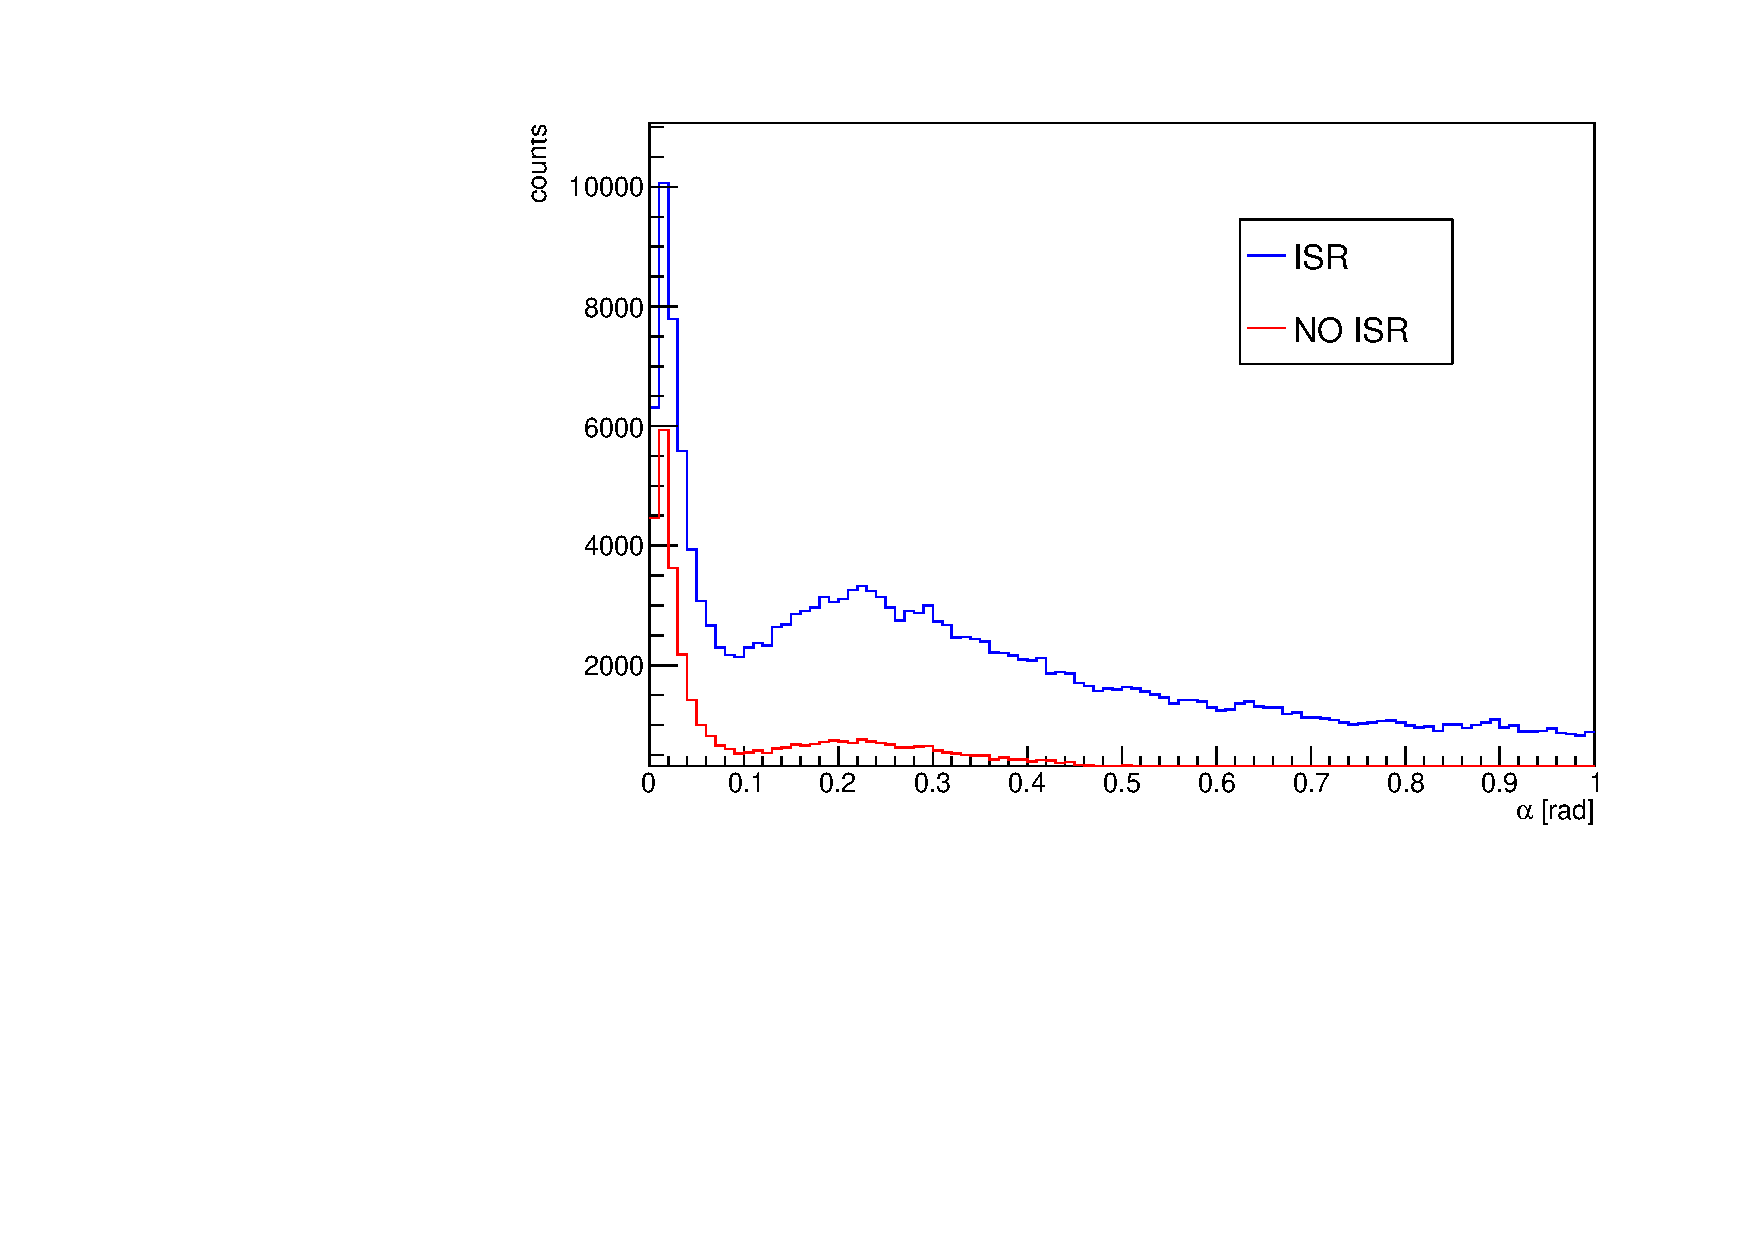
\includegraphics[width=0.49\textwidth]{nbar_MC/images/alpha_uncorr.pdf}
    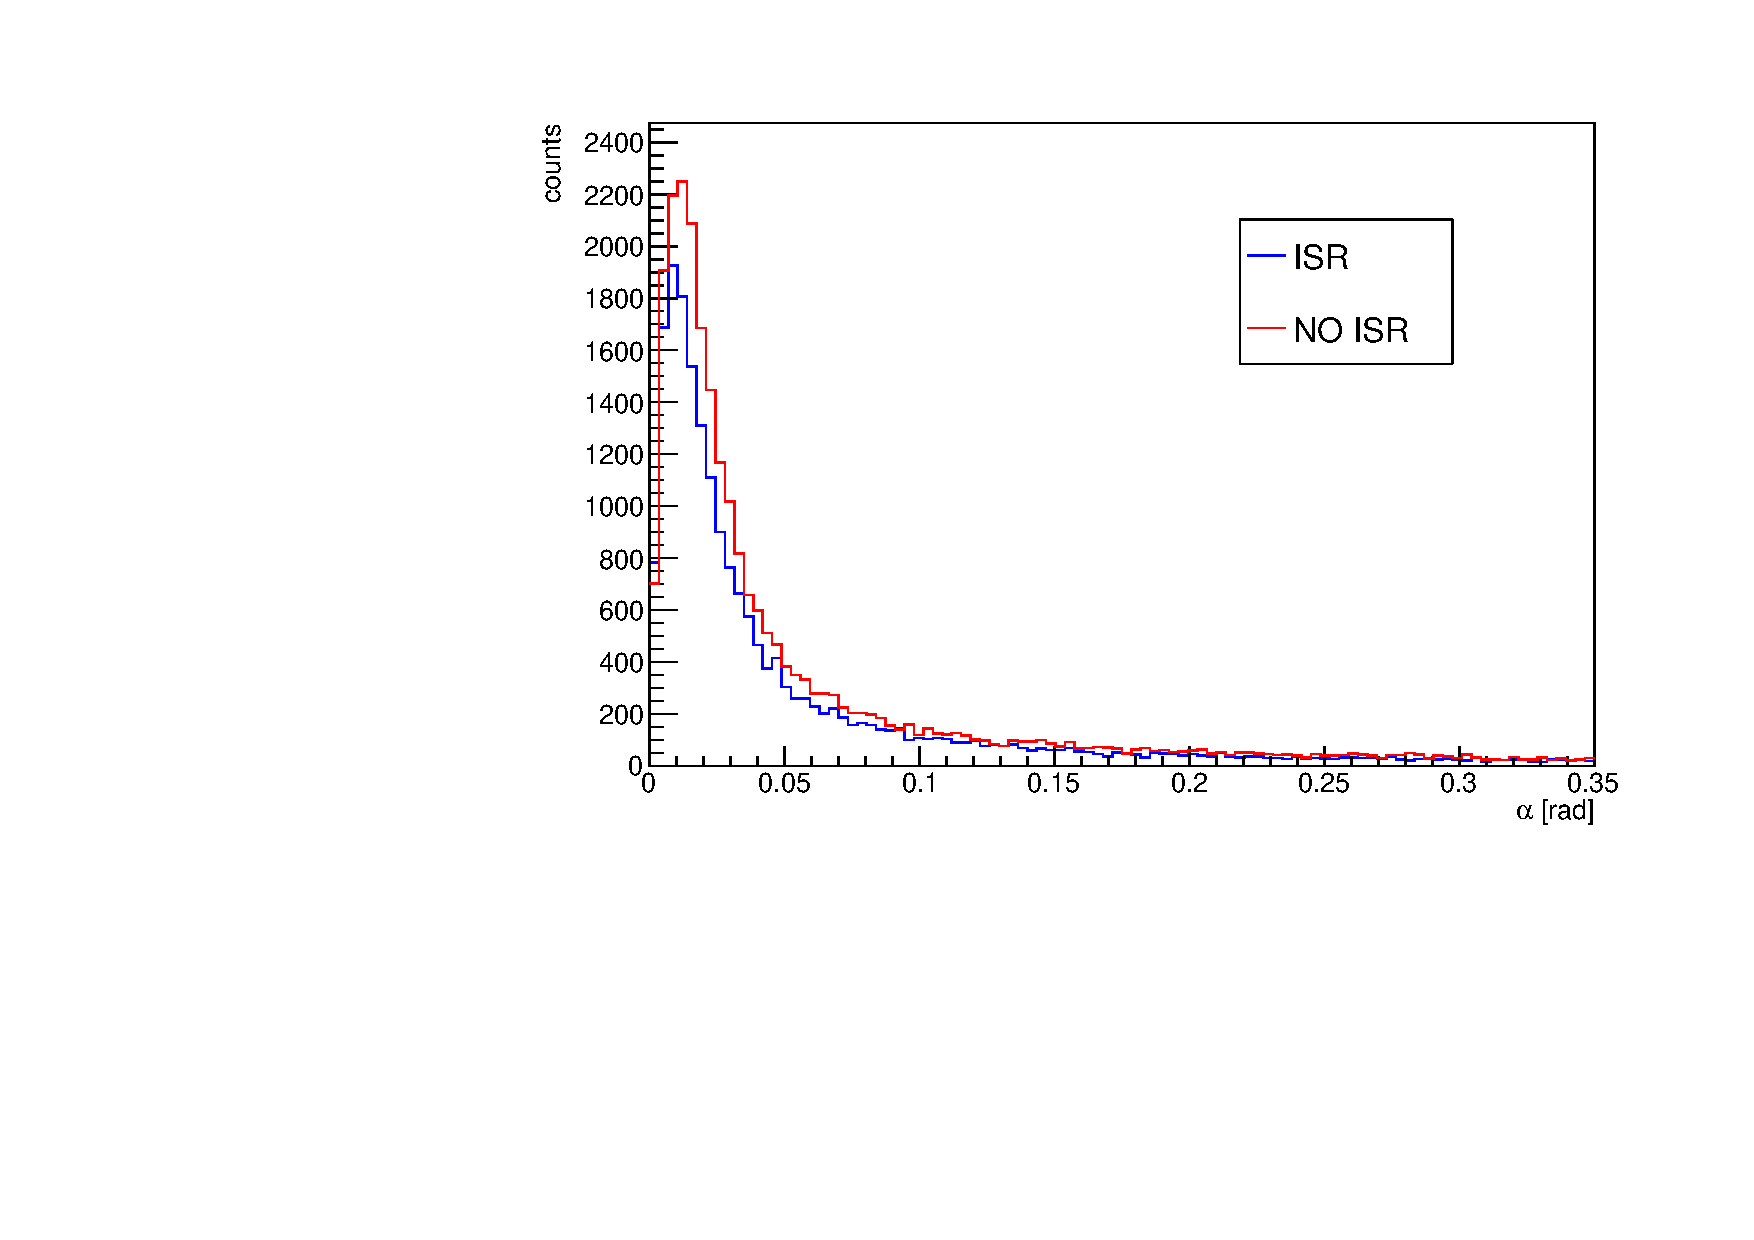
\includegraphics[width=0.49\textwidth]{nbar_MC/images/alpha.pdf}
    \caption{(a) $\alpha$ distribution. (b) $\alpha$ distribution after the rank selection.}
    \label{fig:alpha_pre_post}
\end{figure}

To select the most probable $\bar{n}$ candidates, only those with $\alpha < 0.35$ ($\sim 20^\circ$) are stored.
$\\$
The efficiency $\epsilon$  is defined as follows:
\begin{center}
  $\epsilon = \frac{n^{\circ} \ of \ reconstructed \ candidates}{n^{\circ}  \ of \ generated \ events} $
\end{center}

Referring to Fig.~\ref{fig:topo_signal0}, 46969 events are generated without ISR emission ($iDcyTr \in {0,3,7,9,14,13}$) and 53031 with ISR emission ($iDcyTr \in {2,1,6,4,8,5,12,10,11,15,16}$) .
$\\$
Since 20146 candidates are reconstructed for the ISR case and 25013 for the NO ISR case, an efficiency respectively of $\sim 53\%$ and $38\%$ can be observed.
Since most of the ISR radiation is emitted in the backward ($\theta \sim 180^{\circ}$) and in the forward ($\theta \sim 0^{\circ}$) directions -where detection coverage is absent- the efficiency in the ISR case is slightly lower than in the NO ISR case.

\subsubsection{Recoil mass distribution}
To select events with anti-neutron, the recoil system $p \pi^- (\gamma_{ISR})$ is studied through the recoil mass. Specifically, the recoil mass should peak at the nominal anti-neutron mass, since no background channels are present in this sample. The only background consists of secondary particles produced during the propagation of primary particles through the detectors. 
$\\$
The recoil mass distribution, for both ISR and NO ISR cases, is shown in Fig.~\ref{fig:recMass_distro_isr_noisr}.

\begin{figure}[H]
    \centering
    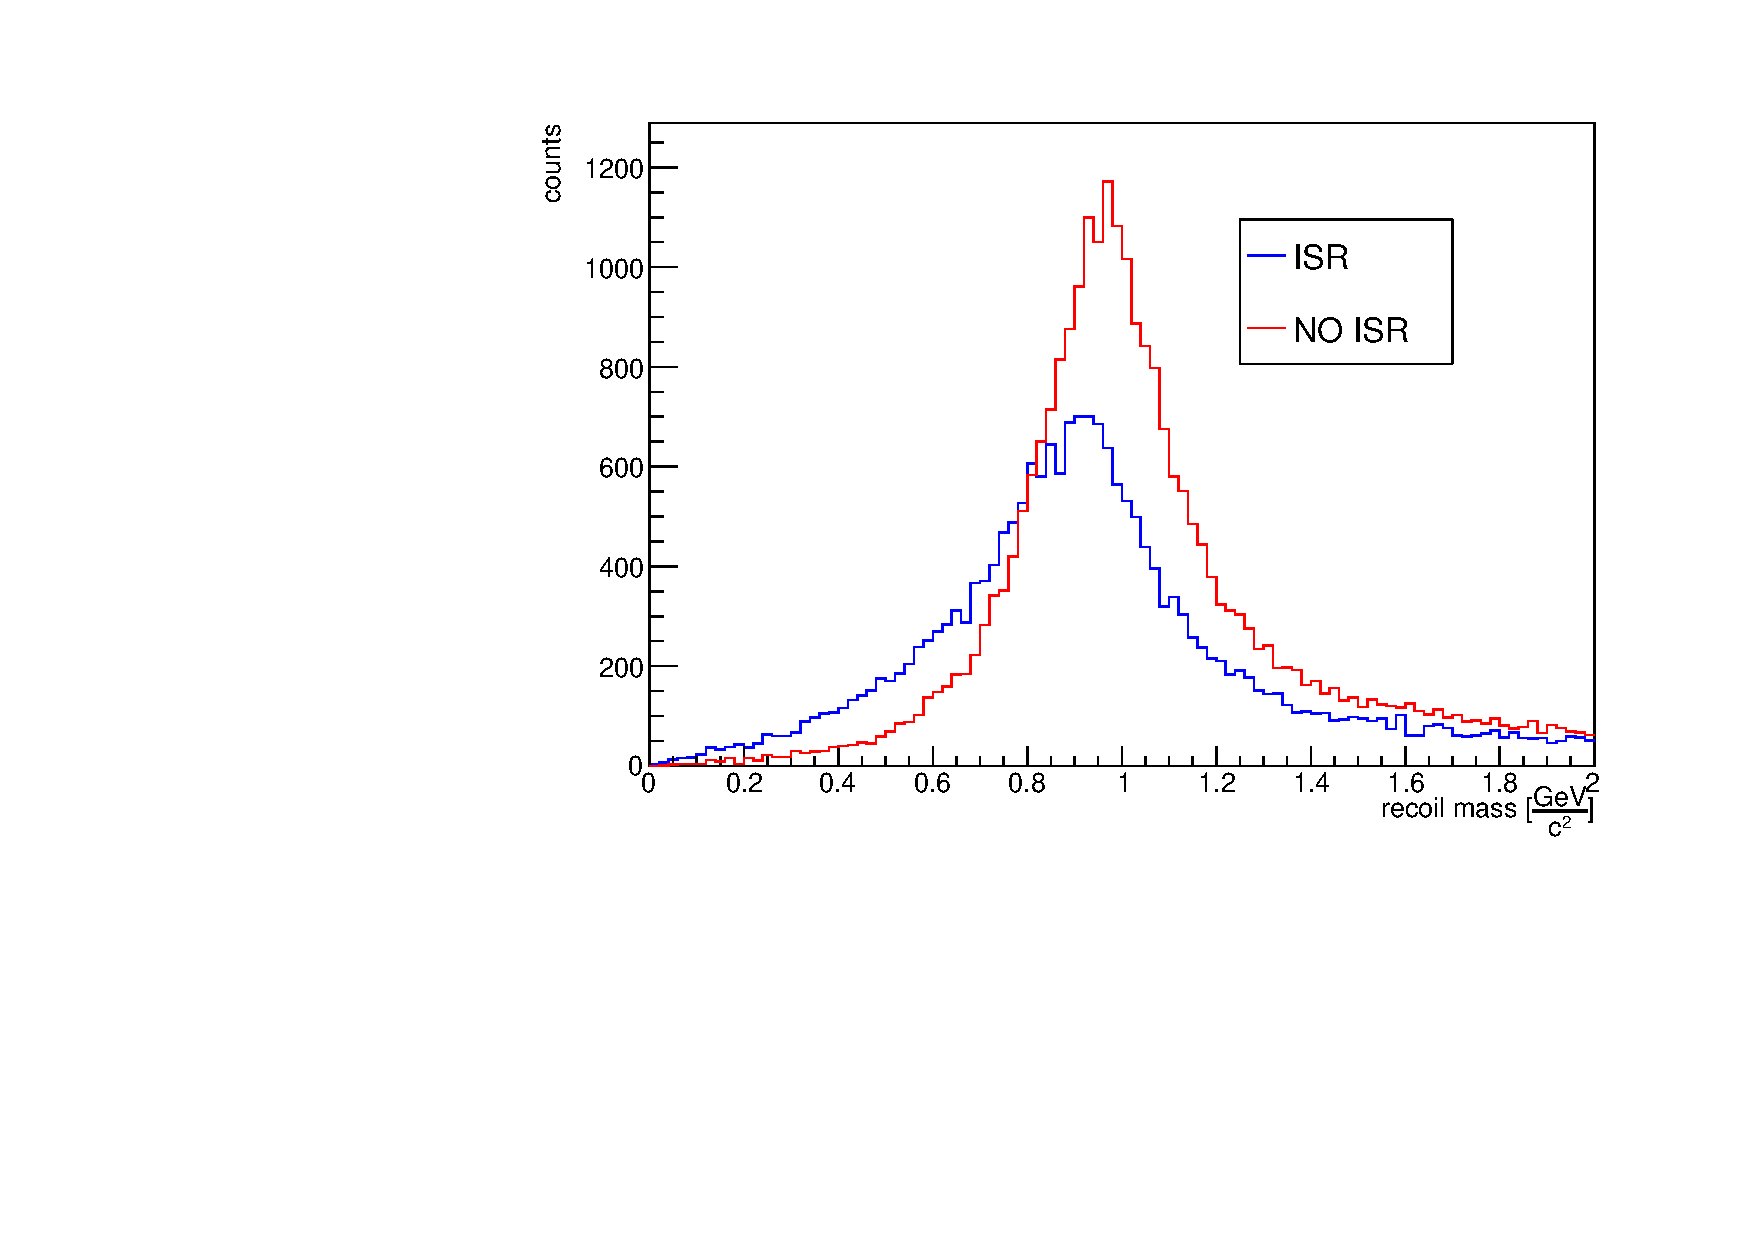
\includegraphics[width=0.7\textwidth]{nbar_MC/images/vpho_mRecoil.pdf}
    \caption{Recoil mass distribution, in both ISR and NO ISR cases.}
    \label{fig:recMass_distro_isr_noisr}
\end{figure}

The recoil mass distribution peaks on the $\bar{n}$ mass ($\sim 939.56$ MeV), indicating that the the recoil mass is well reconstructed in both ISR ($p \ \pi^-  \ \gamma_{ISR}$) and NO ISR ($p \ \pi^-$) cases. Therefore, the variables associated with the $\bar{n}$ clusters can be compared with the reconstructed recoil variables ($p, \ \theta$).
$\\$
In the event simulation the generator produces more than one $\gamma_{ISR}$ per event, reflecting into the obtained recoil mass distribution; the one obtained in ISR case shows more entries in the left tail, since only the most energetic gamma is considered in the recoil reconstruction, while the others are not considered. 
$\\$
The distribution obtained in the NO ISR case exhibits a higher peak as the recoil system reconstruction consists only of $p\pi^-$, allowing better resolution than the ISR case, since fewer tracks are considered.
$\\$
By selecting events around the peak, $\bar{n}$ candidates events can be identified. The recoil direction is expected to provide a good estimate of the $\bar{n}$ momentum.

\subsubsection{The recoil kinematic}
Before analyzing the recoil momentum distribution, the reconstructed momentum of each particle composing the recoil system is examined. For particles with MC association, the MC variables can be studied for a given list of candidates as well. 
$\\$
For example, considering the proton candidate list, both the \textbf{reconstructed} momentum of the proton list and the Monte Carlo (\textbf{generated}) momentum of the proton list -which is not affected by the reconstruction process- are available. The latter will be referred to as the "generated" momentum.
$\\$
Since a candidate list is the result of the reconstruction process, it also contains particles that have been mis-identified as the main particle (for example, $\pi^+$ mis-identified as $p$ or $\gamma$ mis-identified as $\bar{n}$).
$\\$
Therefore, the considered "generated" variables represent the Monte Carlo values for a given reconstructed particle list, which differs from the Monte Carlo values for a generator-level particle list that contains only the selected particle type.

The relative reconstructed momenta are shown in FIg.~\ref{fig:rec_p_pi_mom}.

\begin{figure}[H]
    \centering
    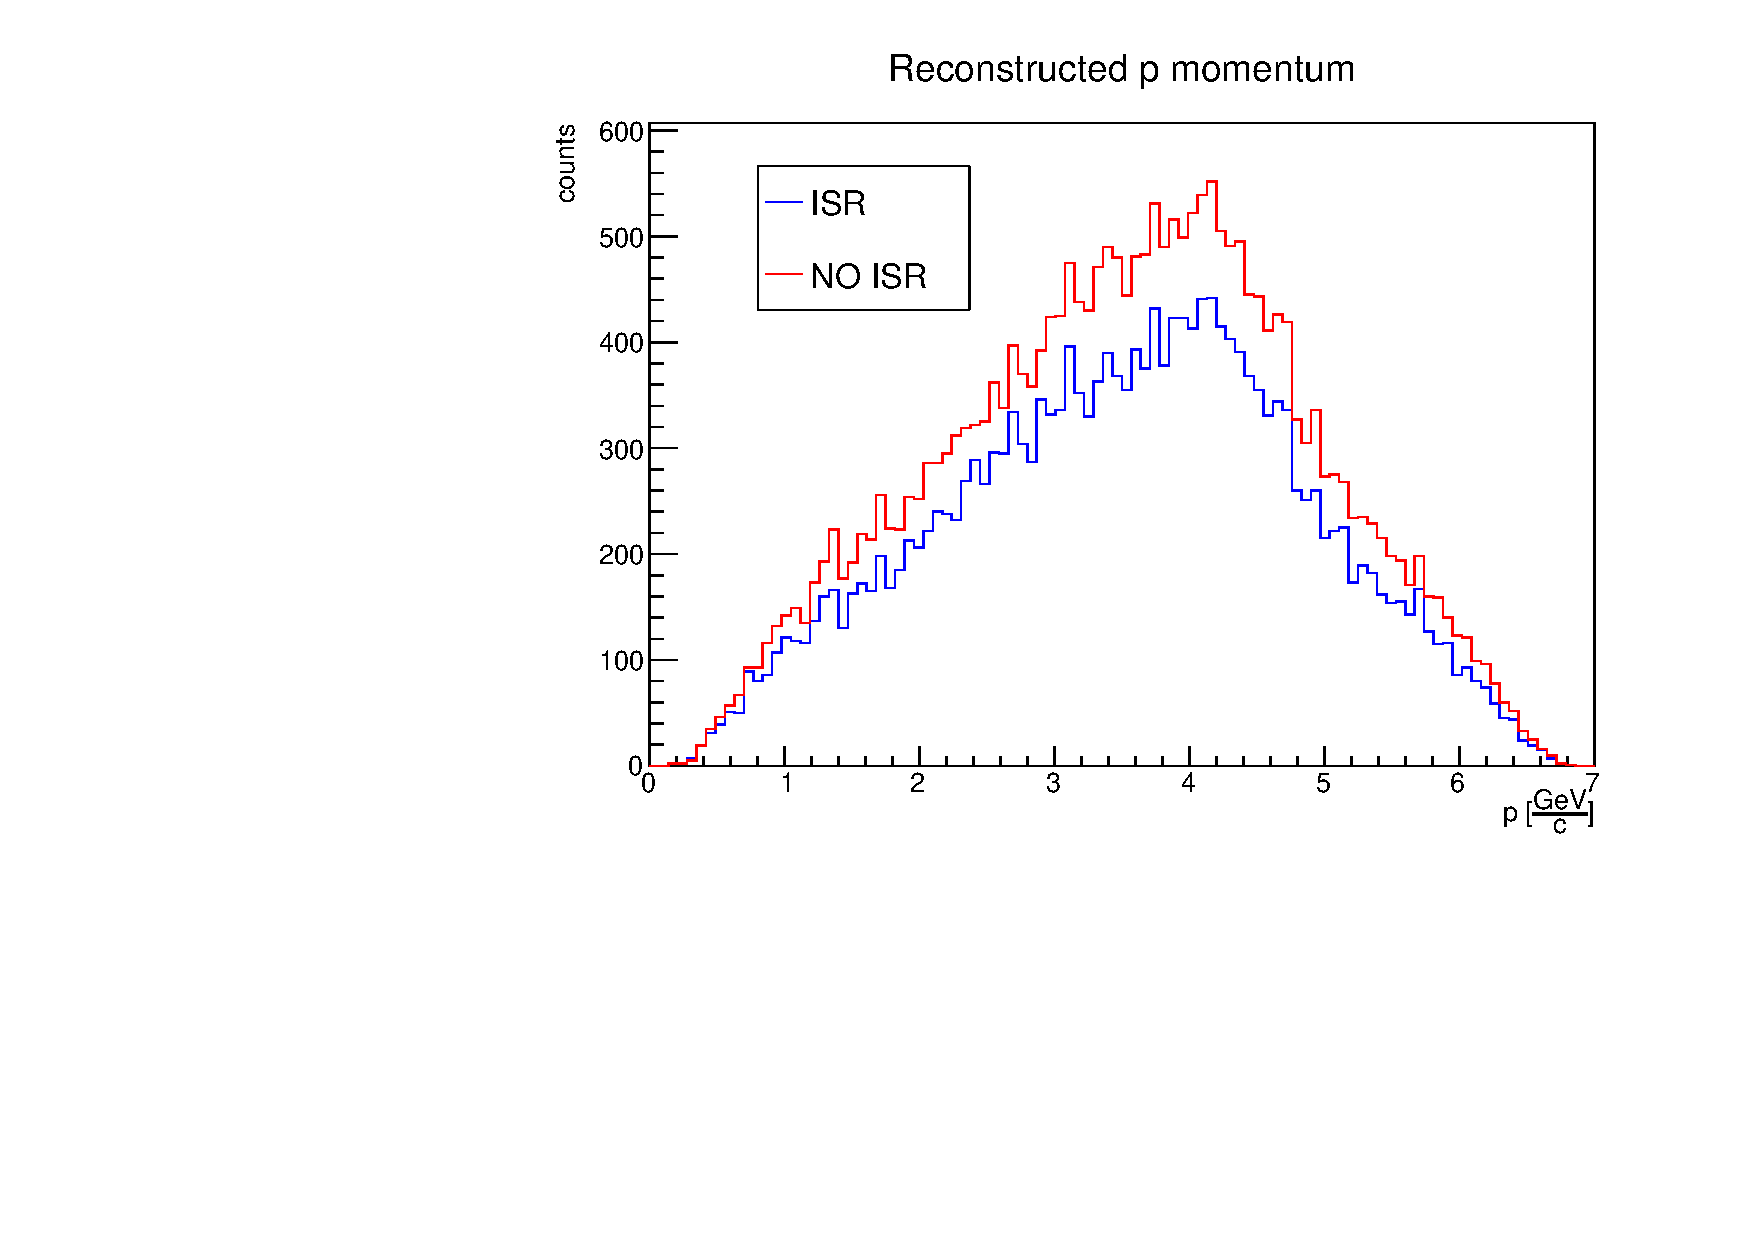
\includegraphics[width=0.49\textwidth]{nbar_MC/images/p_p.pdf}
    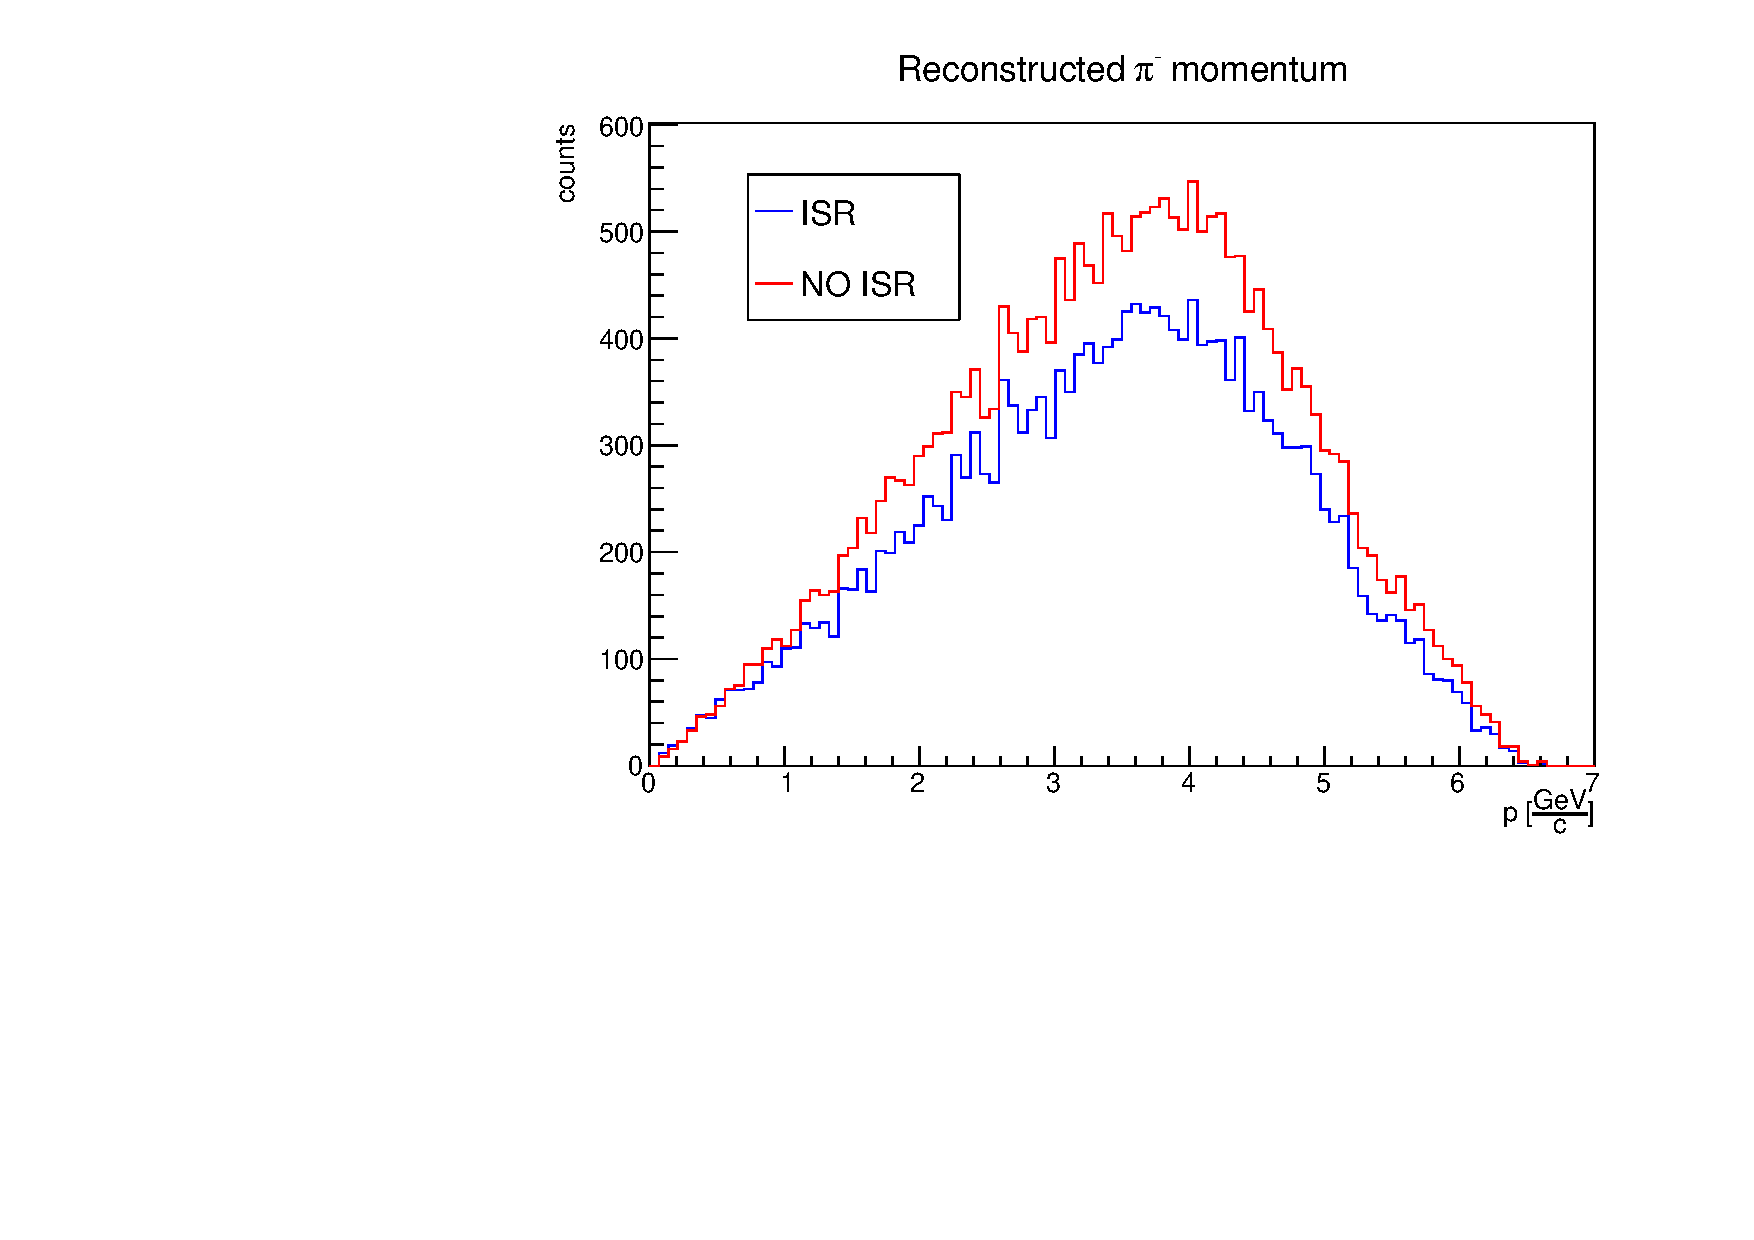
\includegraphics[width=0.49\textwidth]{nbar_MC/images/pi_p.pdf}
    \caption{Reconstructed momentum distribution of proton and pion, in both ISR and NO ISR cases}
    \label{fig:rec_p_pi_mom}
\end{figure}

The distributions clearly exhibit the typical phase-space shapes, as expected from the adopted generator model (\hyperref[app:A]{Appendix~\ref*{app:A}}). Similarly, these distributions can be obtained directly at the generator level, yielding:

\begin{figure}[H]
    \centering
    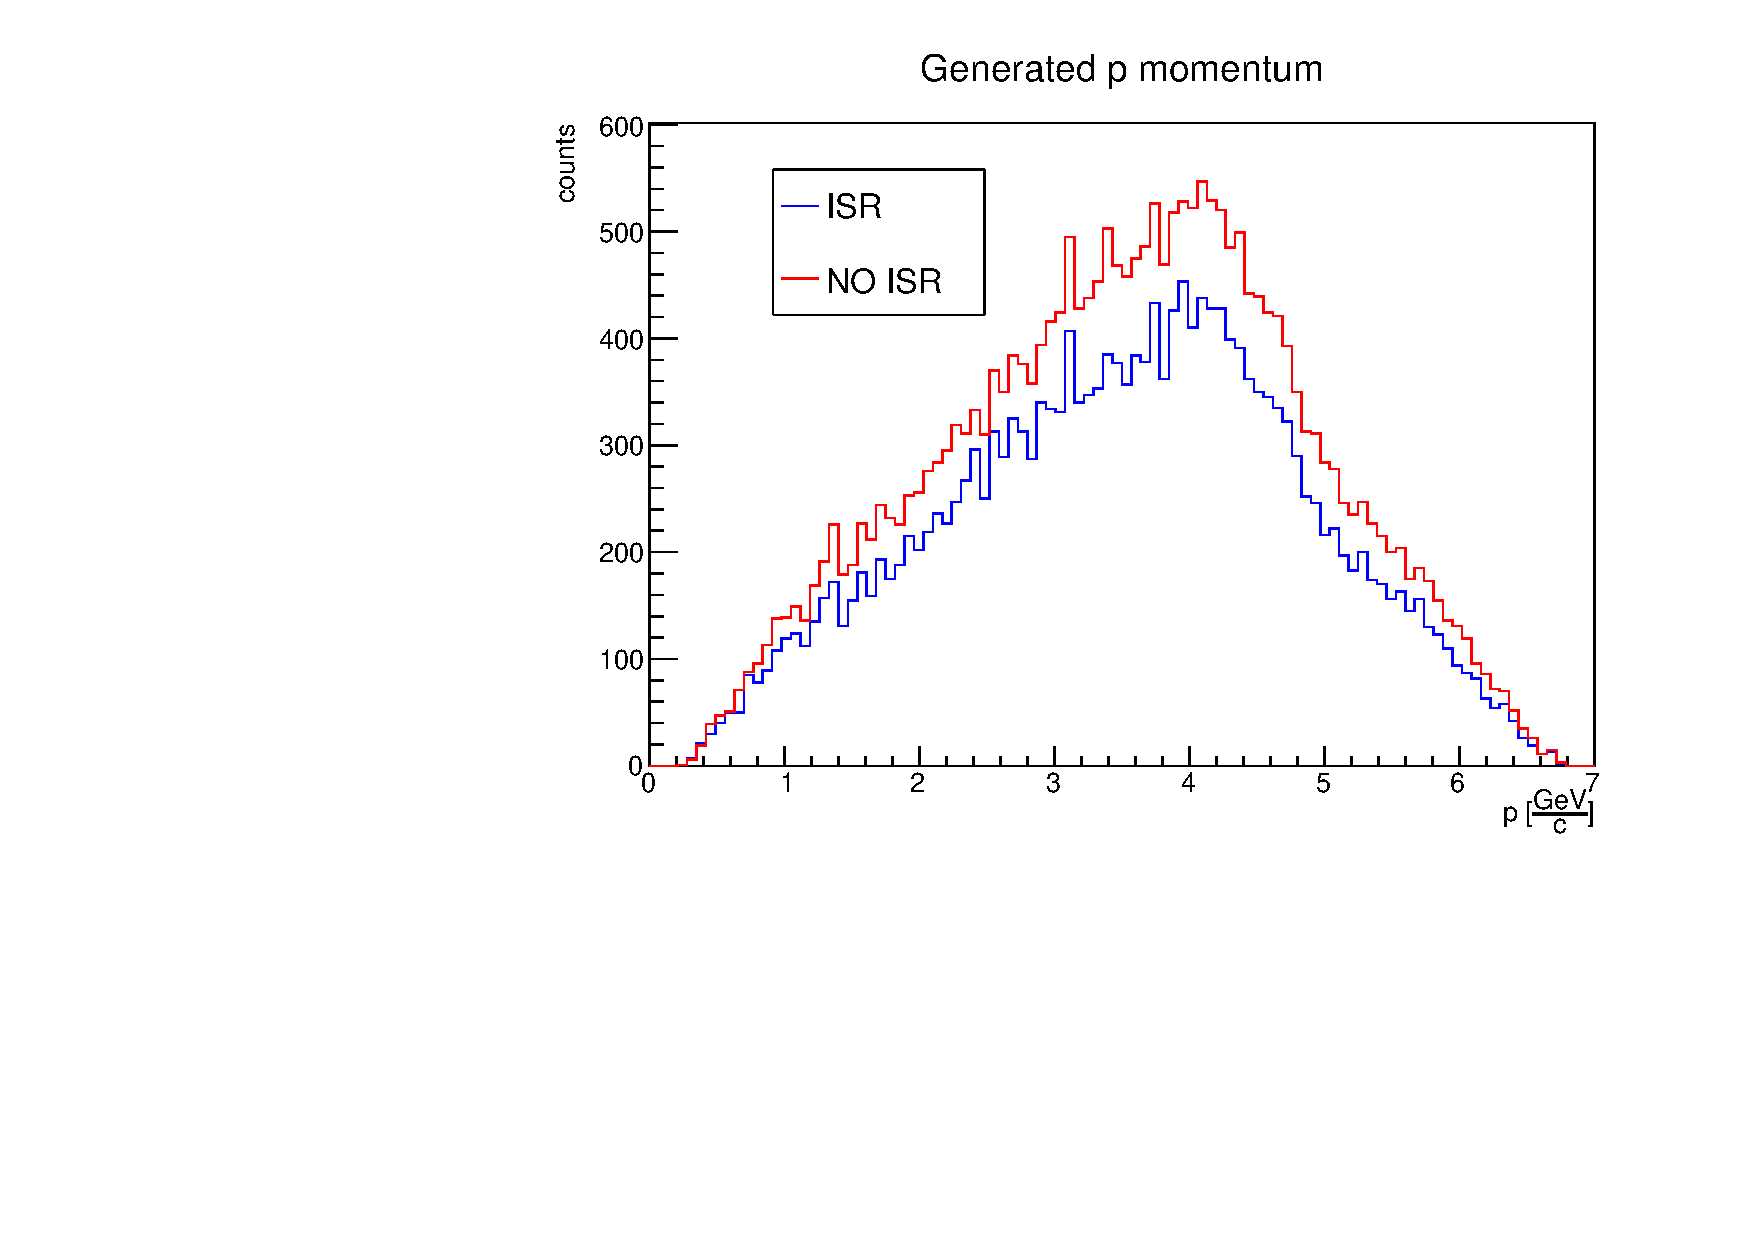
\includegraphics[width=0.49\textwidth]{nbar_MC/images/p_mcP.pdf}
    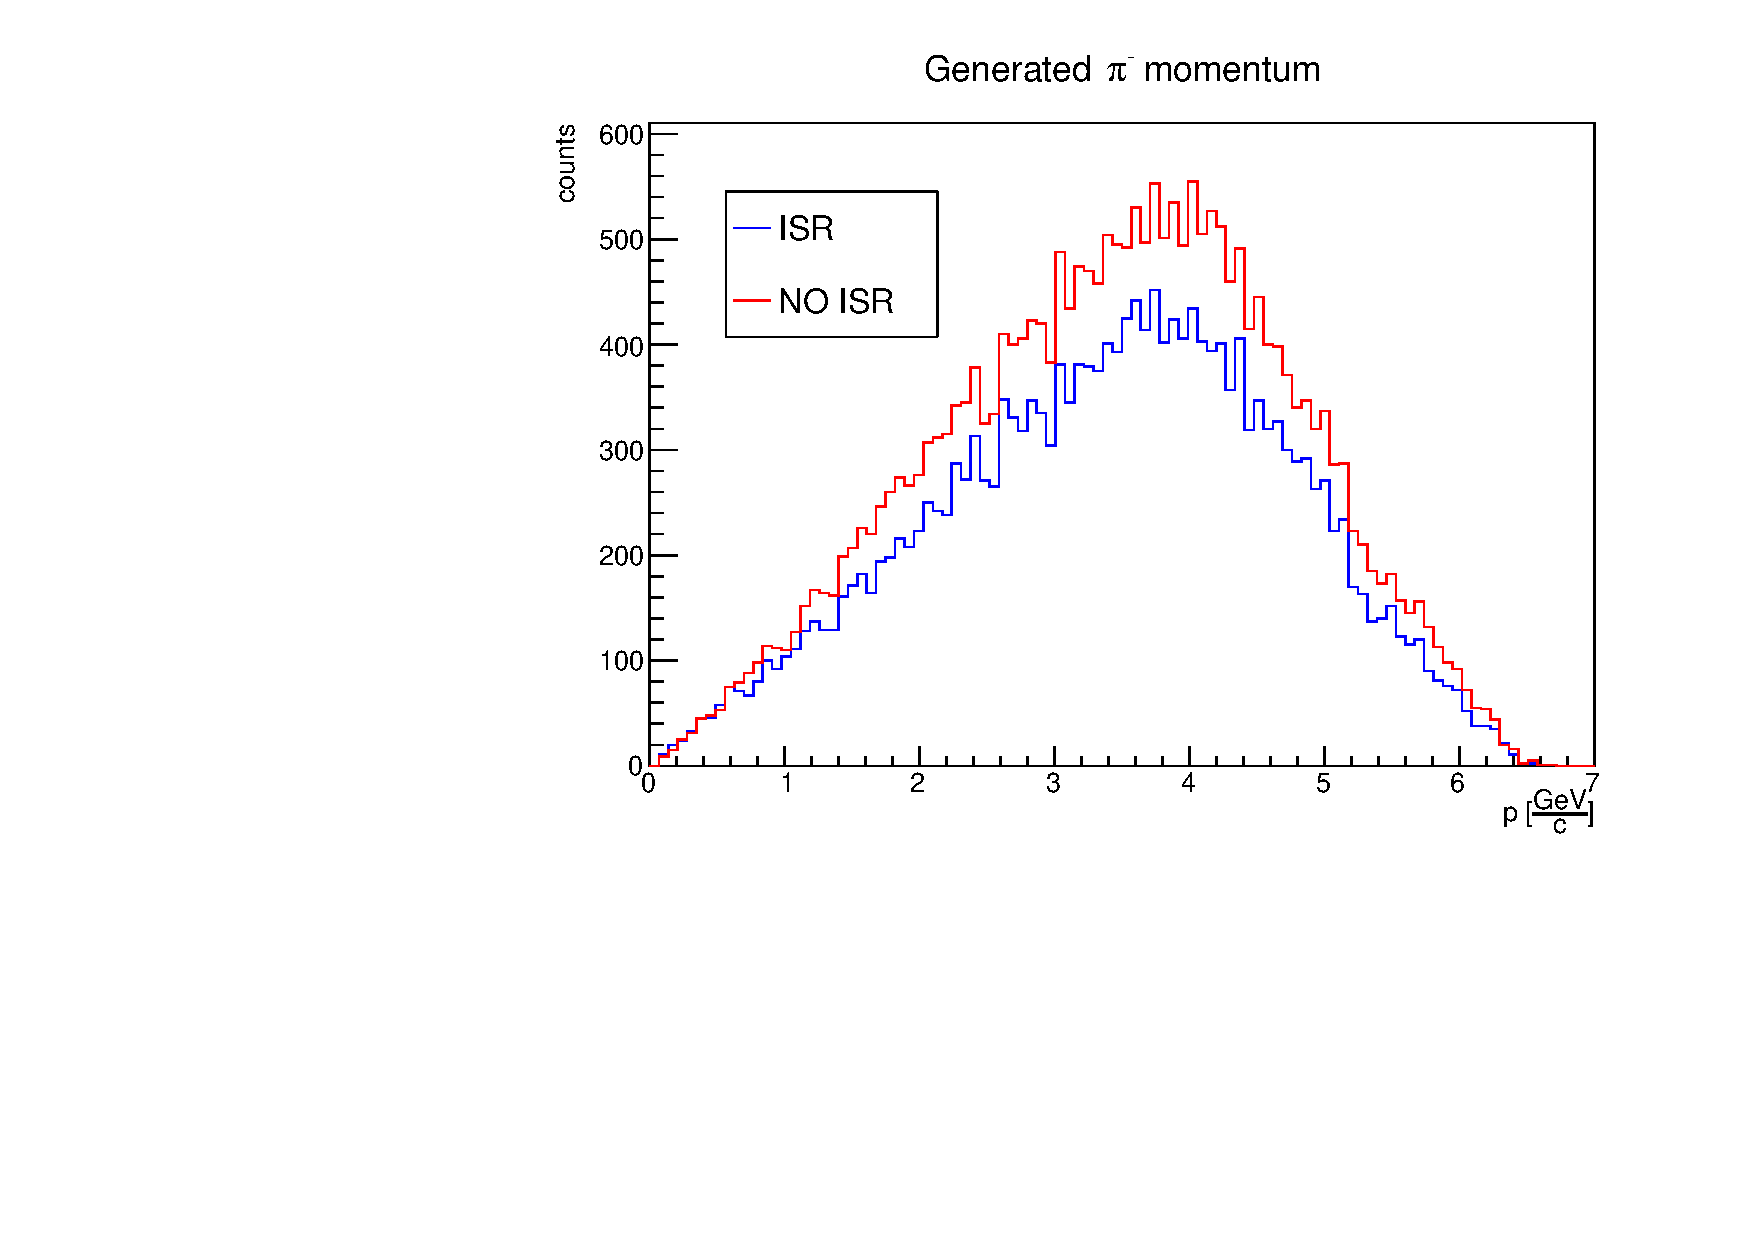
\includegraphics[width=0.49\textwidth]{nbar_MC/images/pi_mcP.pdf}
        \caption{Generated momentum distribution of proton and pion, in both ISR and NO ISR cases}
\end{figure}

Both distributions exhibit similar shapes, indicating a proper reconstruction of charged particles by the software.
$\\$
The reconstructed recoil momentum can be obtained in both ISR and NO ISR cases, as follows:

\begin{figure}[H]
    \centering
    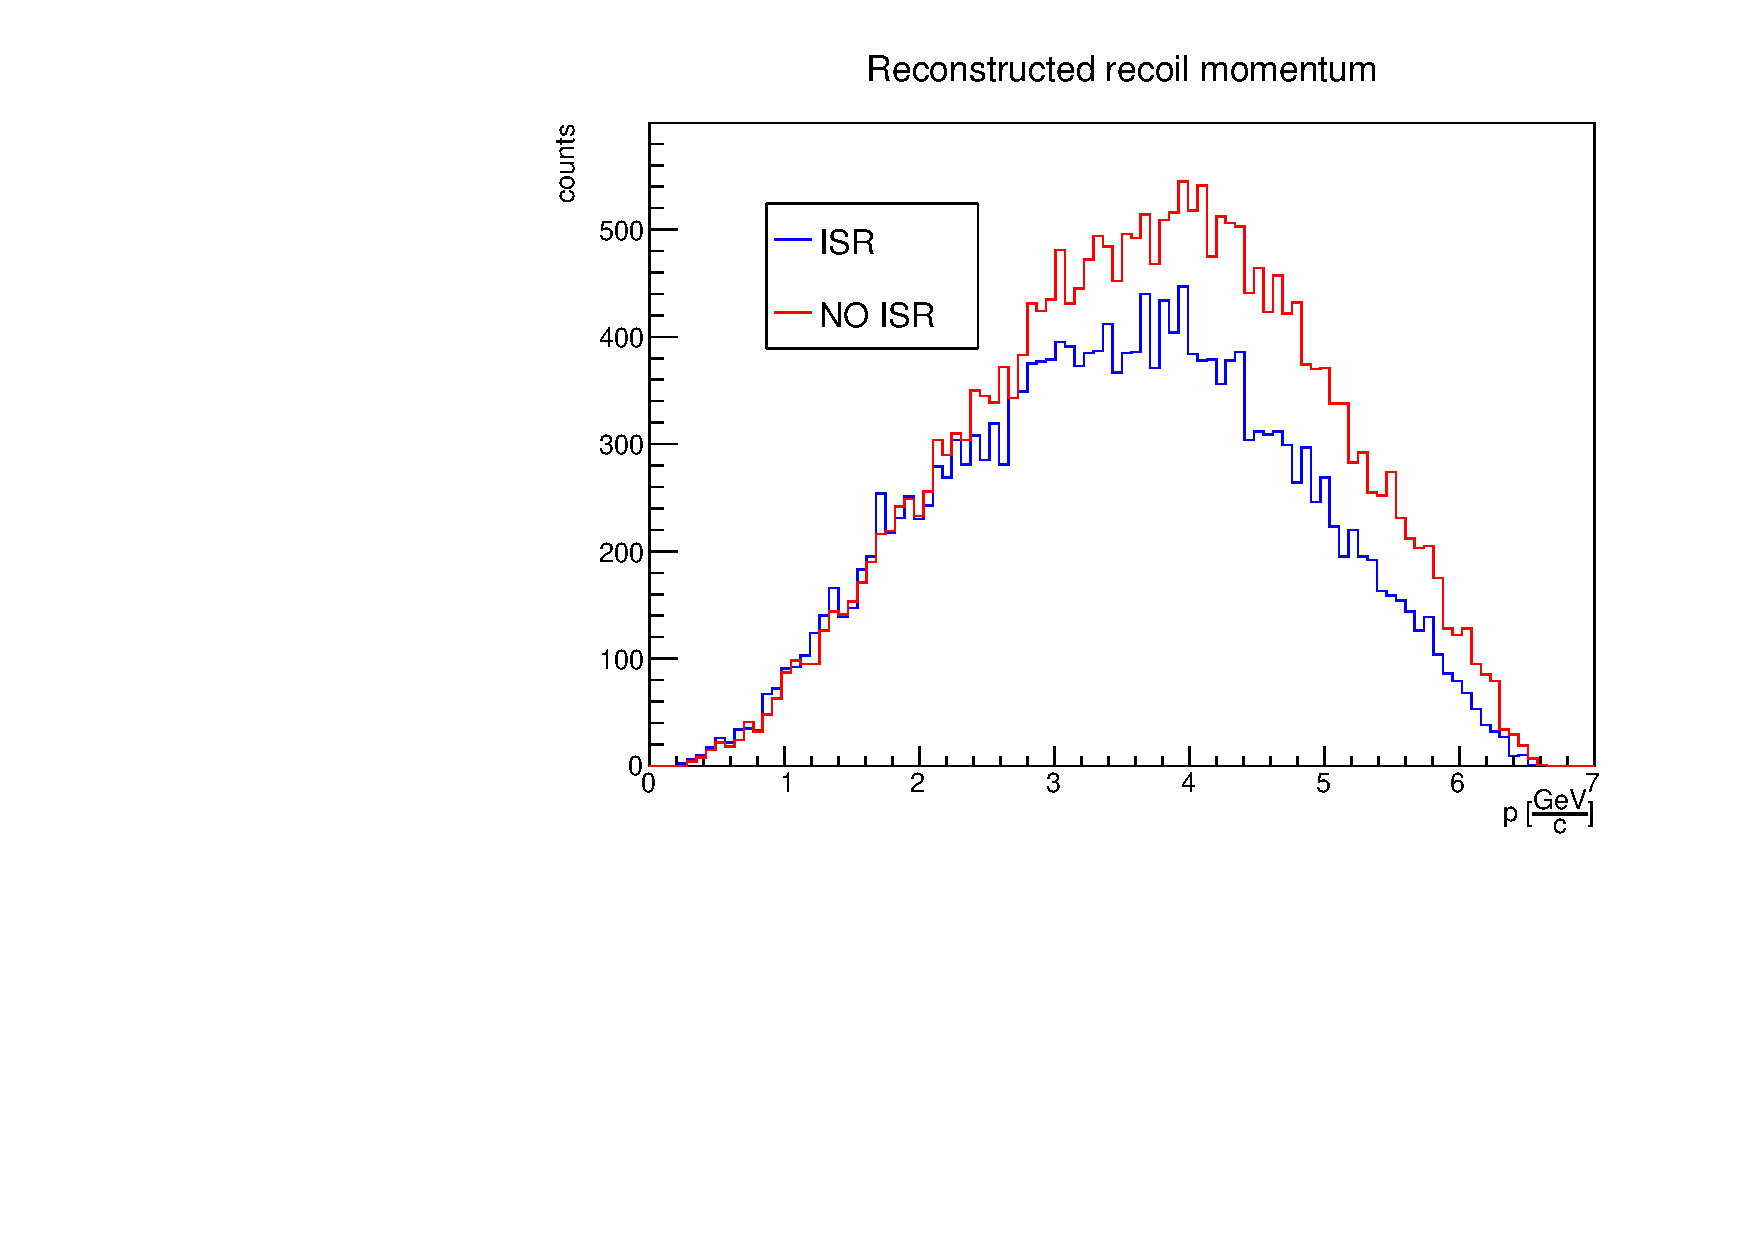
\includegraphics[width=0.70\textwidth]{nbar_MC/images/pRecoil.pdf}
    \caption{Reconstructed momentum distribution of the recoil system, in both ISR and NO ISR cases}
\end{figure}

Since the recoil system is well reconstructed through the recoil mass, it could be interesting to compare this distribution with that of $\bar{n}$, both from reconstruction and from generator. The latter is not affected by detector propagation and therefore it represents the $\bar{n}$ candidates generated momentum, free from misidentification and directly originating from the generator. The aforementioned $\bar{n}$ distributions are shown below:

\begin{figure}[H]
    \centering
    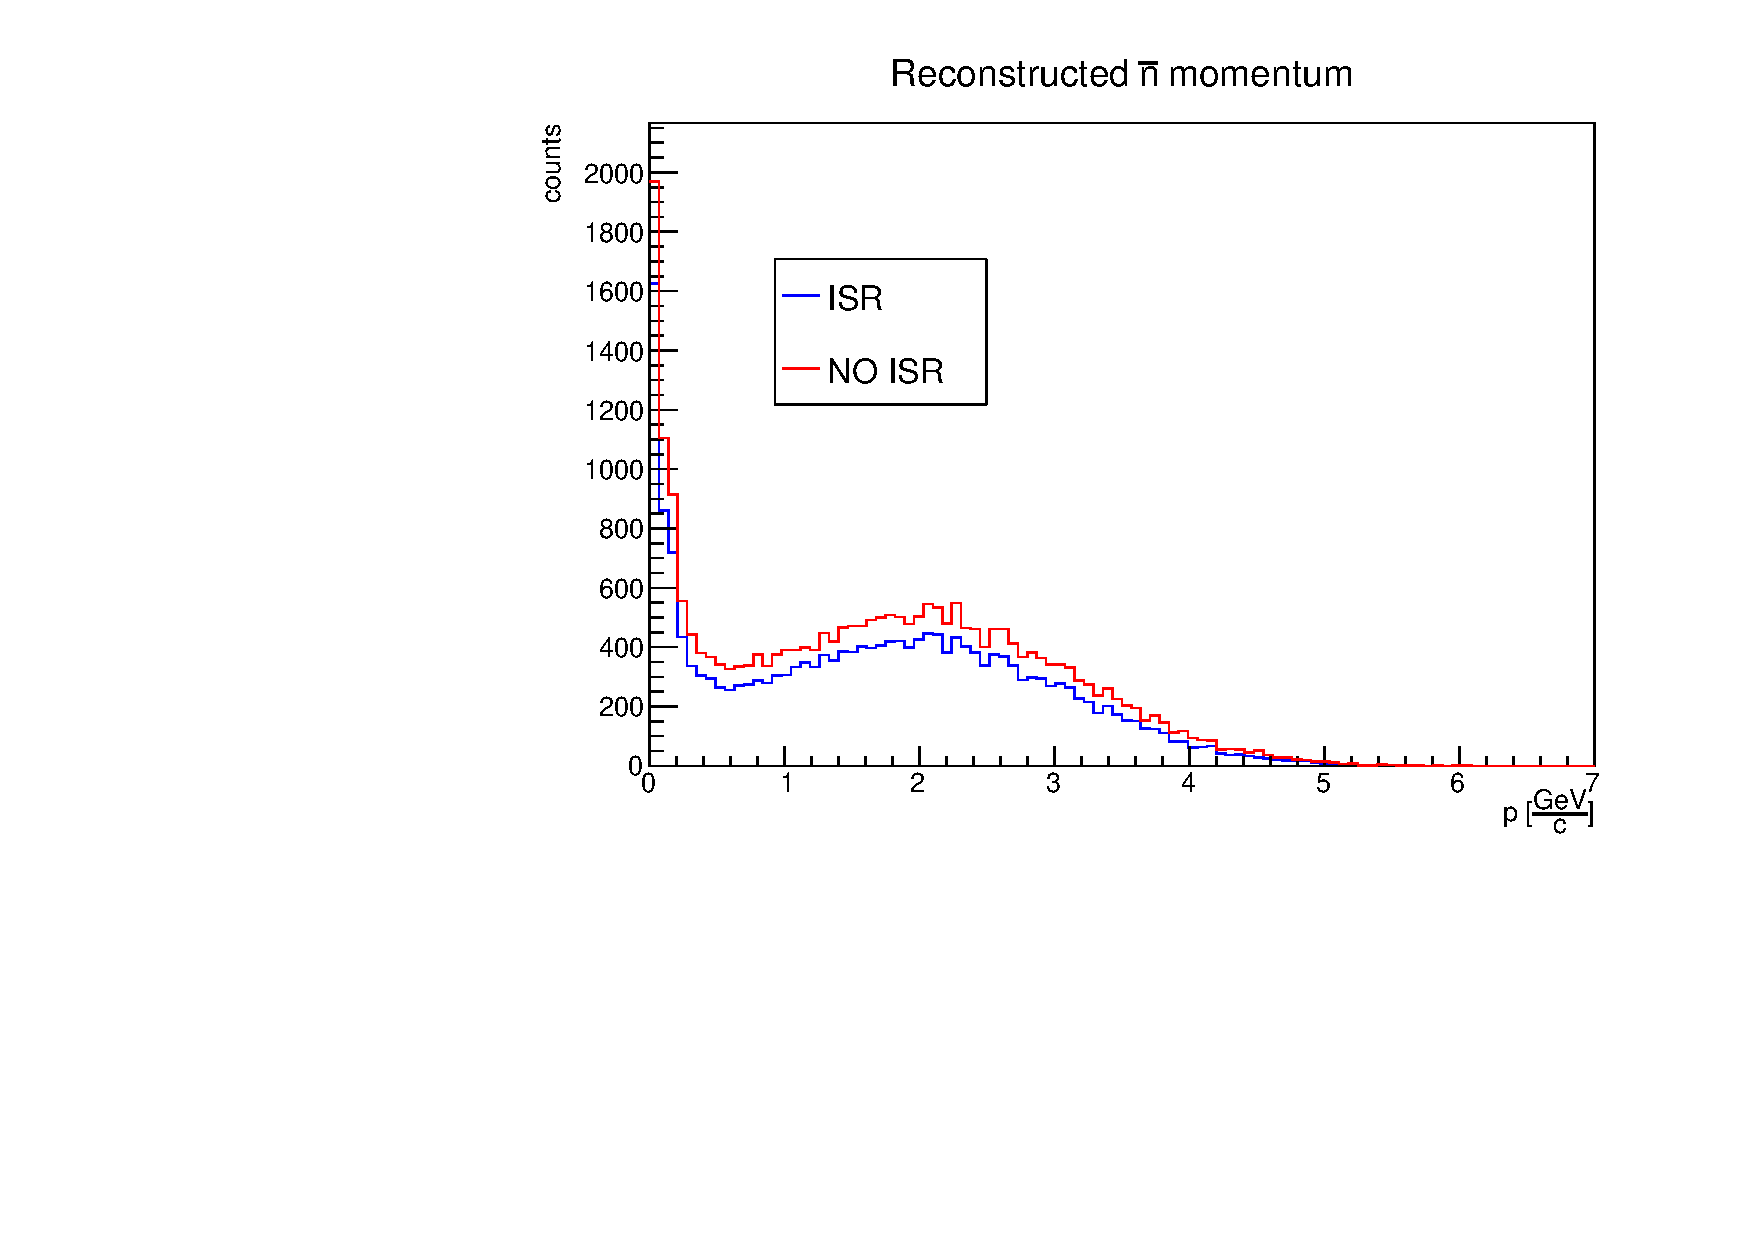
\includegraphics[width=0.49\textwidth]{nbar_MC/images/nbar_p.pdf}
    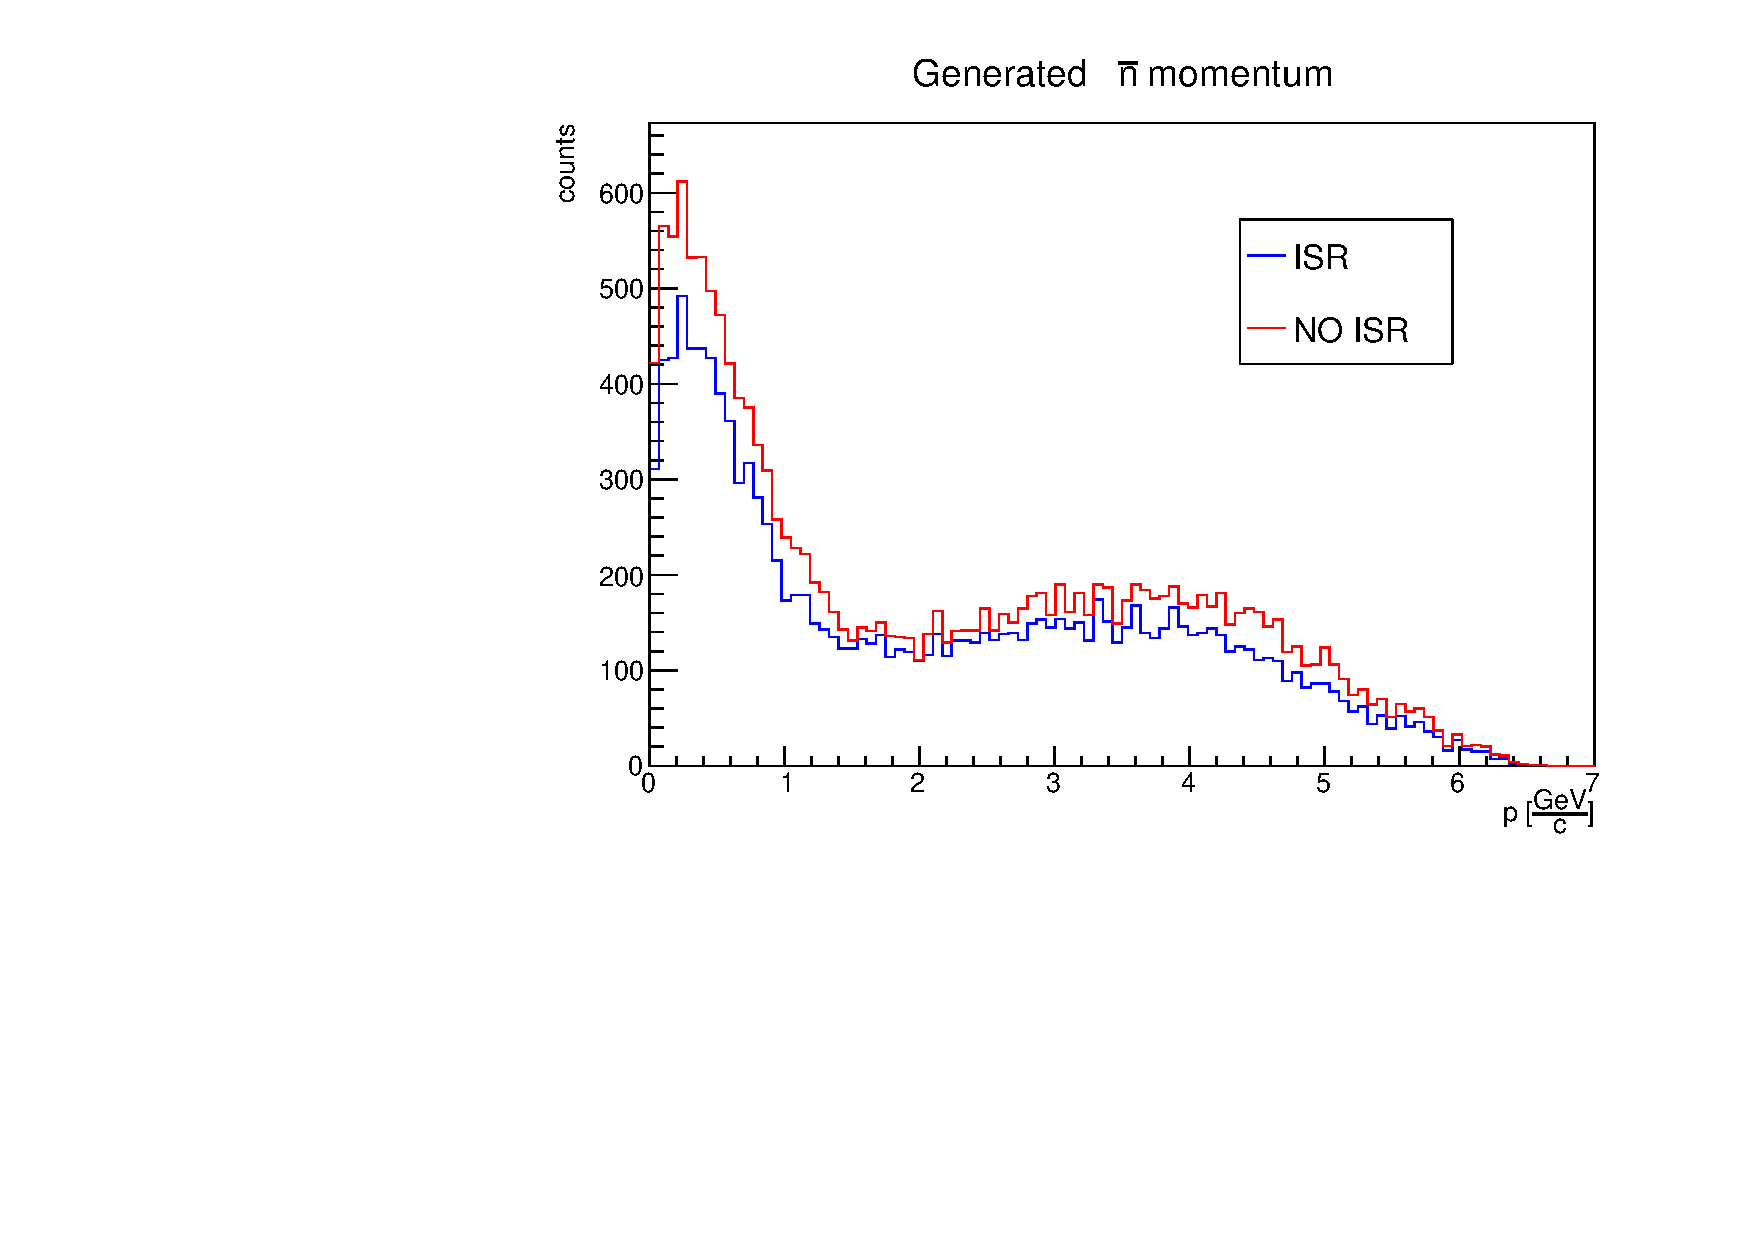
\includegraphics[width=0.49\textwidth]{nbar_MC/images/nbar_mcP.pdf}
    \caption{Reconstructed (left) and generated (right) momentum distribution of anti-neutron candidates, in both ISR and NO ISR cases}
\end{figure}

Notably, the reconstructed $\bar{n}$ momentum is systematically underestimated compared to the generator-level one, indicating missing energy within neutral clusters. This topic will be addressed in detail below through the momentum residuals.
$\\$
Both the reconstructed and generator-level distributions exhibit two structures, indicating two contributions within $\bar{n}$ candidate neutral clusters. To investigate this, the reconstructed recoil momentum is compared with the generator-level momentum of all $\bar{n}$ candidates, using MC truth matching. Since the $\bar{n}$ PDG code is \textbf{-2112}, the neutral clusters associated to $\bar{n}$ list can be matched to \textbf{true} (truth = 1) $\bar{n}$ particles, using Monte Carlo PDG $= -2112$, or to \textbf{false} (truth = 0) candidates with Monte Carlo PDG $\ne -2112$:

\begin{figure}[H]
    \centering
    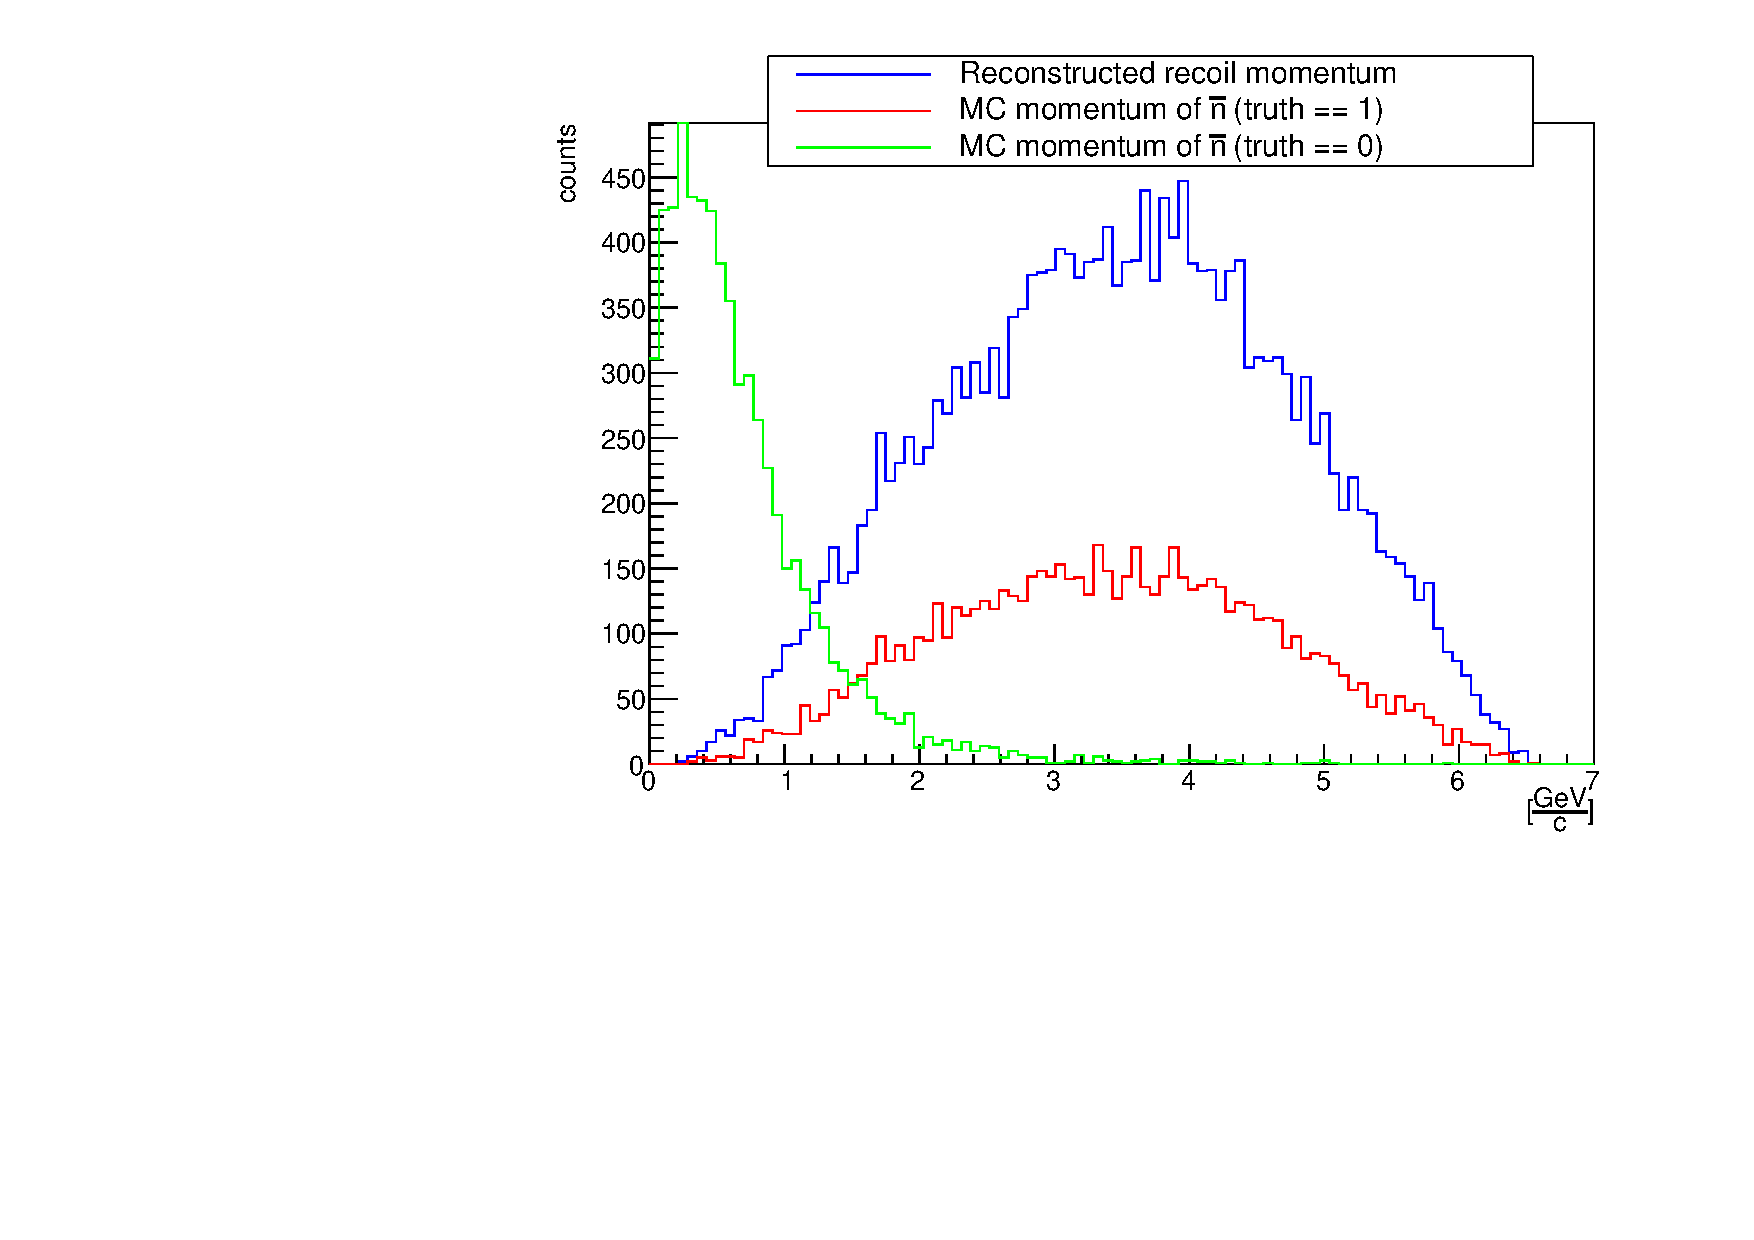
\includegraphics[width=0.49\textwidth]{nbar_MC/images/pRecoil_nmcP_isr.pdf}
    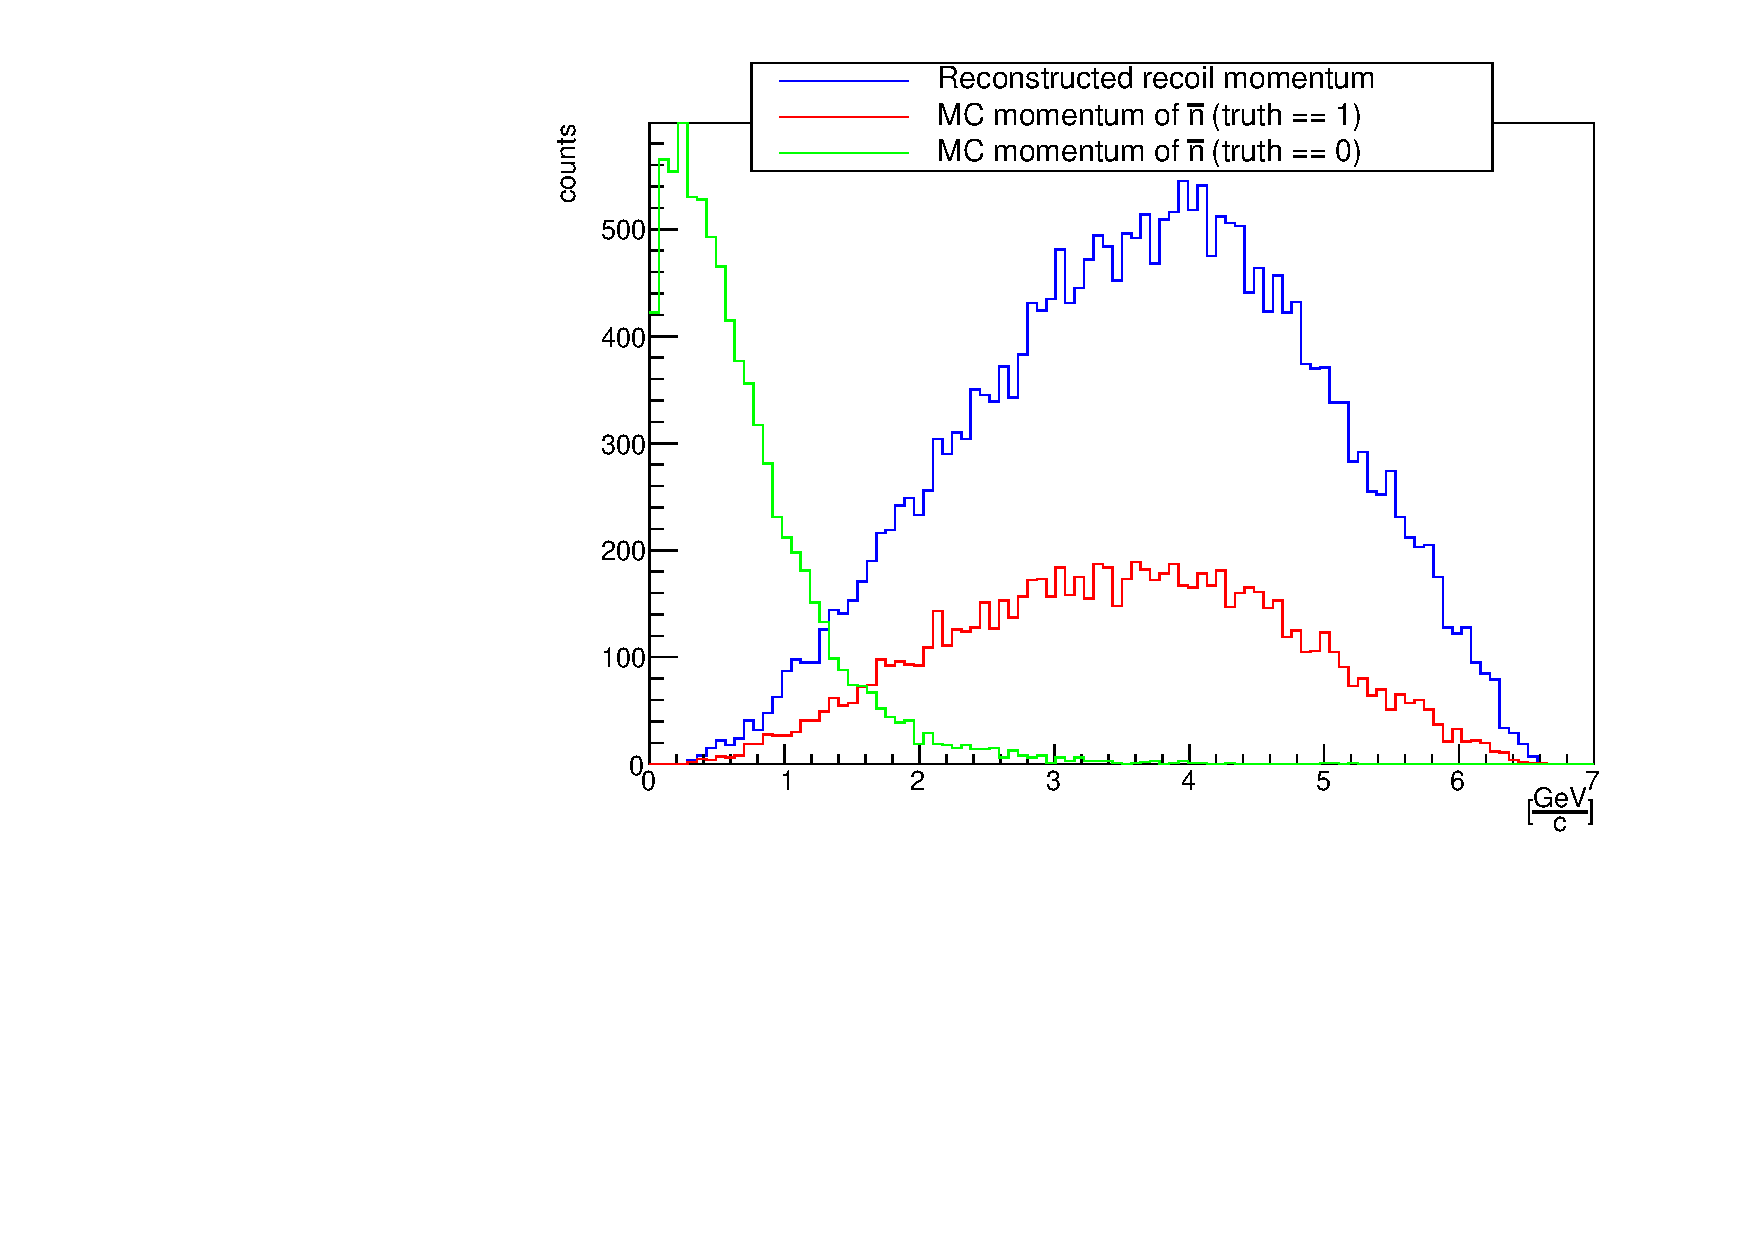
\includegraphics[width=0.49\textwidth]{nbar_MC/images/pRecoil_nmcP_nog.pdf}
    \caption{(left) Momentum contribution component in ISR case \\ (right) Momentum contribution component in NO ISR case}  
    \label{fig:pRecoil_nmcP} 
\end{figure}
    
As expected, the low-momentum structure corresponds to candidates not associated to $\bar{n}$ by the Monte Carlo truth, exhibiting significant deviation from the recoil momentum. This is likely due to cluster split-off and/or pre-showering effects as will be discussed later. Furthermore, the {\color{red} red distribution} is include within the {\color{blue} blue one}, suggesting that several anti-neutron are missing after the reconstruction. All these aspects will be discussed in the next section through analysis of $\bar{n}$ relatives (ancestors).      
$\\$
To compare the reconstructed recoil with the Monte Carlo matched $\bar{n}$ (truth = 1), it is useful to analyze their linear correlation coefficient $\rho$, recalling that:
\begin{center}
$\rho_{x,y} = \frac{cov[x,y]}{\sigma_x \sigma_y} $ \hspace{0.5cm} where $cov[x,y] = E[xy] - E[x]E[y]$
\end{center}

Therefore, the correlations in $\theta$, for both the reconstructed and the generated case, are shown below:

\begin{figure}[H]
    \centering
     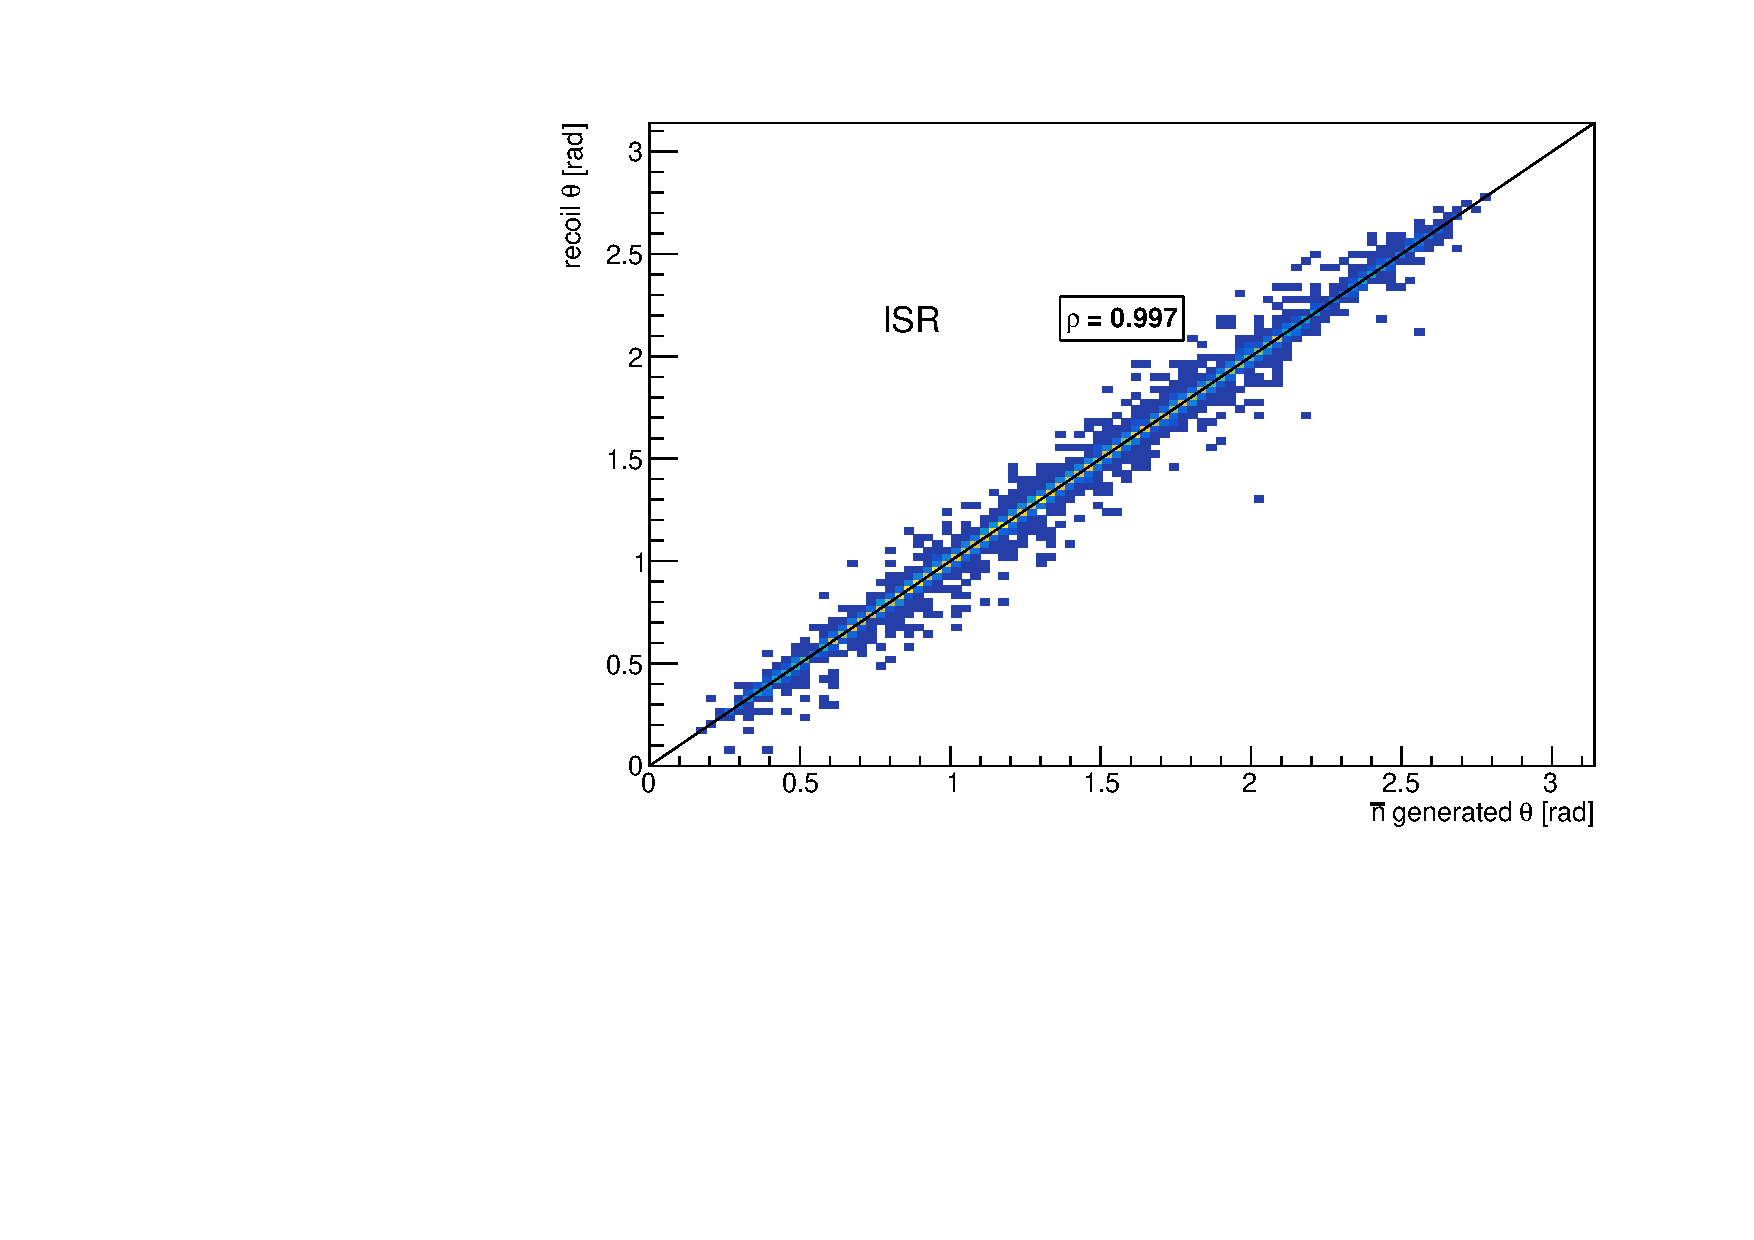
\includegraphics[width=0.49\textwidth]{nbar_MC/images/gen_mc_theta_corr_isr.pdf}
     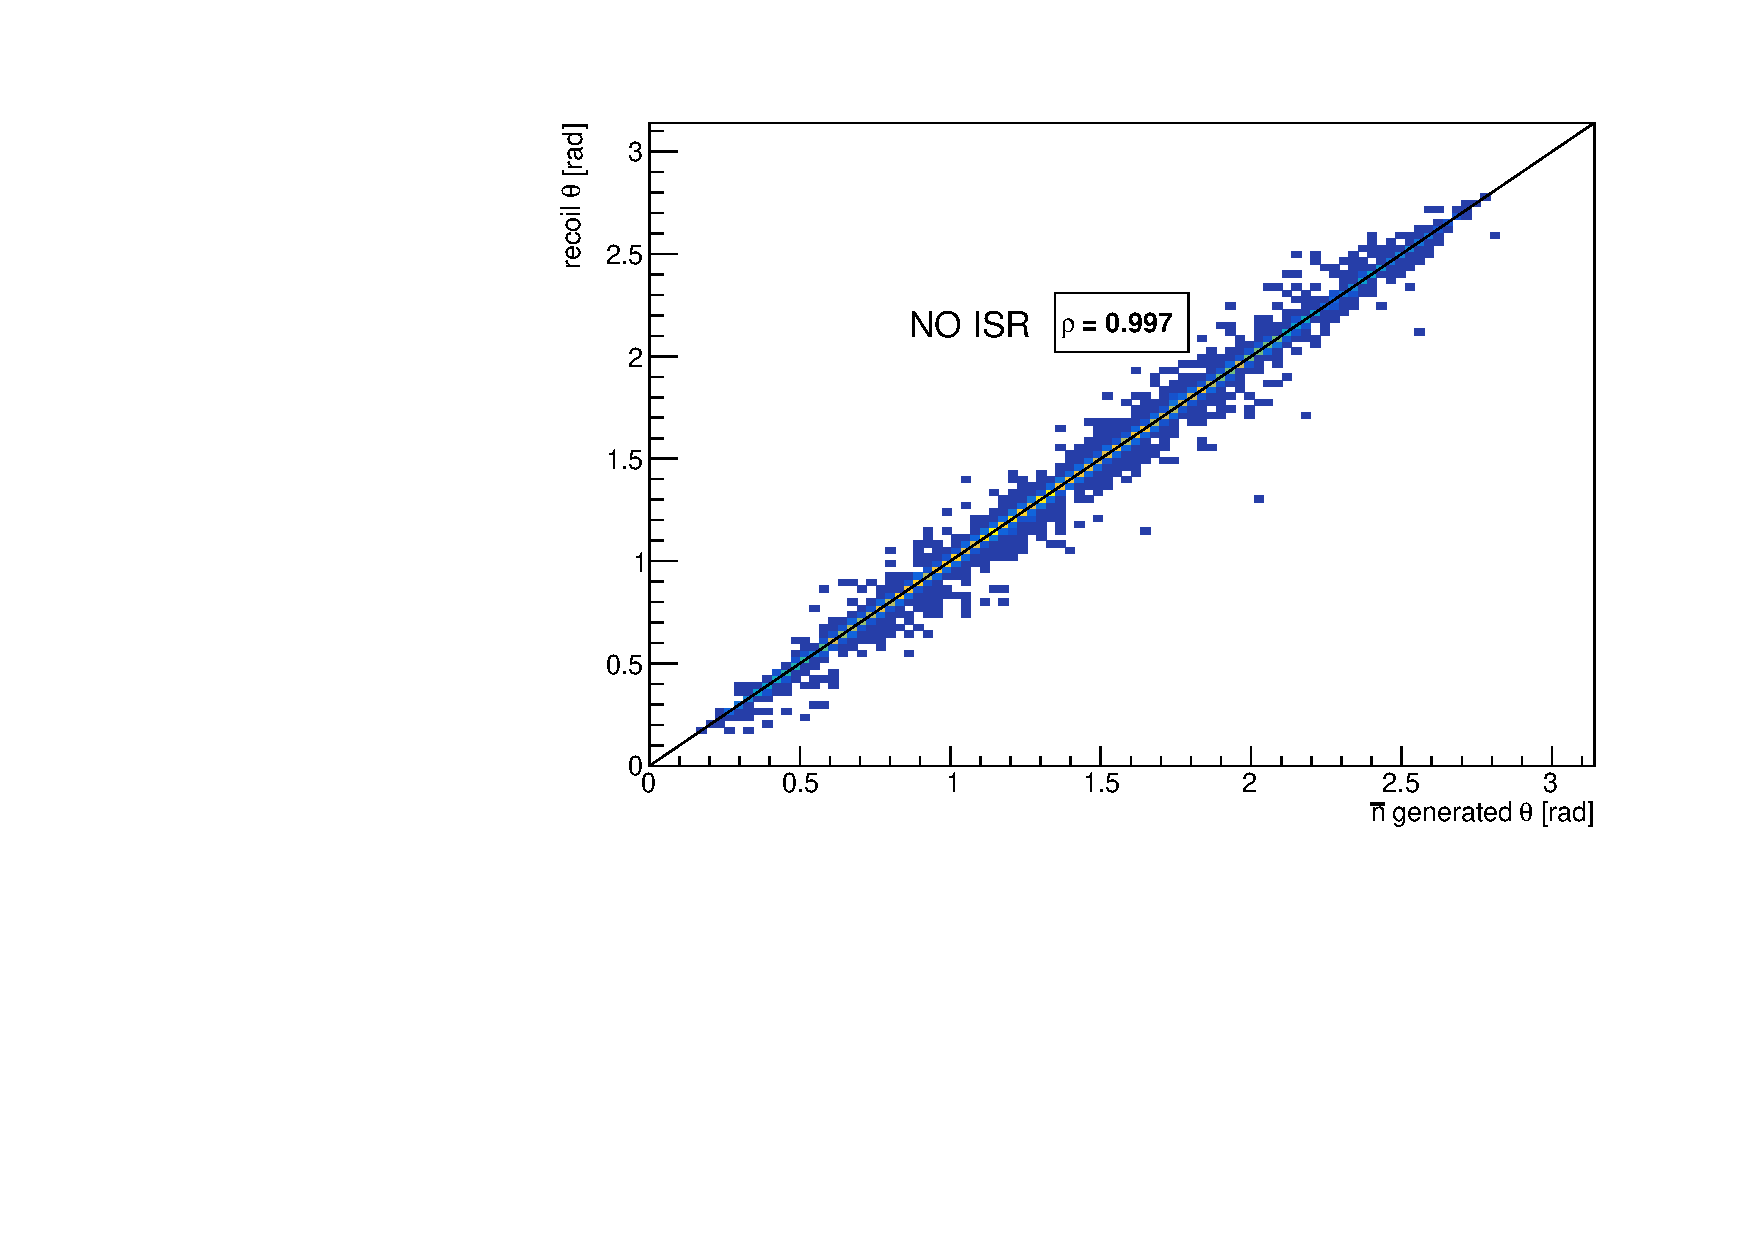
\includegraphics[width=0.49\textwidth]{nbar_MC/images/gen_mc_theta_corr_nog.pdf}
     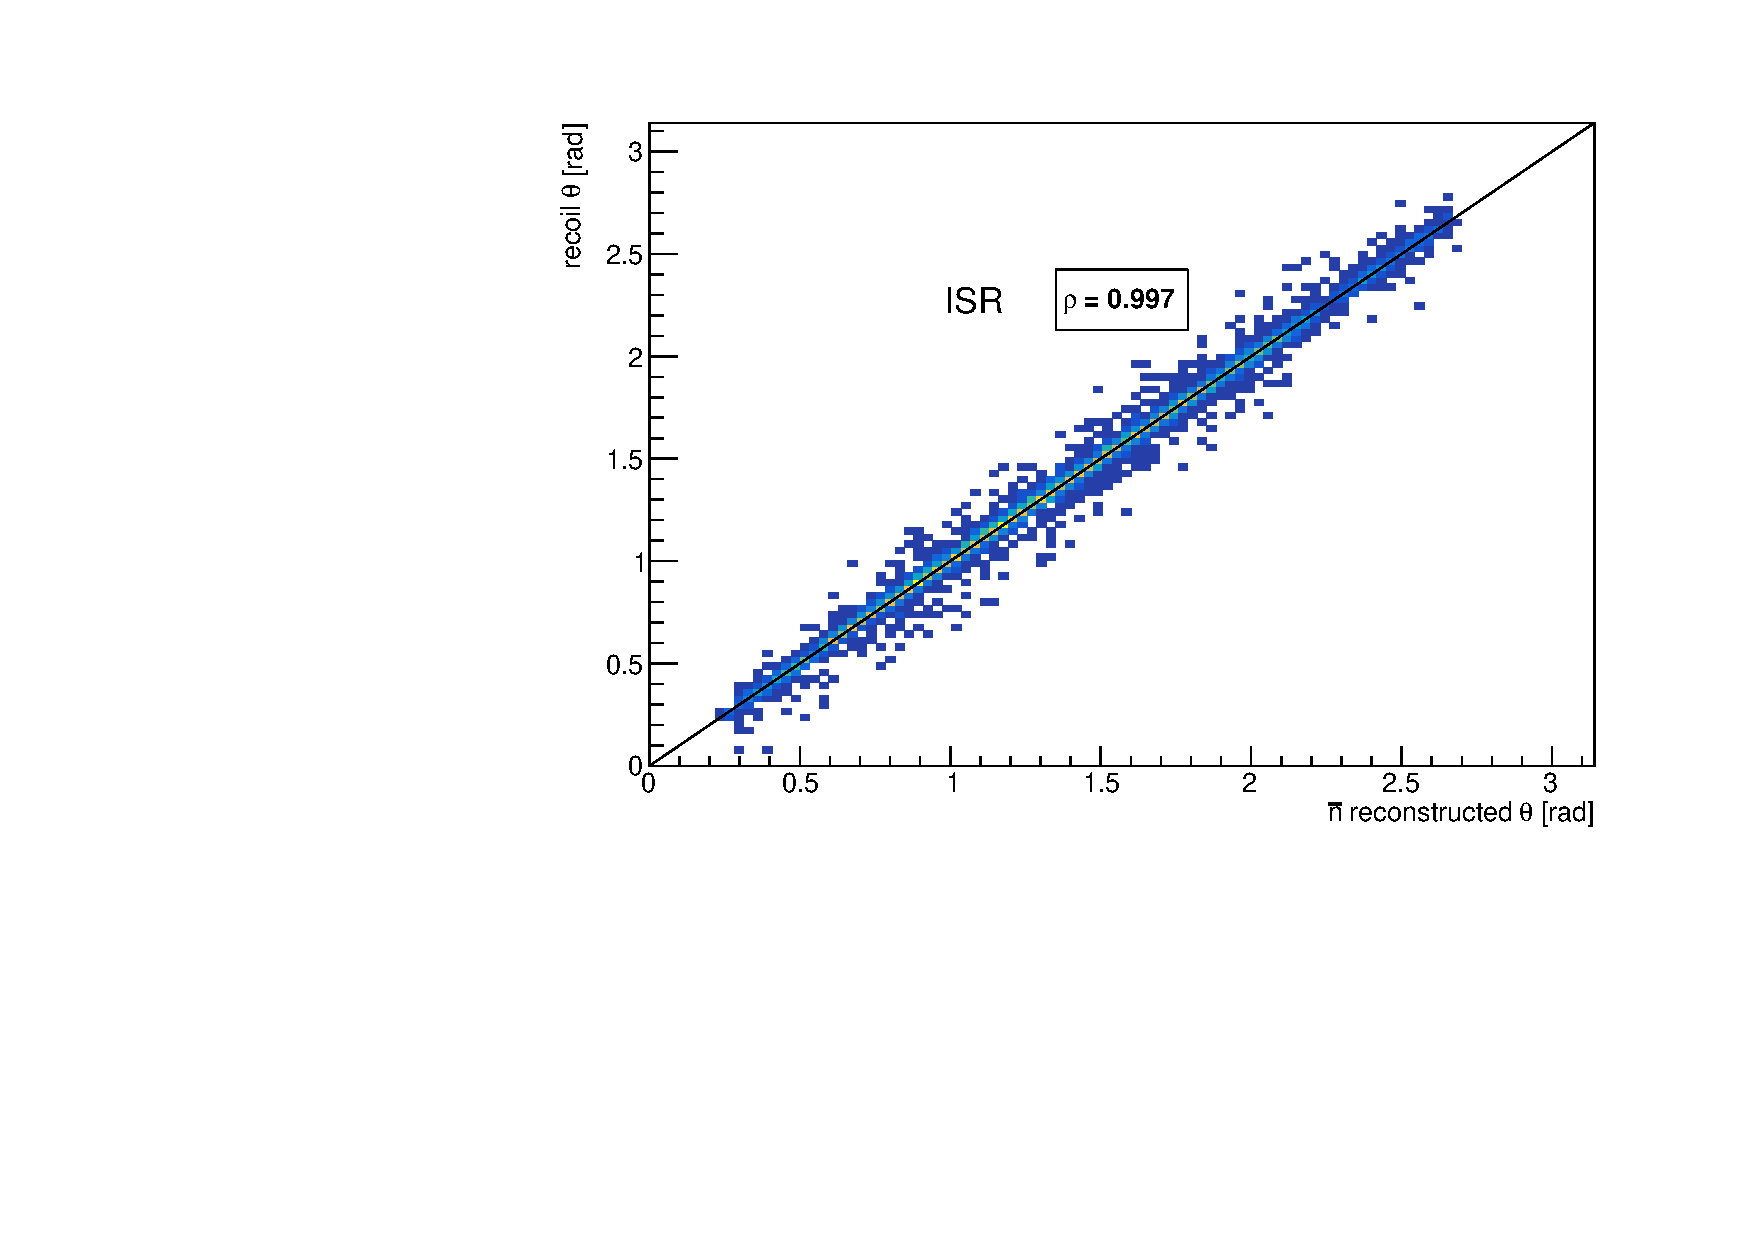
\includegraphics[width=0.49\textwidth]{nbar_MC/images/gen_rec_theta_corr_isr.pdf}
     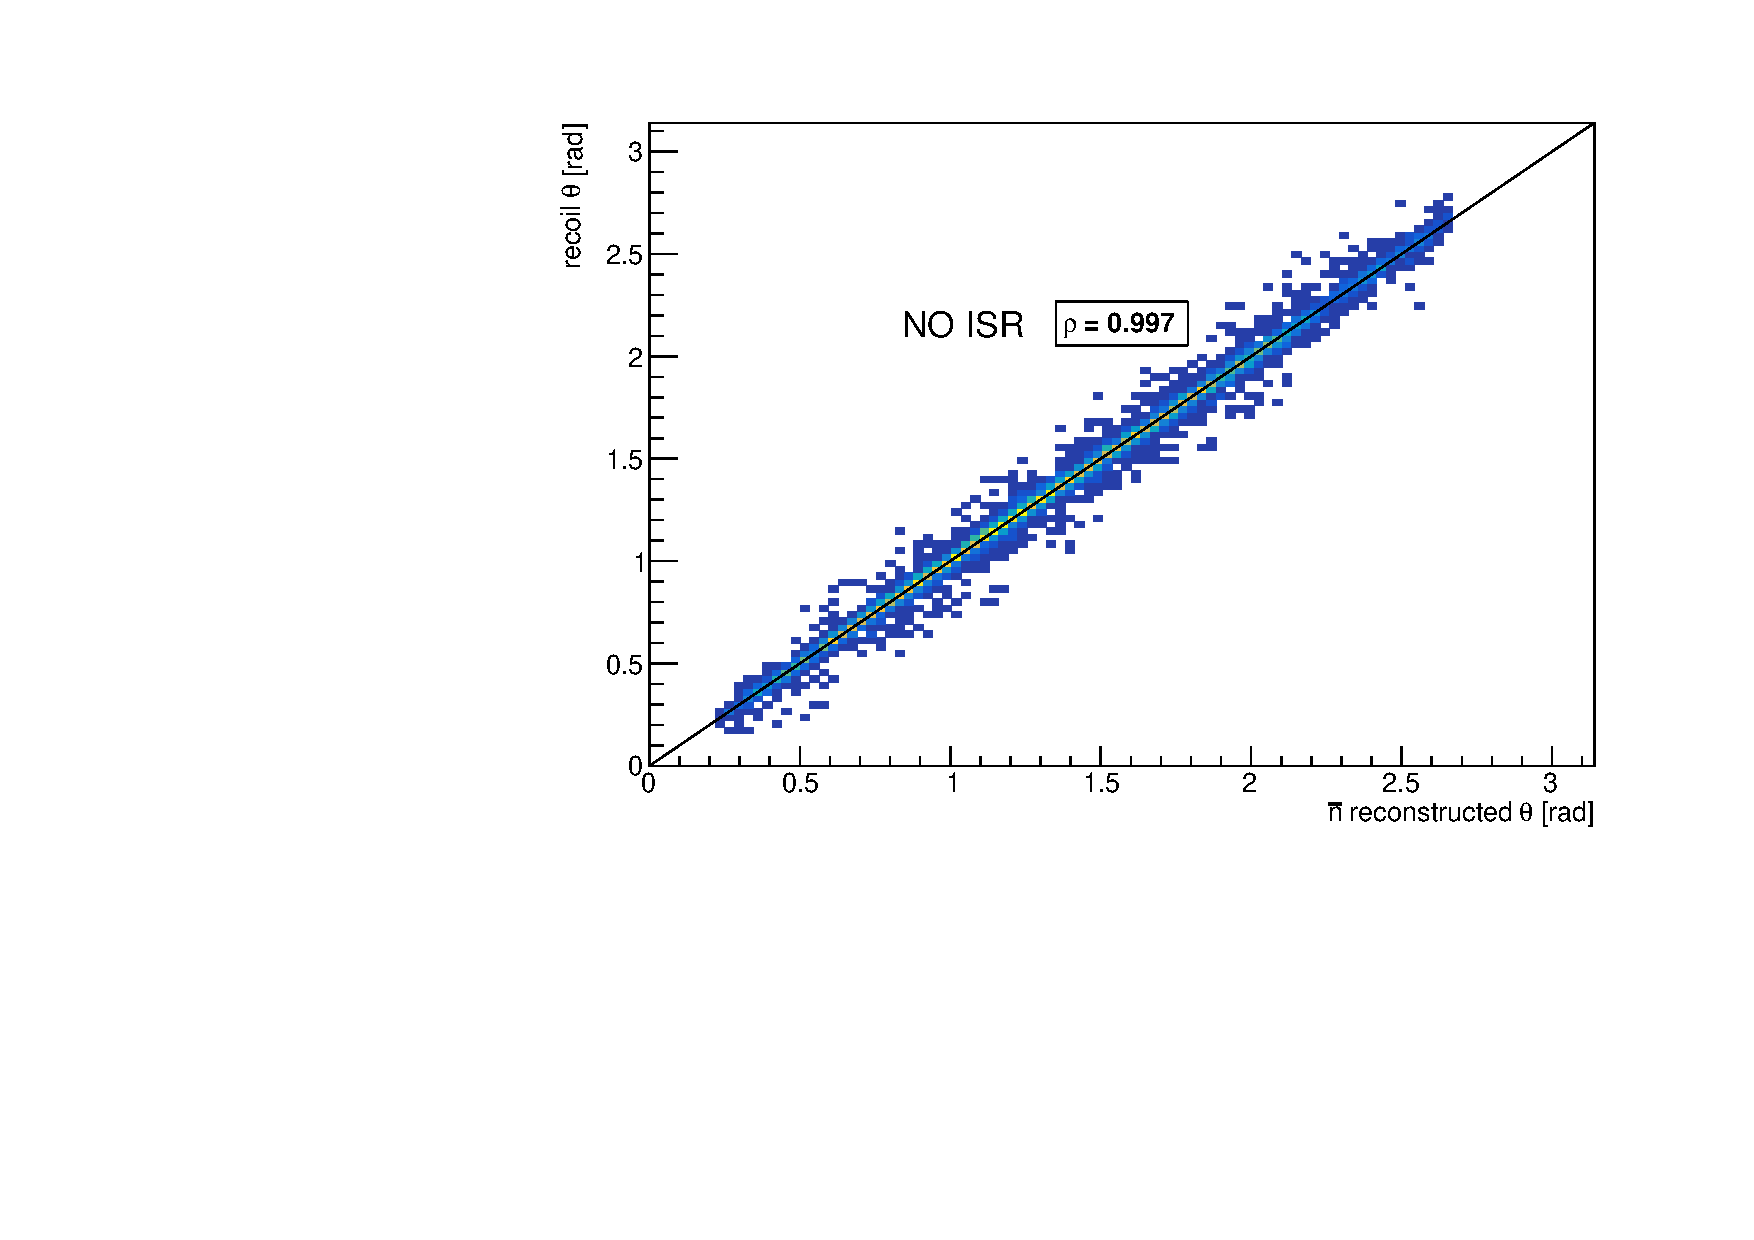
\includegraphics[width=0.49\textwidth]{nbar_MC/images/gen_rec_theta_corr_nog.pdf}
      \caption{$\theta$ correlation distribution between recoil system and anti-neutron candidate, in both reconstructed and generated case. Linear correlation coefficient $\rho$ truncated to three decimal places}
\end{figure}

A good correlation can be highlighted between the two distributions in both reconstructed and generator-level cases, indicating that the the anti-neutron $\theta$ direction is properly described.
$\\$
The same comparison can be addressed for the momentum, remembering that it is obtained starting from the energy of the cluster as follow:
 \begin{center}
$p_{rec}^2 = E_{ECL}^2 - m_{\bar{n}}^2$
\end{center}

The obtained conjugate distributions are shown below:
\begin{figure}[H]
    \centering
     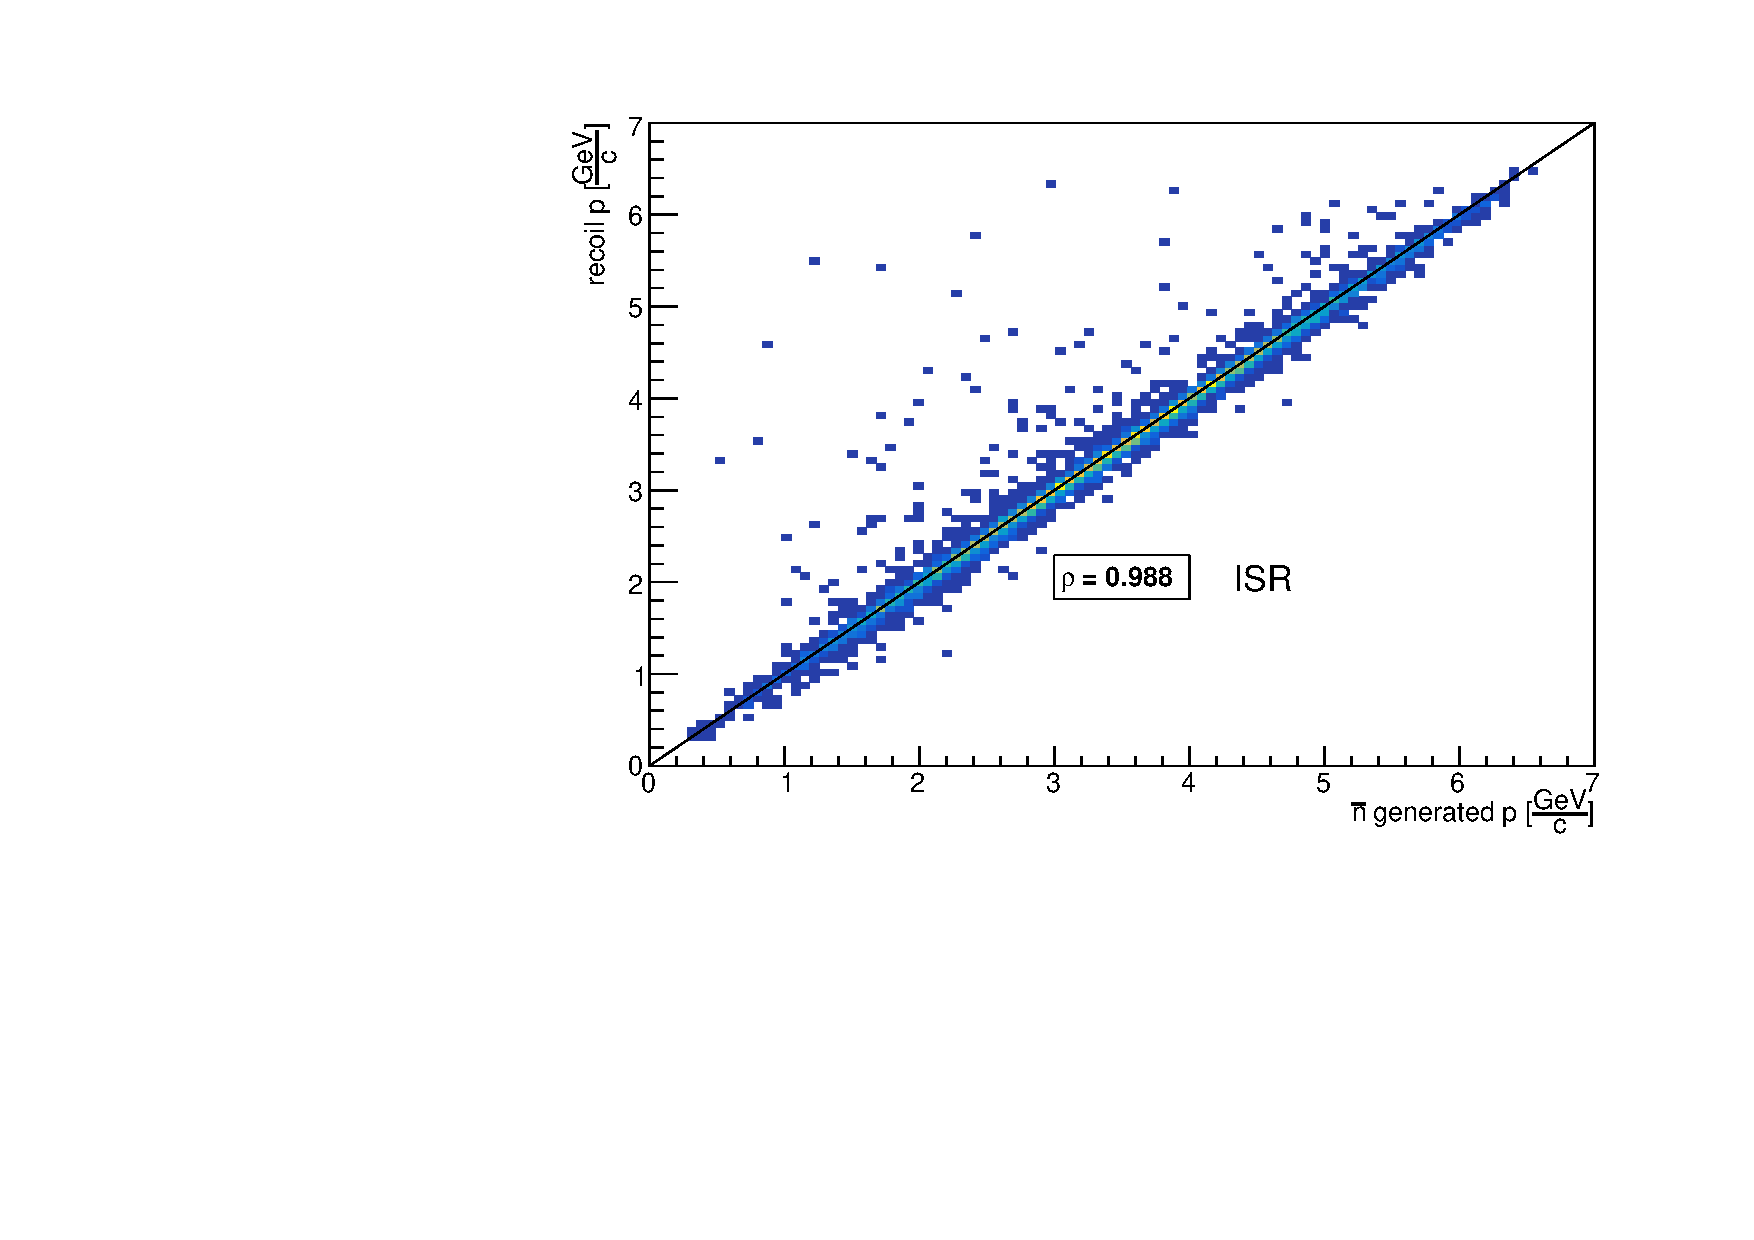
\includegraphics[width=0.49\textwidth]{nbar_MC/images/gen_mc_p_corr_isr.pdf}
     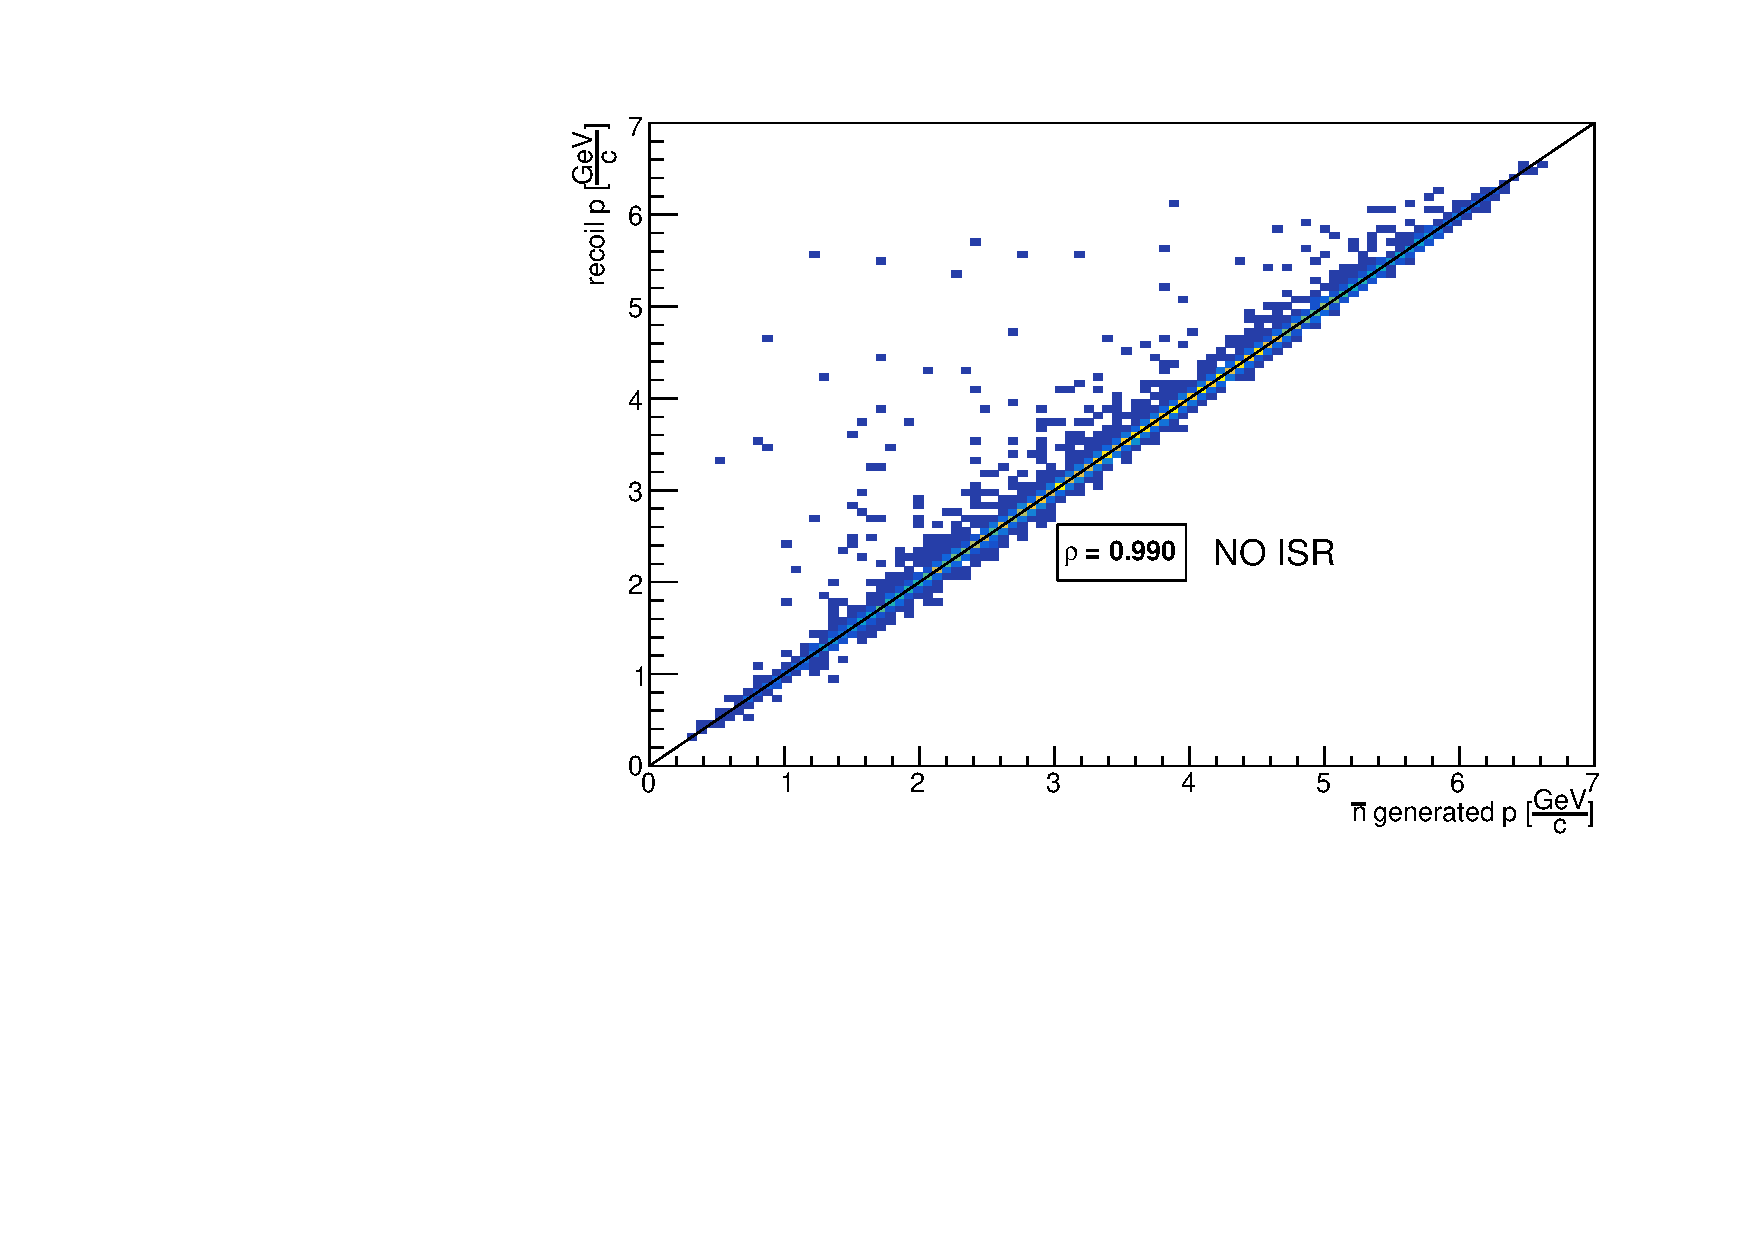
\includegraphics[width=0.49\textwidth]{nbar_MC/images/gen_mc_p_corr_nog.pdf}
     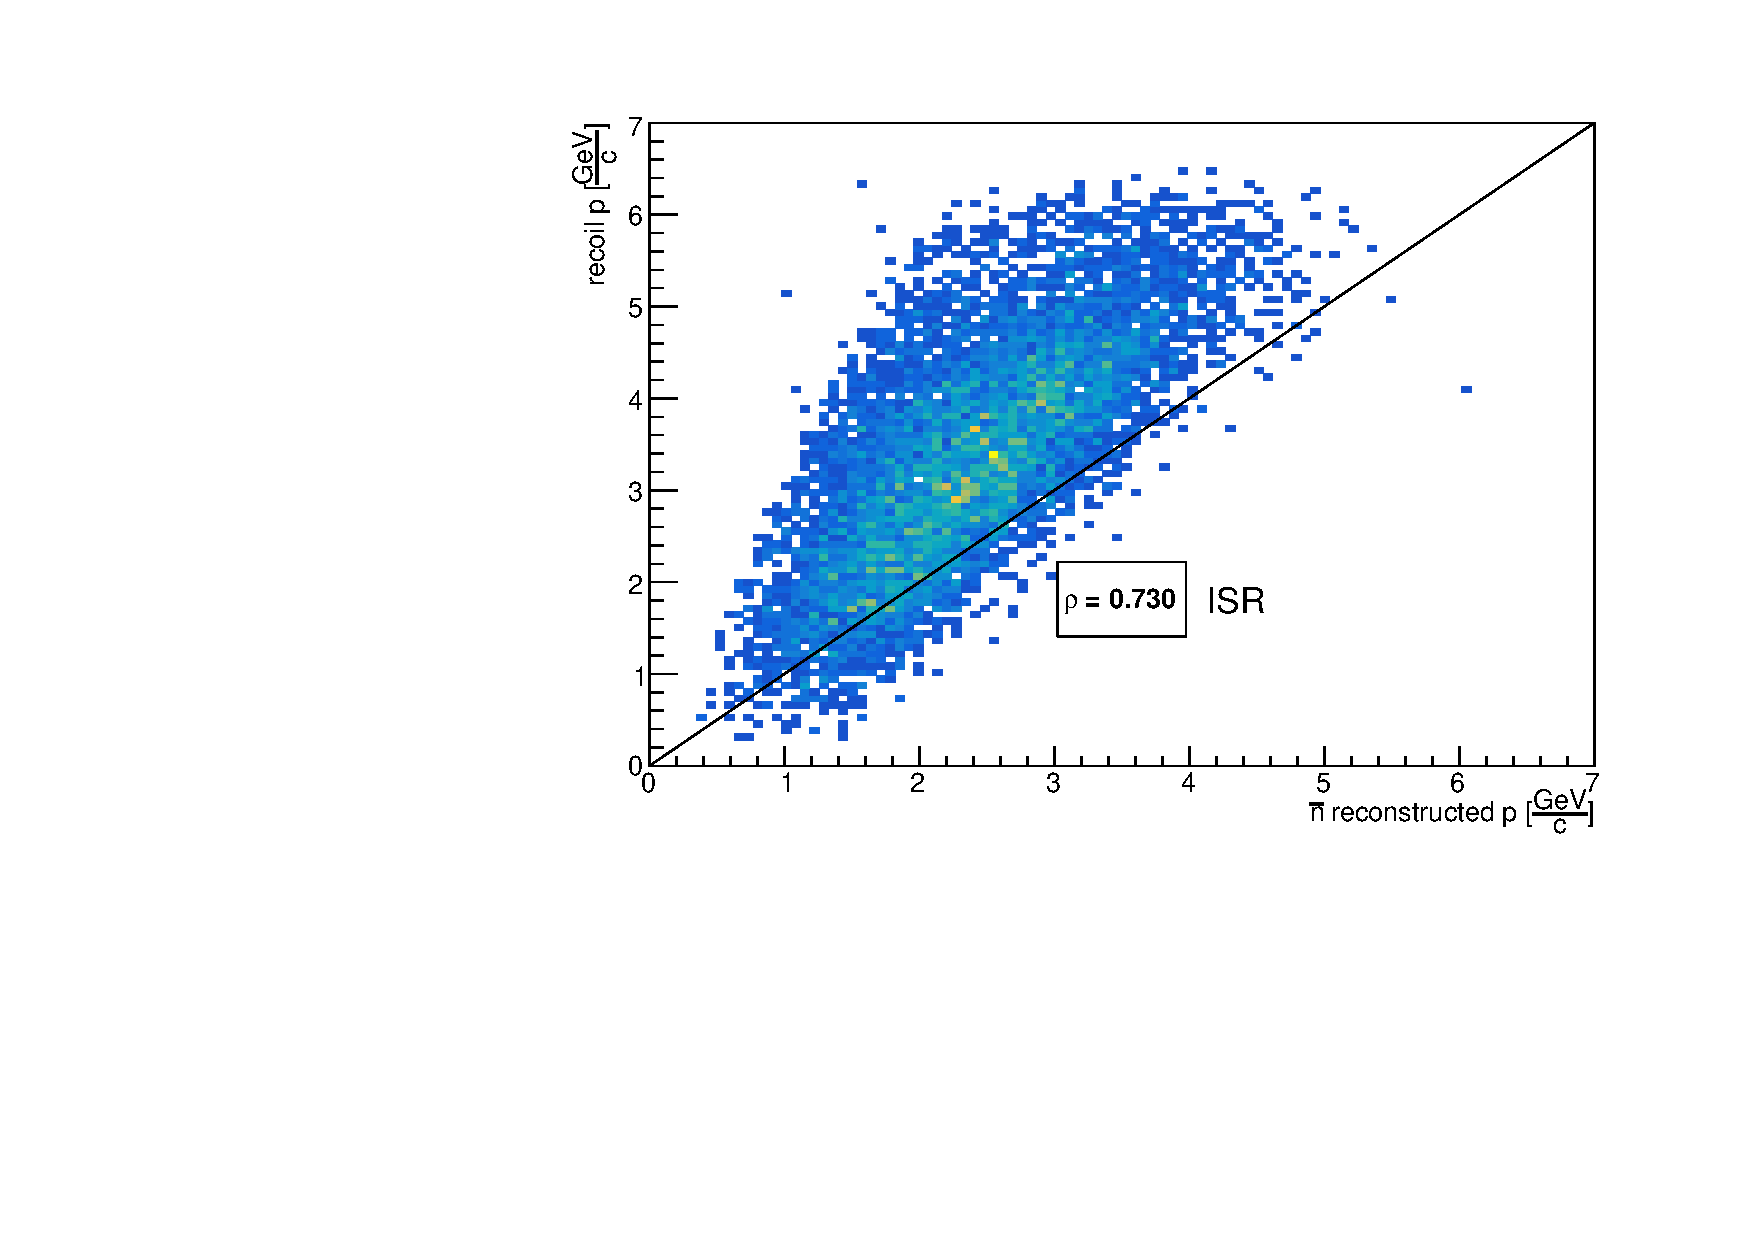
\includegraphics[width=0.49\textwidth]{nbar_MC/images/gen_rec_p_corr_isr.pdf}
     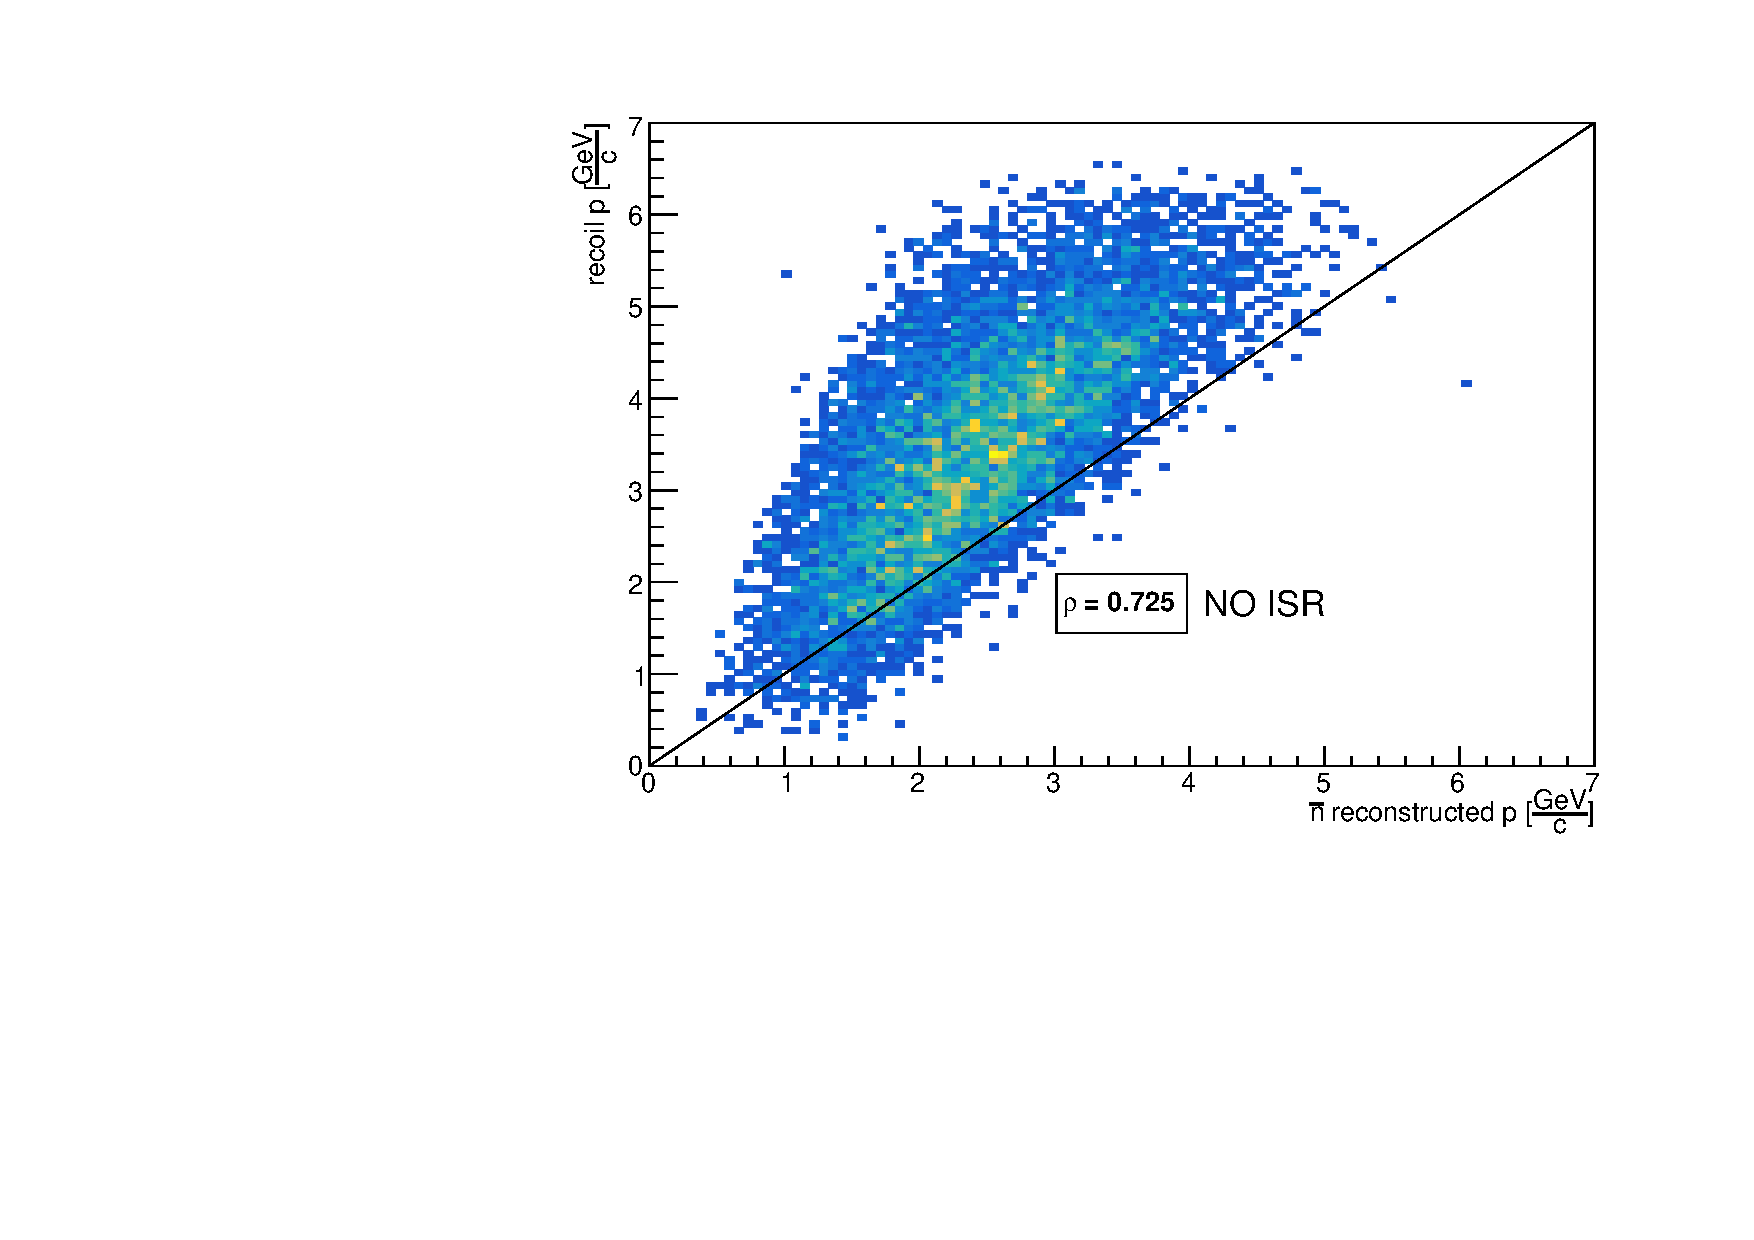
\includegraphics[width=0.49\textwidth]{nbar_MC/images/gen_rec_p_corr_nog.pdf}
      \caption{Momentum correlation distribution between recoil system and anti-neutron candidate, in both reconstructed and generated case. Linear correlation coefficient $\rho$ truncated to three decimal places}
      \label{fig:pRecoil-nP}
\end{figure}

A good correlation can be observed between the reconstructed recoil momentum and the generated $\bar{n}$ one, confirming how the first is properly describing the $\bar{n}$ kinematic.
$\\$
However, a poor resolution is observed in reconstructed $\bar{n}$ momentum, in both ISR and NO ISR cases, presenting an underestimation of the reconstructed $\bar{n}$ momentum as well. In order to directly study it, the momentum residual can be analyzed:
\begin{figure}[H]
    \centering
     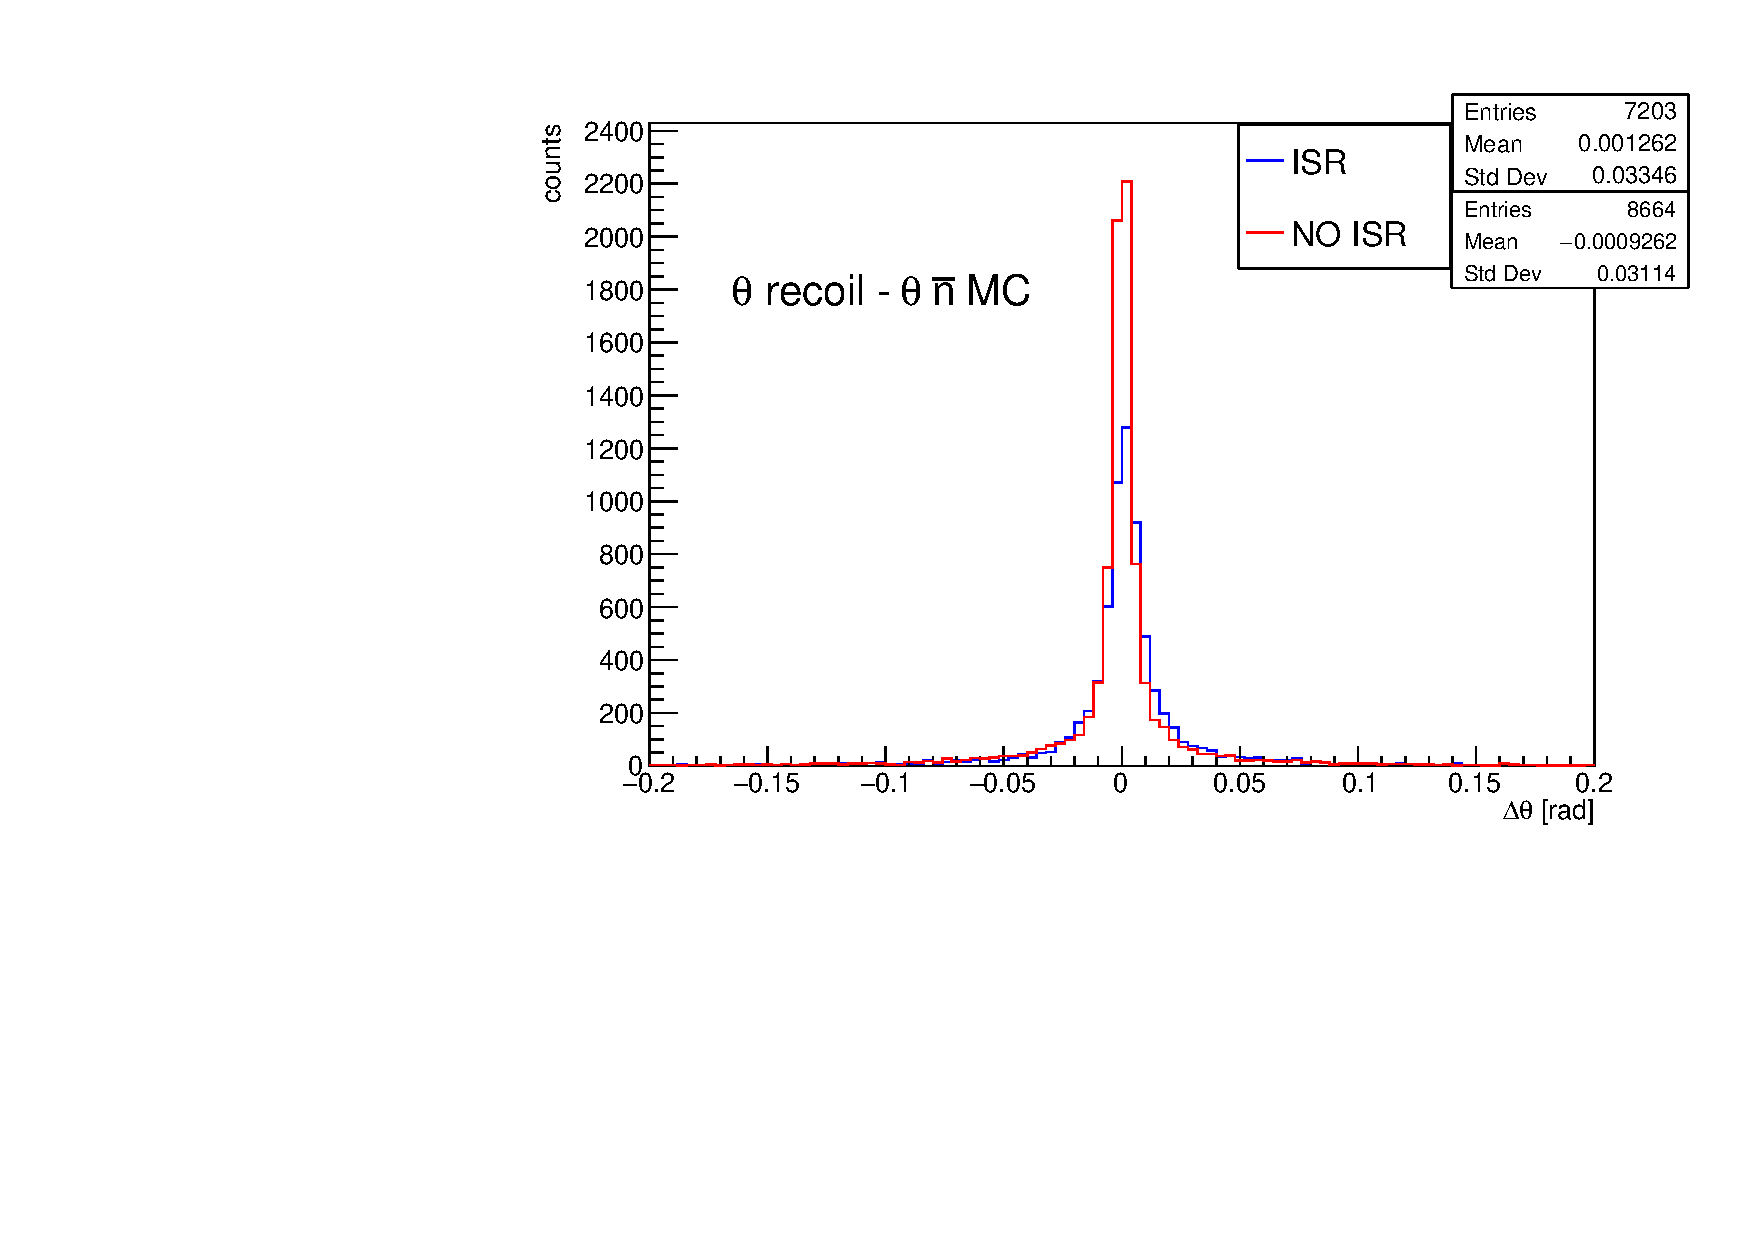
\includegraphics[width=0.49\textwidth]{nbar_MC/images/diff_thetaREC_ntheta_mc.pdf}
     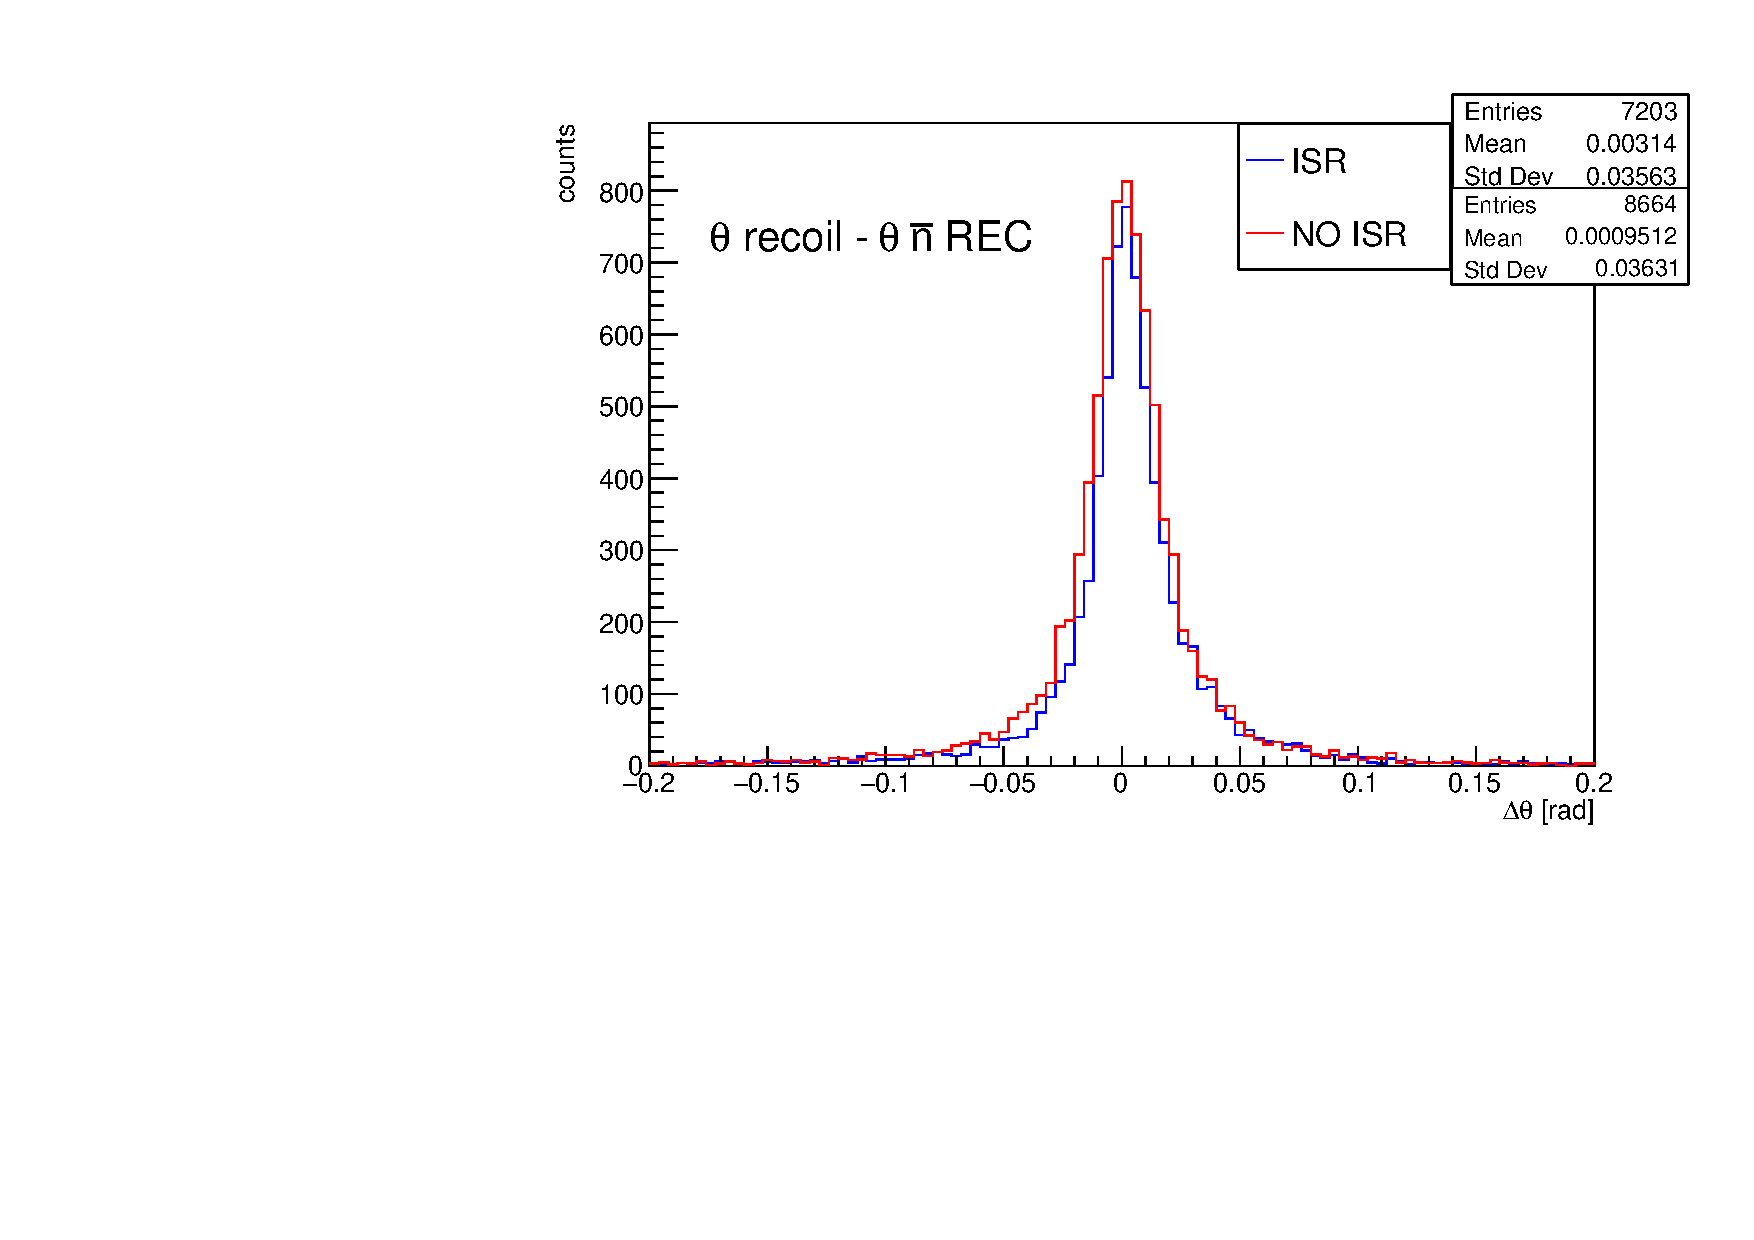
\includegraphics[width=0.49\textwidth]{nbar_MC/images/diff_thetaREC_ntheta_rec.pdf}
     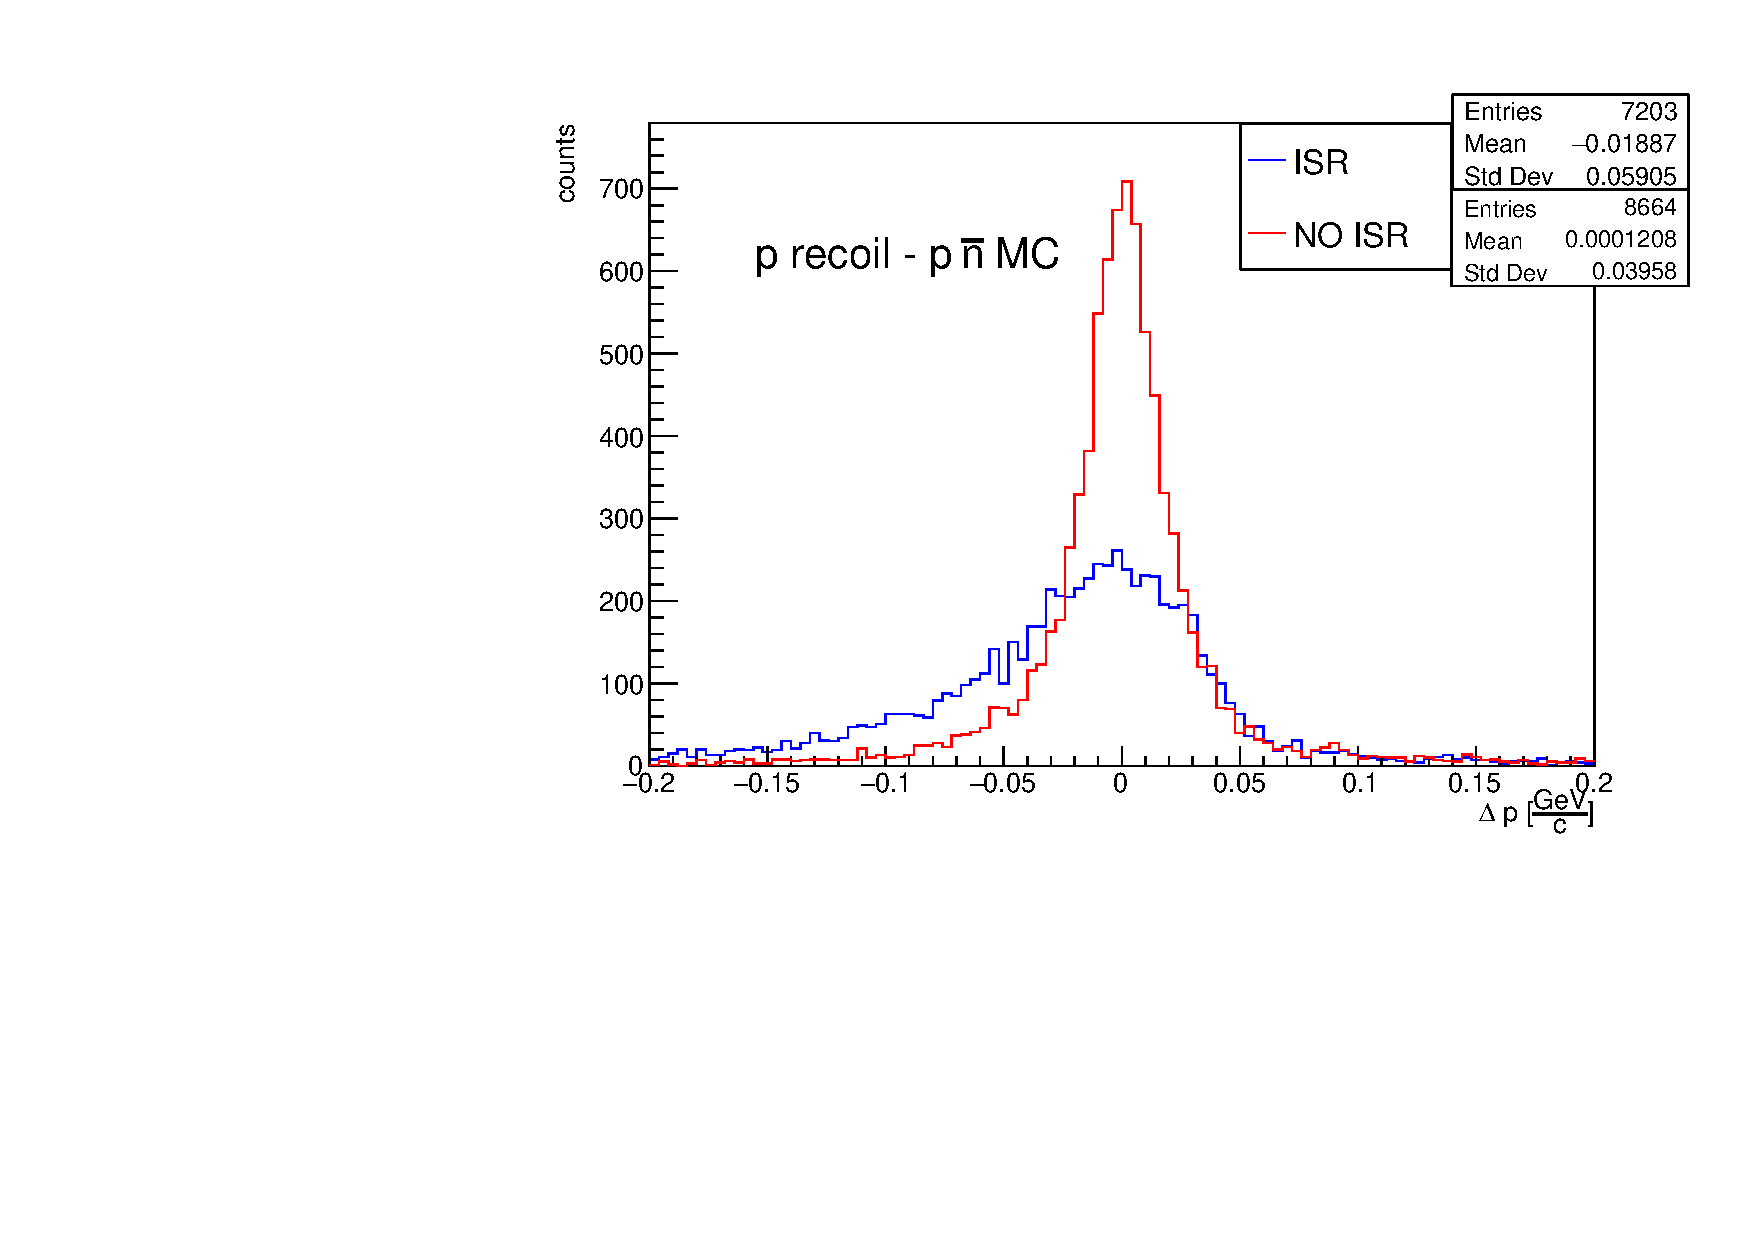
\includegraphics[width=0.49\textwidth]{nbar_MC/images/diff_pREC_np_mc.pdf}
     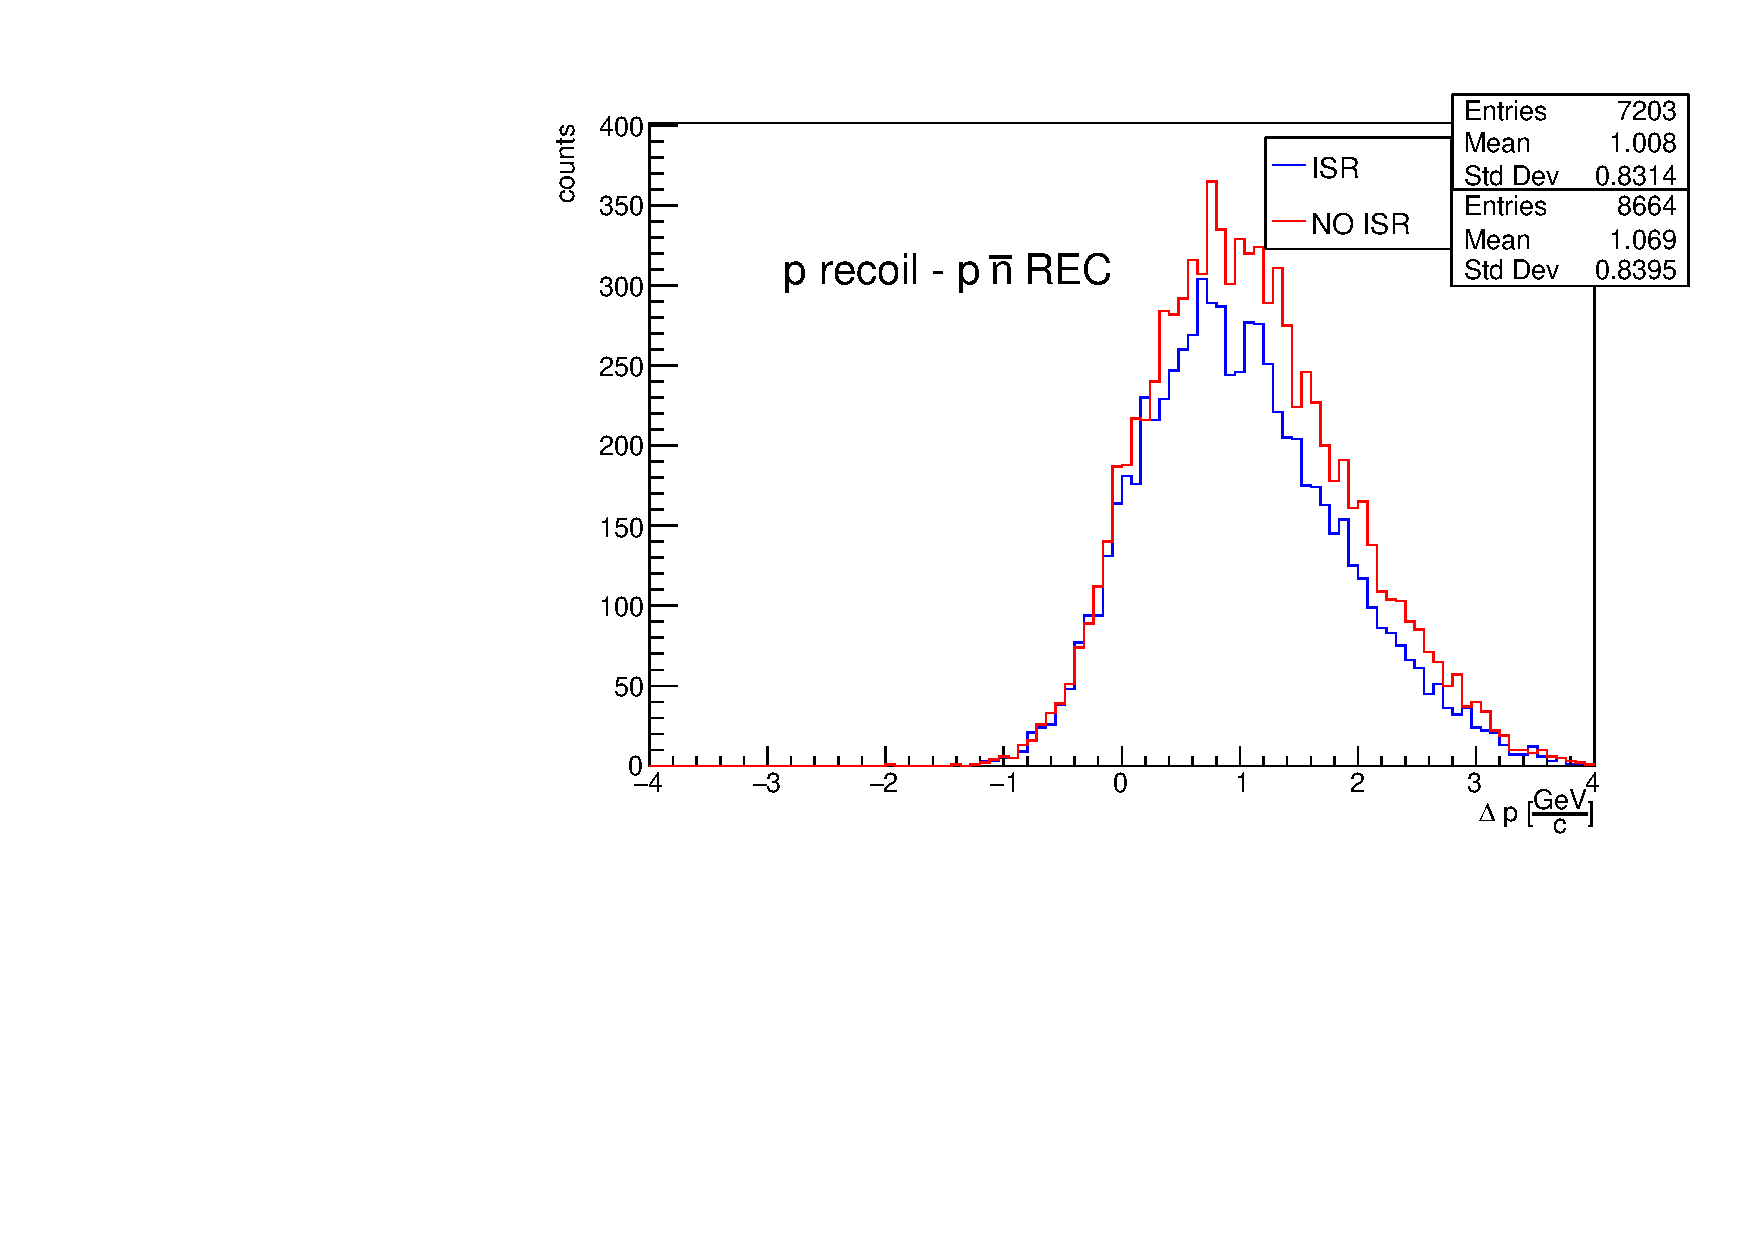
\includegraphics[width=0.49\textwidth]{nbar_MC/images/diff_pREC_np_rec.pdf}
     \caption{Momentum and $\theta$ angle residuals distribution between recoil system and anti-neutron candidate}
\end{figure}

Besides exhibiting poor resolution, the reconstructed momentum of the $\bar{n}$ is underestimated as the residuals distributions show, suggesting a missing energy in the shower. Therefore, the $\bar{n}$ momentum is poorly reconstructed using only the ECL information. Most of anti-neutrons undergo in annihilation with hadrons such as $\bar{n} n$ and $\bar{n} p$, producing pions which escape the calorimeter. Therefore, the reconstructed momentum (or energy) in the calorimeter is not directly comparable with the one of anti-neutrons.
$\\$
\subsection{The $\bar{n}$ ancestors analysis}
As observed, cluster split-off and/or pre-showering effects can occur distorting the $\bar{n}$ reconstructed distributions. 
$\\$
Since the ISR and NO ISR results are analogous, only the ISR case are analyzed on the following section for smoother reading.

 \begin{figure}[H]
    \centering
     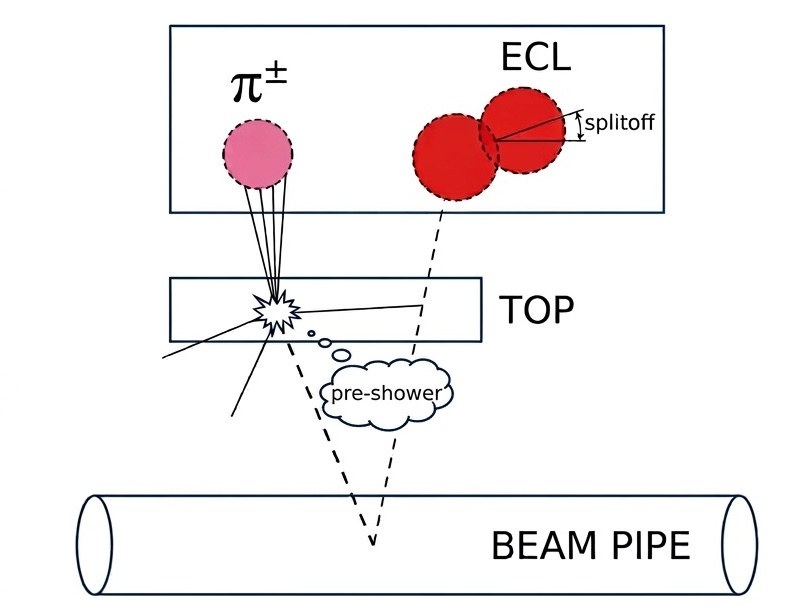
\includegraphics[width=0.55\textwidth]{nbar_MC/images/spoff_pshow}
     \caption{Artistic sketch displaying cluster split-off and pre-showering effects following $\bar{n}$ annihilation. Cluster split-off occurs in the ECL, while pre-showering takes place in the TOP; the respective products then travel toward the ECL and then mis-identified as the primary cluster associated to the anti-neutron}
\end{figure}

The secondary particle from $\bar{n}$ annihilation can be detected as the primary ECL cluster, resulting in information loss and requiring the TOP time information to improve the anti-neutron detection. 
\subsubsection{The ancestor meta-variables}
In order to study the chain and the kinship degree of the neutral cluster associated to $\bar{n}$ candidates detected in the ECL, the basf2 \textbf{ancestor} meta-variables are analyzed, such as:

\begin{itemize}
\item \textbf{varForFirstMCAncestorOfType(type, variable)}: this metavariable returns the requested \textbf{variable} of the first ancestor of the given \textbf{type}  -a specific particle- found in a certain point of the chain

\item \textbf{hasAncestor(PDG, abs)}: this metavariable returns a positive integer if an ancestor -a certain relatives in the cahin- with the given \textbf{PDG} code is found, 0 otherwise. It means thats 1 = first mother, 2 = grandmother, etc. Second argument \textbf{abs} is optional: 1 means that the sign of the PDG code is taken into account, default is 0
\end{itemize}

A typical scenarios of $\bar{n}$ as ancestor could  be the following:
\begin{center}
0)$\bar{n}$ from IP $\rightarrow$ 1)$\bar{n}$ annihilation in TOP (pions produced) $\rightarrow$ 2) pions detected 
0)$\bar{n}$ from IP $\rightarrow$ 1)$\bar{n}$ annihilation in ECL (pions produced) $\rightarrow$ 2) pions detected
\end{center}

Therefore the variables \textbf{varForFirstMCAncestorOfType(anti-n0, p)} and \textbf{hasAncestor(-2112, 1)} of neutral cluster associated to $\bar{n}$ are discussed. Given the close similarity between the results, only the ISR case is discussed. The hasAncestor distribution is shown below:
 \begin{figure}[H]
    \centering
     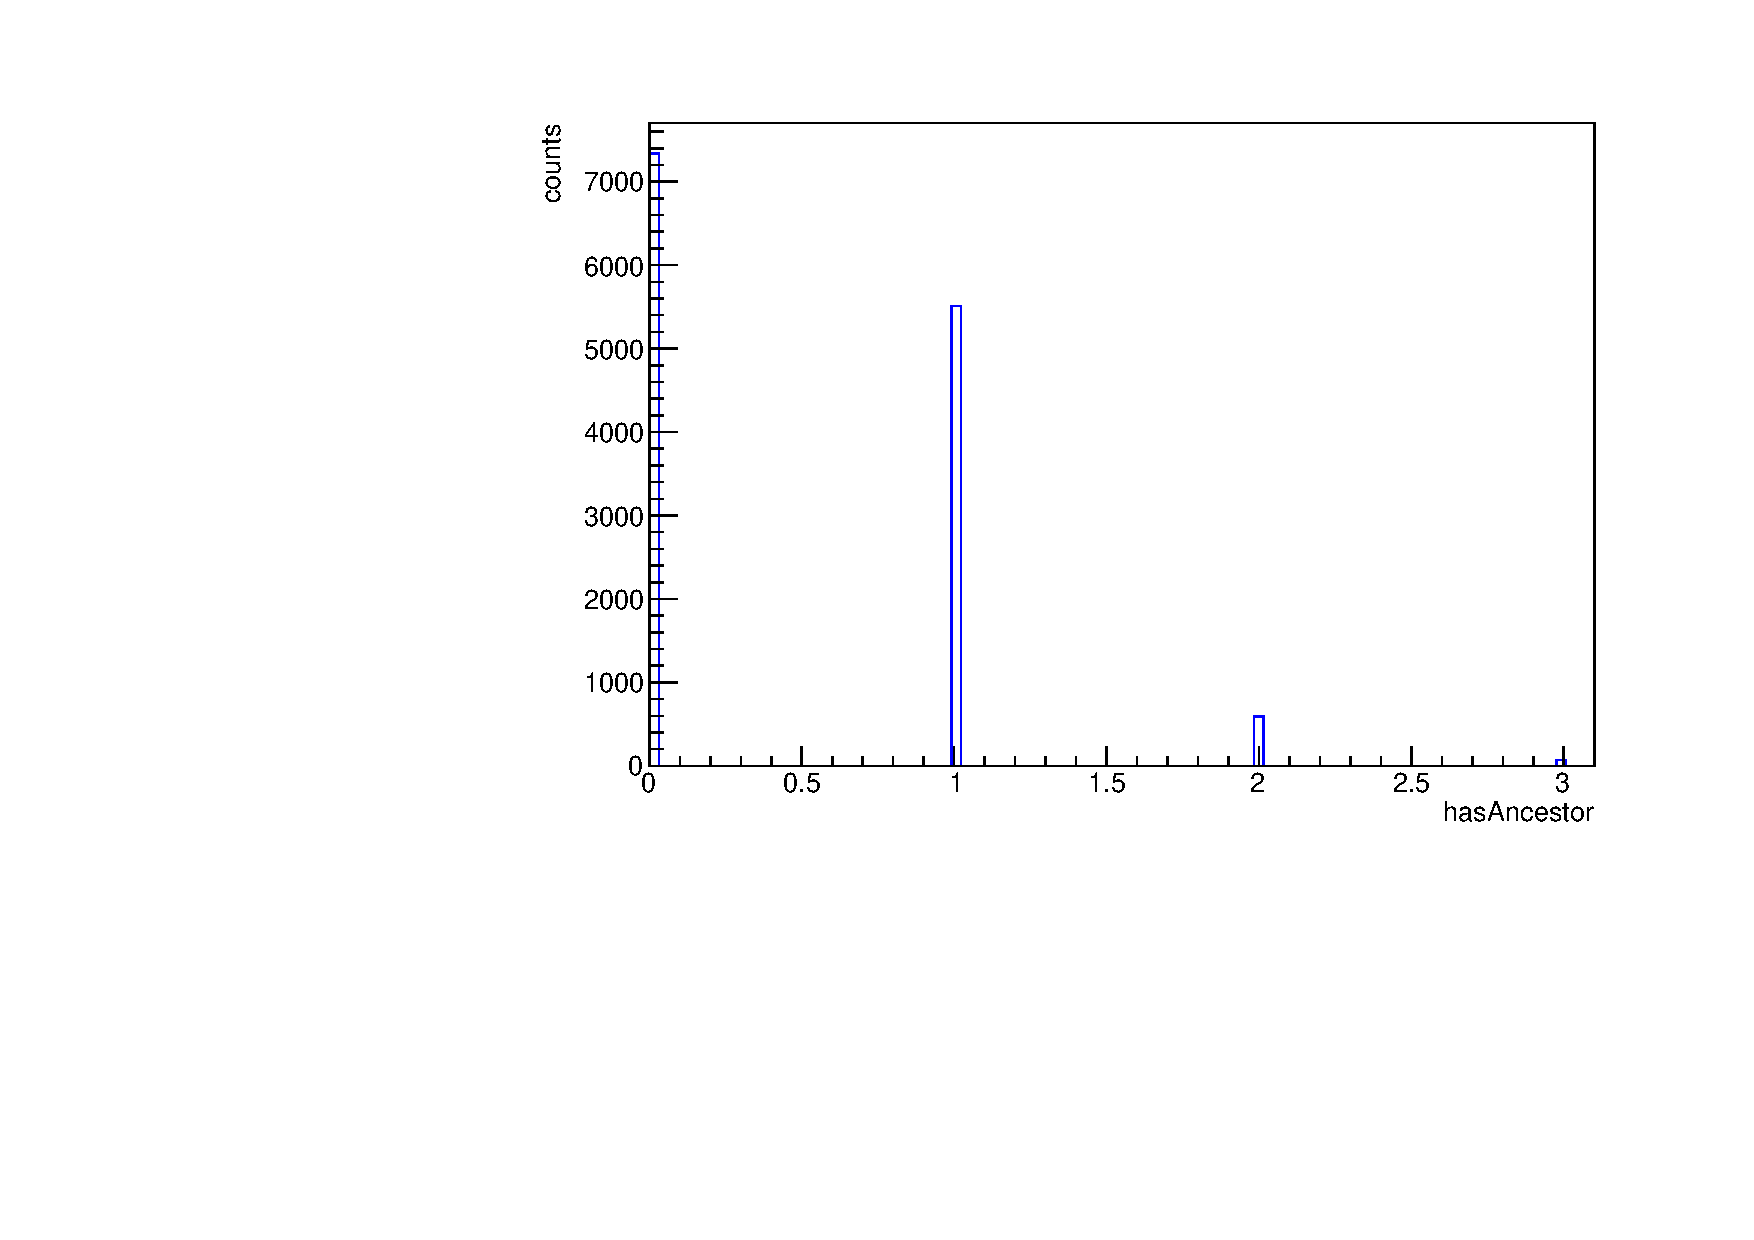
\includegraphics[width=0.70\textwidth]{nbar_MC/images/hasAncestor.pdf}
     \caption{Distribution of the ancestry kinship degree of anti-neutron candidates with an anti-neutron present in their ancestry chain}
\end{figure}

Consequently, most $\bar{n}$ candidates lack an $\bar{n}$ in their relative chain (has\_Ancestor=0), suggesting they are the primary $\bar{n}$ themselves. The second contribution is made of $\bar{n}$ candidates having $\bar{n}$ as mother etc. 
$\\$
In order to directly study the contribution of each term, it could be useful to access to the Monte Carlo truth and look at the PID trough the \textbf{mc\_PDG}, which basically is the real PDG of the selected candidates coming from the generator. The obtained distributions are shown below:

 \begin{figure}[H]
    \centering
    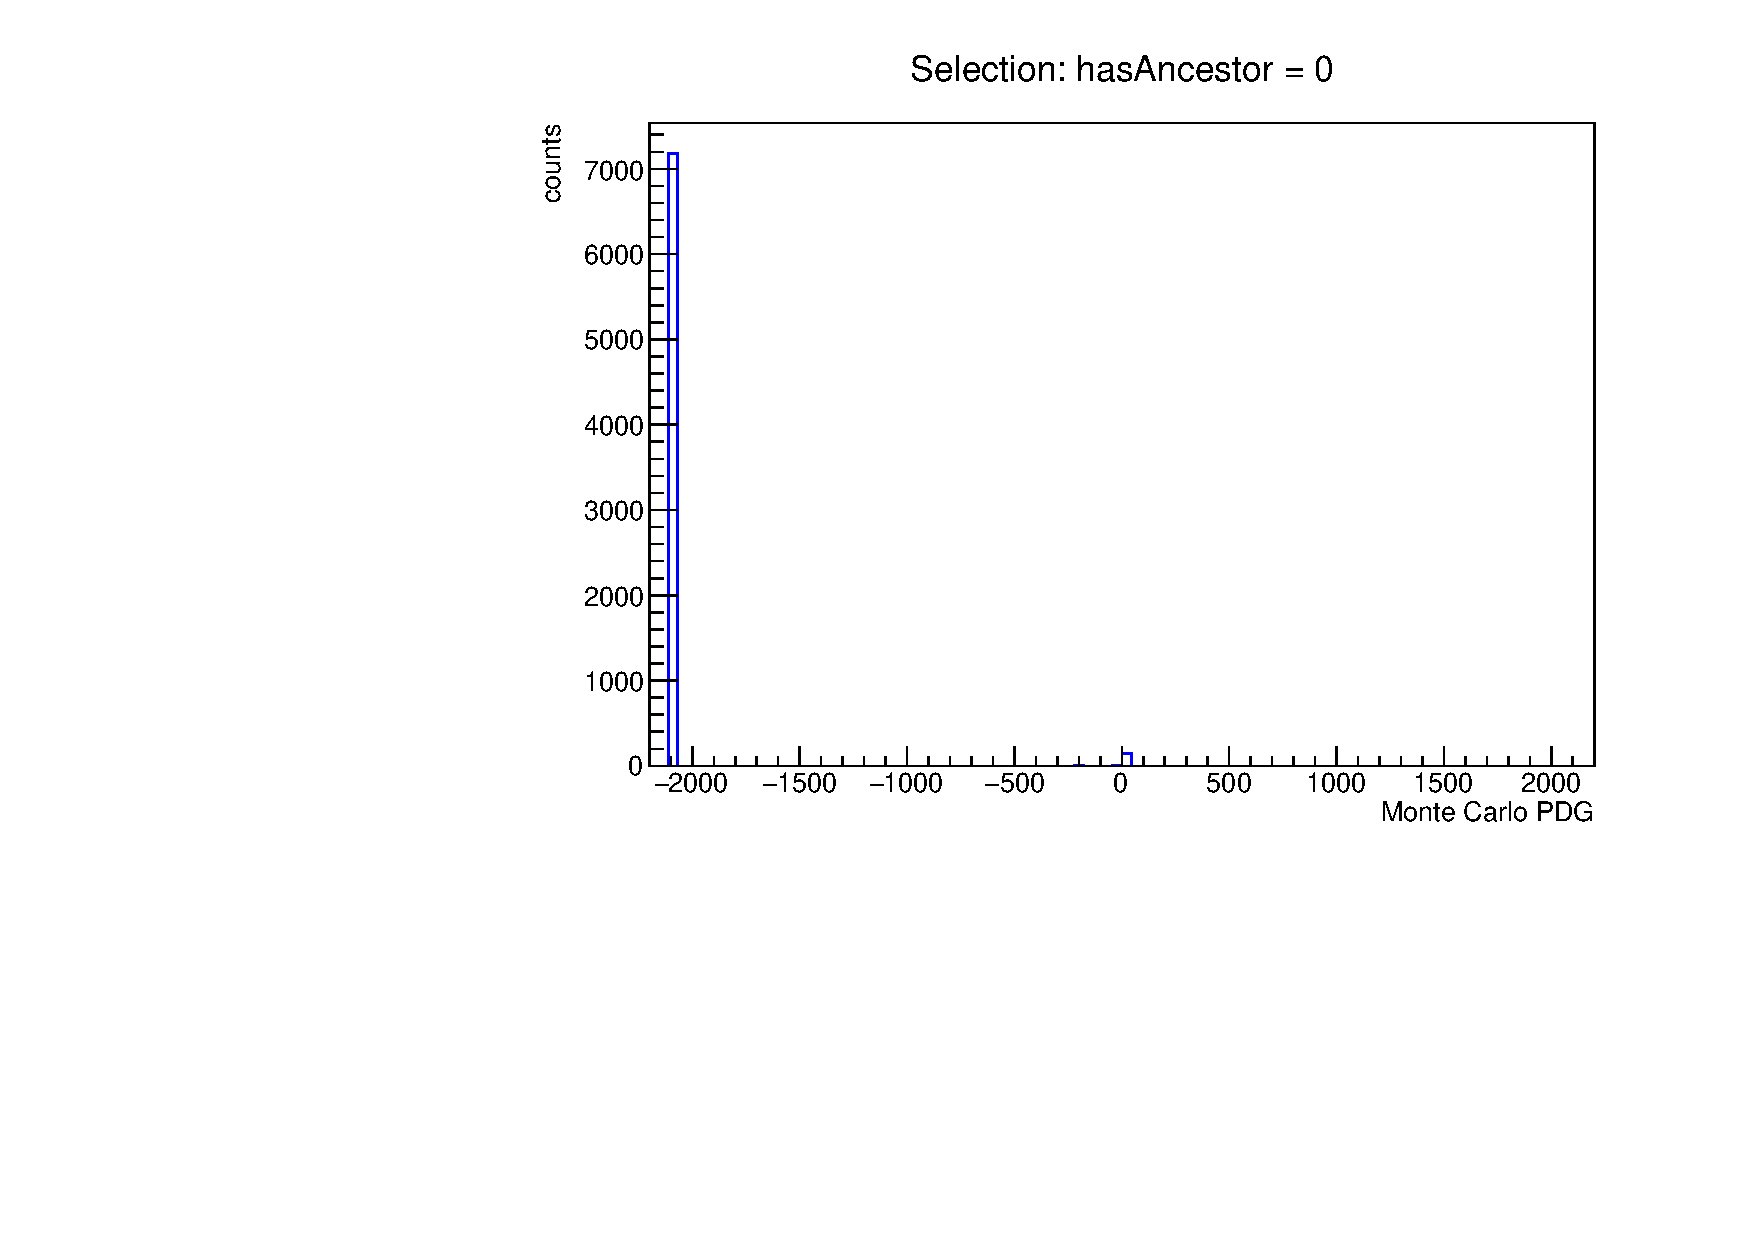
\includegraphics[width=0.49\textwidth]{nbar_MC/images/mc_pdg_hasAncestor=0.pdf}
    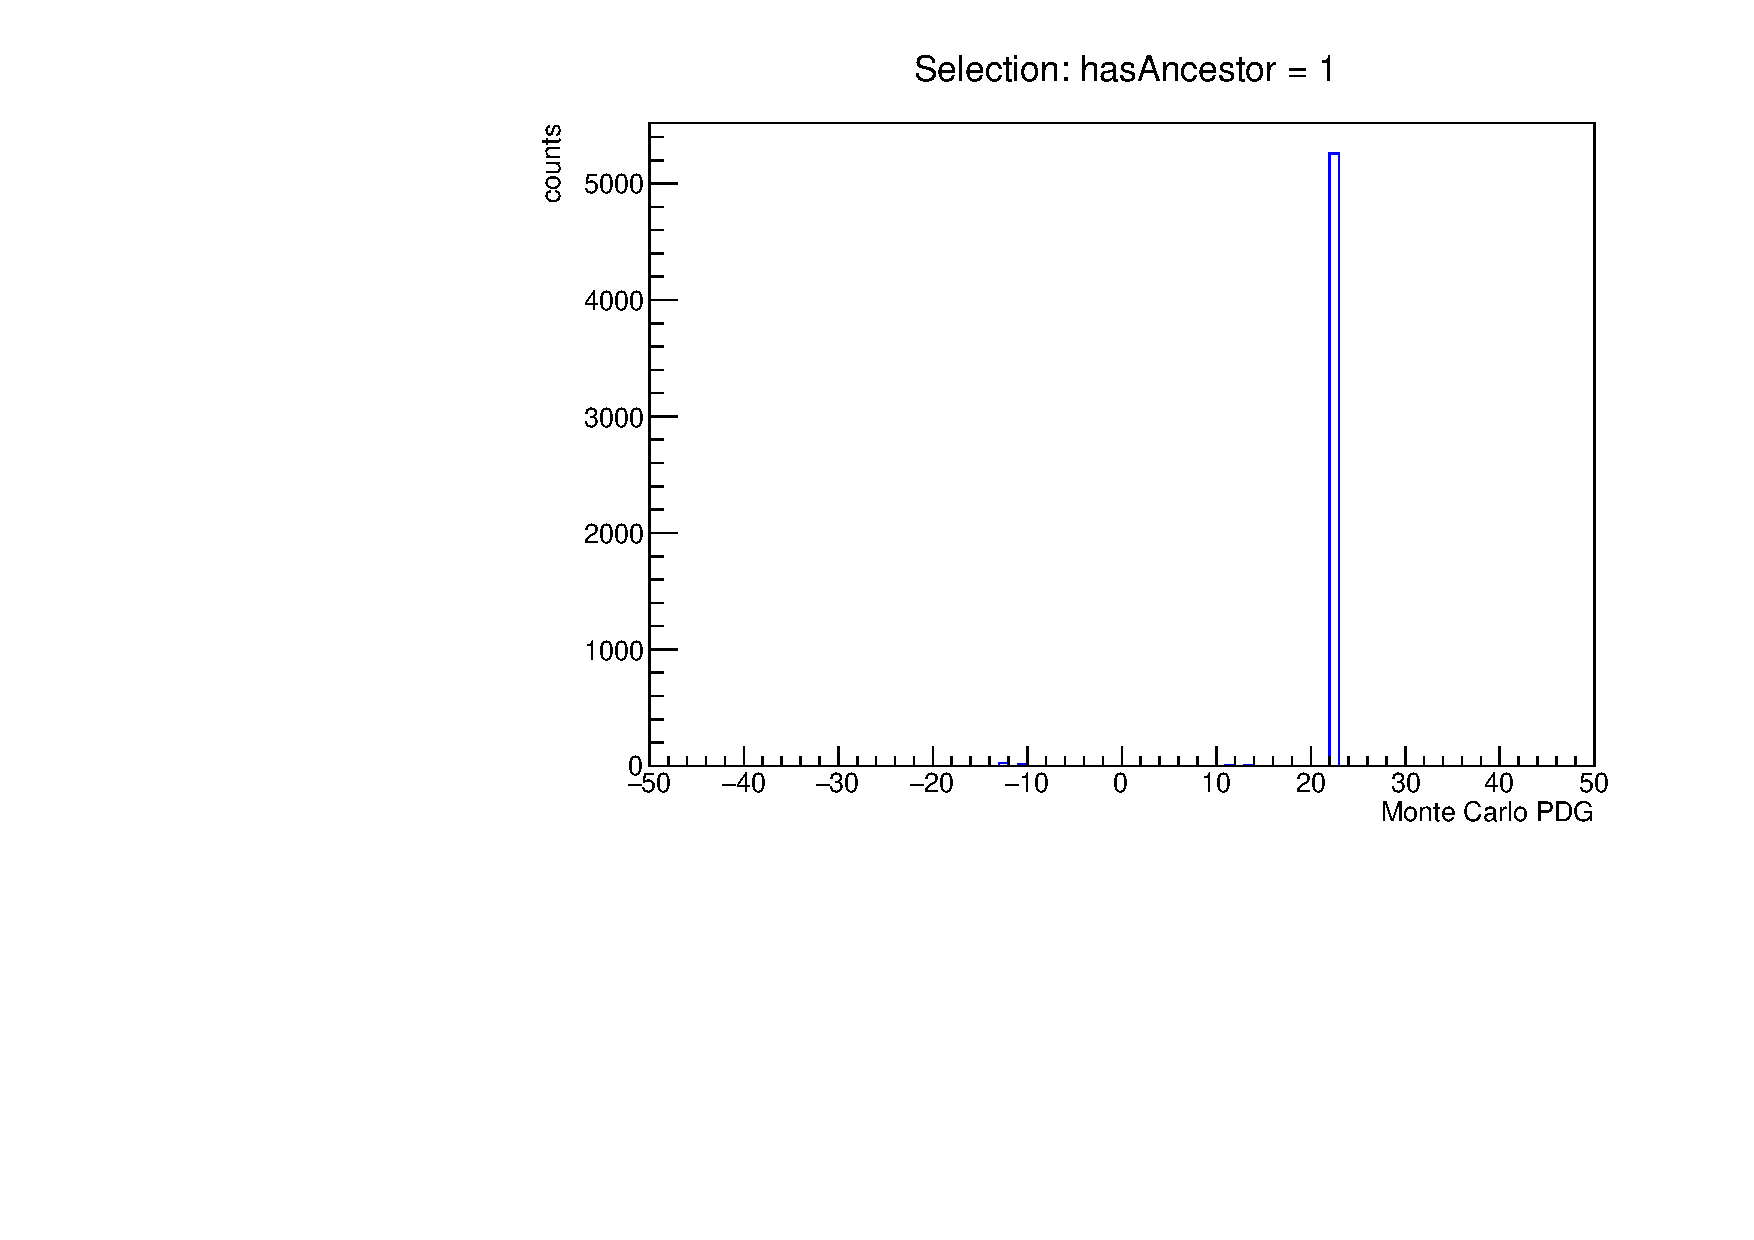
\includegraphics[width=0.49\textwidth]{nbar_MC/images/mc_pdg_hasAncestor=1.pdf}
     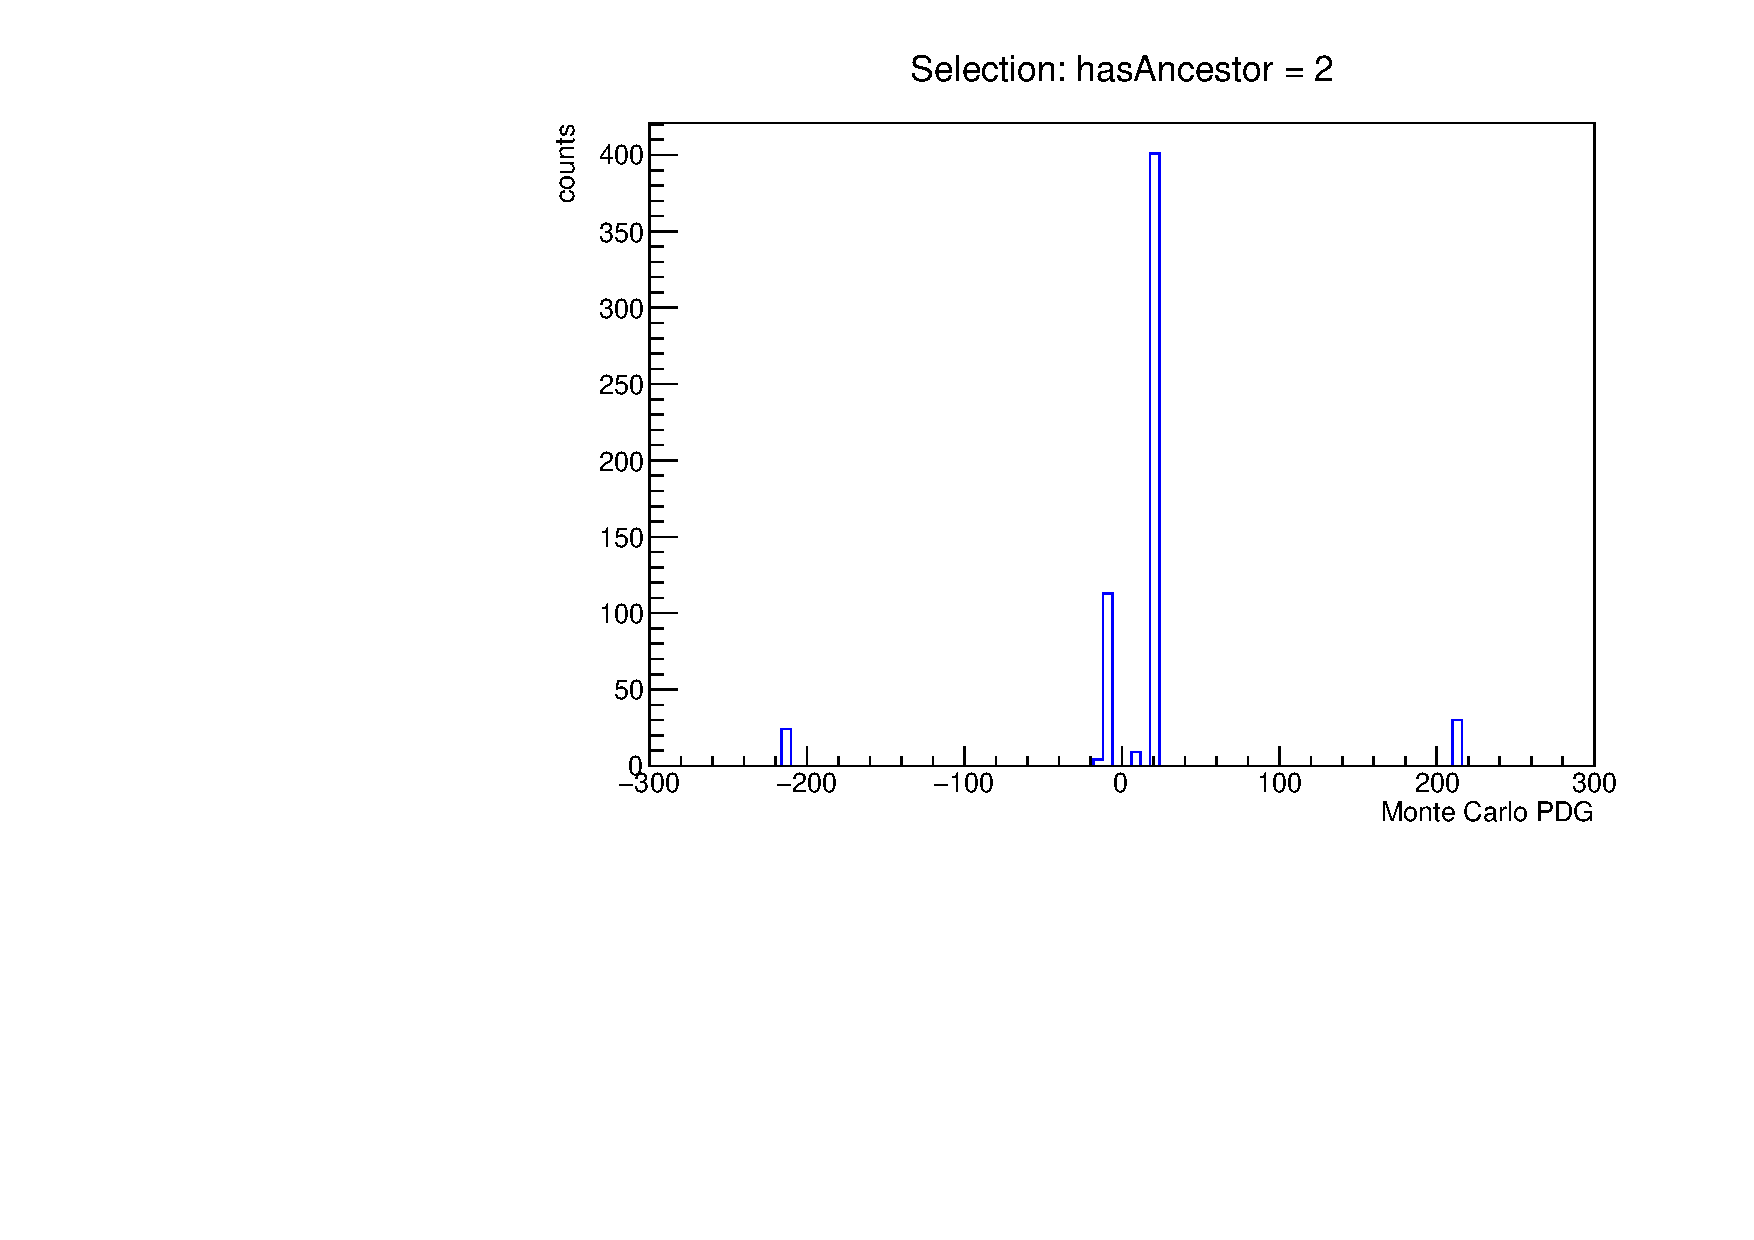
\includegraphics[width=0.49\textwidth]{nbar_MC/images/mc_pdg_hasAncestor=2.pdf}
     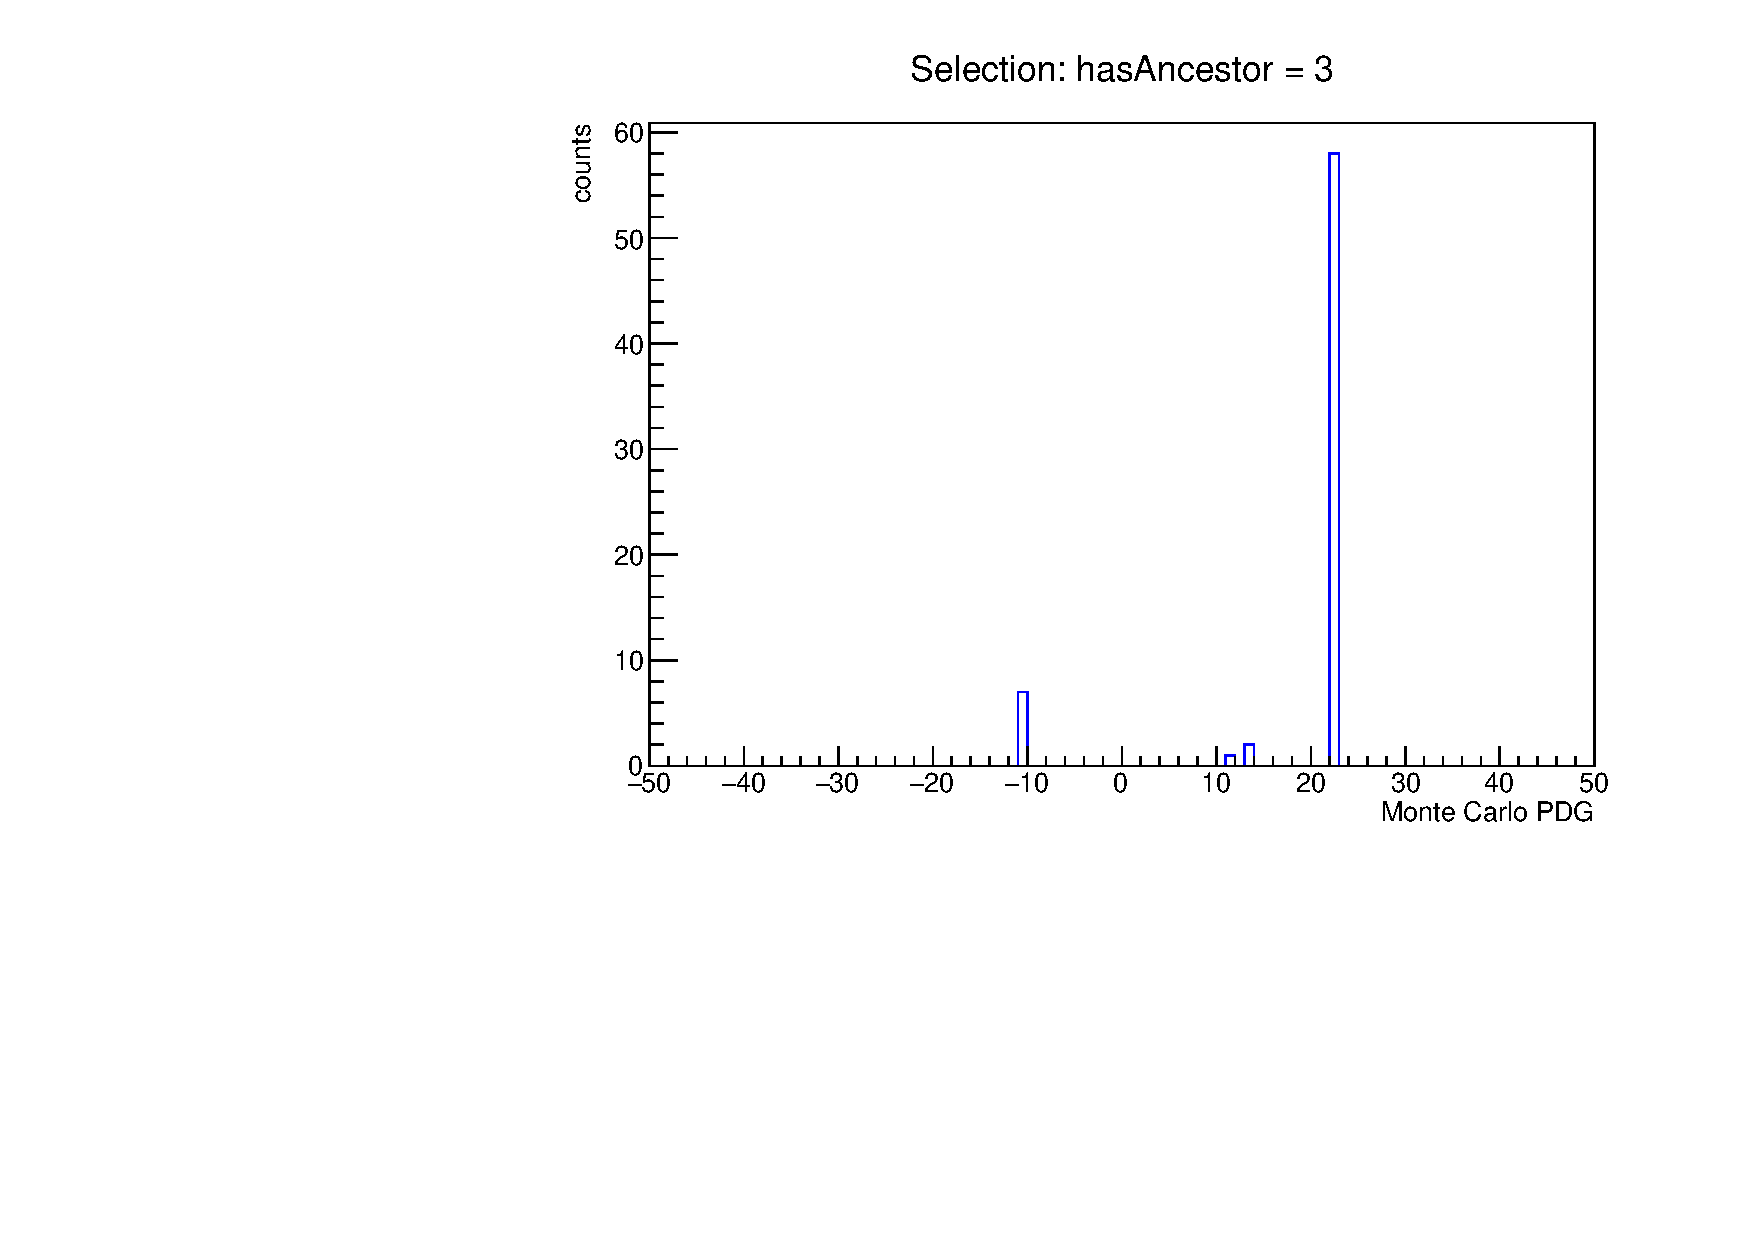
\includegraphics[width=0.49\textwidth]{nbar_MC/images/mc_pdg_hasAncestor=3.pdf}
     \caption{Monte Carlo PDG codes of candidates with degrees of ancestry selection. As mentioned, the MC PDG variable reveals the generator-level identity of the reconstructed particle by providing its PDG code}
\end{figure}

\begin{itemize}
\item \textbf{hasAncestor = 0} clearly shows that $\bar{n}$ candidates without an $\bar{n}$ as relatives are mainly true anti-neutrons, as their Monte Carlo PDG code is primarily -2112.This is consistent since the anti-neutron comes from the IP and it is directly detected in the ECL through its own annihilation
\item \textbf{hasAncestor = 1}  shows that the $\bar{n}$ candidates with an $\bar{n}$ as mother are predominately gammas (Monte Carlo PDG = 22), suggesting they result from $\bar{n}$ interactions prior to $\bar{n}$ candidate  ECL cluster formation
\item \textbf{hasAncestor = 2} suggests that the $\bar{n}$ candidates with an $\bar{n}$ as grandmother are mainly gammas, with some spurious pions (-211 \& +211) and electrons or positrons (+11 \& -11). The case with hasAncestor = 3 yields analogous results
\end{itemize}

\subsubsection{Ancestor momentum}
The figure ~\ref{fig:pRecoil_nmcP} can be updated, by including the momentum of the ancestors obtained with \textbf{varForFirstMCAncestorOfType(anti-n0, p)}. The idea is to check if the information from the first structure -the one at low value of momentum- can be recovered using the ancestors chain. The obtained distributions are shown below:

 \begin{figure}[H]
    \centering
    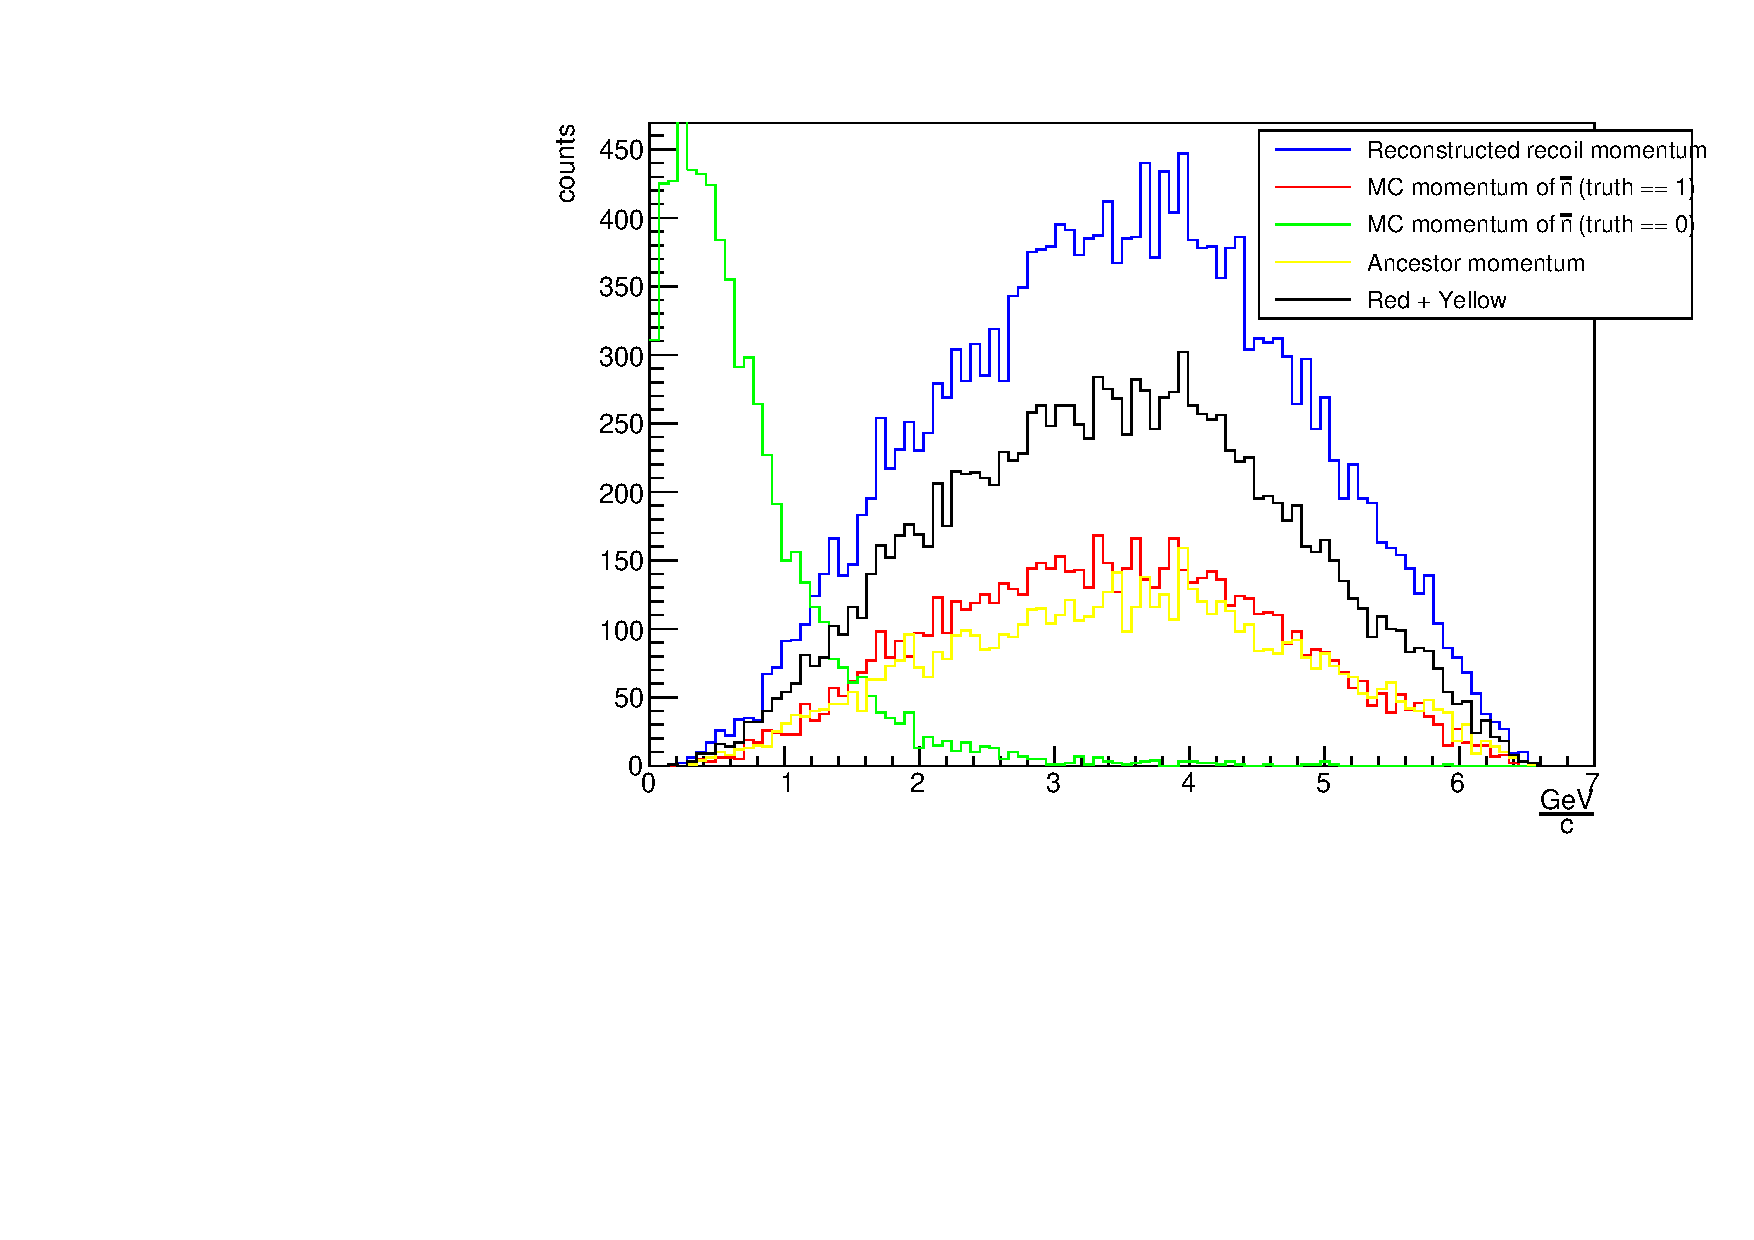
\includegraphics[width=0.7\textwidth]{nbar_MC/images/momentum_ancestors.pdf}
    \caption{Momentum comparison of different components. The recoil vector is the only reconstructed variable, while the others are obtained from Monte Carlo truth selection, as shown in the legend}
\end{figure}

The {\color{blue} blue distribution} is made of 20146 entries, the {\color{red} red one} is made of 7203 entries, the {\color{green} green one} is made of 6308 entries, the {\color{yellow} yellow one} is made of 6173 entries and the {\color{black} black one} is made of 13376 entries. It means the 98\% of the first structure is recovered by ancestor momentum, suggesting that phenomena prior to neutral cluster associated to $\bar{n}$ candidates can occur, such as cluster split-off and pre-showering.
$\\$
The quality of the ancestor momentum can be discussed by studying the residuals with respect to the reconstructed recoil momentum:
 \begin{figure}[H]
    \centering
    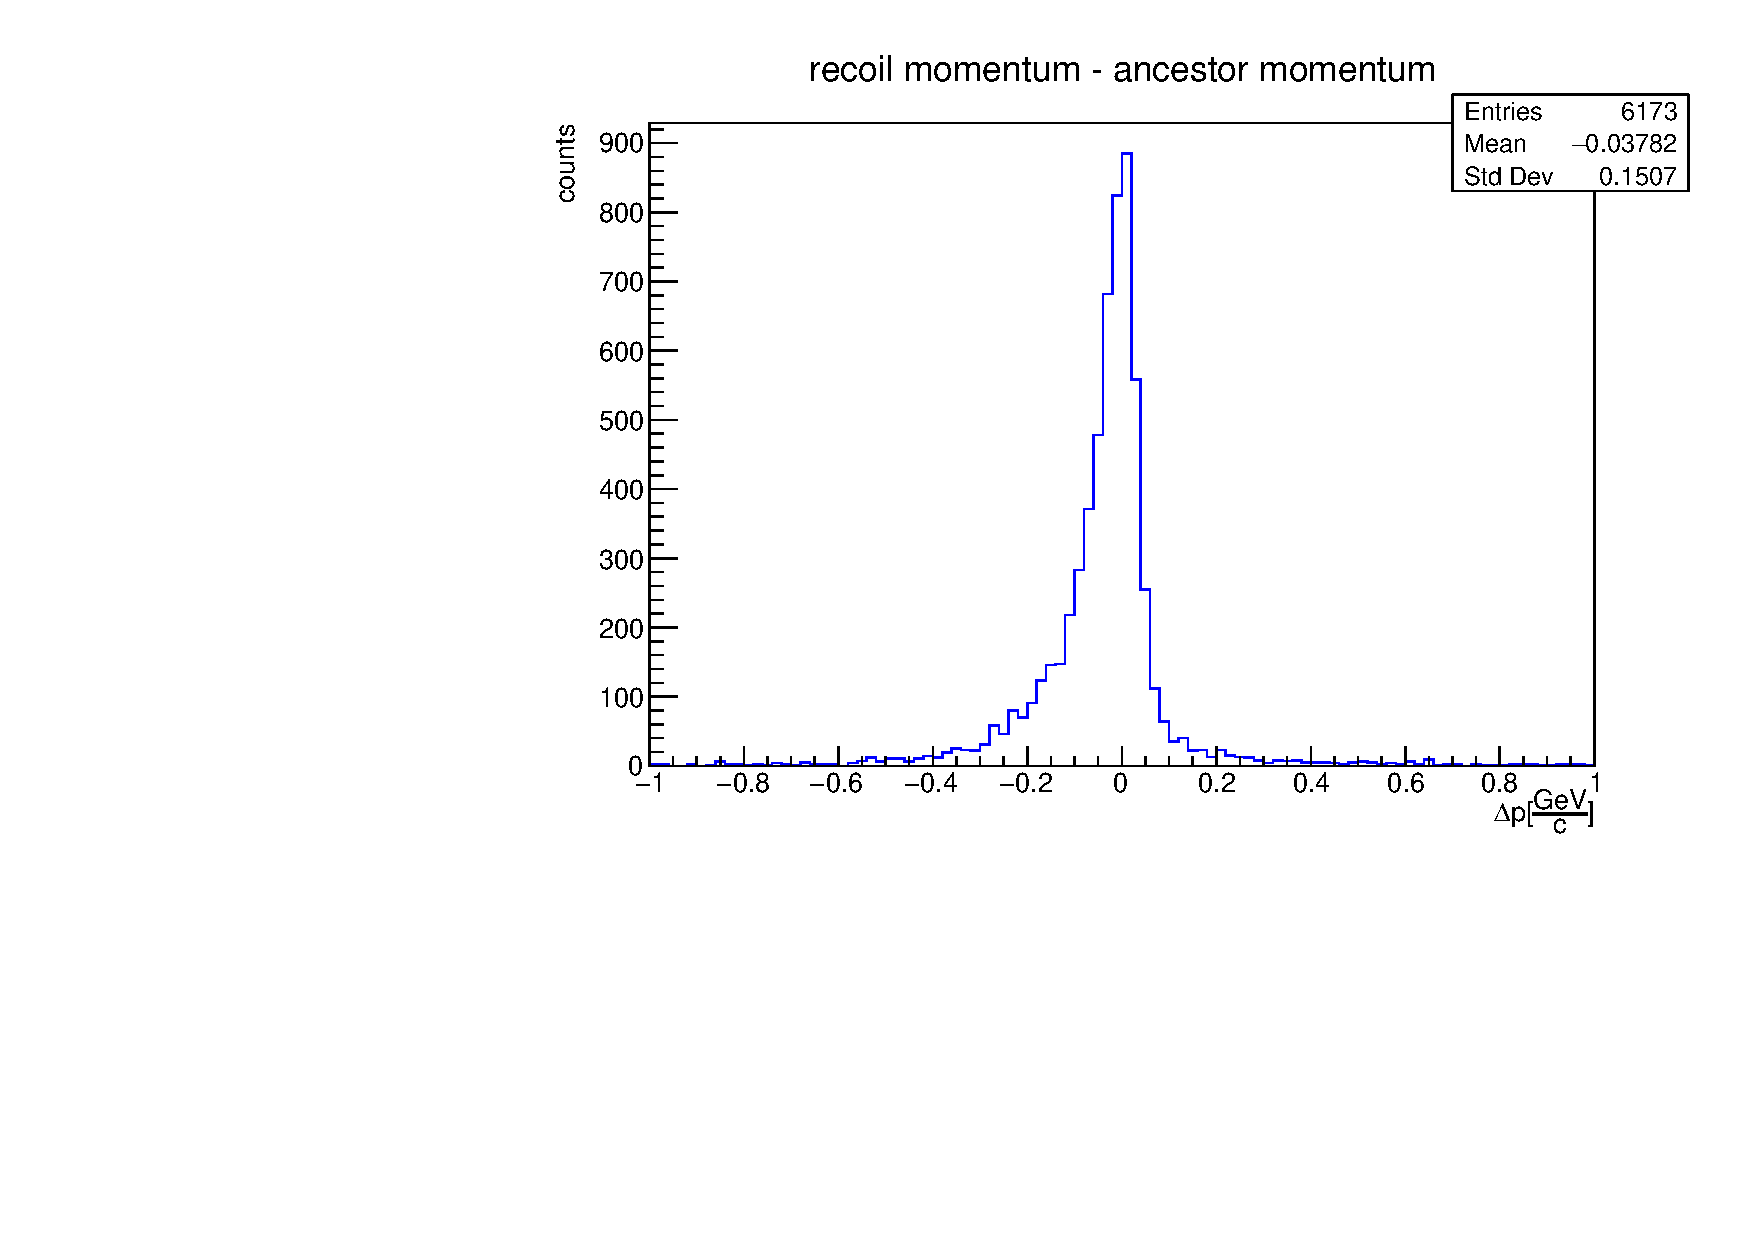
\includegraphics[width=0.7\textwidth]{nbar_MC/images/deltaP_ancestors.pdf}
    \caption{Residual distribution of ancestor momentum with respect to the recoil vector}
\end{figure}

Therefore the reconstructed recoil momentum is a good estimator of the ancestor momentum as well, confirming that cluster split-off or pre-showering may occur prior the ECL cluster formation.
$\\$
It is interesting as well to note that {\color{blue} 20146} - {\color{black} 13376} = 6779 which exactly matches the number of $\bar{n}$ candidates associated with a \textbf{NaN} value, mainly particles that did not receive a correct Monte Carlo association during MC truth matching. They cannot be recovered. The meta-variable \textbf{mcErrors} shows as a bit number the reason why the Monte Carlo fails the association. This variable explicitly shows this behavior:

 \begin{figure}[H]
    \centering
    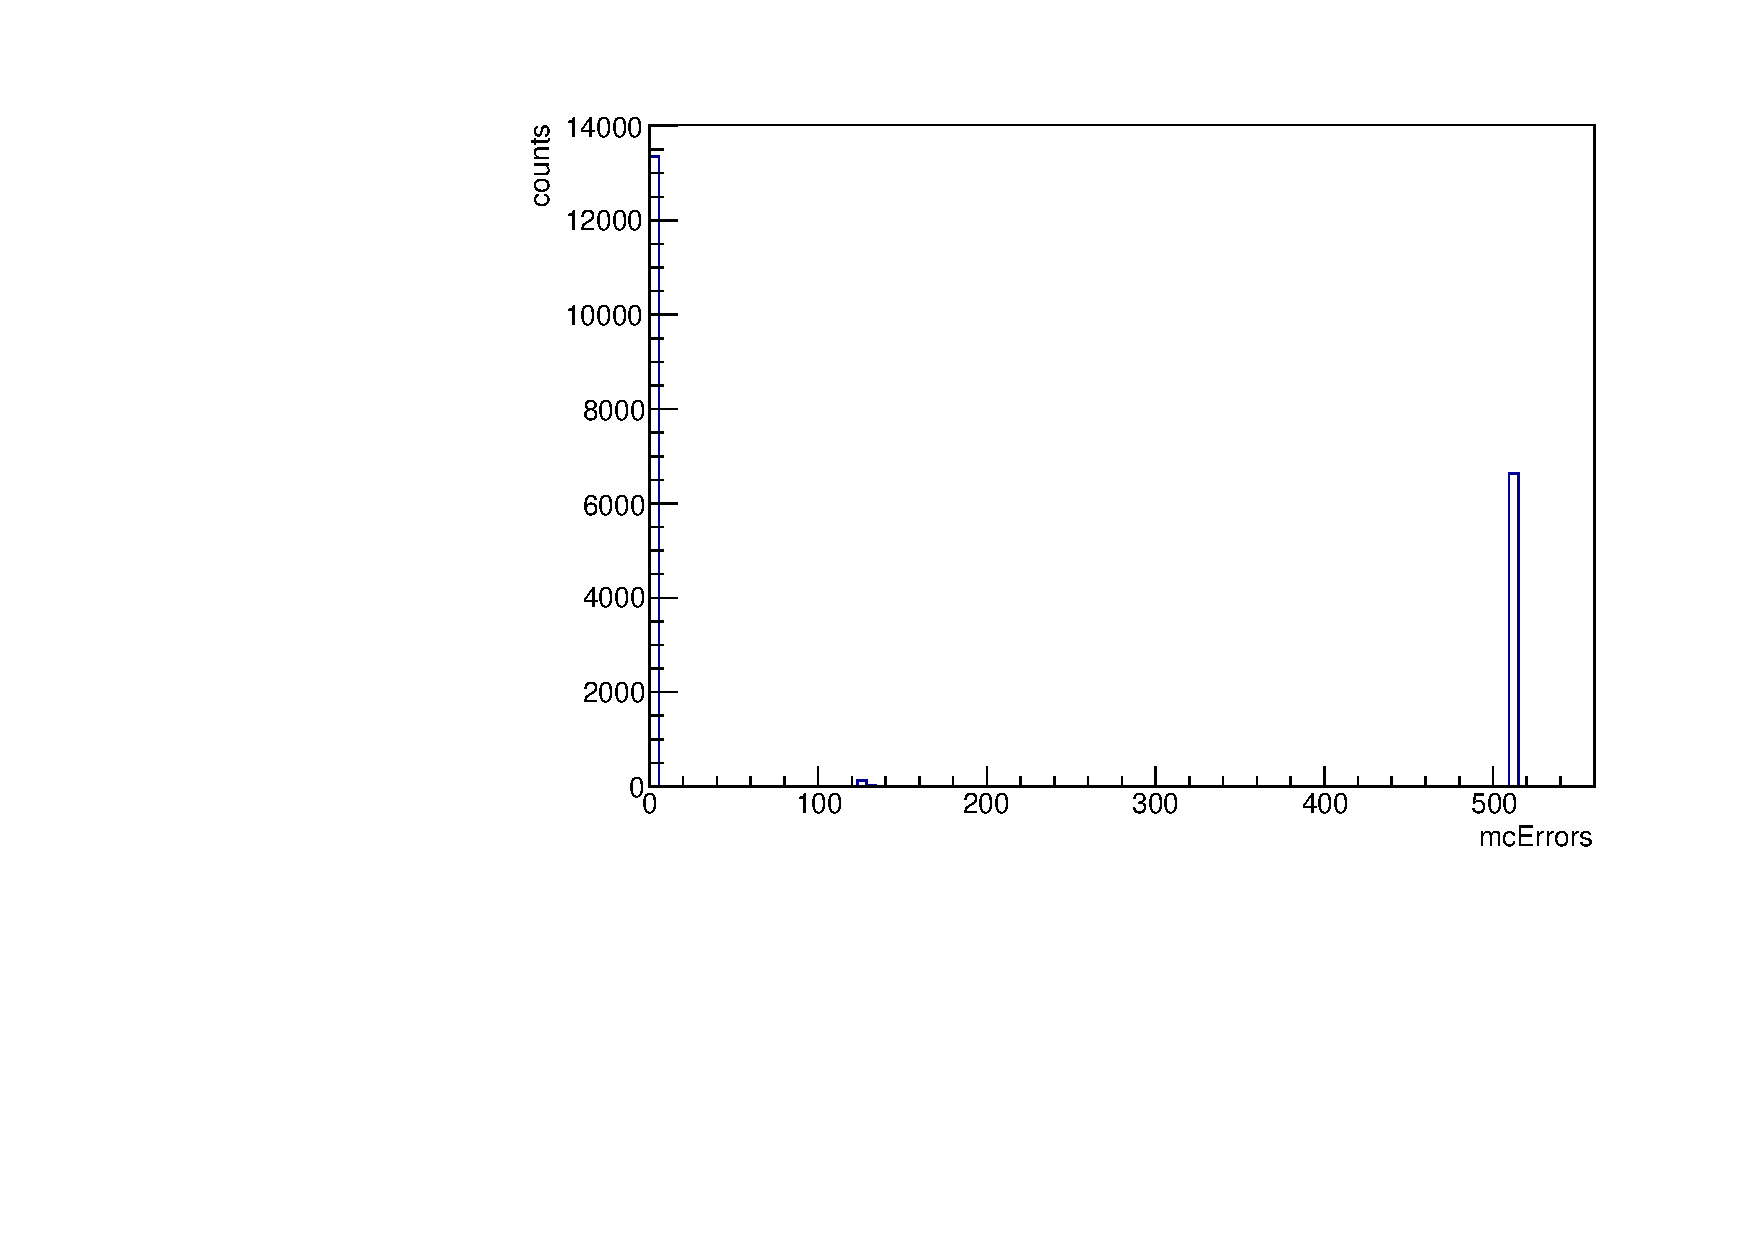
\includegraphics[width=0.7\textwidth]{nbar_MC/images/mcErrors.pdf}
\end{figure}

Where the first peak is above the code \textbf{0}, which means that "\emph{This particle and all its daughters are perfectly reconstructed}", while the second peak is above the code \textbf{512}, which confirms that "\emph{There was an error in MC matching. Not a valid match. Might indicate fake/background track or cluster}", as expected.

\subsubsection{$\bar{n}$ vertex production}
Eventually, in order to a comprehensive ancestor analysis, it could be useful to discuss the generator-level radial production distance $\rho = \sqrt{x^2 + y^2}$ -the vertex production- of $\bar{n}$ candidates, from the z-axis. 
$\\$
To provide a clear overview of $\rho$, the distribution is splitted in two parts: the left part -close to the collision diamond- ($\rho \in [0,0.1]$ cm) and the right part -far from the collision diamond- ($\rho \in (0.1,220]$ cm). The obtained result is shown below:
 \begin{figure}[H]
    \centering
    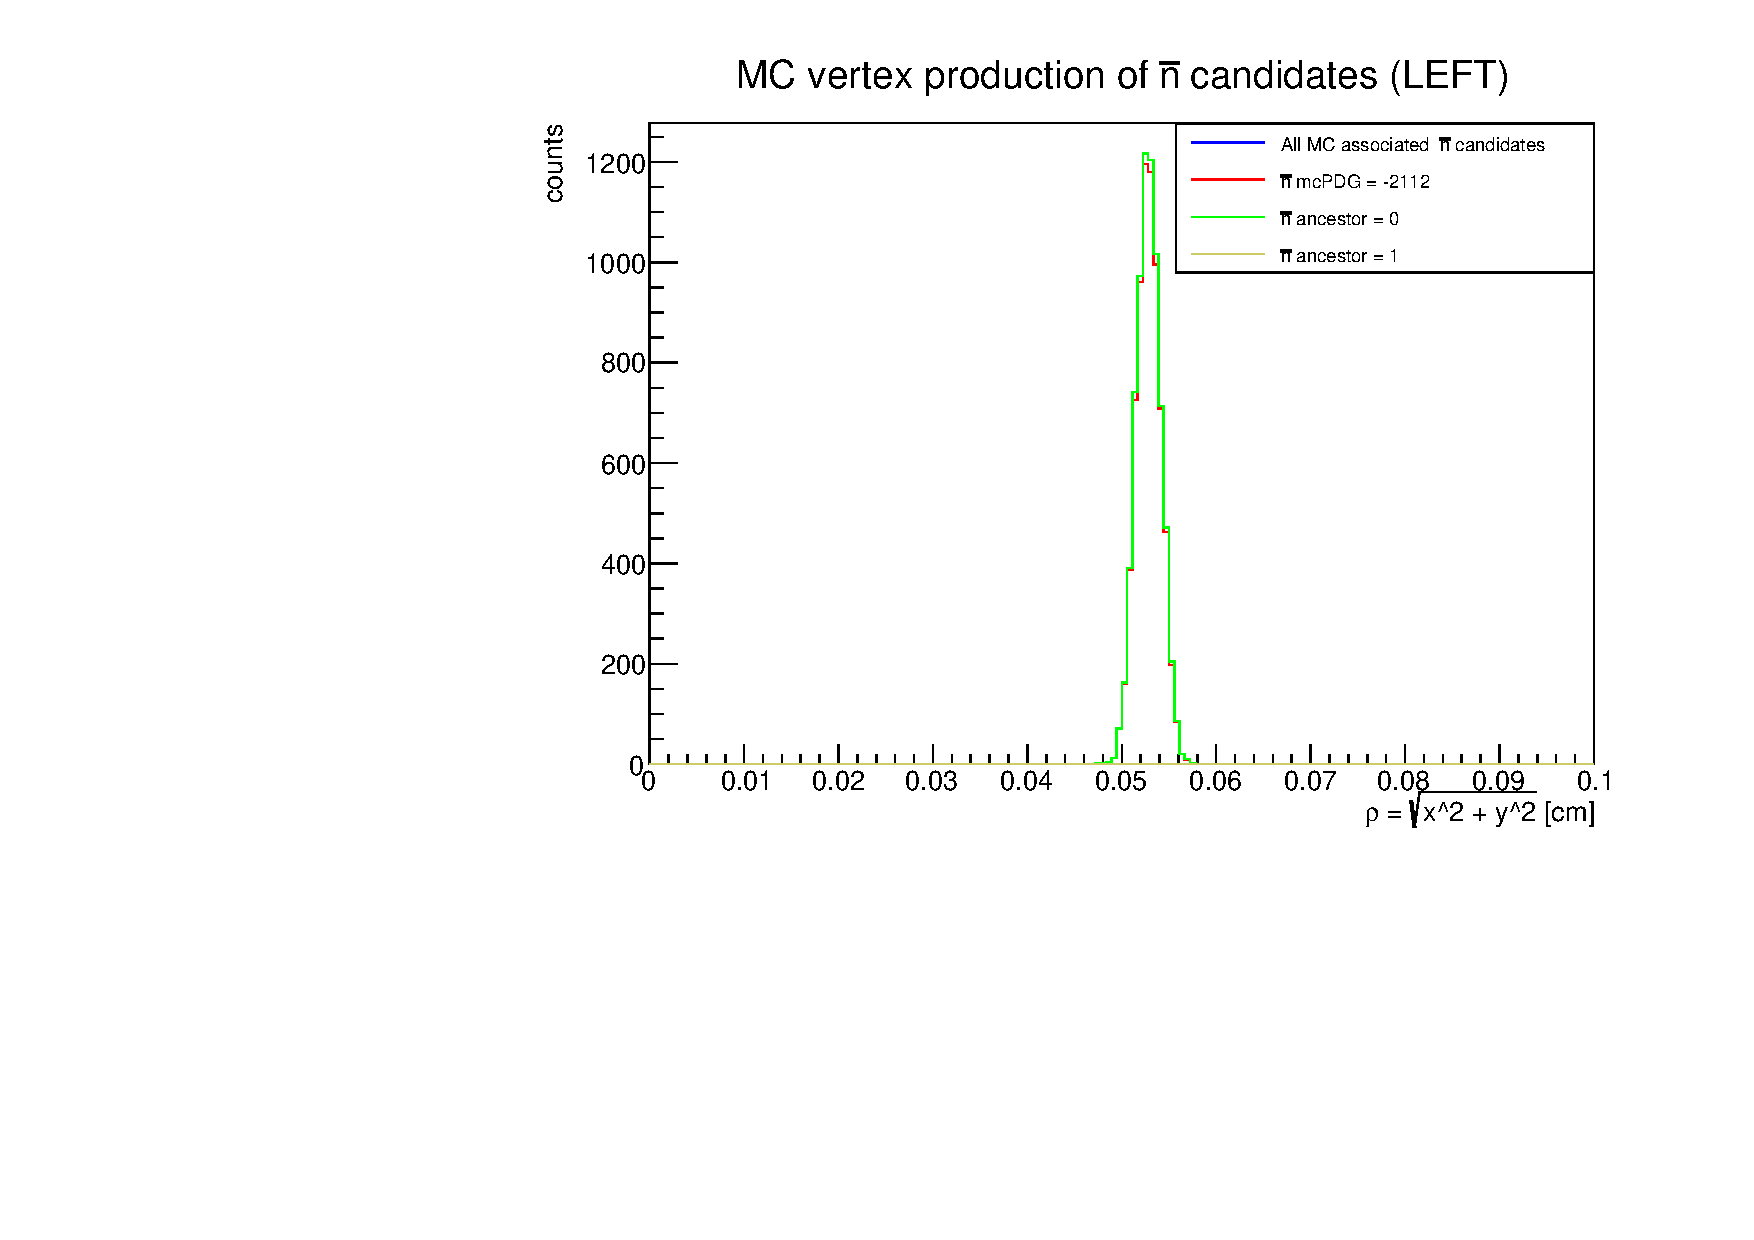
\includegraphics[width=0.49\textwidth]{nbar_MC/images/mcDistance_sx.pdf}
    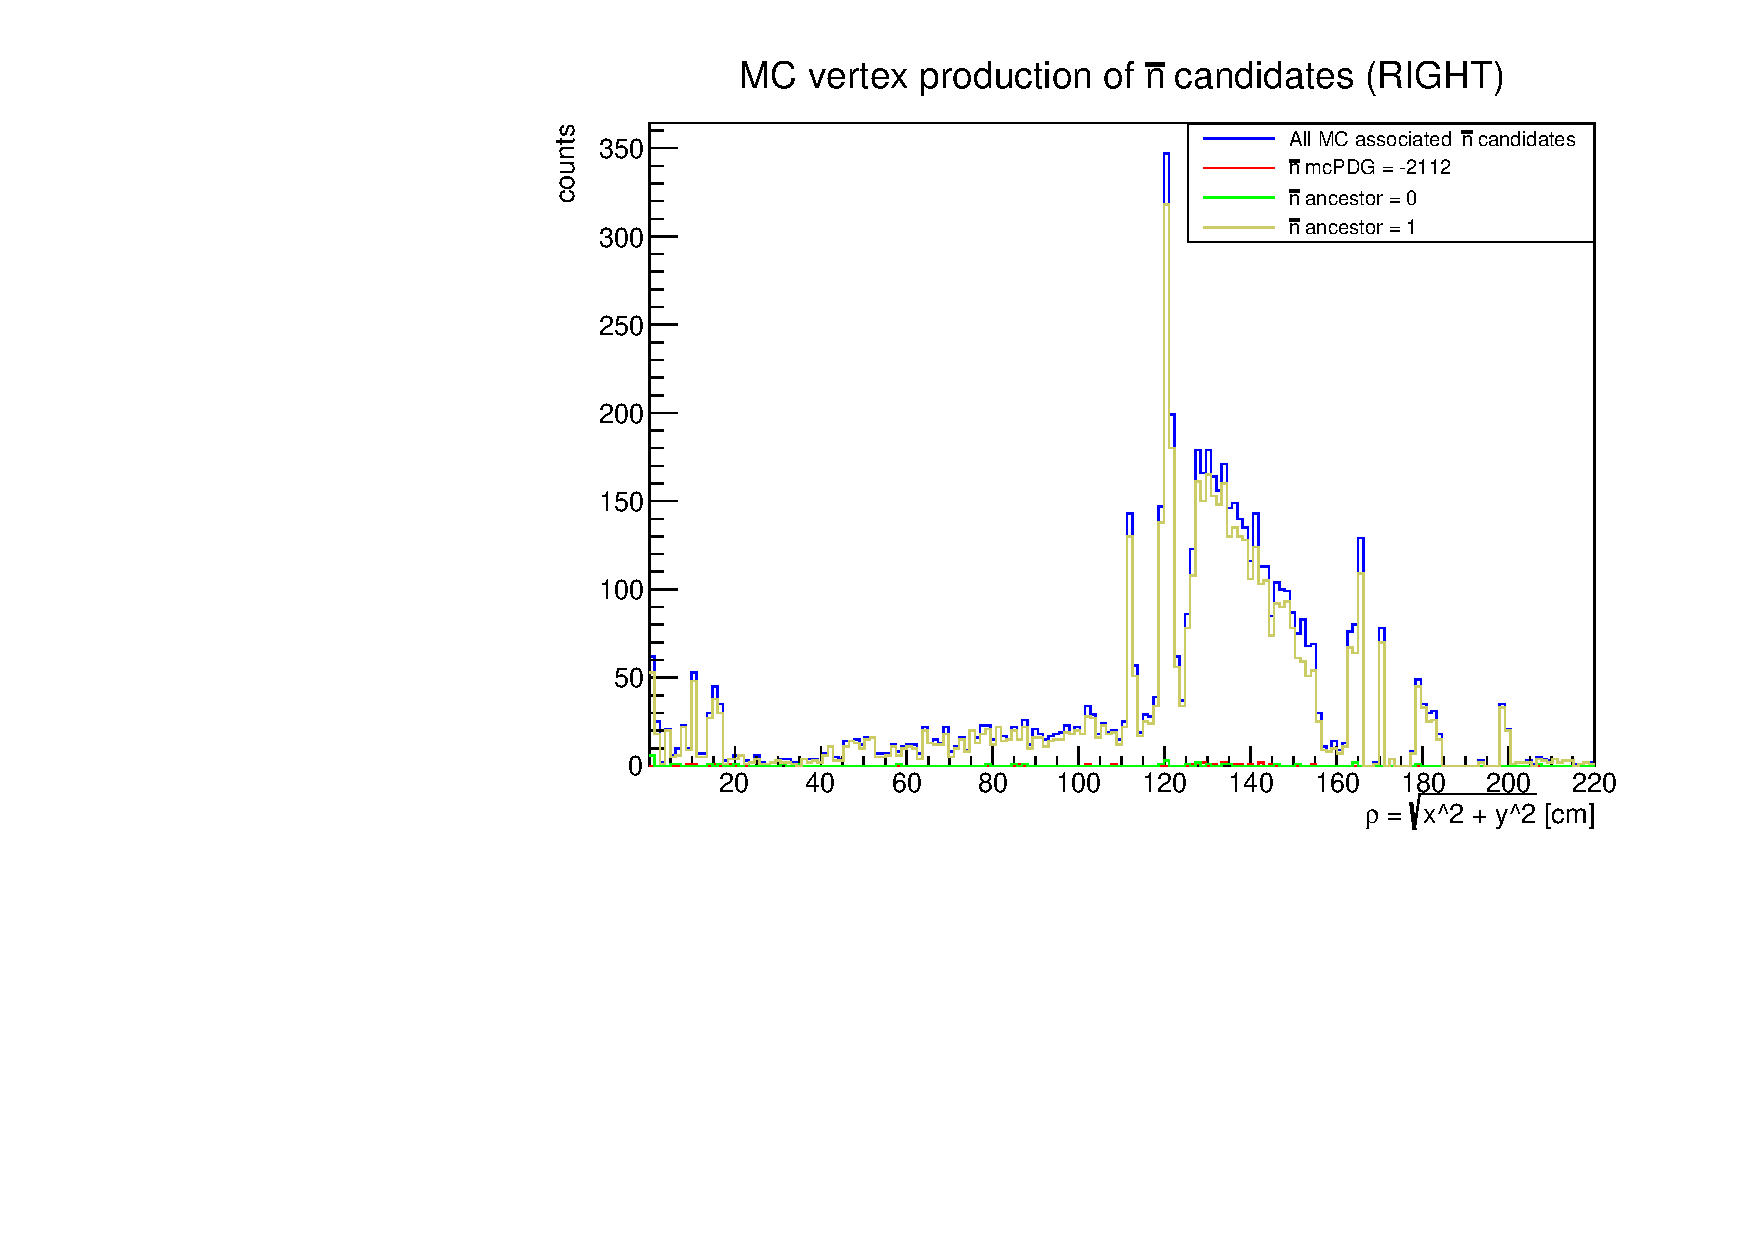
\includegraphics[width=0.49\textwidth]{nbar_MC/images/mcDistance_dx.pdf}
    \caption{$\bar{n}$ production vertex: (left) close to the IP (right) far from the IP}
\end{figure}

As expected, the correctly associated anti-neutrons ({\color{red} red distribution}) overlay the $\bar{n}$ candidates without an anti-neutron ancestor ({\color{green} green distribution}) and they are from the interaction point (left part). 
$\\$
As seen before, the $\bar{n}$ candidates with a $\bar{n}$ as mother are mainly photons and they are produced around the detector ({\color{yellow} yellow distribution}). It is interesting to note that the first structure is in the vertex detectors region ($\rho <$ 16 cm) and the two peaks located at the TOP edges, mainly around 118 cm (where the TOP begins) and 125 cm (where the TOP ends and the ECL starts), explicitly showing how cluster split-off and pre-showering events occur in the events.
$\\$
To compare the height comparison between the left and right contributes, the full distribution is shown below:
 \begin{figure}[H]
    \centering
    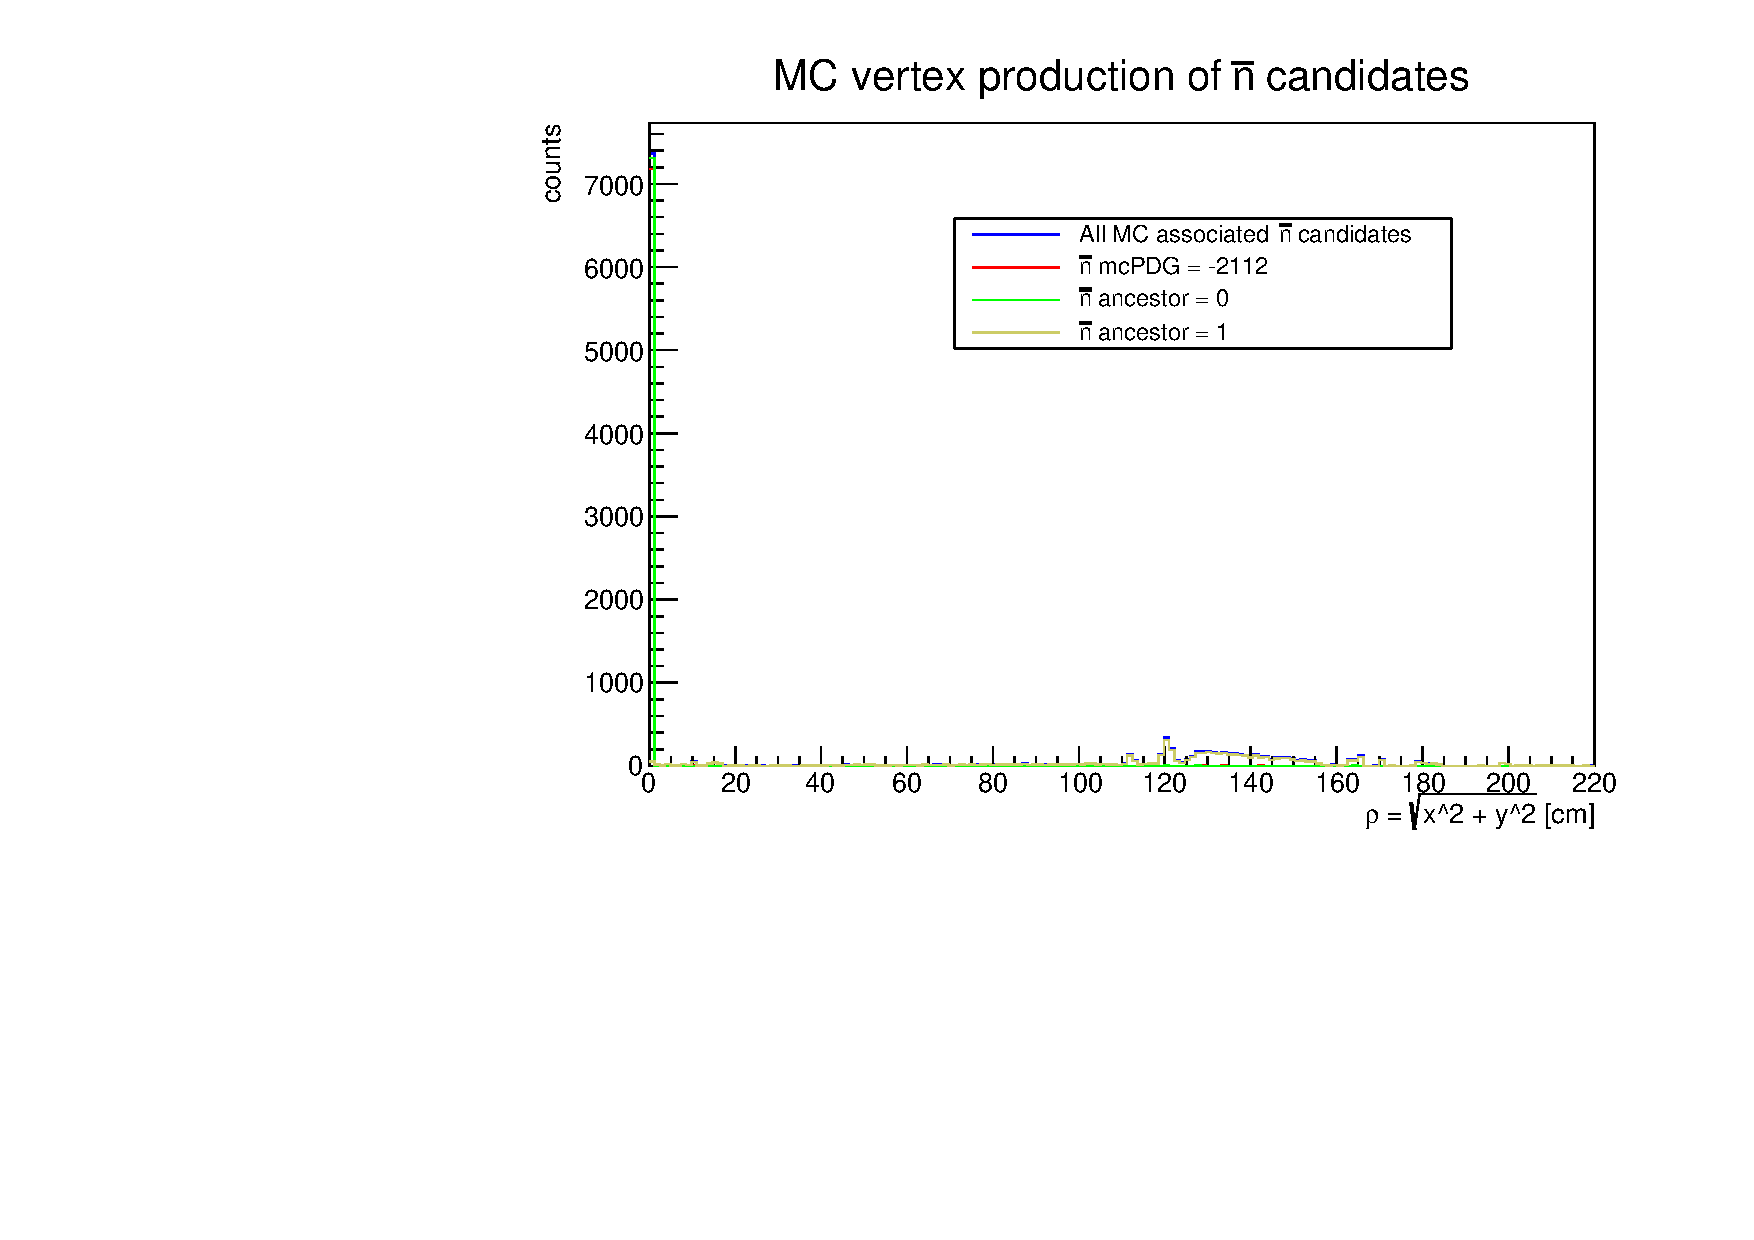
\includegraphics[width=0.70\textwidth]{nbar_MC/images/mcDistance_full.pdf}
     \caption{$\bar{n}$ production vertex showing the IP peak is the main one}
\end{figure}

\subsection{Kinematic Fit effects}
A \textbf{Kinematic Fit} is a constrained optimization technique used in particle physics to refine the measured four-momenta (or other kinematic quantities) of event particles by imposing known physical constraints, such as energy-momentum conservation or recoil mass. Measured quantities like track momenta, energies from calorimeters, or decay vertices come with resolution-limited errors from detectors. The fit adjusts these within their error bars to best satisfy the imposed constraint.
$\\$
There are several type of Kinematic Fit that could yield improved resolution. The one constraint \textbf{1C Kinematic Fit} has been tested over the $p \pi^- (\gamma_{ISR})$ system recoil mass, forcing it to the anti-neutron mass ($\sim 0.9385$ GeV) and then studying the response on the recoil kinematic variables resolution versus the anti-neutron candidate ones. The obtained residuals are shown below:

\begin{figure}[H]
    \centering
     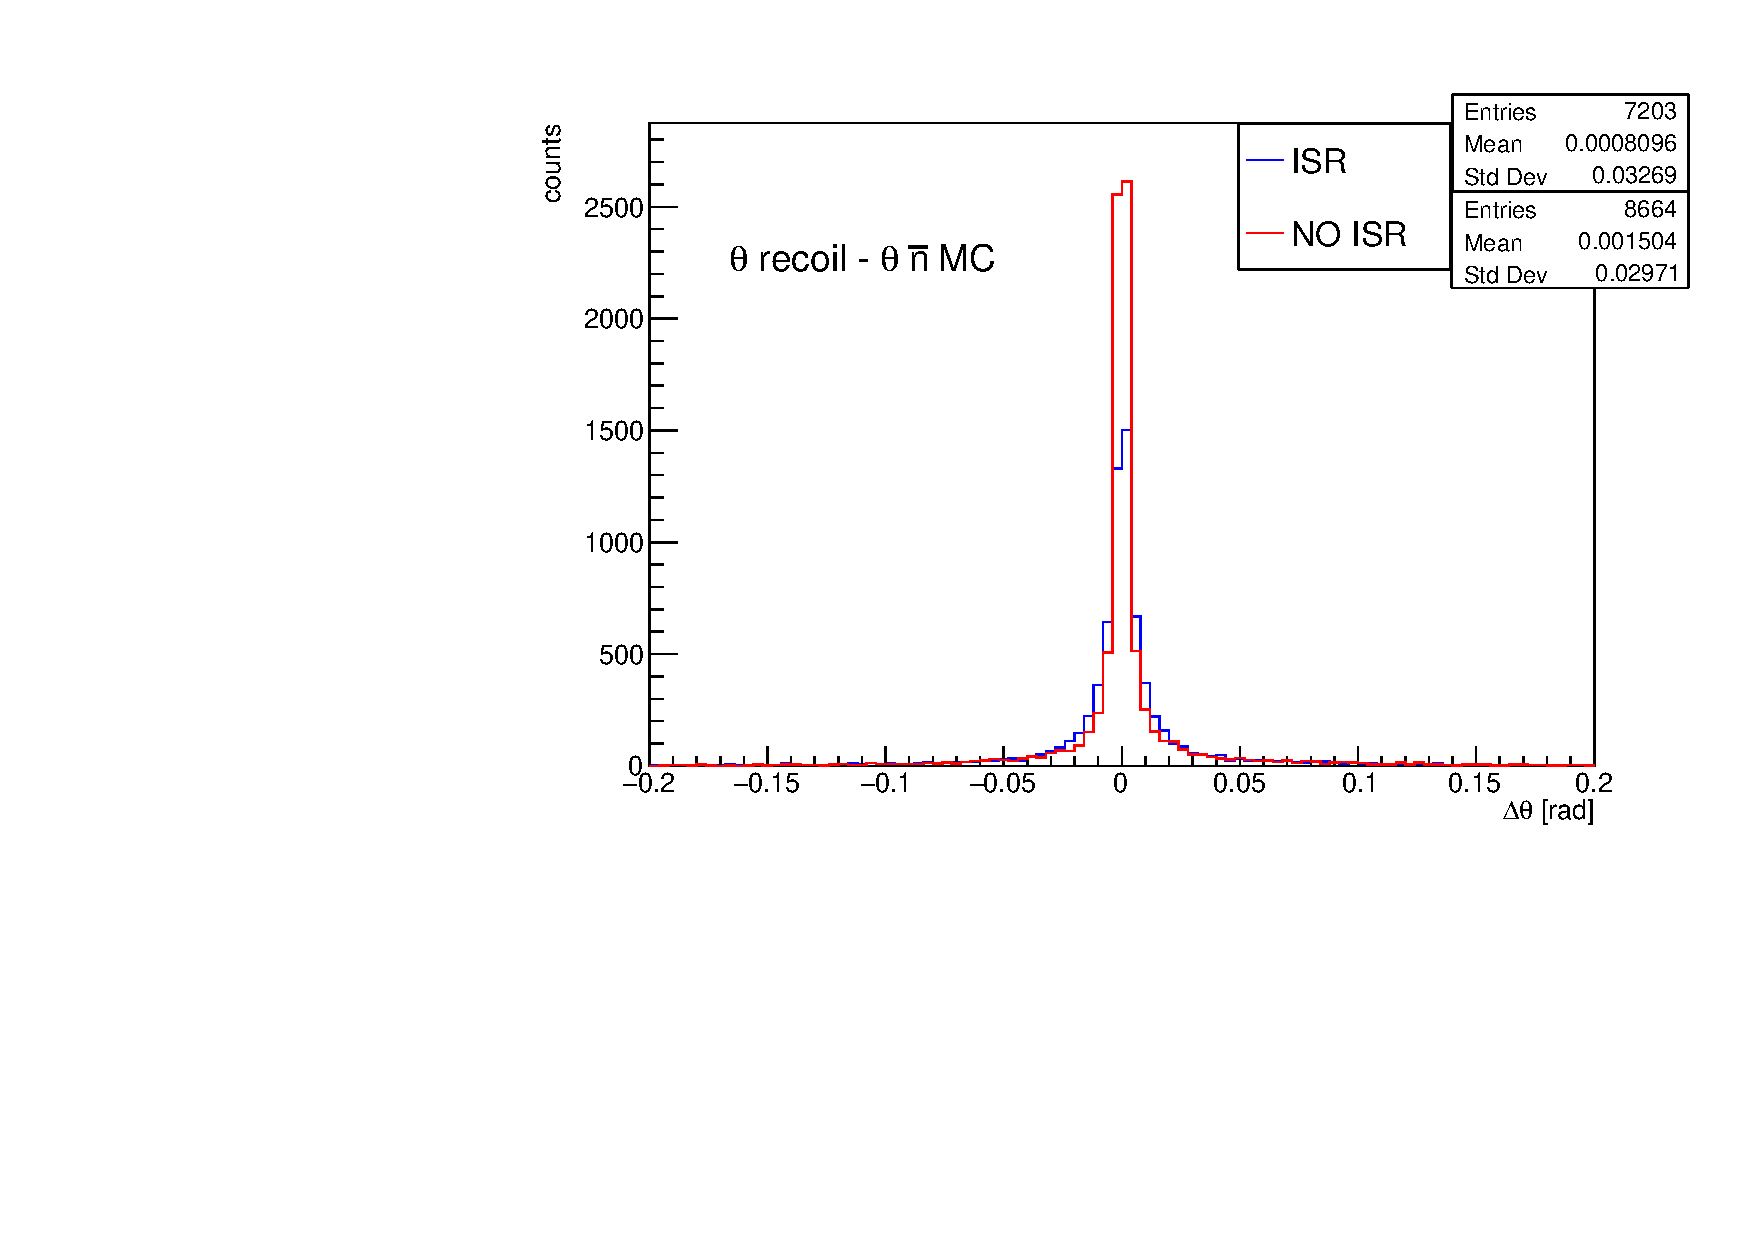
\includegraphics[width=0.49\textwidth]{nbar_MC/images/kin_delta_theta_mc.pdf}
     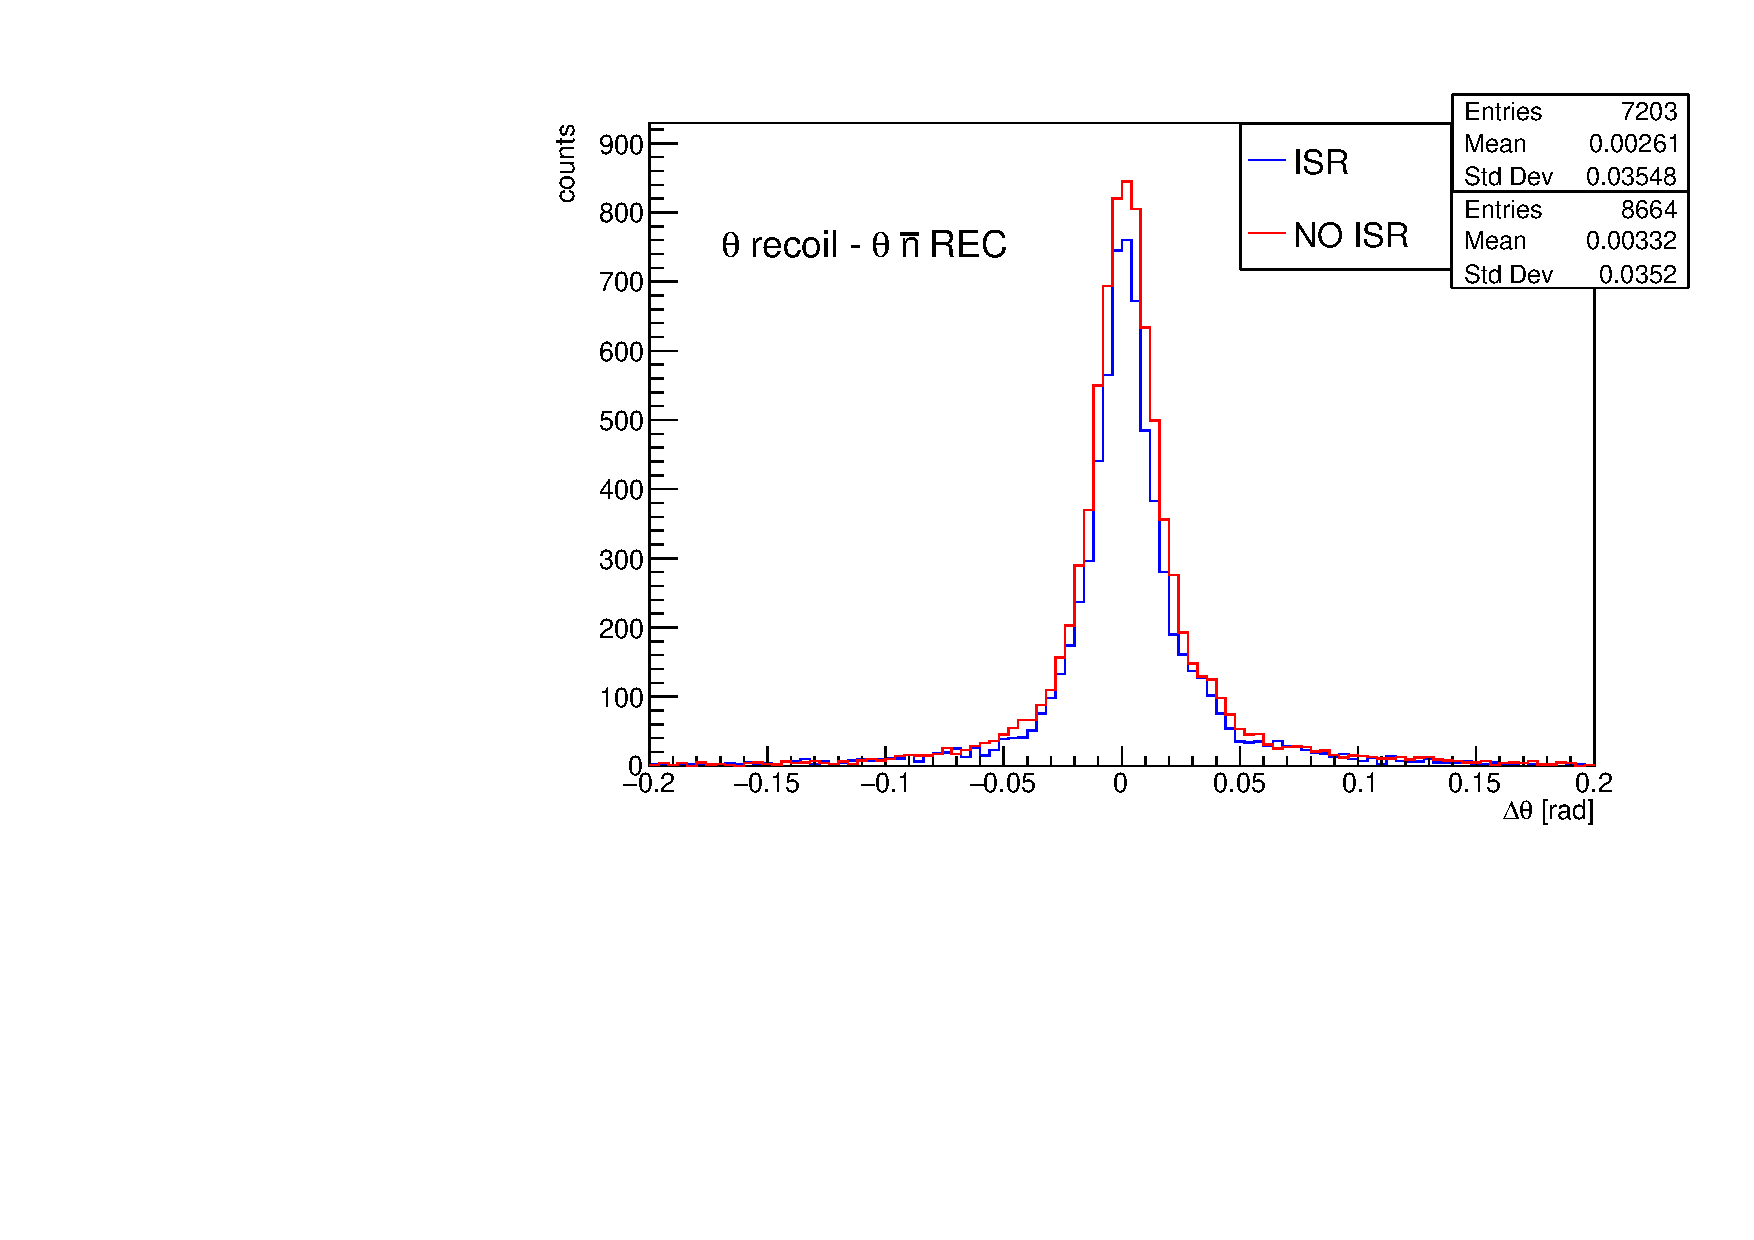
\includegraphics[width=0.49\textwidth]{nbar_MC/images/kin_delta_theta_rec.pdf}
     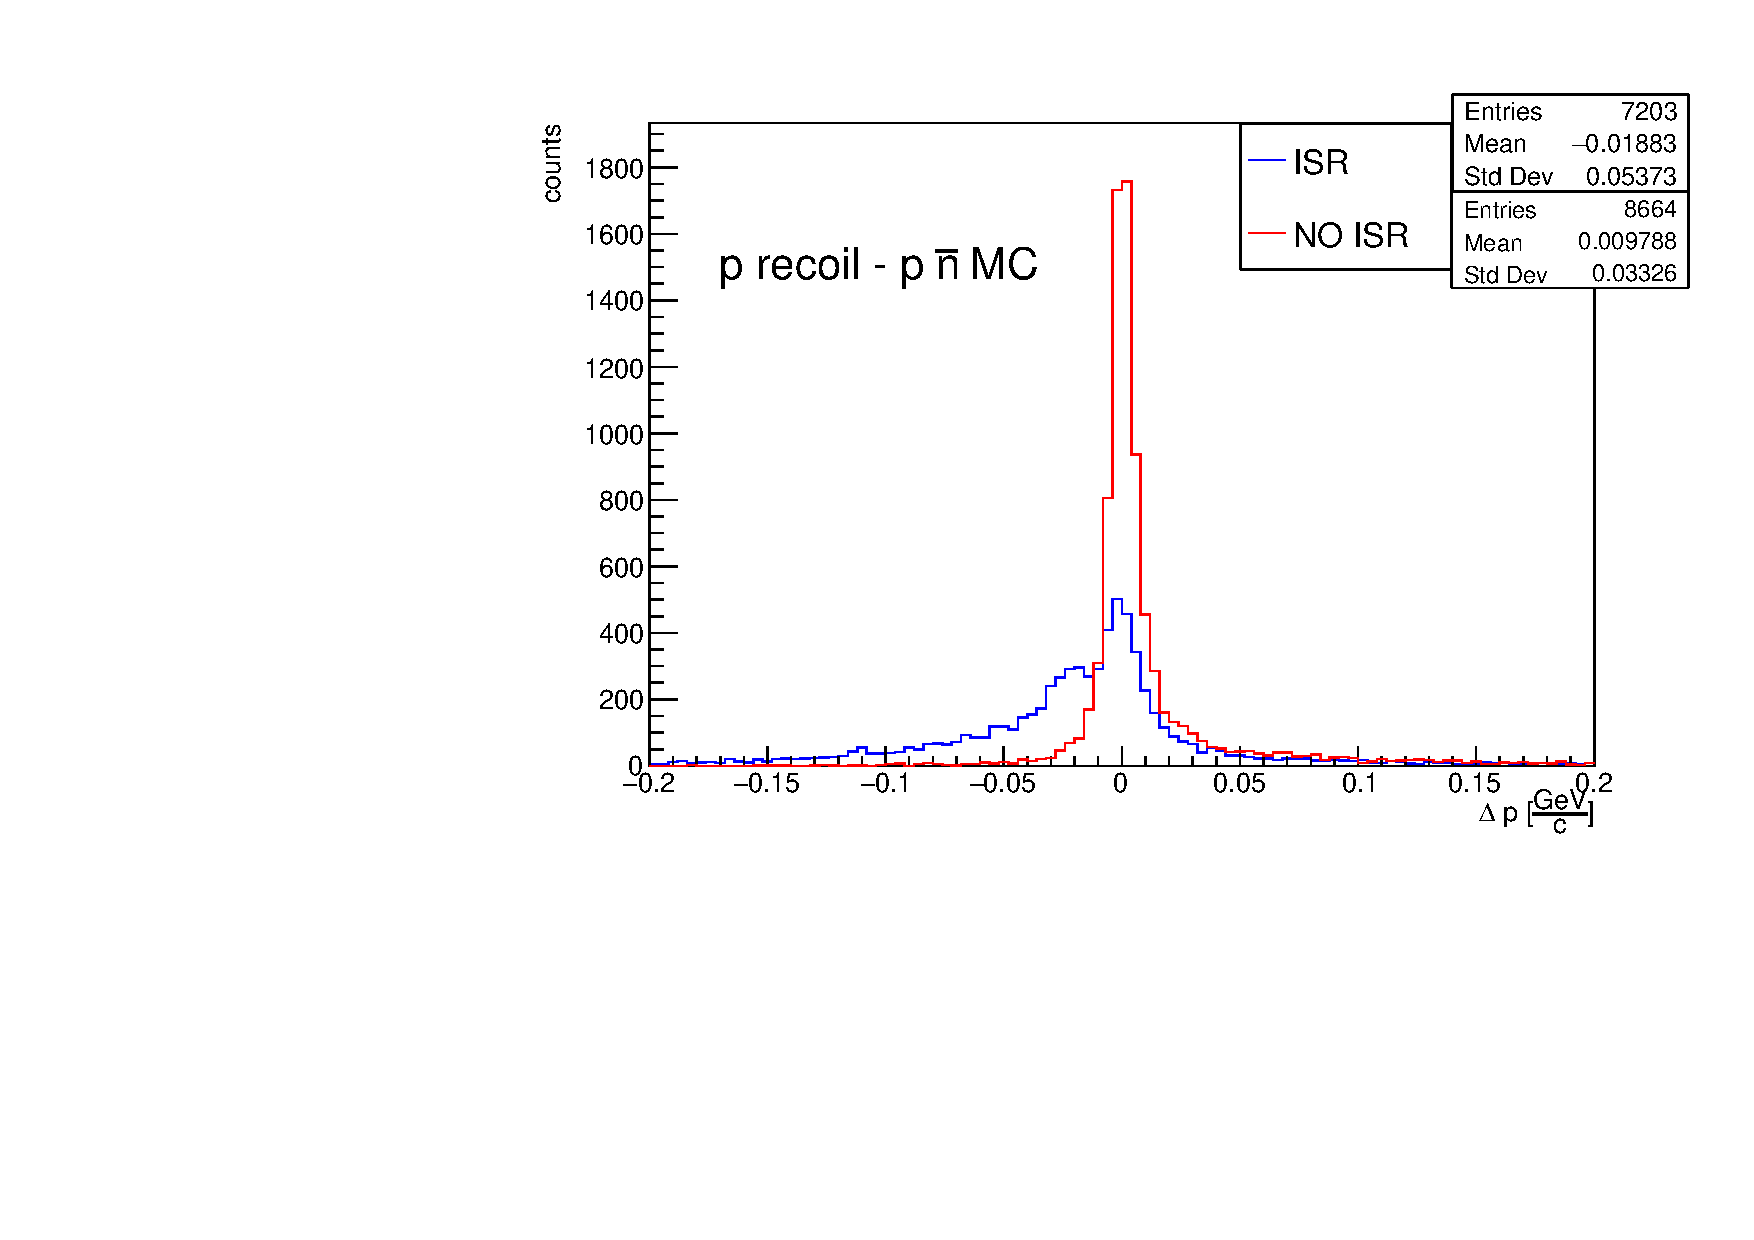
\includegraphics[width=0.49\textwidth]{nbar_MC/images/kin_delta_p_mc.pdf}
     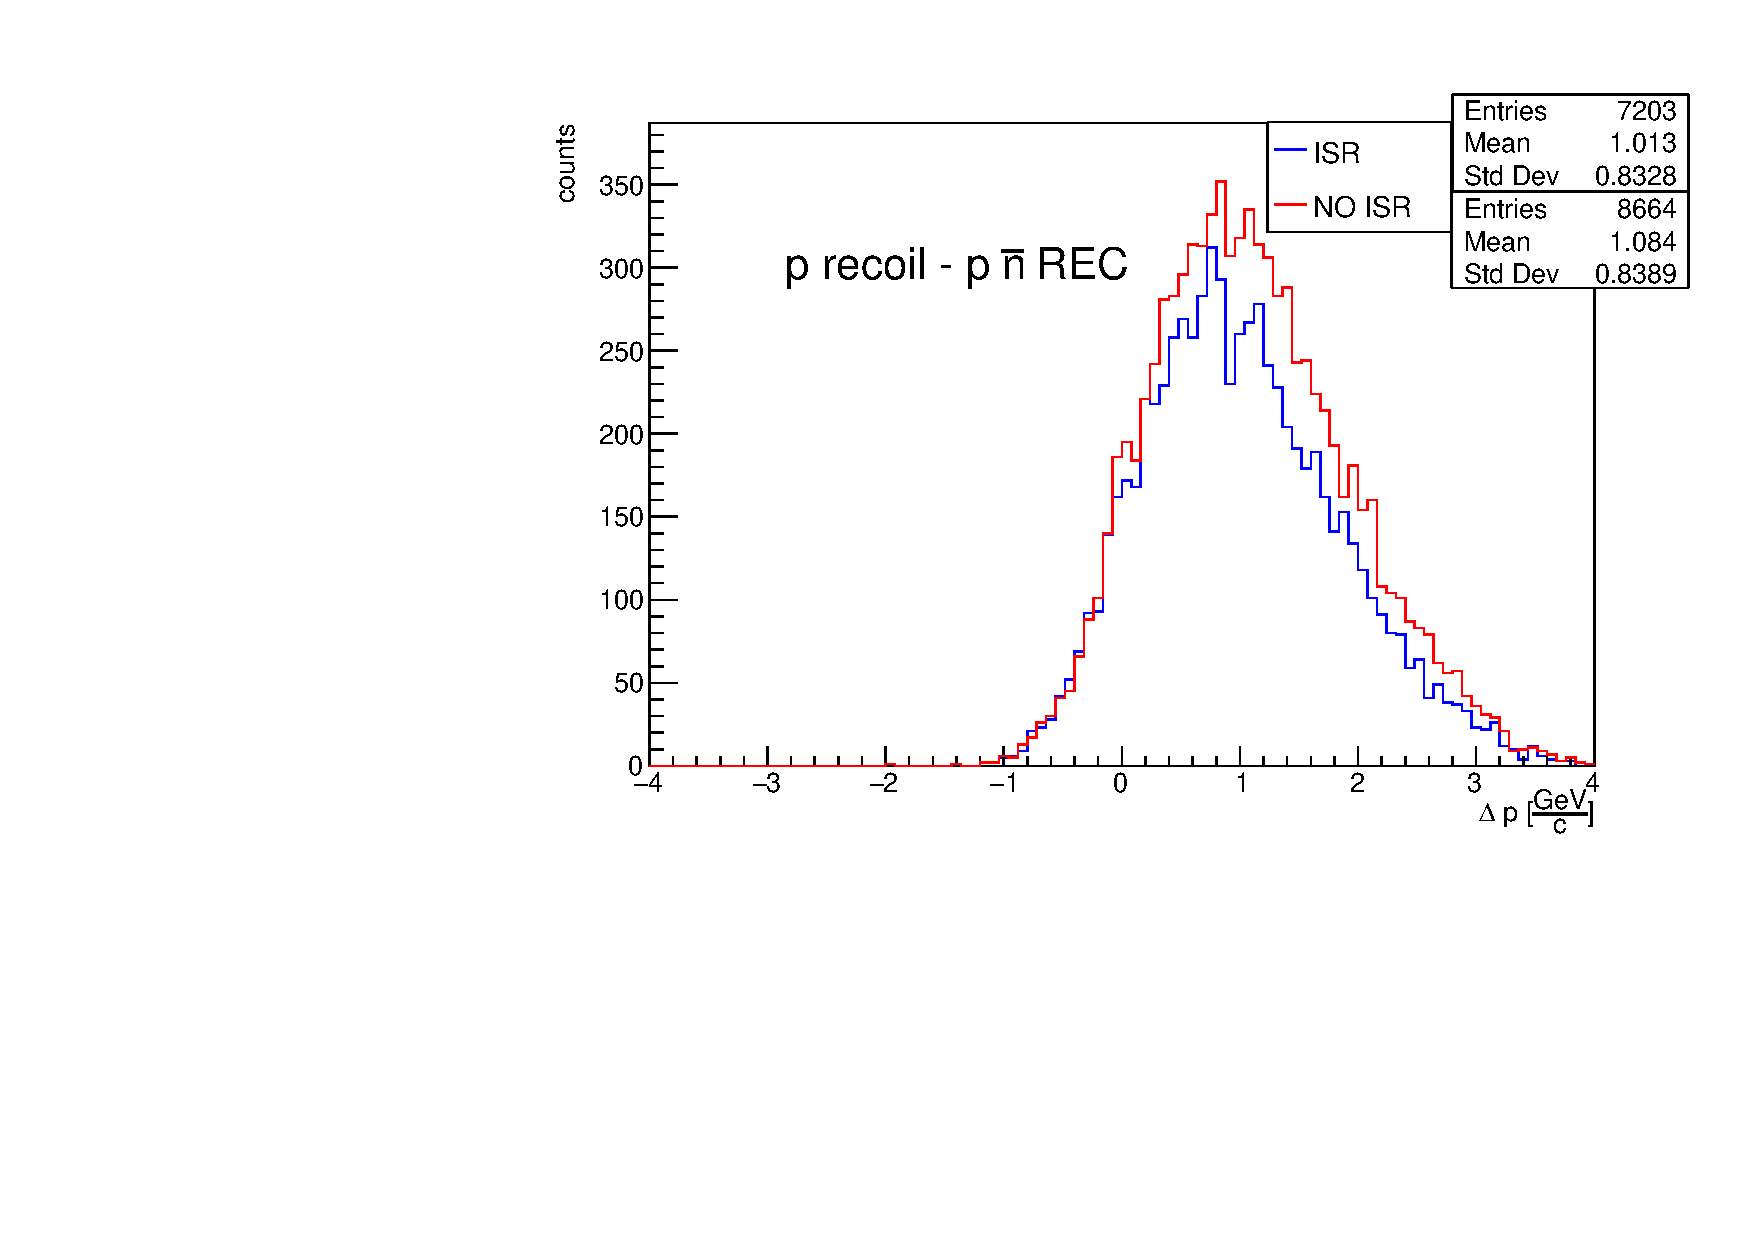
\includegraphics[width=0.49\textwidth]{nbar_MC/images/kin_delta_p_rec.pdf}
     \caption{Momentum and $\theta$ angle residuals distribution between recoil system and anti-neutron candidate, after the 1C Kinematic Fit procedure}
\end{figure}

As can be easily seen from the distributions, no significant improvement in recoil momentum resolution was observed post 1C Kinematic Fit compared to the unconstrained baseline ~\ref{fig:pRecoil-nP} . This confirms that the recoil system was already optimally reconstructed in the signal sample Monte Carlo. Further kinematic fit studies using a Monte Carlo cocktail are discussed in the next section.

\subsection{Shower shape variables in the signal sample}
The following chapter introduces the core of this thesis: the analysis of the \textbf{shower shape variables} of neutral ECL clusters associated with anti-neutron candidates. Since the final goal is to assess Data/MC agreement for these variables, the shower shape variables are first studied in an MC signal sample with no background channels present. The main idea is that particle identification can be achieved by studying the shower shapes and their characteristics.

\subsubsection{The analyzed shower shape variables}
The selected variables are the \textbf{cluster energy}, the \textbf{E1E9} variable, the \textbf{E9E21} variable, \textbf{Lateral Momentum}, \textbf{Second Moment}, \textbf{Zernike Moments} (50 and 41), and \textbf{Number of Hits}, which are described first. 

\paragraph{Cluster Energy}
$\\$
The Cluster Energy (\emph{clusterE} in the basf2 software), as the name suggests, represents the total energy deposited by the cluster associated with a given candidate particle, in this case the anti-neutron. It has units of GeV and only clusters with Cluster Energy above 20 MeV are stored by the reconstruction software.

\paragraph{Cluster E1E9 and E9E21}
In order to provide a proper definition of these variables (respectively \emph{clusterE1E9} and \emph{clusterE9E21} in the basf2 software), the following figure is shown below:

\begin{figure}[H]
    \centering
     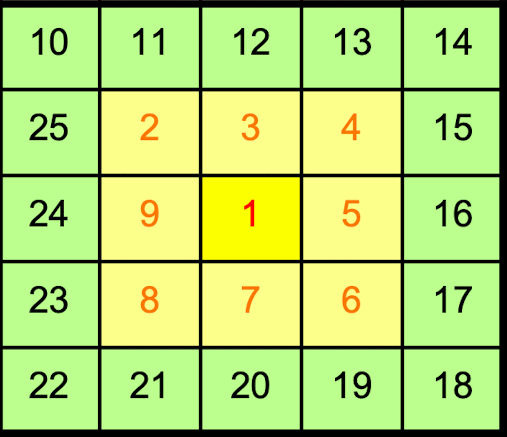
\includegraphics[width=0.50\textwidth]{nbar_MC/images/cluster}
     \caption{Ideal representation of a cluster pattern, consisting of a 5×5 matrix in which each cell corresponds to a single crystal}
\end{figure}

Cluster E1E9 and cluster E9E21 are defined as follow:

\begin{center}
$E1E9 = \frac{E_1}{\sum_{i=1}^{9} E_i}$ \hspace{0.2cm} $E9E21 = \frac{\sum_{j=1}^{9} E_j}{\sum_{j=10}^{25} E_j}$, with $j \ne 10,14,18,22$
\end{center}

The first one returns the ratio of the energy in the central crystal ($E_1$) to the total energy in the surrounding 3$\times$3 crystal grid ($E_9$). The second one returns the ratio of the energy in the 3x3 crystal grid around the central crystal ($E_1$) to the total energy in the 5$\times$5 crystal grid around the central crystal, excluding the corners. 
 $\\$
These ratios are always less than 1 and tend toward larger values for photons and smaller values for hadrons, as the latter produce more spread-out showers. These variables are dimensionless and are included within the range $[0,1]$.

\paragraph{Lateral Momentum}
$\\$
The cluster Lateral Momentum or Lateral Energy distribution (\emph{clusterLAT} in the basf2 software) is defined as follow:

\begin{center}
$C_{LM} = \frac{ \sum\limits_{i=2}^n E_i r_i^2} {  E_0 r_0^2 + E_1 r_0^2+ \sum\limits_{i=2}^n E_i r_i^2}$, 
\end{center}
with $r_0 \simeq 5$ cm (average distance between two crystals centres).  
$\\$
$n$ is the number of crystals associated to the shower, $E_i = (E_0,E_1,...)$  are the crystal energies sorted by descending energy and $r_i$ is the distance of the i-th digit to the shower center projected onto a plane perpendicular to the shower axis. For radially-symmetric electromagnetic showers, this variable peaks at $\sim 0.3$, where it is larger for hadronic particles. This variable is dimensionless and it is included within the range $[0,1]$.

\paragraph{Second Moment}
$\\$
The cluster Second Moment (\emph{clusterSecondMoment} in the basf2 software) is defined as follow:

\begin{center}
$C_{SM} = \frac{1}{S_0}\frac{ \sum\limits_{i=0}^n  E_i r_i^2} { \sum\limits_{i=0}^n E_i}$,
\end{center}
where $E_i$ and $r_i$ are the same variables as used for the lateral momentum, while $S_0$ is a normalization factor that normalizes to 1 for isolated photons, making $C_{SM}$ dimensionless. The Second Moment measures the dispersion of cluster size.

\paragraph{Zernike Moments}
$\\$
The Zernike Moments (Zernike Polynomials) are a set of orthogonal functions which are defined on the unit disk. Since each moment represents a specific pattern shape, they are widely used to represent smooth, two‑dimensional functions (especially wavefronts) over circular apertures. 
$\\$
On the unit disk parametrized by polar coordinates $(\rho,\phi)$ with $0 \le \rho \le 1$, the Zernike modes are usually written as:

   \begin{center}
	    $Z^{m}_n(\rho,\phi) = R^m_n(\rho)\,\cos(m\,\phi)$
	    
	    \vspace{0.3cm}
	    
	    $Z^{-m}_n(\rho,\phi) = R^m_n(\rho)\,\sin(m\,\phi)$	
     \end{center}  
    
Where:   
\begin{center}
 	$R^m_n(\rho) = \sum_{k=0}^{\tfrac{n-m}{2}} \frac{(-1)^k\,(n-k)!}{k!\left (\tfrac{n+m}{2}-k \right )! \left (\tfrac{n-m}{2}-k \right)!} \;\rho^{n-2\,k}$
 \end{center} 
 
$n$ represents the radial degree and $m$ represents the azimuthal frequency ($m = 0$ for spherical Zernike polynomials). A figure of the Zernike polynomials is given below:
\begin{figure}[H]
    \centering
     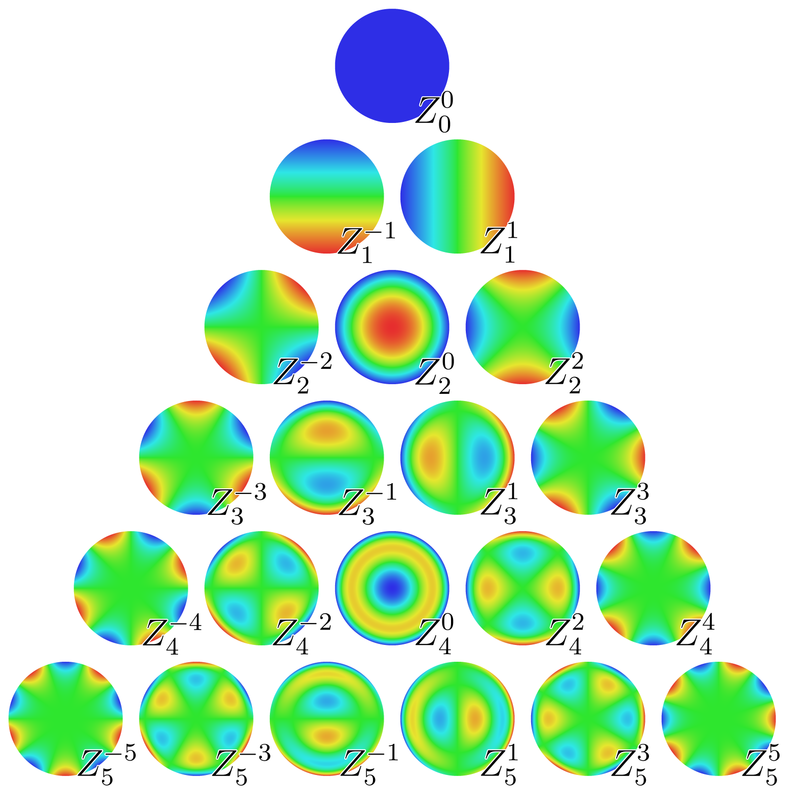
\includegraphics[width=0.60\textwidth]{nbar_MC/images/zernike}
     \caption{Zernike Polynomials representation. Moments $Z^0_4$ and $Z^1_5$ are widely discussed in this thesis}
\end{figure}

Precisely, Zernike Moments  $Z^0_4$ and $Z^1_5$ (\emph{clusterAbsZernikeMomen40} and \emph{clusterAbsZernikeMoment51} in the basf2 software) are studied in this thesis, where the first one represents the radial spread distribution structure, while the second one represents the level of dipolar asymmetry.

\paragraph{Number of Crystals hit}
$\\$
The variable Number of Crystals hit (\emph{clusterNhits} in the basf2 software) returns sum of weights $w_i$, with $w_i \le 1$ of all crystals in the cluster. For non-overlapping clusters this is equal to the number of crystals in the cluster. However, in the case of overlapping clusters where individual crystal energies are split among them, this can be a non-integer value.

\subsubsection{Anti-neutrons ECL cluster variables}
In order to isolate the contribution of the neutral clusters which are correctly associated with $\bar{n}$ particles (Monte Carlo PDG = -2112) ({\color{red} red distribution}) from all $\bar{n}$ candidates ({\color{blue} blue distribution}), the two distributions are overlaid for each cluster variable. The former is naturally included within the latter, naturally.
\newpage
The obtained cluster variables in ISR case are shown below:
 \begin{figure}[H]
    \centering
    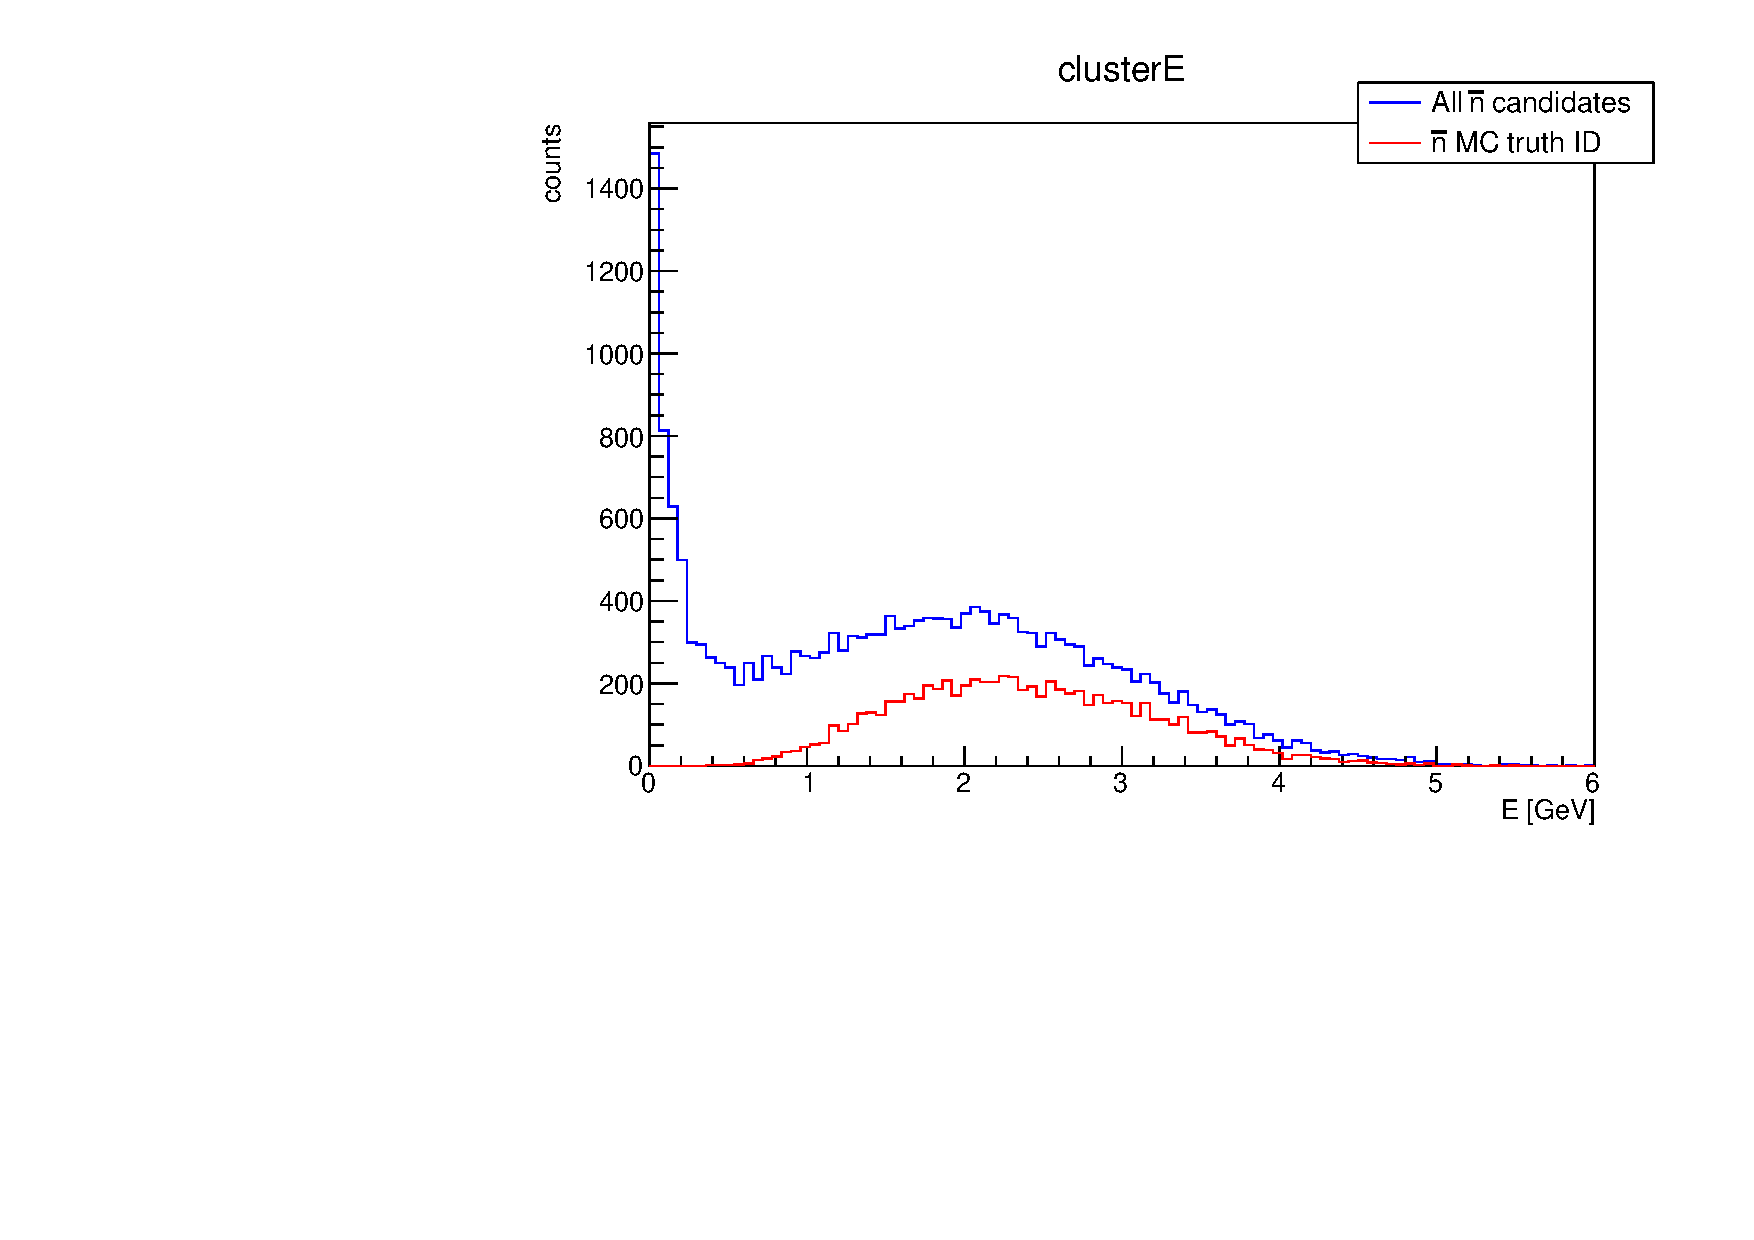
\includegraphics[width=0.49\textwidth]{nbar_MC/images/clusterE_isr.pdf}
    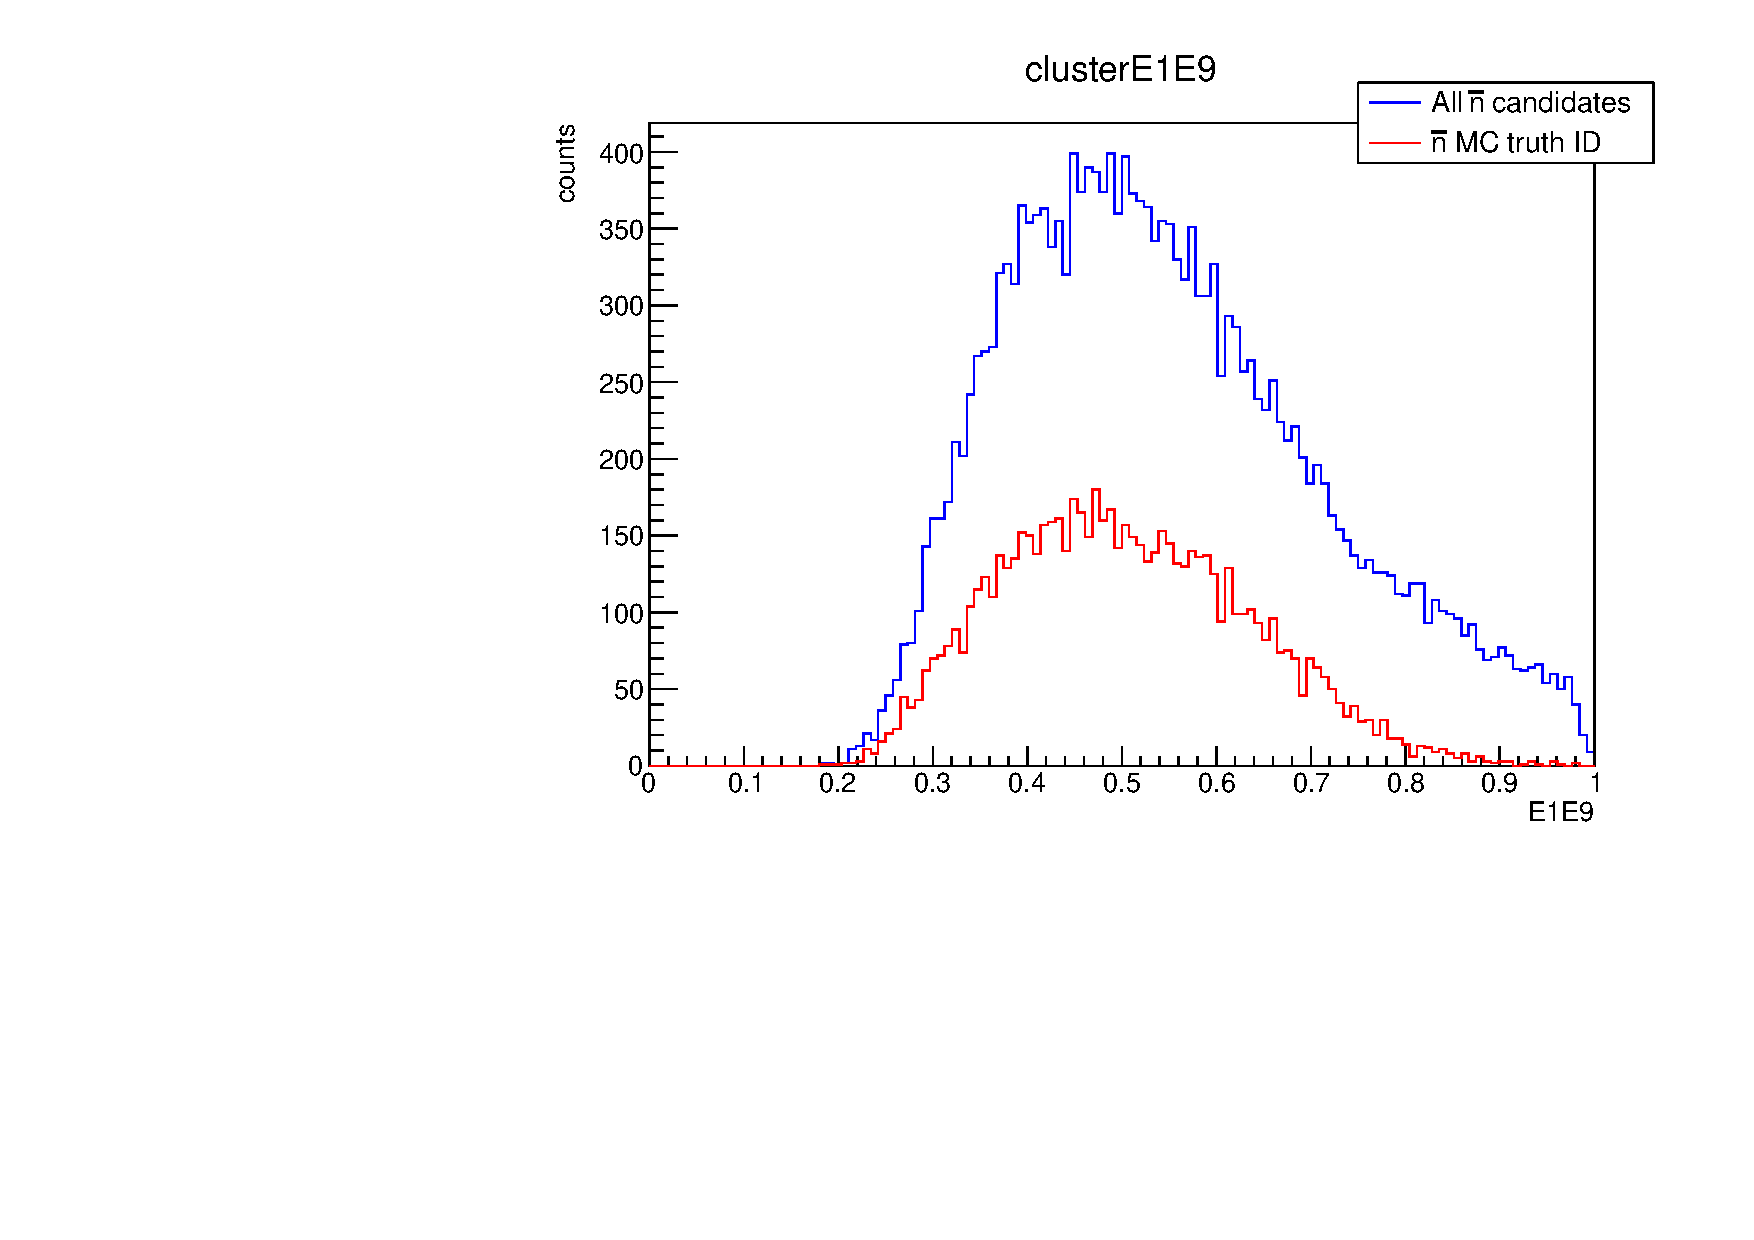
\includegraphics[width=0.49\textwidth]{nbar_MC/images/clusterE1E9_isr.pdf}
    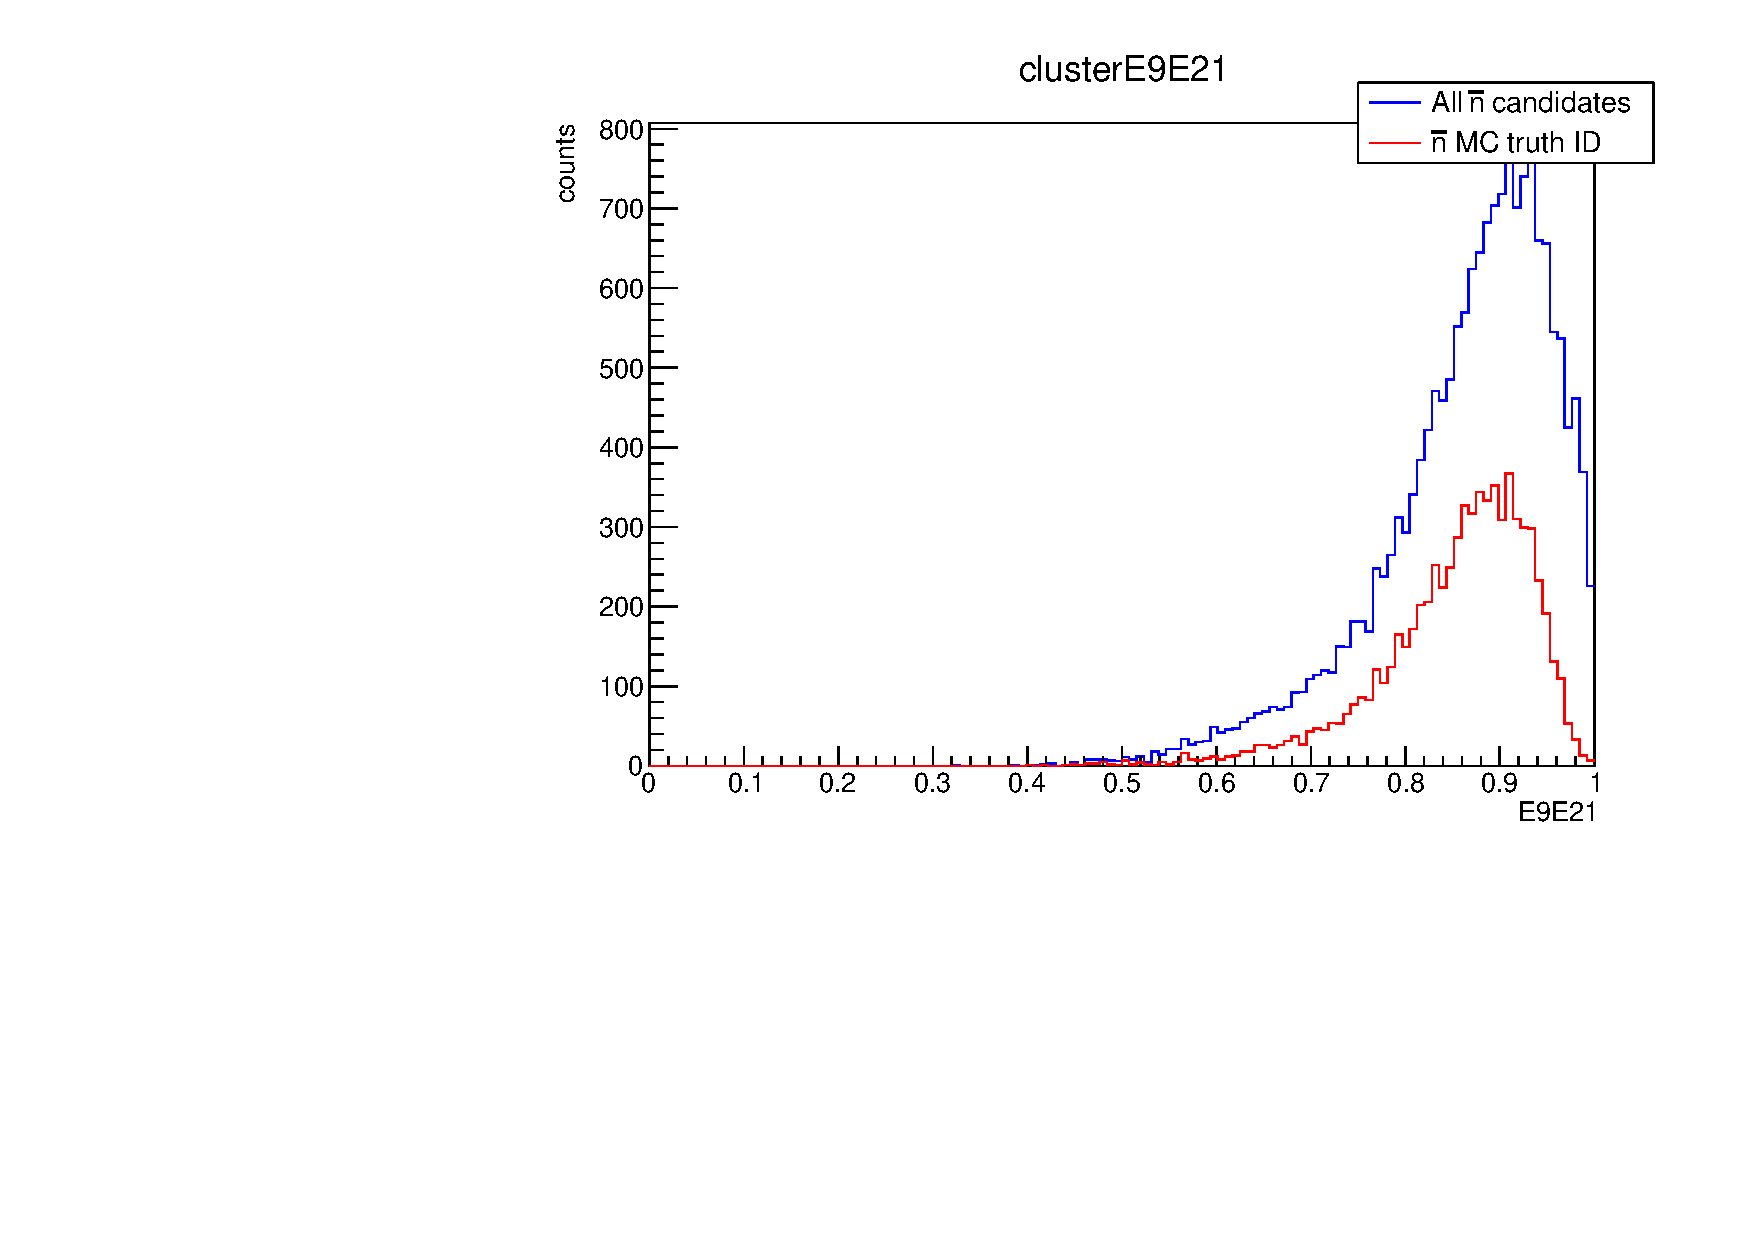
\includegraphics[width=0.49\textwidth]{nbar_MC/images/clusterE9E21_isr.pdf}
    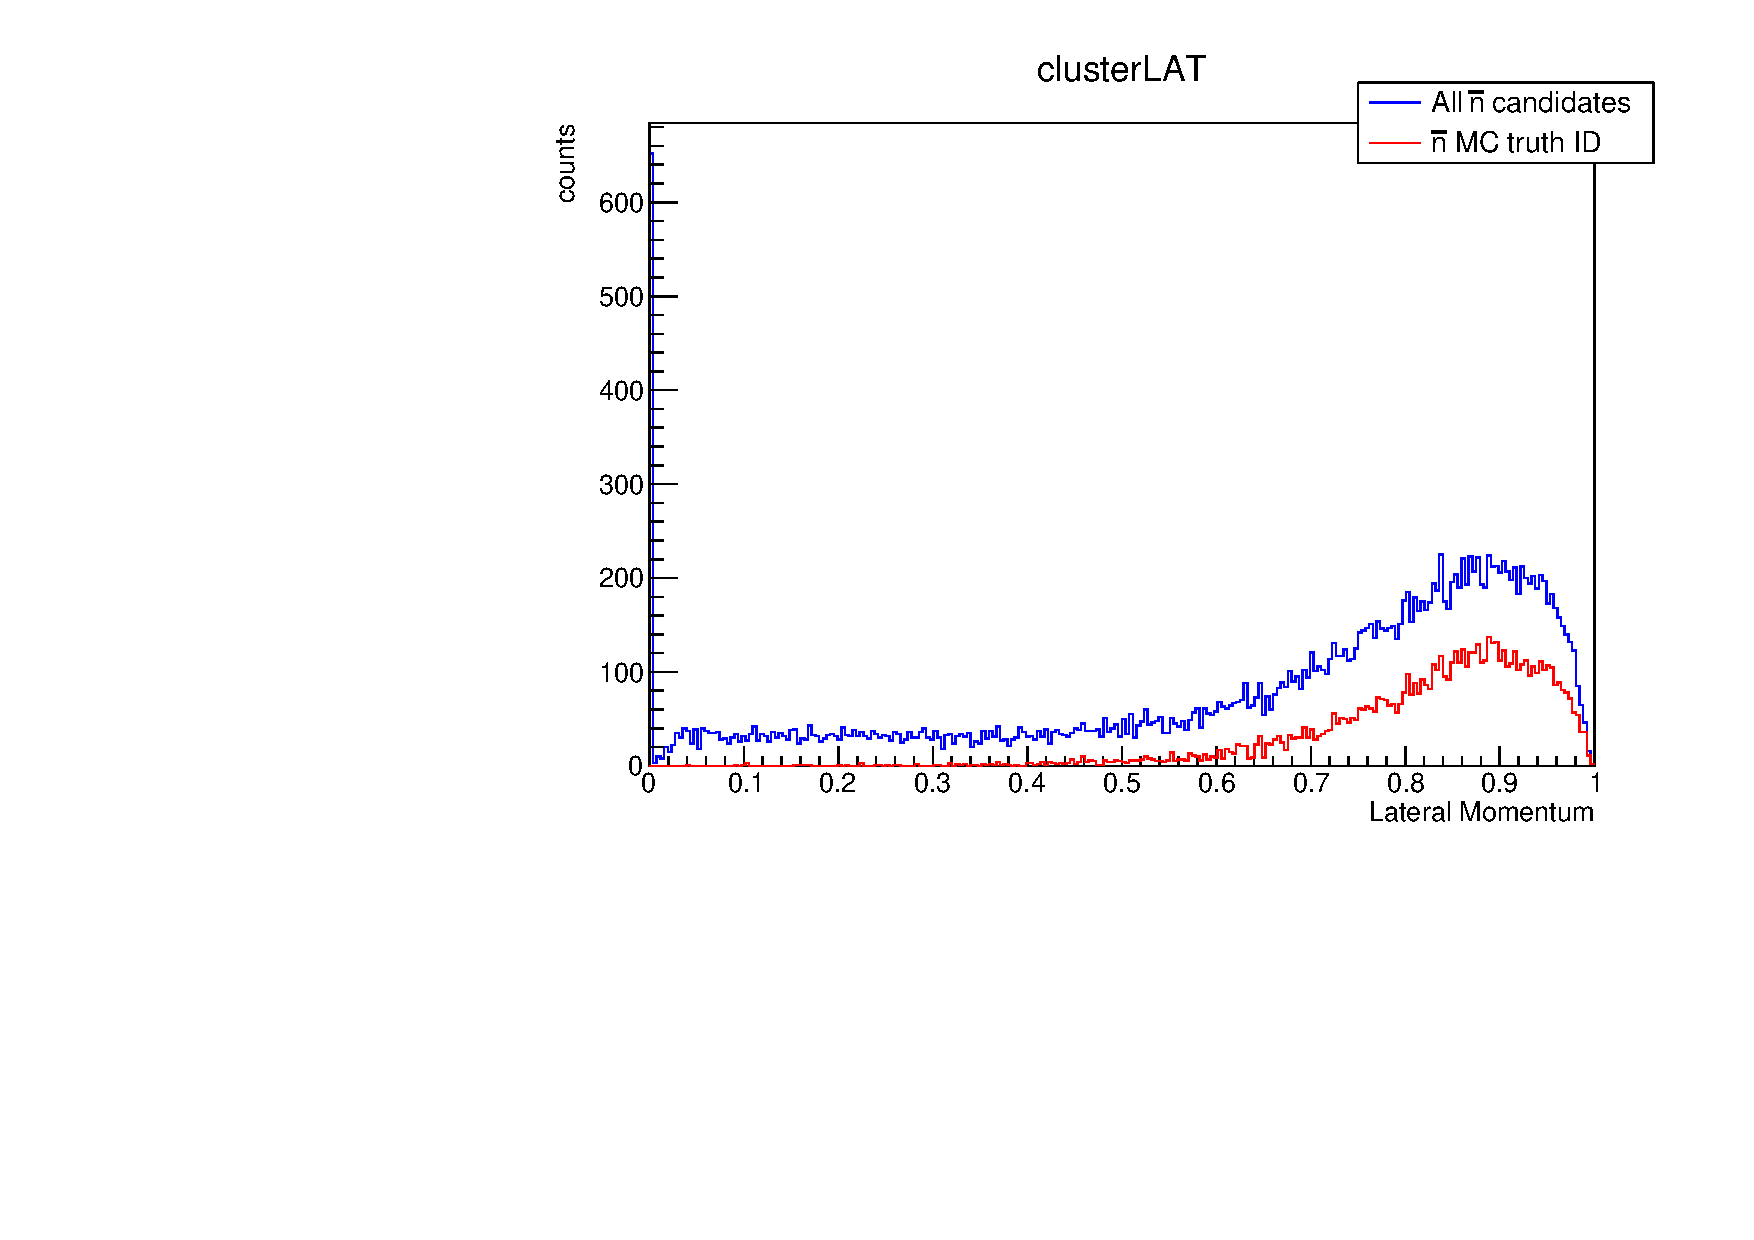
\includegraphics[width=0.49\textwidth]{nbar_MC/images/clusterLAT_isr.pdf}
    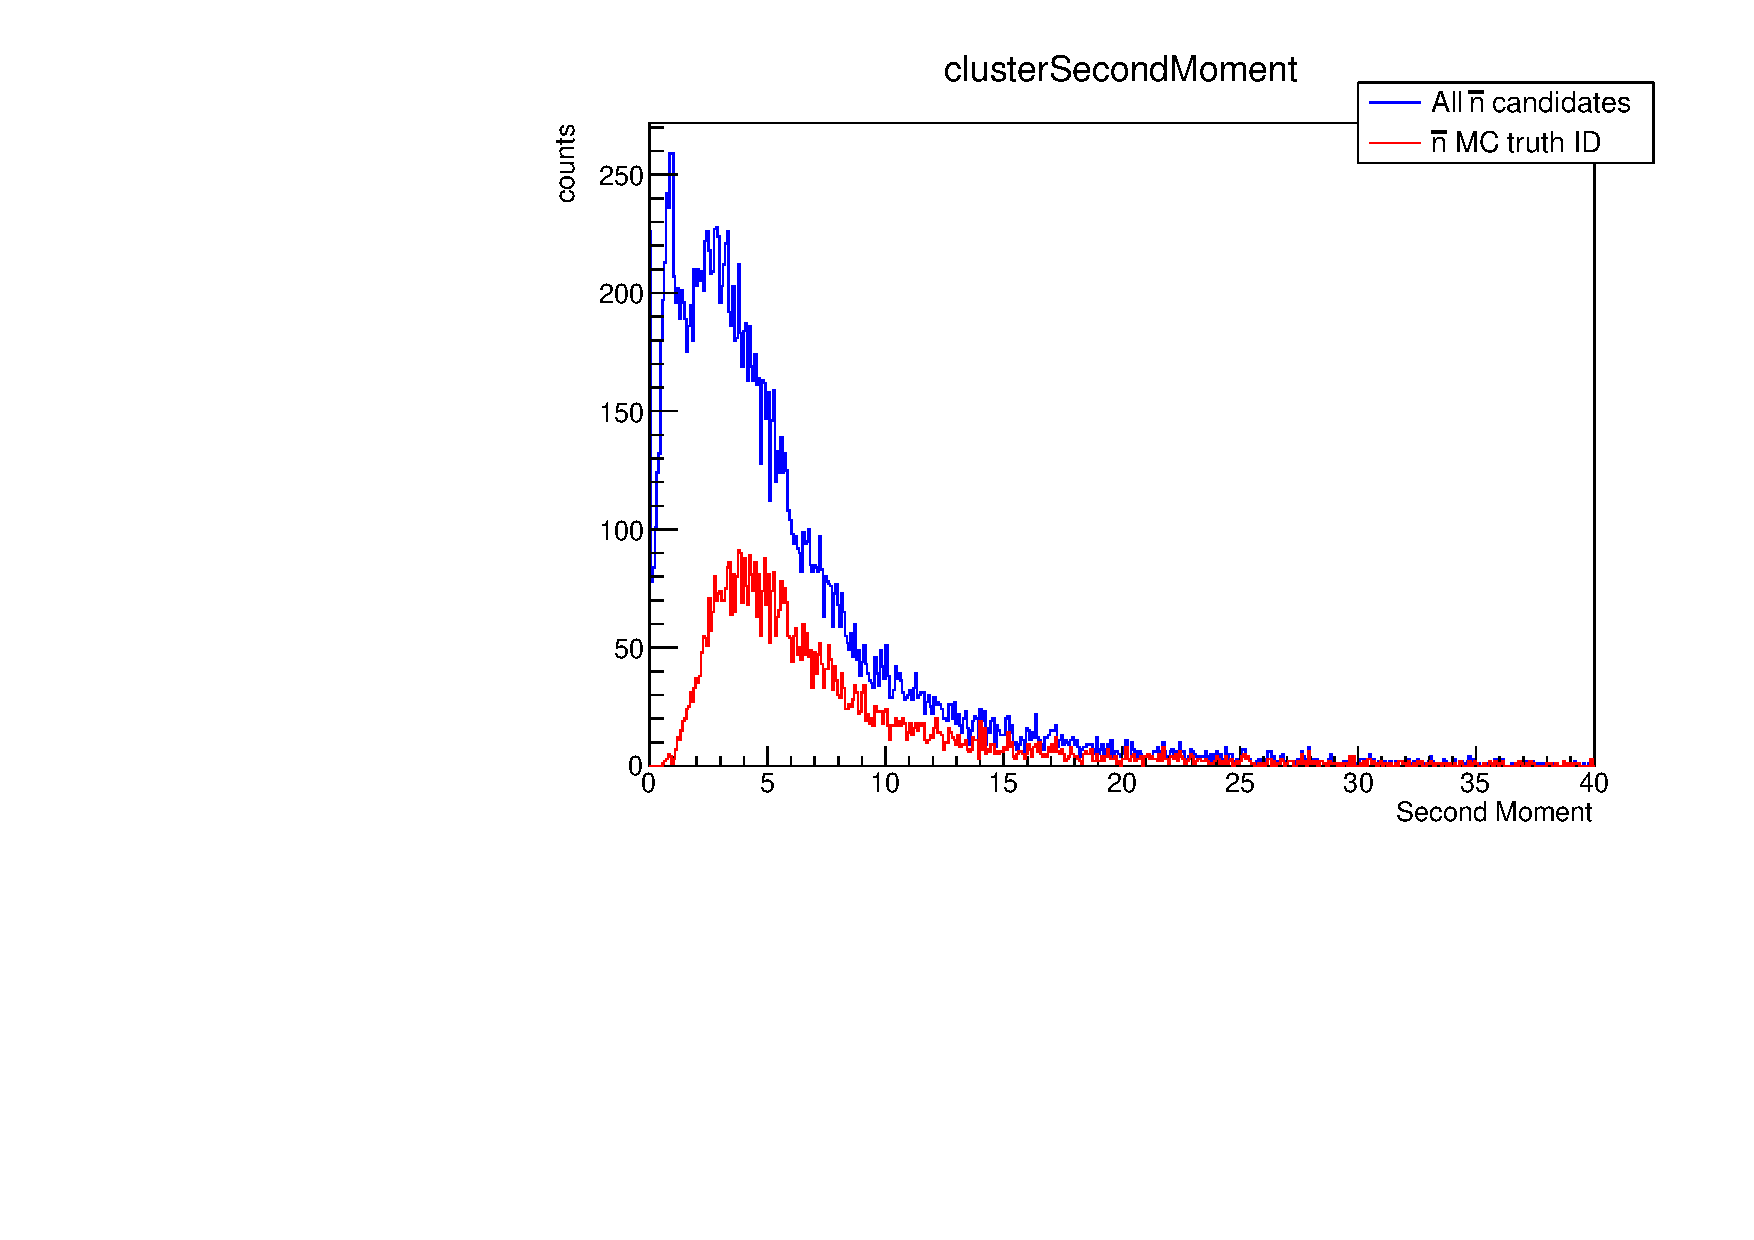
\includegraphics[width=0.49\textwidth]{nbar_MC/images/clusterSecondMoment_isr.pdf}
    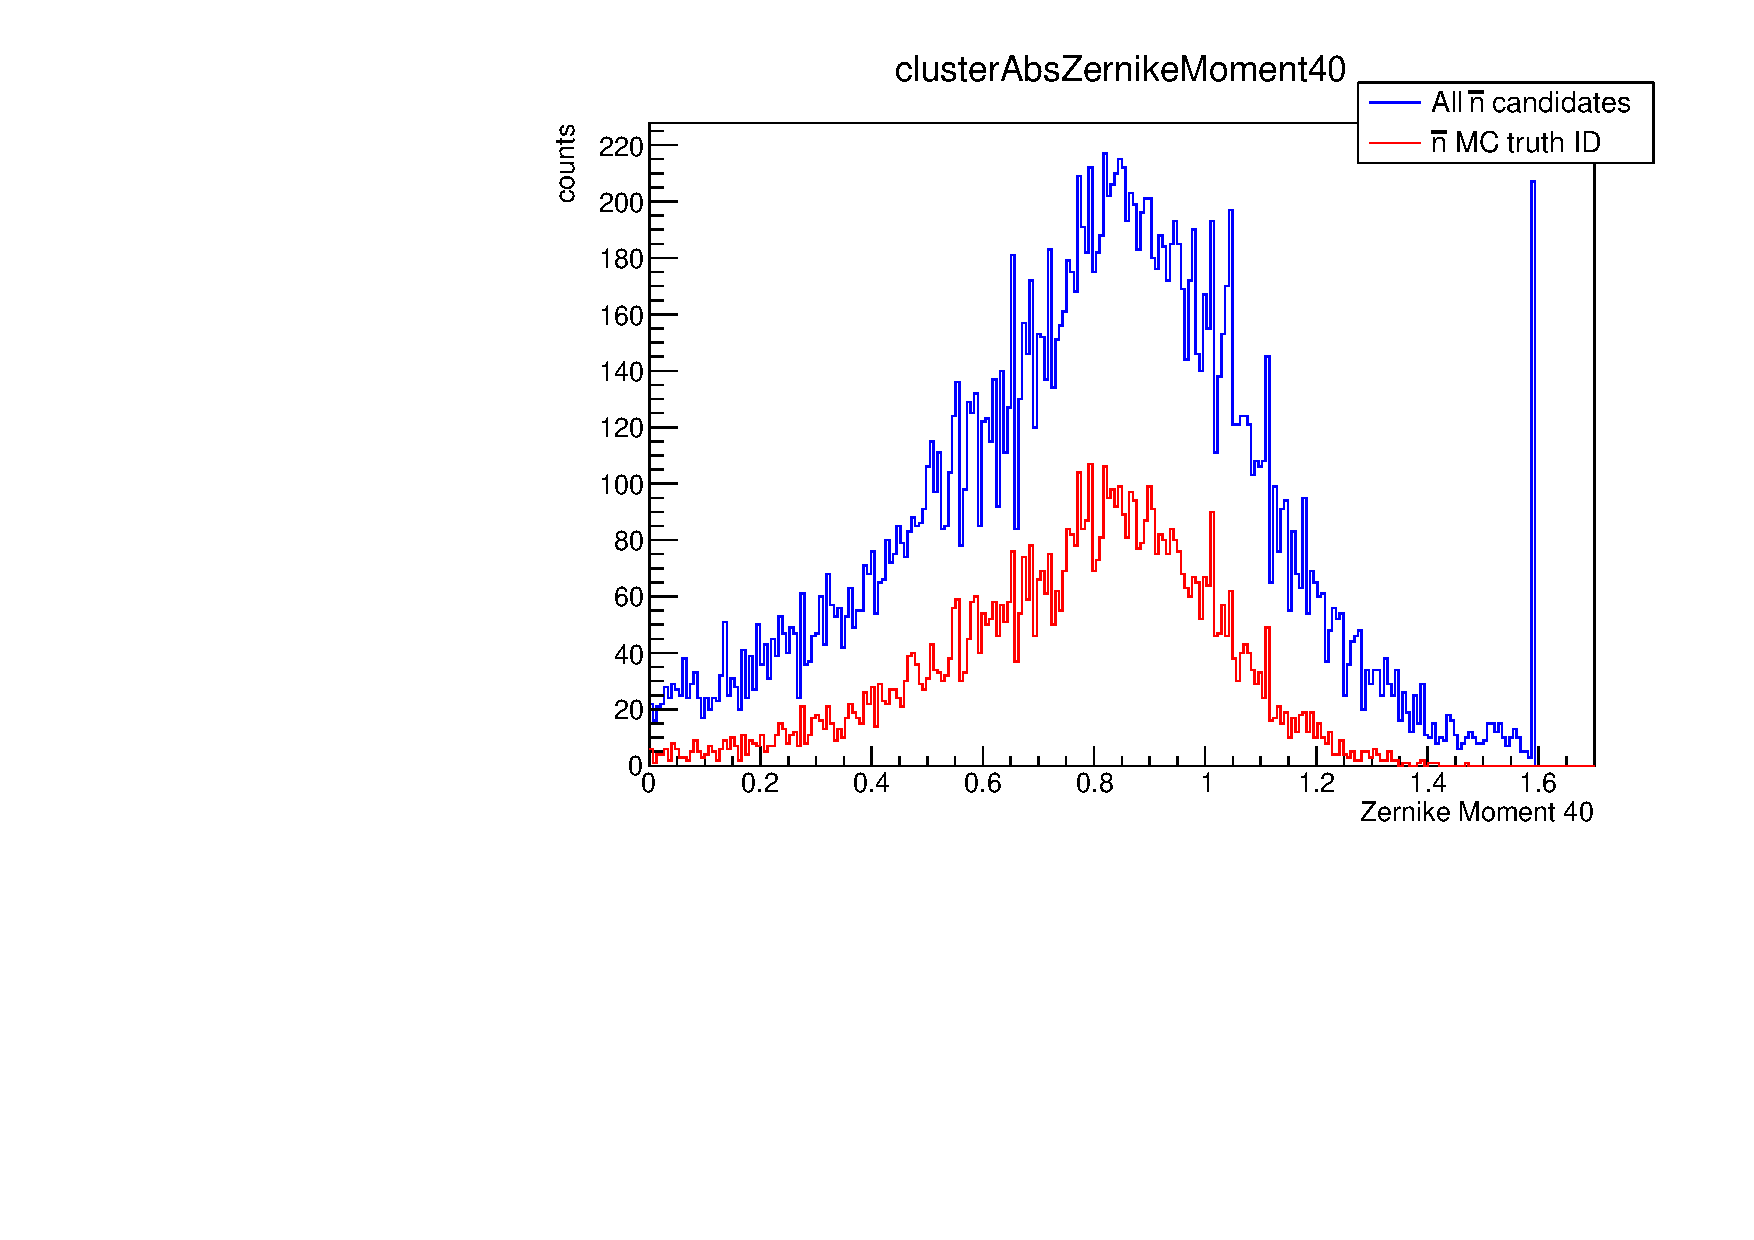
\includegraphics[width=0.49\textwidth]{nbar_MC/images/clusterAbsZernikeMoment40_isr.pdf}
    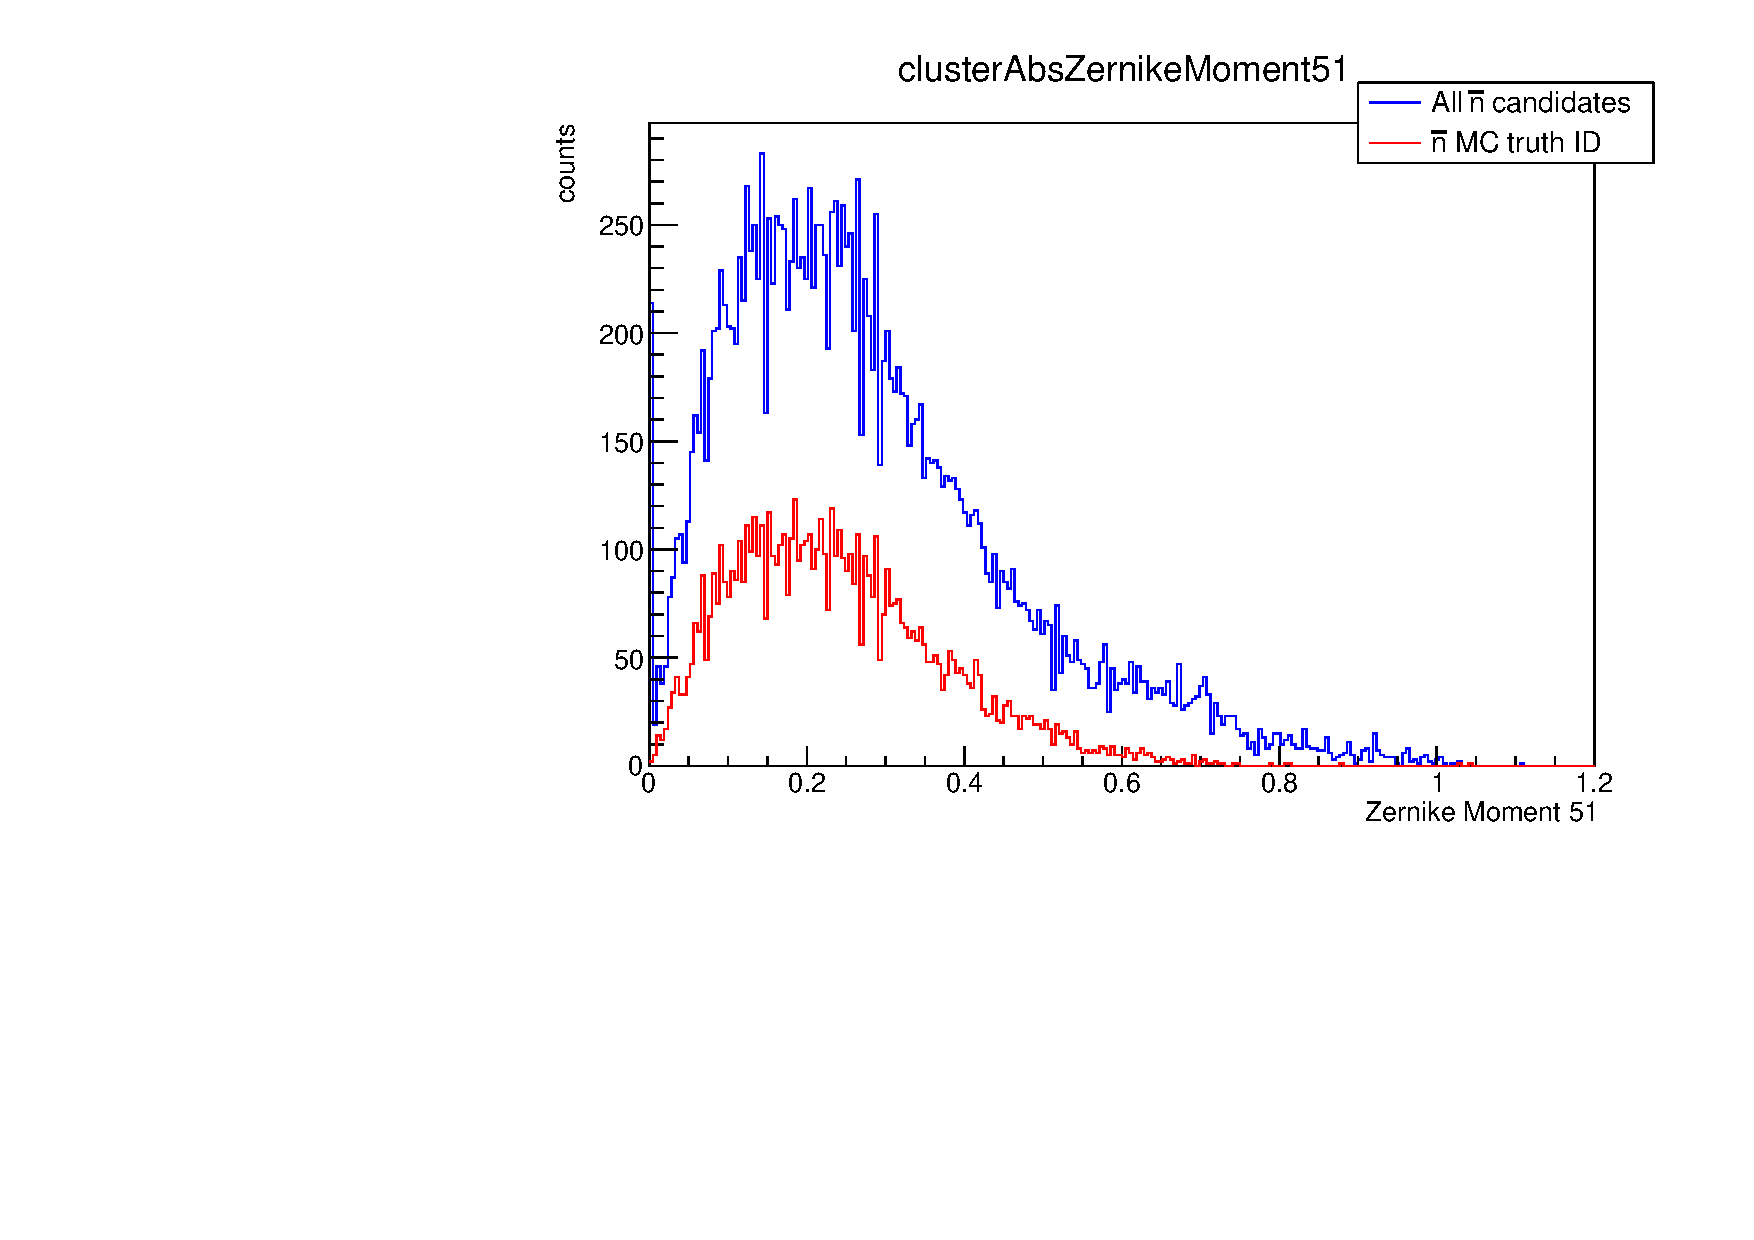
\includegraphics[width=0.49\textwidth]{nbar_MC/images/clusterAbsZernikeMoment51_isr.pdf}
    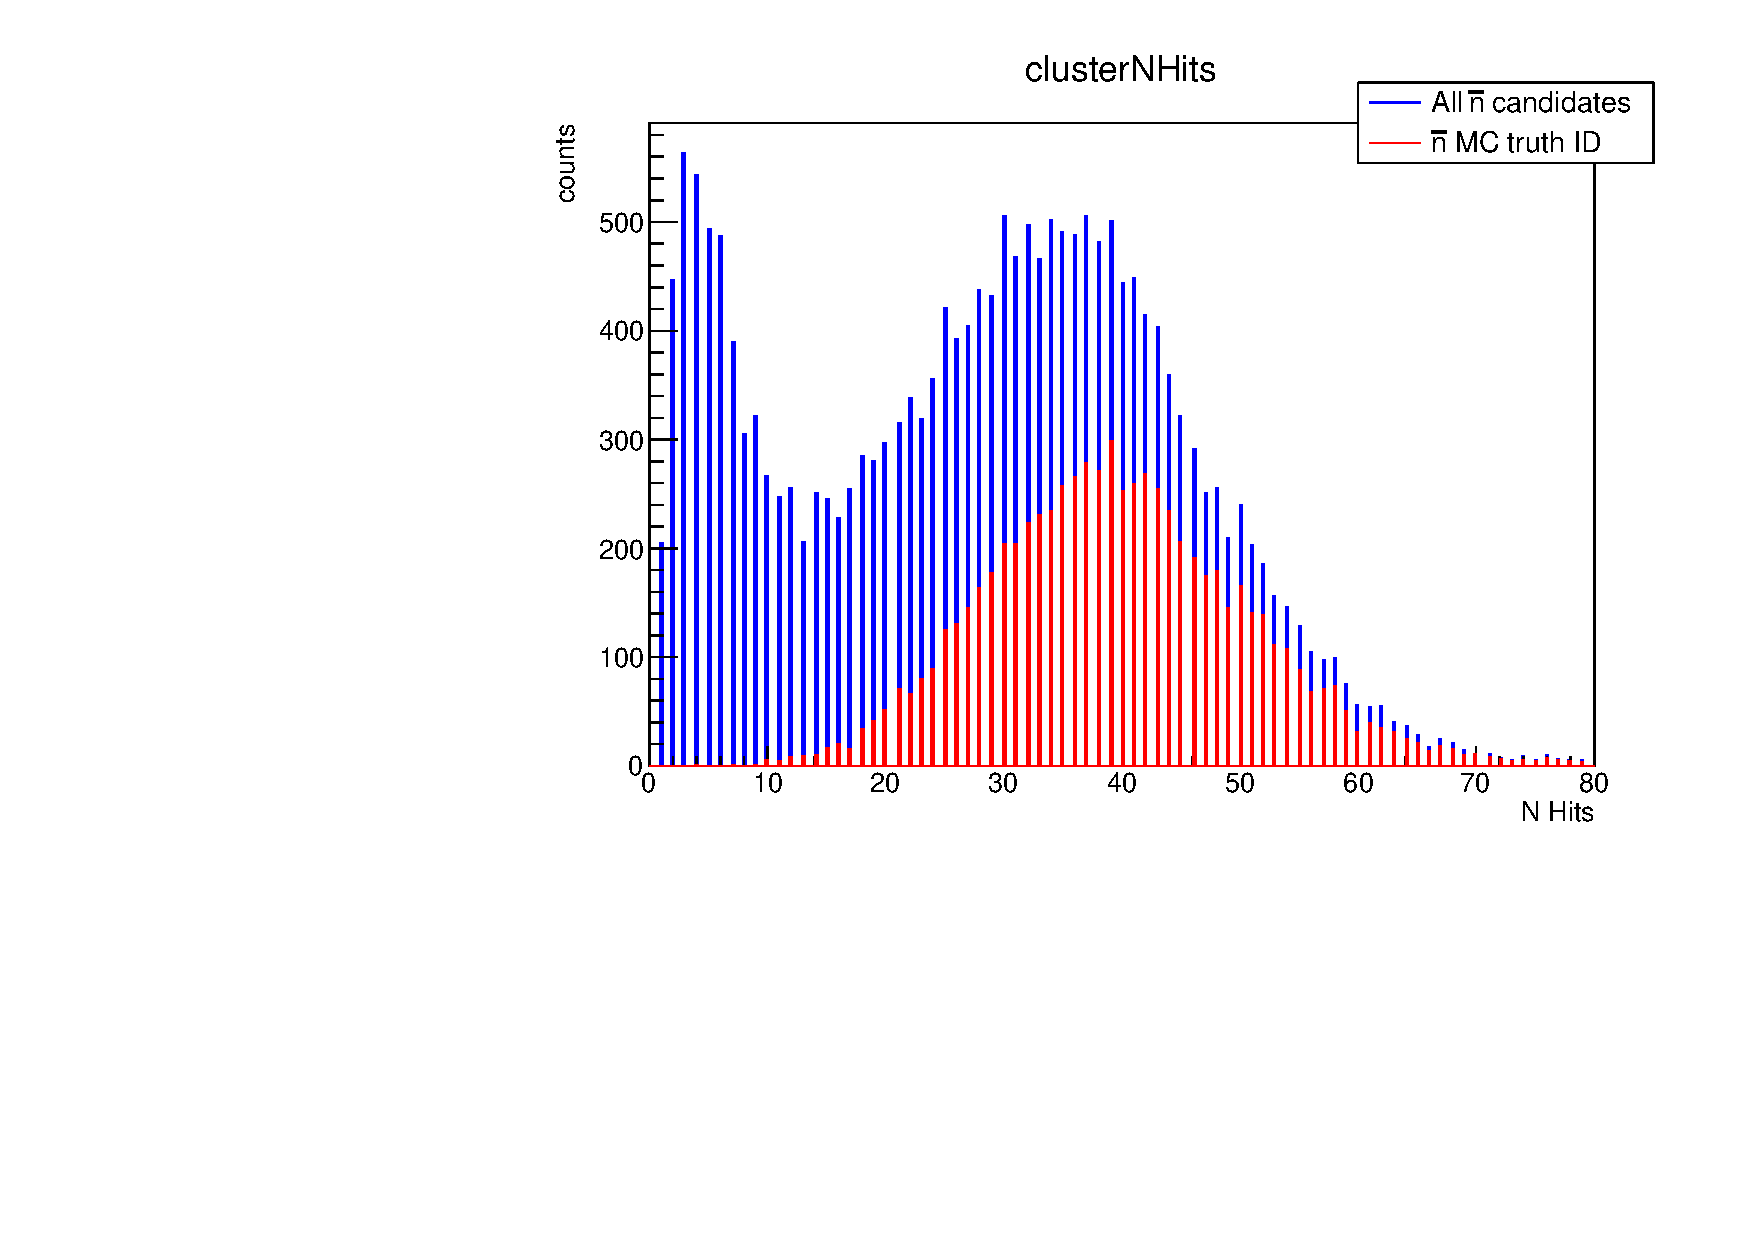
\includegraphics[width=0.49\textwidth]{nbar_MC/images/clusterNHits_isr.pdf}
   
     \caption{Comparison of reconstructed cluster variables for all $\bar{n}$ candidates versus those associated with $\bar{n}$ particles by Monte Carlo truth Monte Carlo PDG = -2112 (ISR case). The selection is performed using the Monte Carlo PDG code ($-2112$), as previously discussed}

\end{figure}

\newpage
The obtained cluster variables in NO ISR case are shown below:
 \begin{figure}[H]
    \centering
    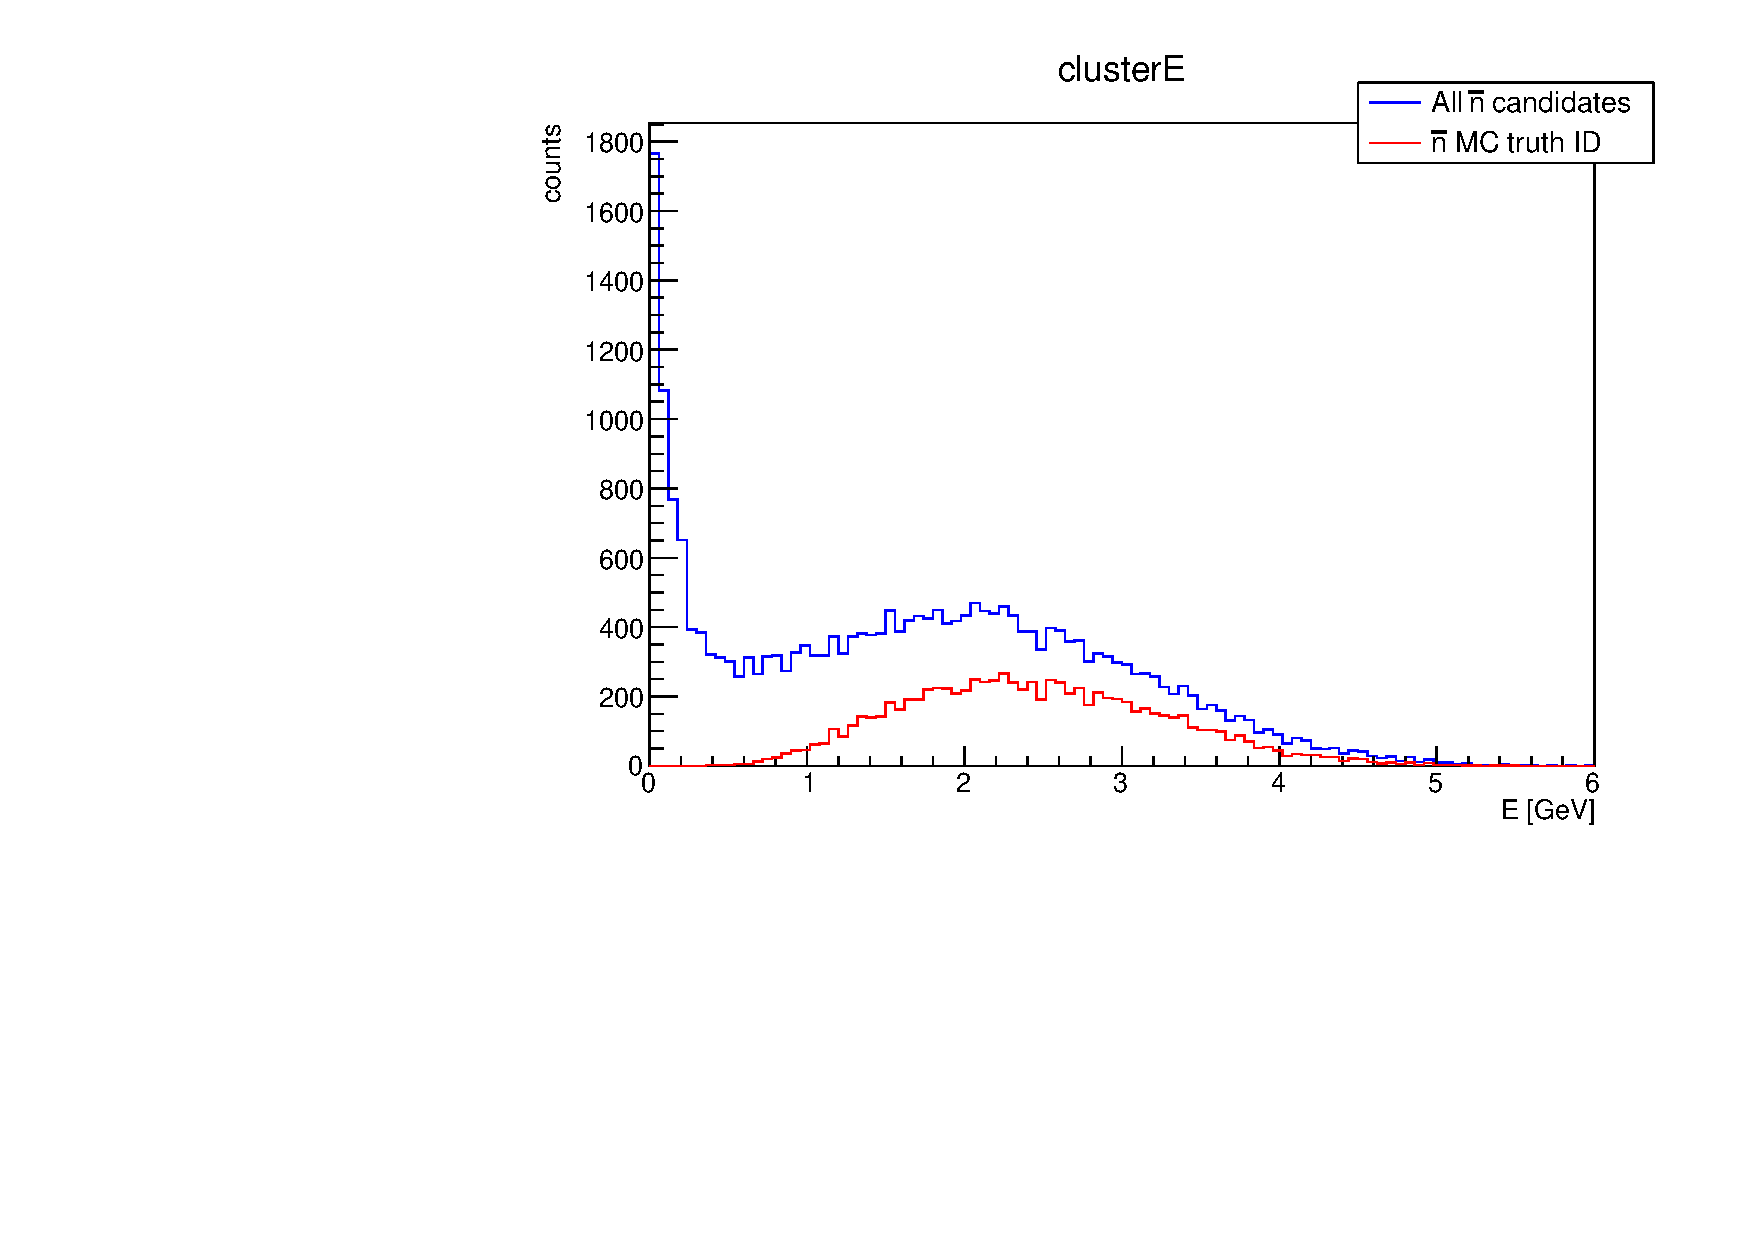
\includegraphics[width=0.49\textwidth]{nbar_MC/images/clusterE_nog.pdf}
    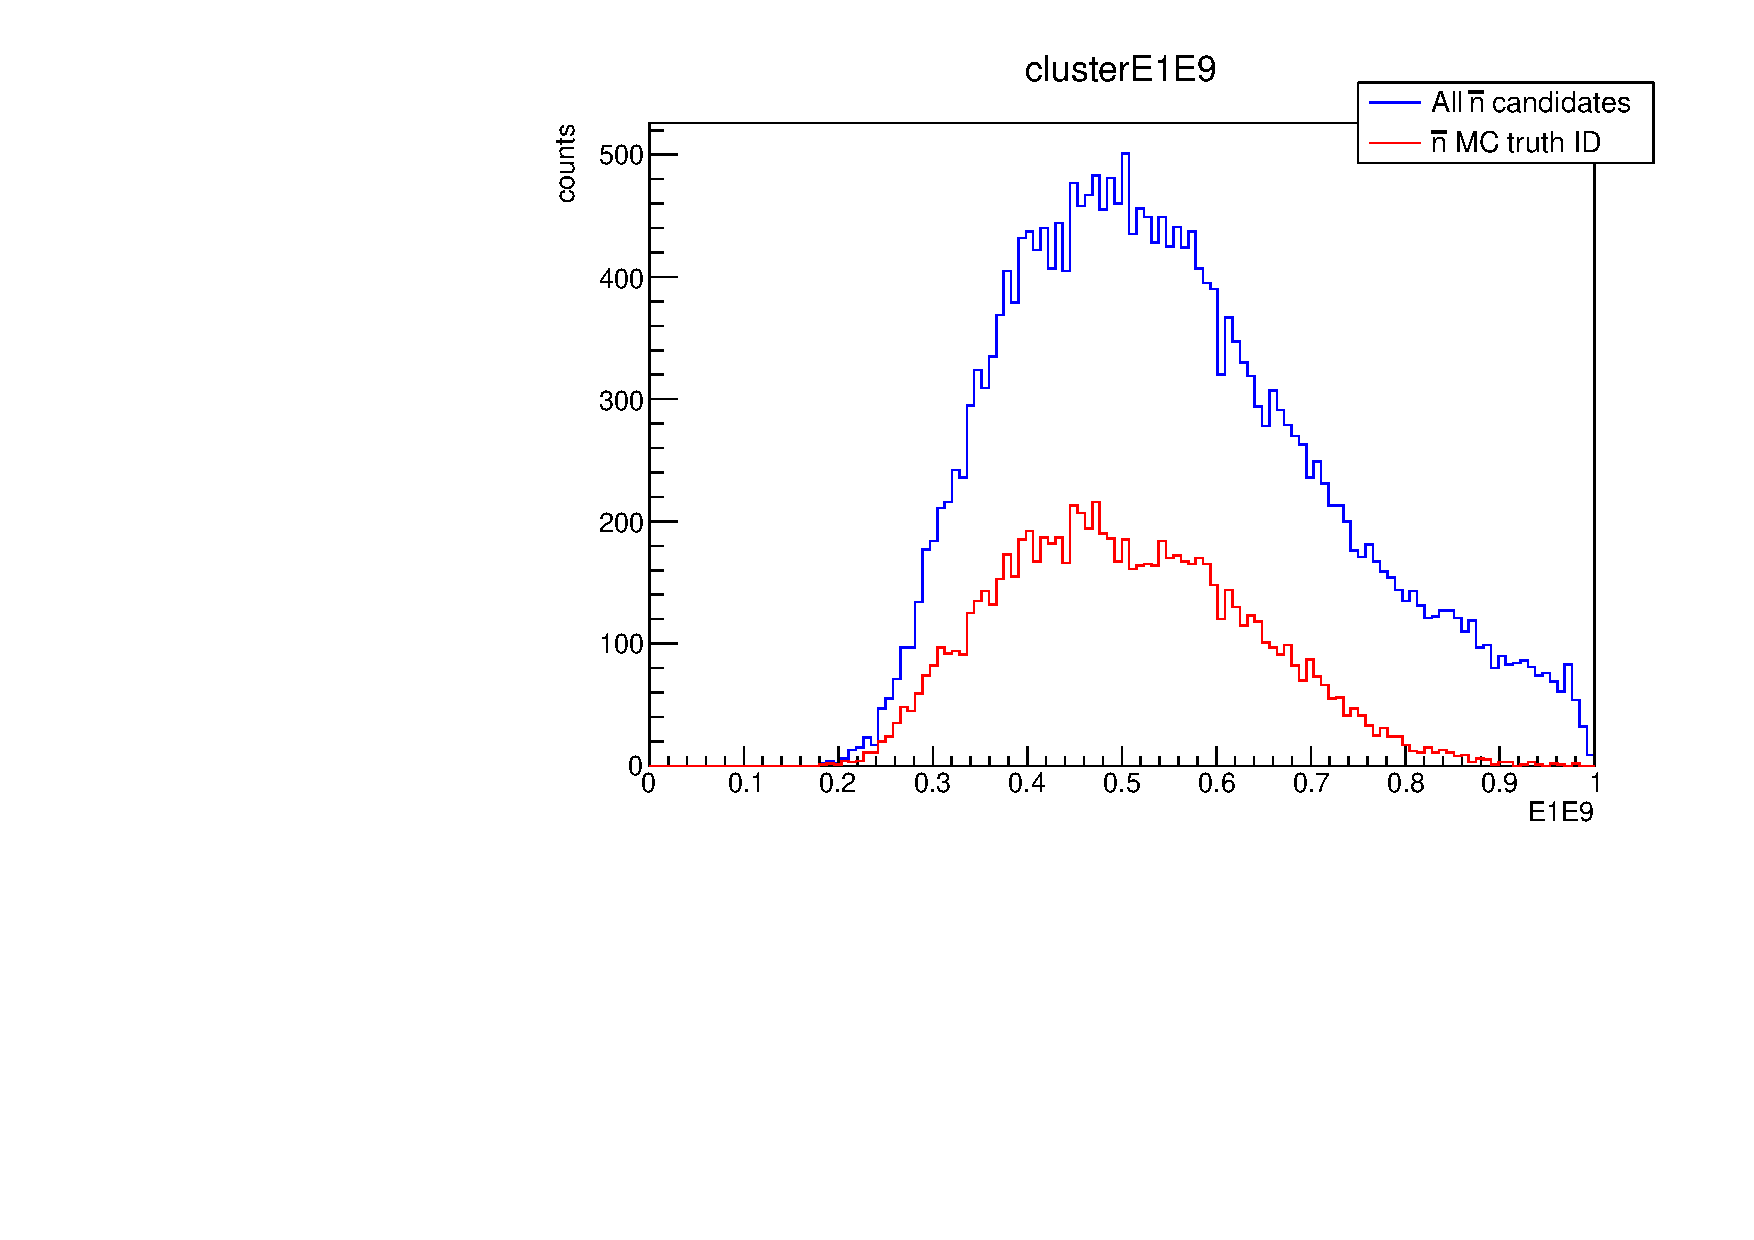
\includegraphics[width=0.49\textwidth]{nbar_MC/images/clusterE1E9_nog.pdf}
    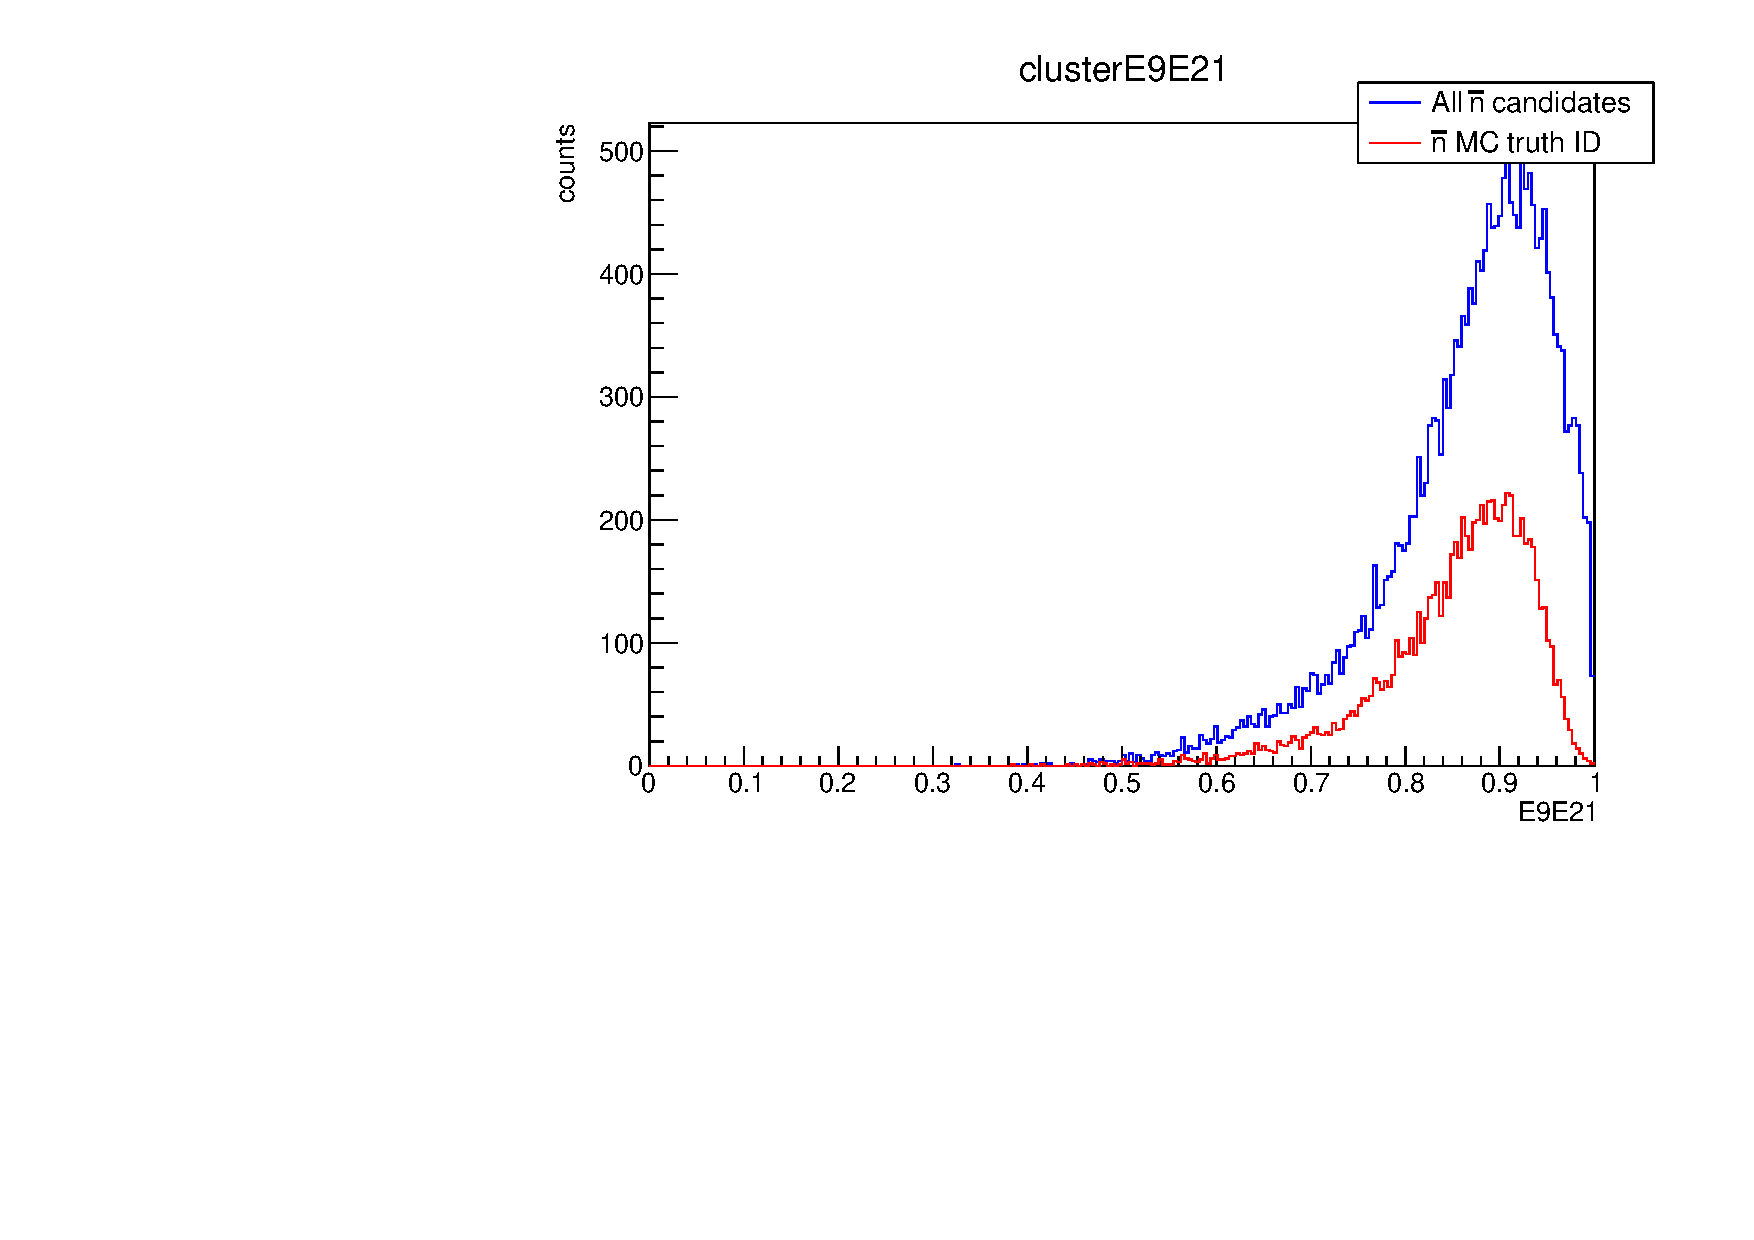
\includegraphics[width=0.49\textwidth]{nbar_MC/images/clusterE9E21_nog.pdf}
    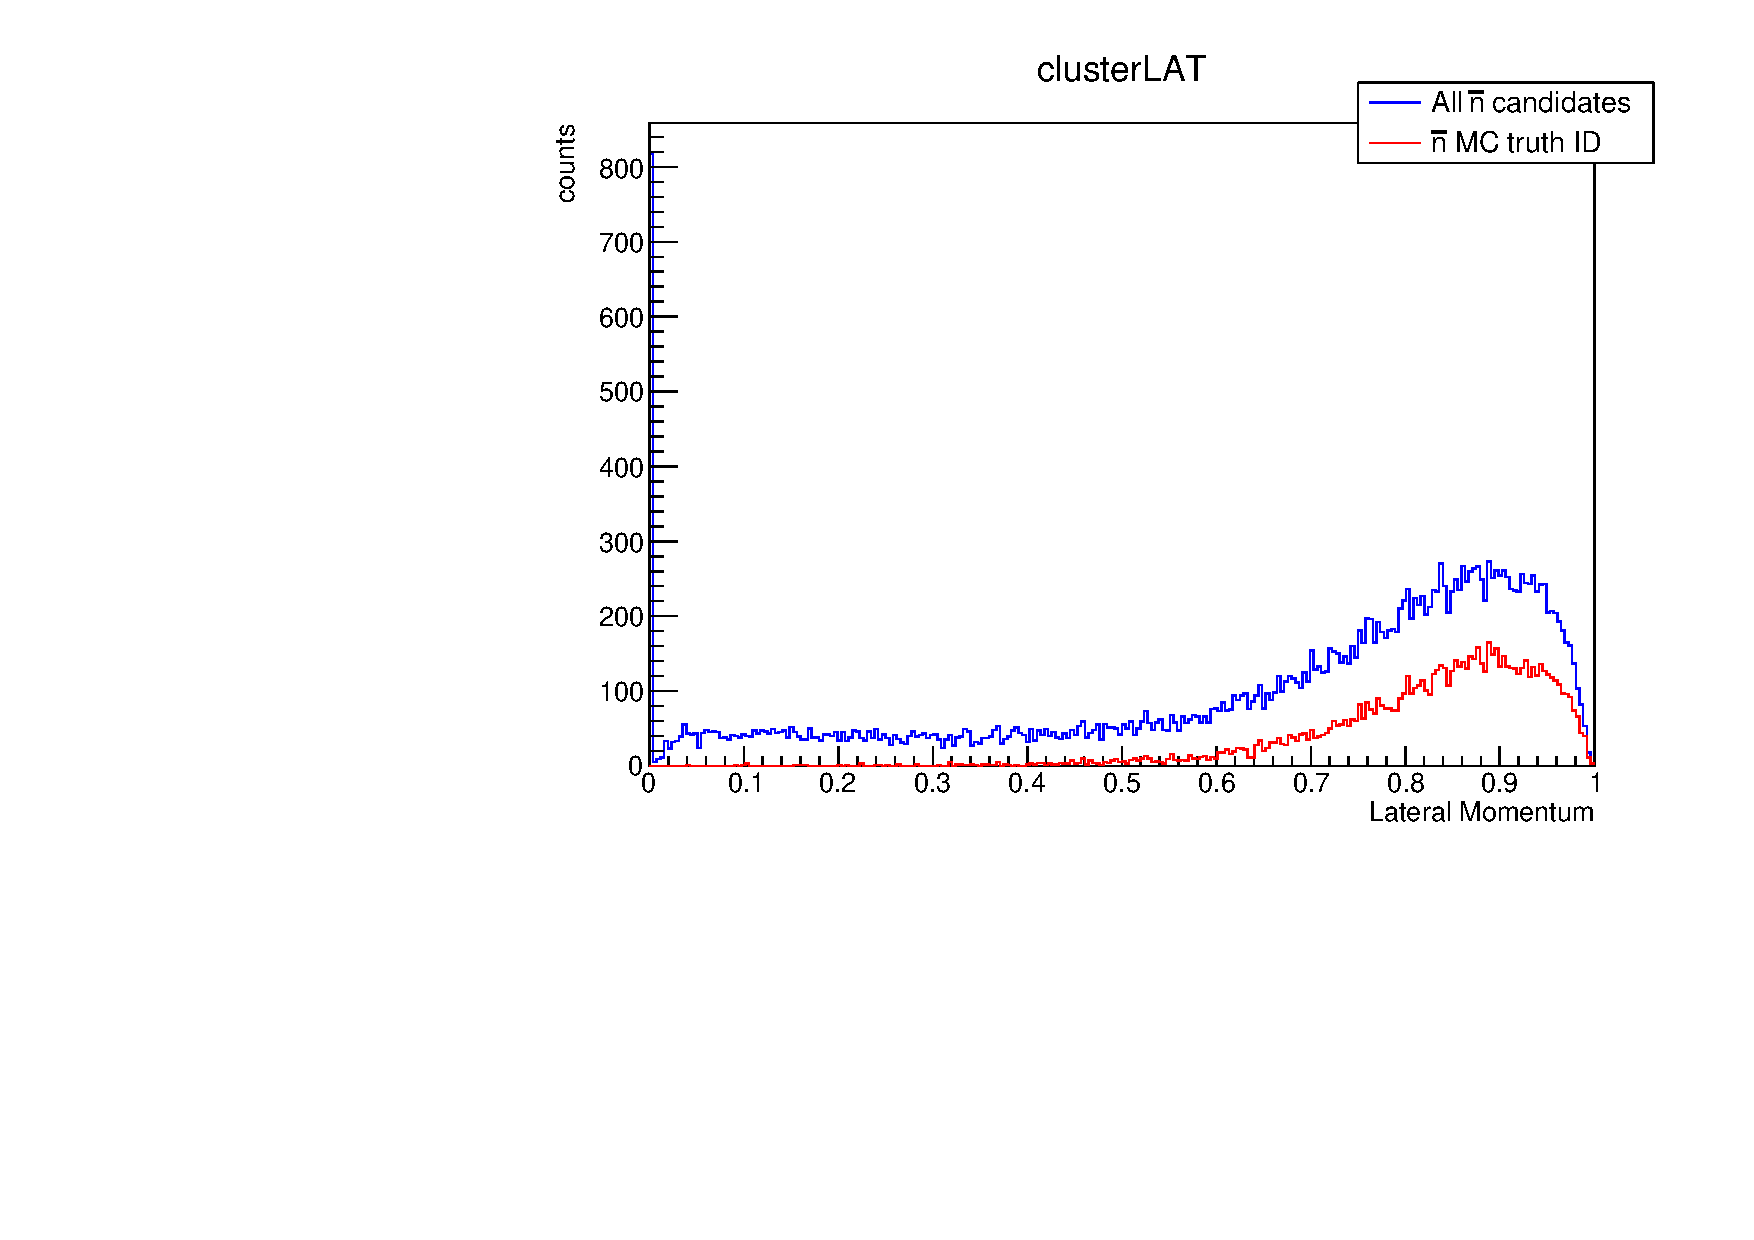
\includegraphics[width=0.49\textwidth]{nbar_MC/images/clusterLAT_nog.pdf}
    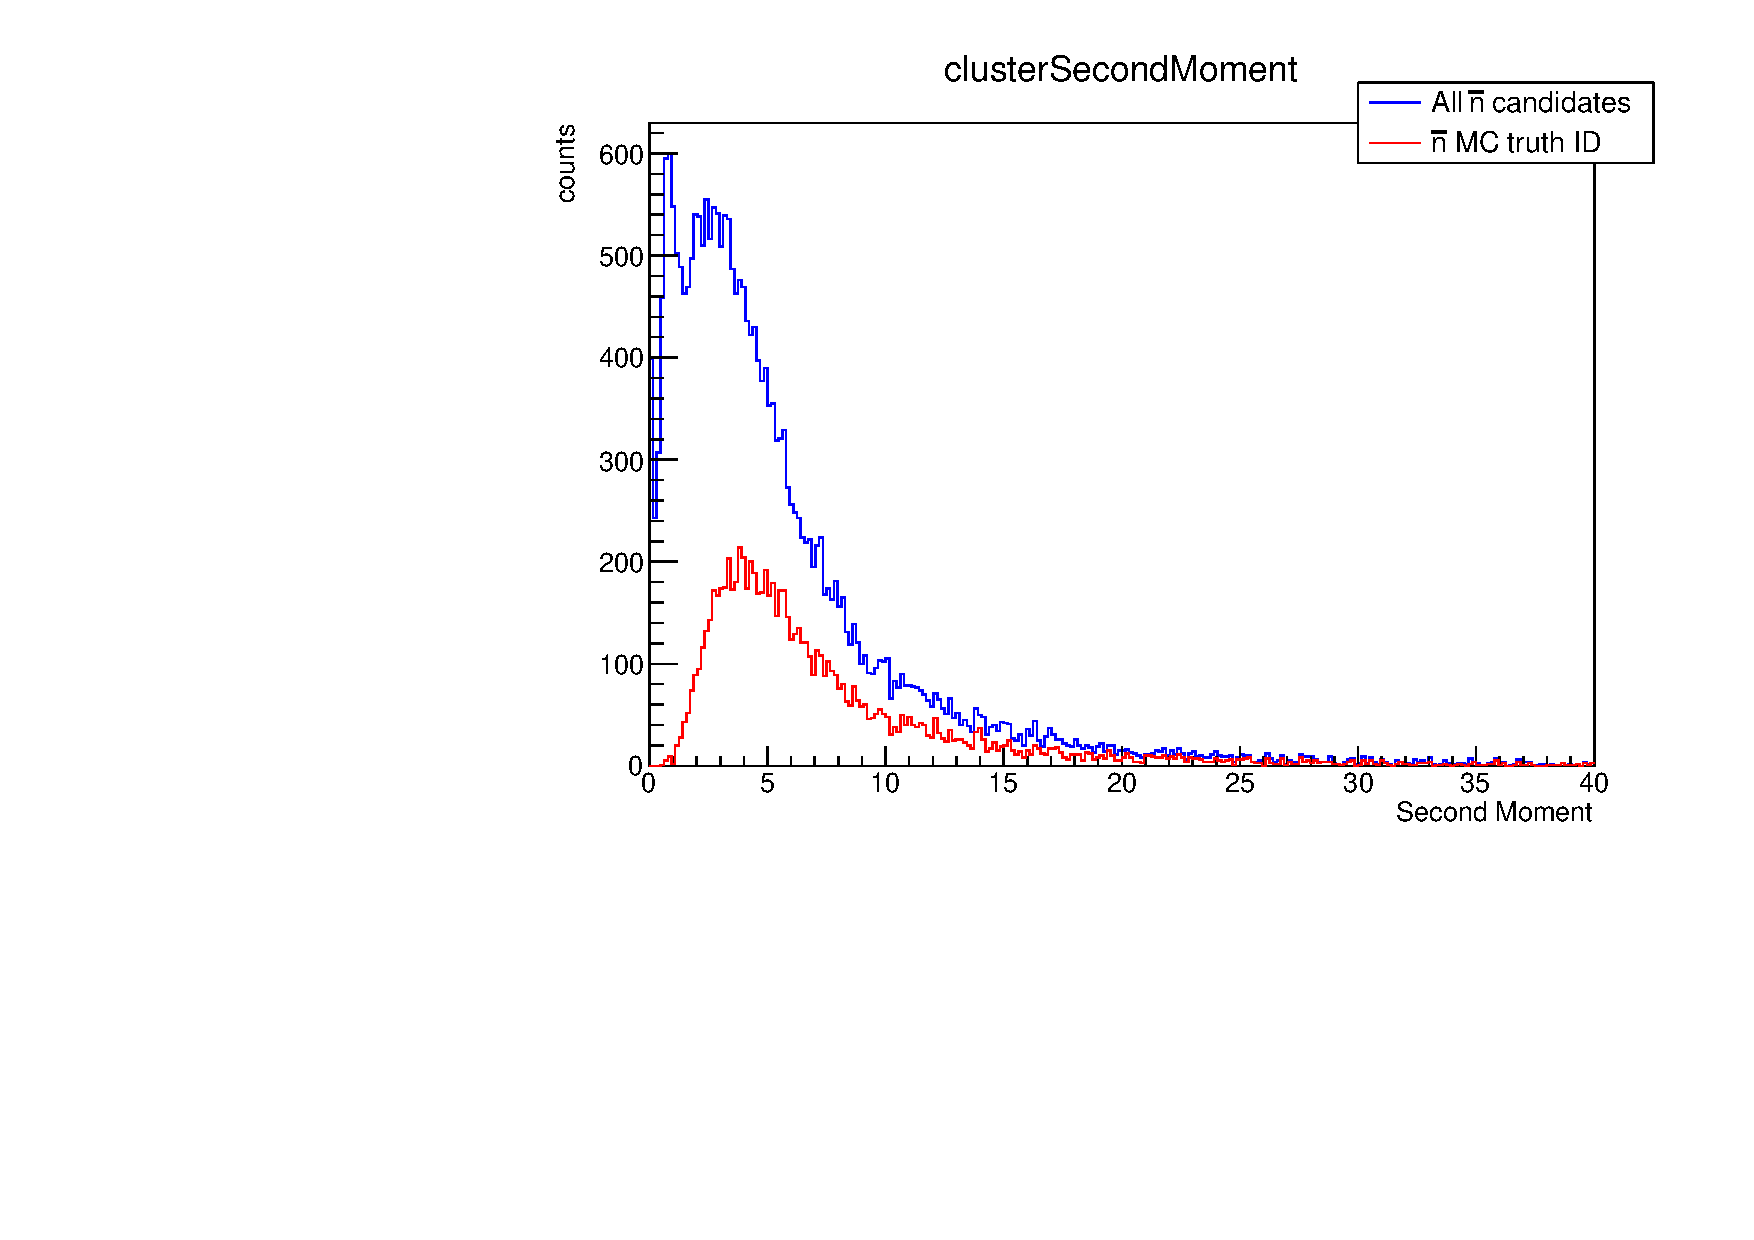
\includegraphics[width=0.49\textwidth]{nbar_MC/images/clusterSecondMoment_nog.pdf}
    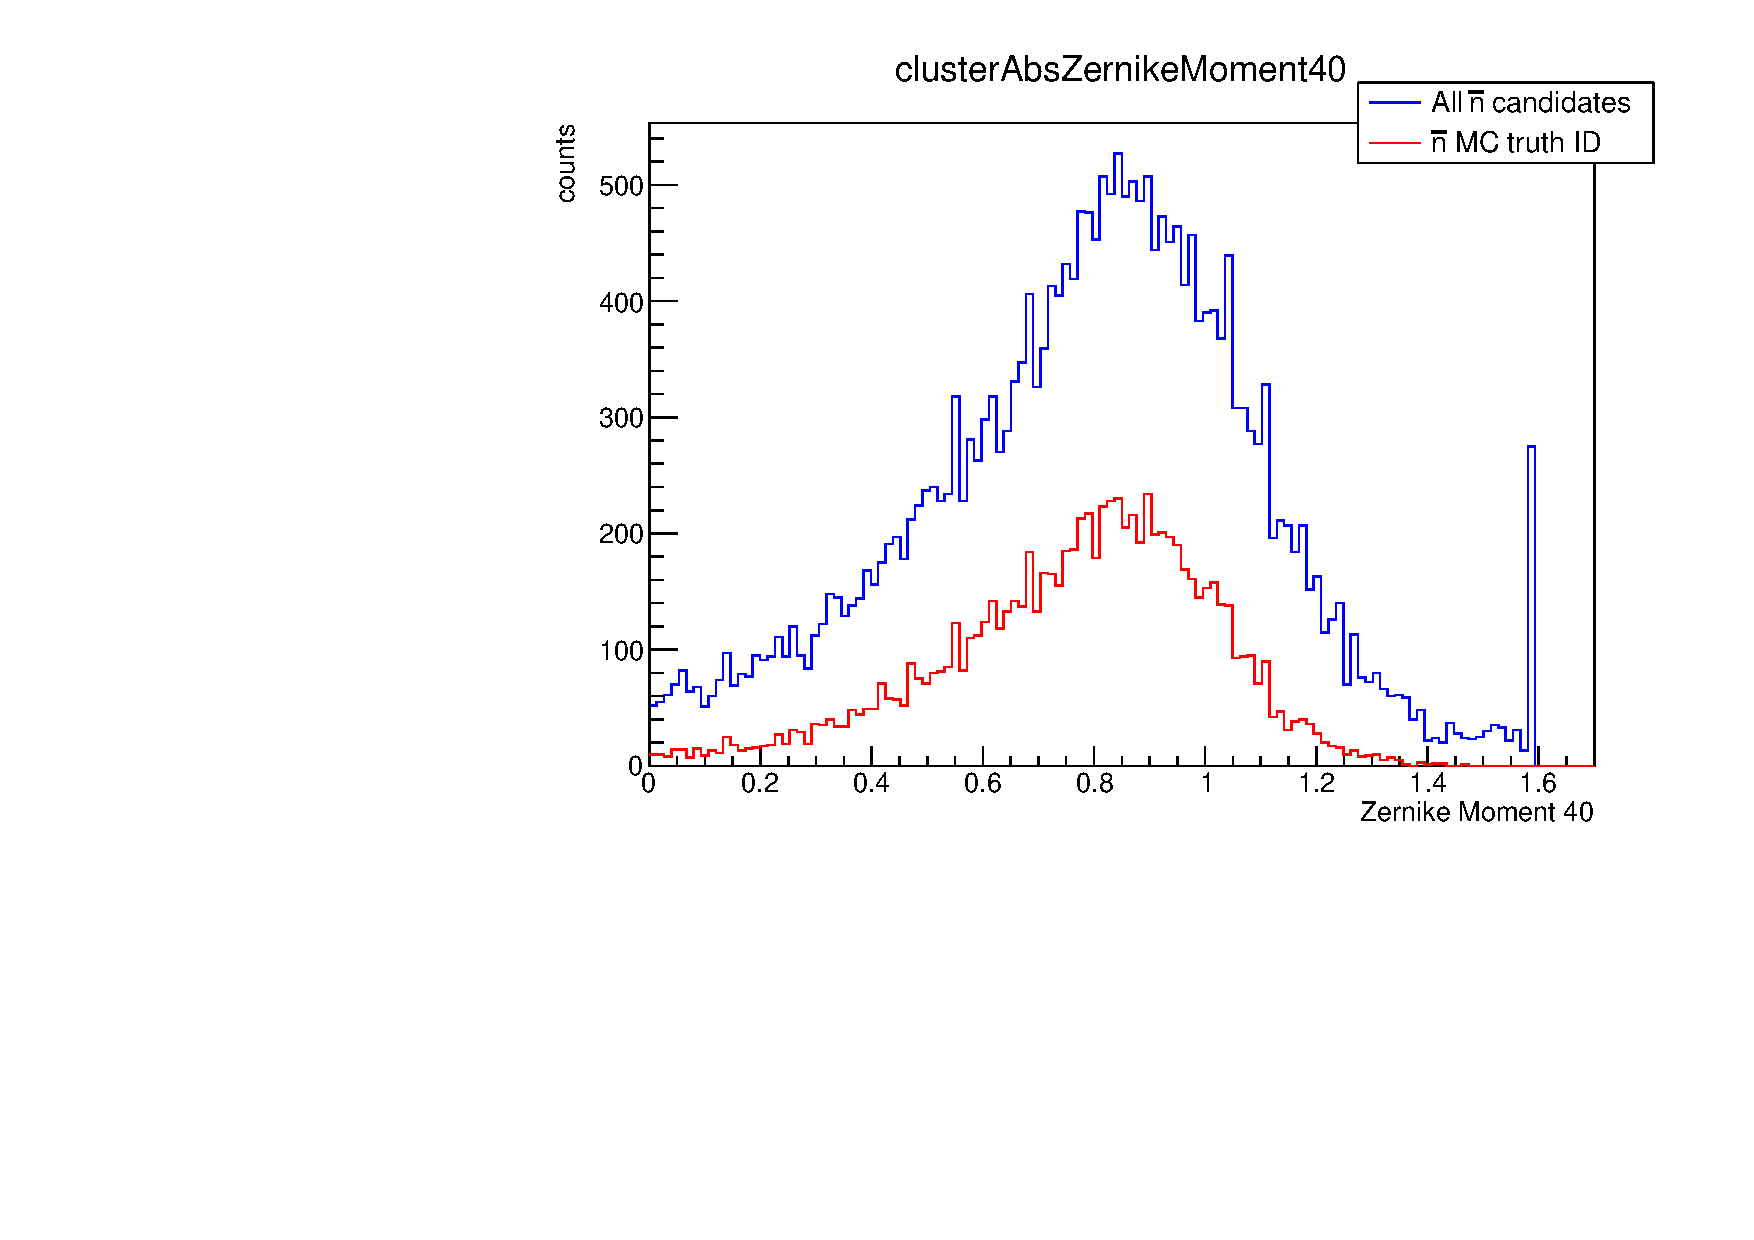
\includegraphics[width=0.49\textwidth]{nbar_MC/images/clusterAbsZernikeMoment40_nog.pdf}
    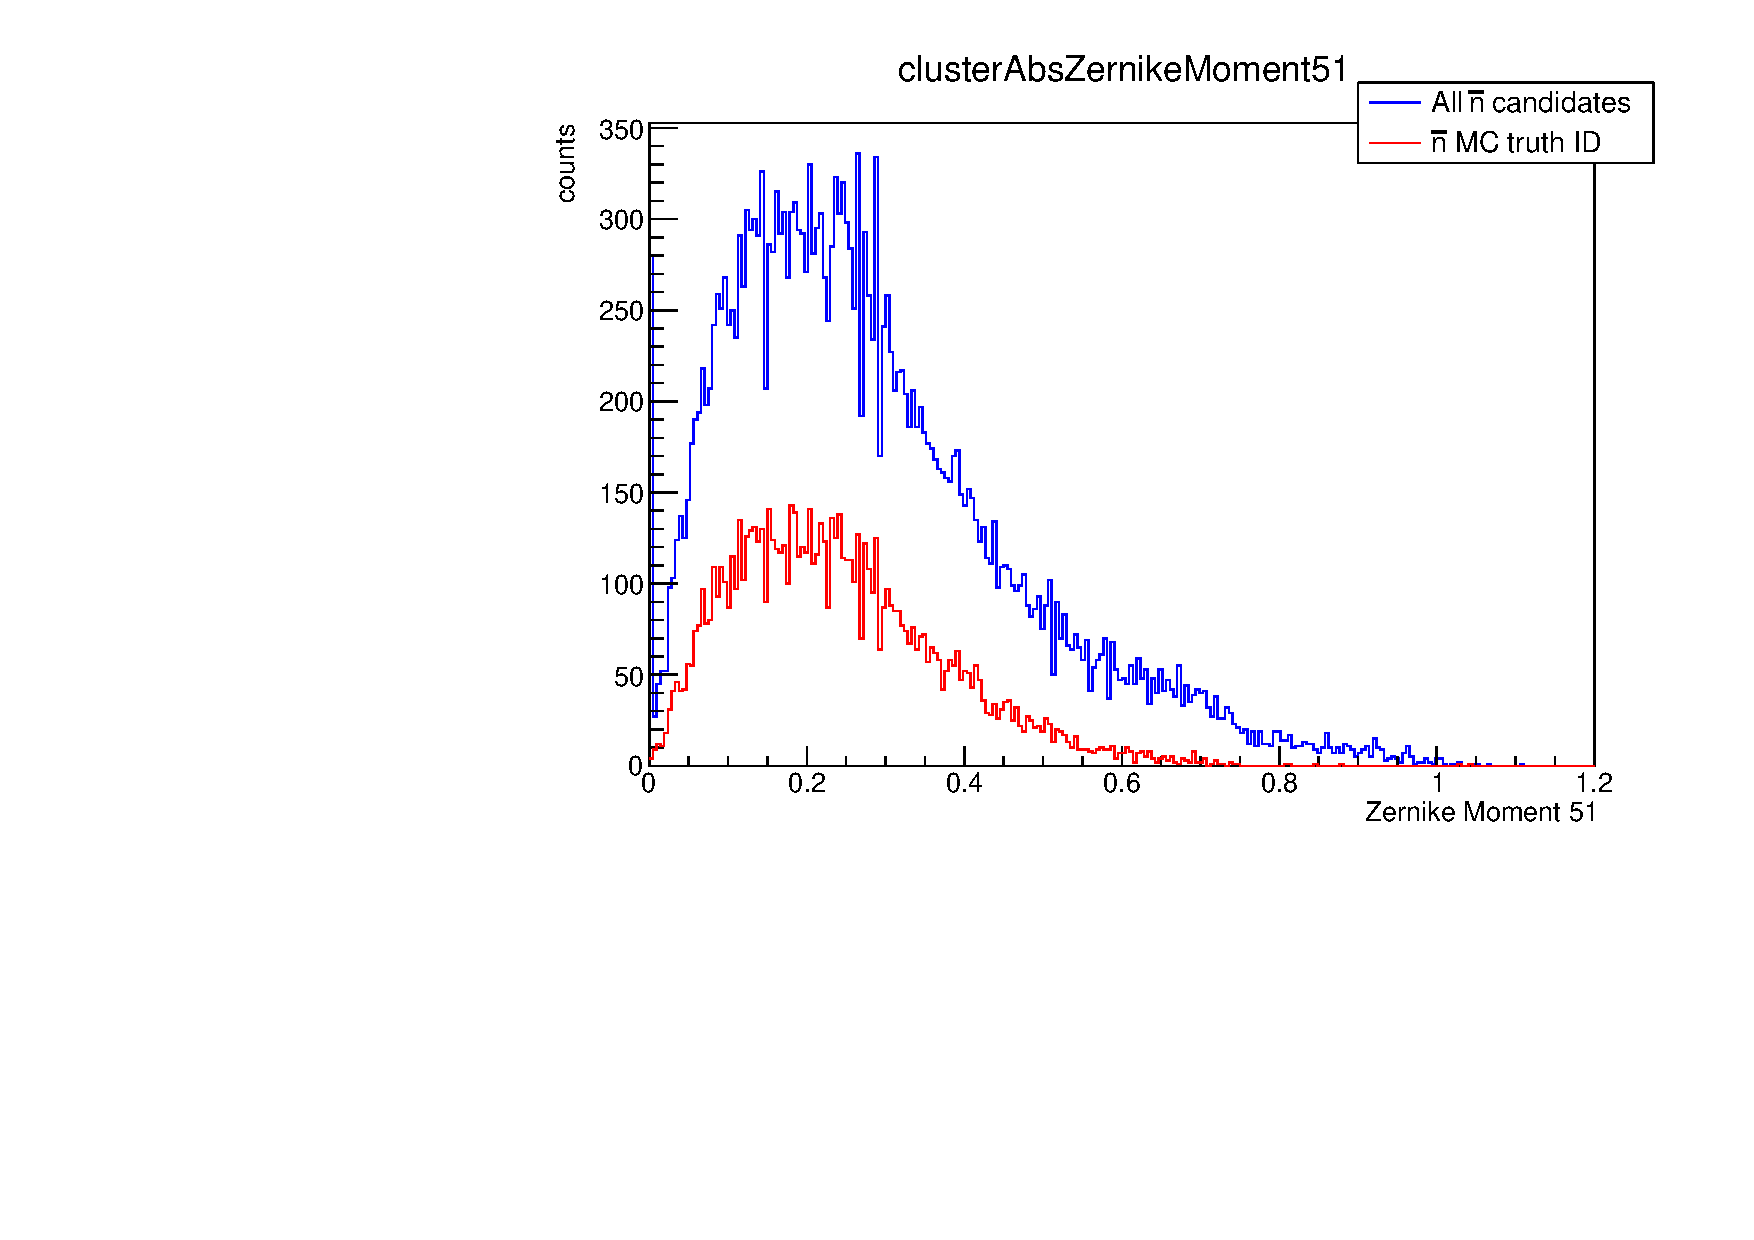
\includegraphics[width=0.49\textwidth]{nbar_MC/images/clusterAbsZernikeMoment51_nog.pdf}
    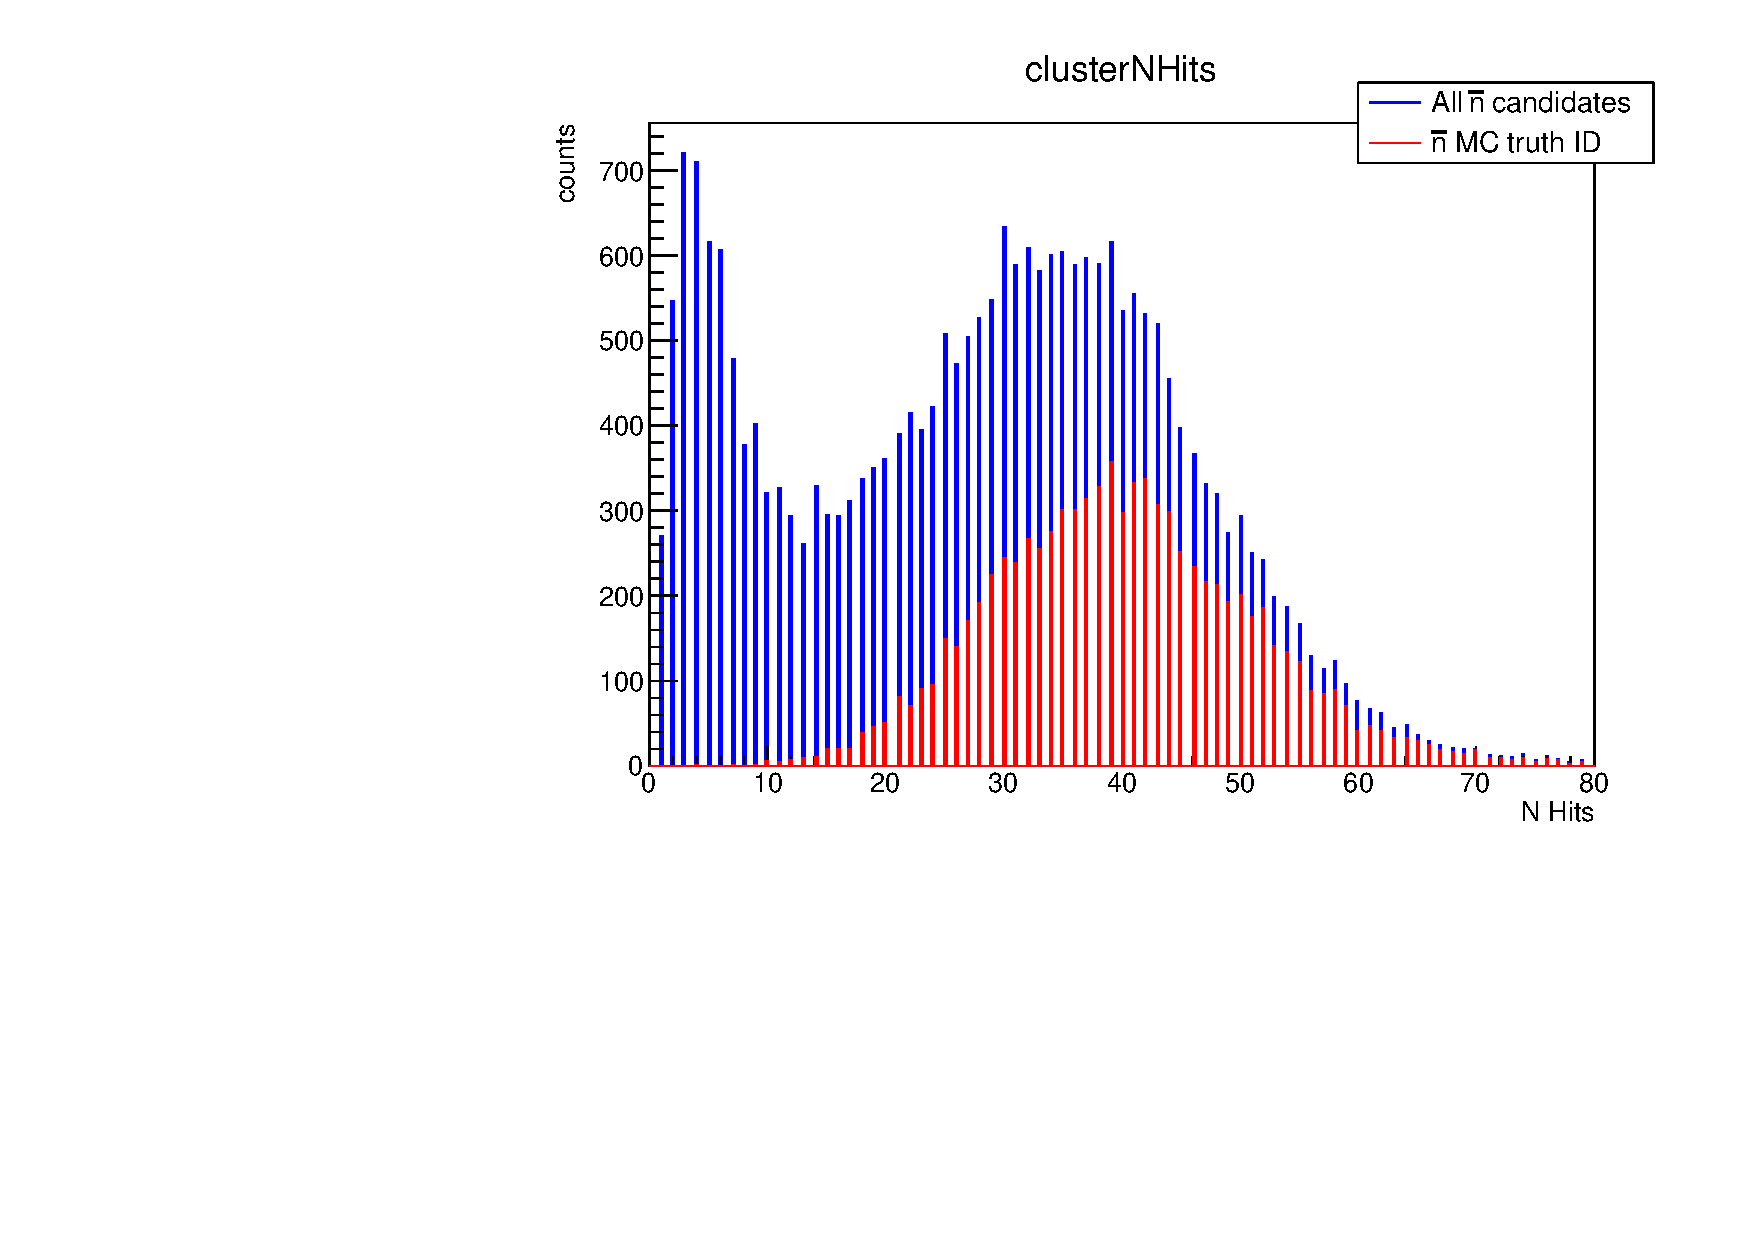
\includegraphics[width=0.49\textwidth]{nbar_MC/images/clusterNHits_nog.pdf}
   
     \caption{Comparison of reconstructed cluster variables for all $\bar{n}$ candidates versus those associated with $\bar{n}$ particles by Monte Carlo truth Monte Carlo PDG = -2112 (NO ISR case). The selection is performed using the Monte Carlo PDG code ($-2112$), as previously discussed}

\end{figure}

\newpage
First, it is important to highlight that the ISR and non-ISR distributions carry the same information, as expected. Indeed, the measurement of cluster variables is independent of the recoil system, which could be made of either $p \pi^- \gamma_{ISR}$ or $p \pi^-$ respectively.
$\\$
It is also noteworthy that the {\color{blue} blue distribution} shows some peculiar structures respect the {\color{red} red distribution}. The reconstructed cluster energy for all $\bar{n}$ candidates exhibits a first structure at low energy values that resembles those discussed for the anti-neutron momentum distributions. This is also evident in the second moment distribution, where a low-energy structure is clearly visible. The most prominent difference appears in the number of hits ($N \ Hit$) distribution, where a distinct structure at $N \ Hit < 10$ is evident.
$\\$
The nature of these characteristic structures is analyzed in the following sub-paragraph.

\subsubsection{Ancestor cluster variables}
It would be interesting to investigate the nature of this structure using the same approach as before, namely studying the ancestor contributions. The shower shapes with the following selections are compared:
\begin{itemize}
\item $\bar{n}$ Monte Carlo PDG = -2112 (neutral clusters correctly associated with $\bar{n}$ particles)
\item $\bar{n}$ Monte Carlo PDG = NaN (neutral clusters not associated with any particles)
\item $\bar{n}$ hasAncestor = 0 (neutral clusters with no $\bar{n}$ as relative)
\item $\bar{n}$ hasAncestor != 0 (neutral clusters with $\bar{n}$ as relative)
\end{itemize}

Referring to figures ~\ref{fig:cluster_ISR} and ~\ref{fig:cluster_NOISR}, as expected the neutral clusters correctly associated with $\bar{n}$ particles carry the same information of those without $\bar{n}$ as relative, in bot ISR and NO ISR cases.
$\\$
Furthermore, it is evident how reconstructed neutral clusters not associated with any particles by the Monte Carlo and those with $\bar{n}$ as relative are primarily responsible for the structures observed at low values of energy, second moment, and number of crystals.
$\\$
A further selection on number of crystals ($clusterNHits > 10$) can be performed to study the corresponding cluster variables. The result is shown in figure  ~\ref{fig:cluster_ISR_NHits} and ~\ref{fig:cluster_NOISR_NHits}. 
$\\$
As observed, these structures arise from small-sized clusters produced by $\bar{n}$ particles that undergo phenomena -such as cluster split-off and pre-showering- prior to neutral cluster formation for $\bar{n}$ candidates, as confirmed by ancestor studies. The requirement of at least 10 crystals eliminates these structures.
\newpage
The obtained cluster variables in  ISR case are shown below:
 \begin{figure}[H]
    \centering
    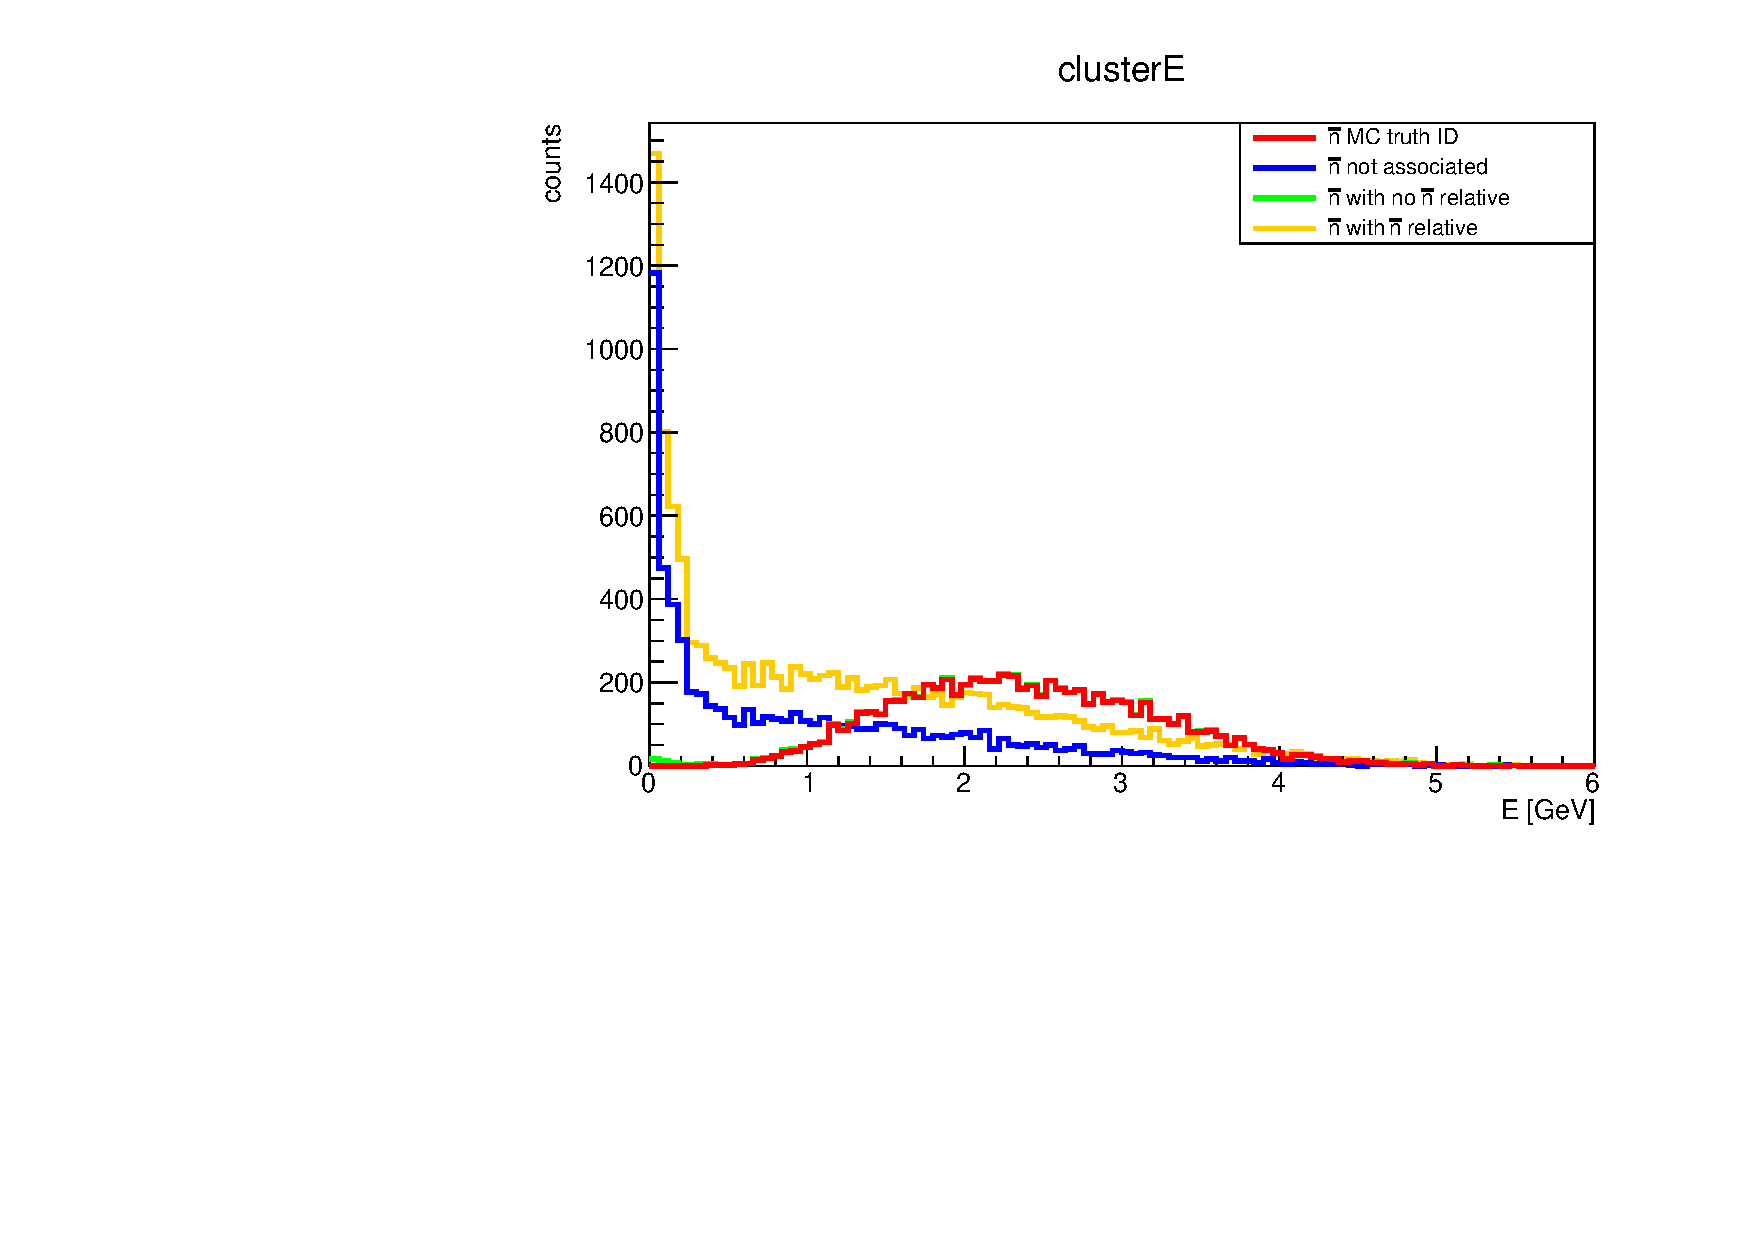
\includegraphics[width=0.49\textwidth]{nbar_MC/images/clusterE_isr_ancestor.pdf}
    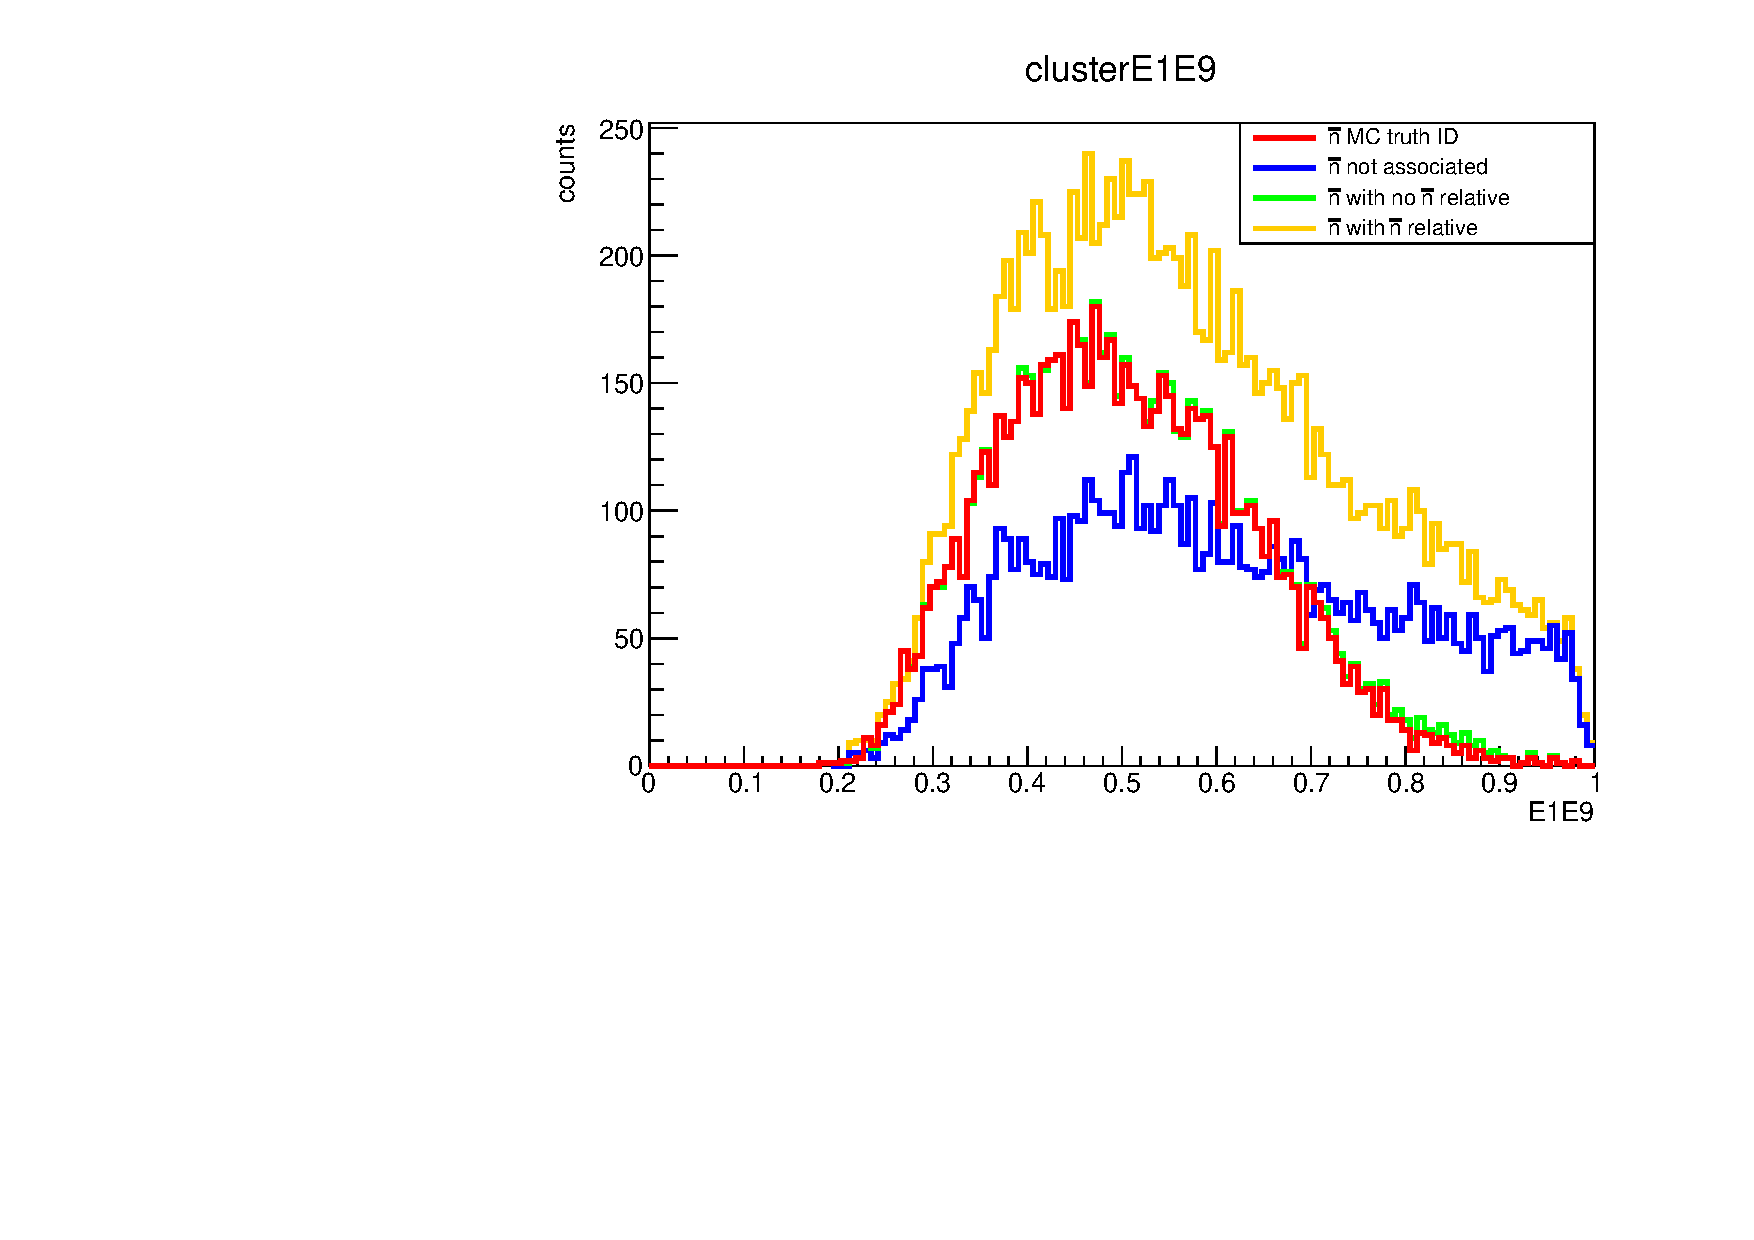
\includegraphics[width=0.49\textwidth]{nbar_MC/images/clusterE1E9_isr_ancestor.pdf}
    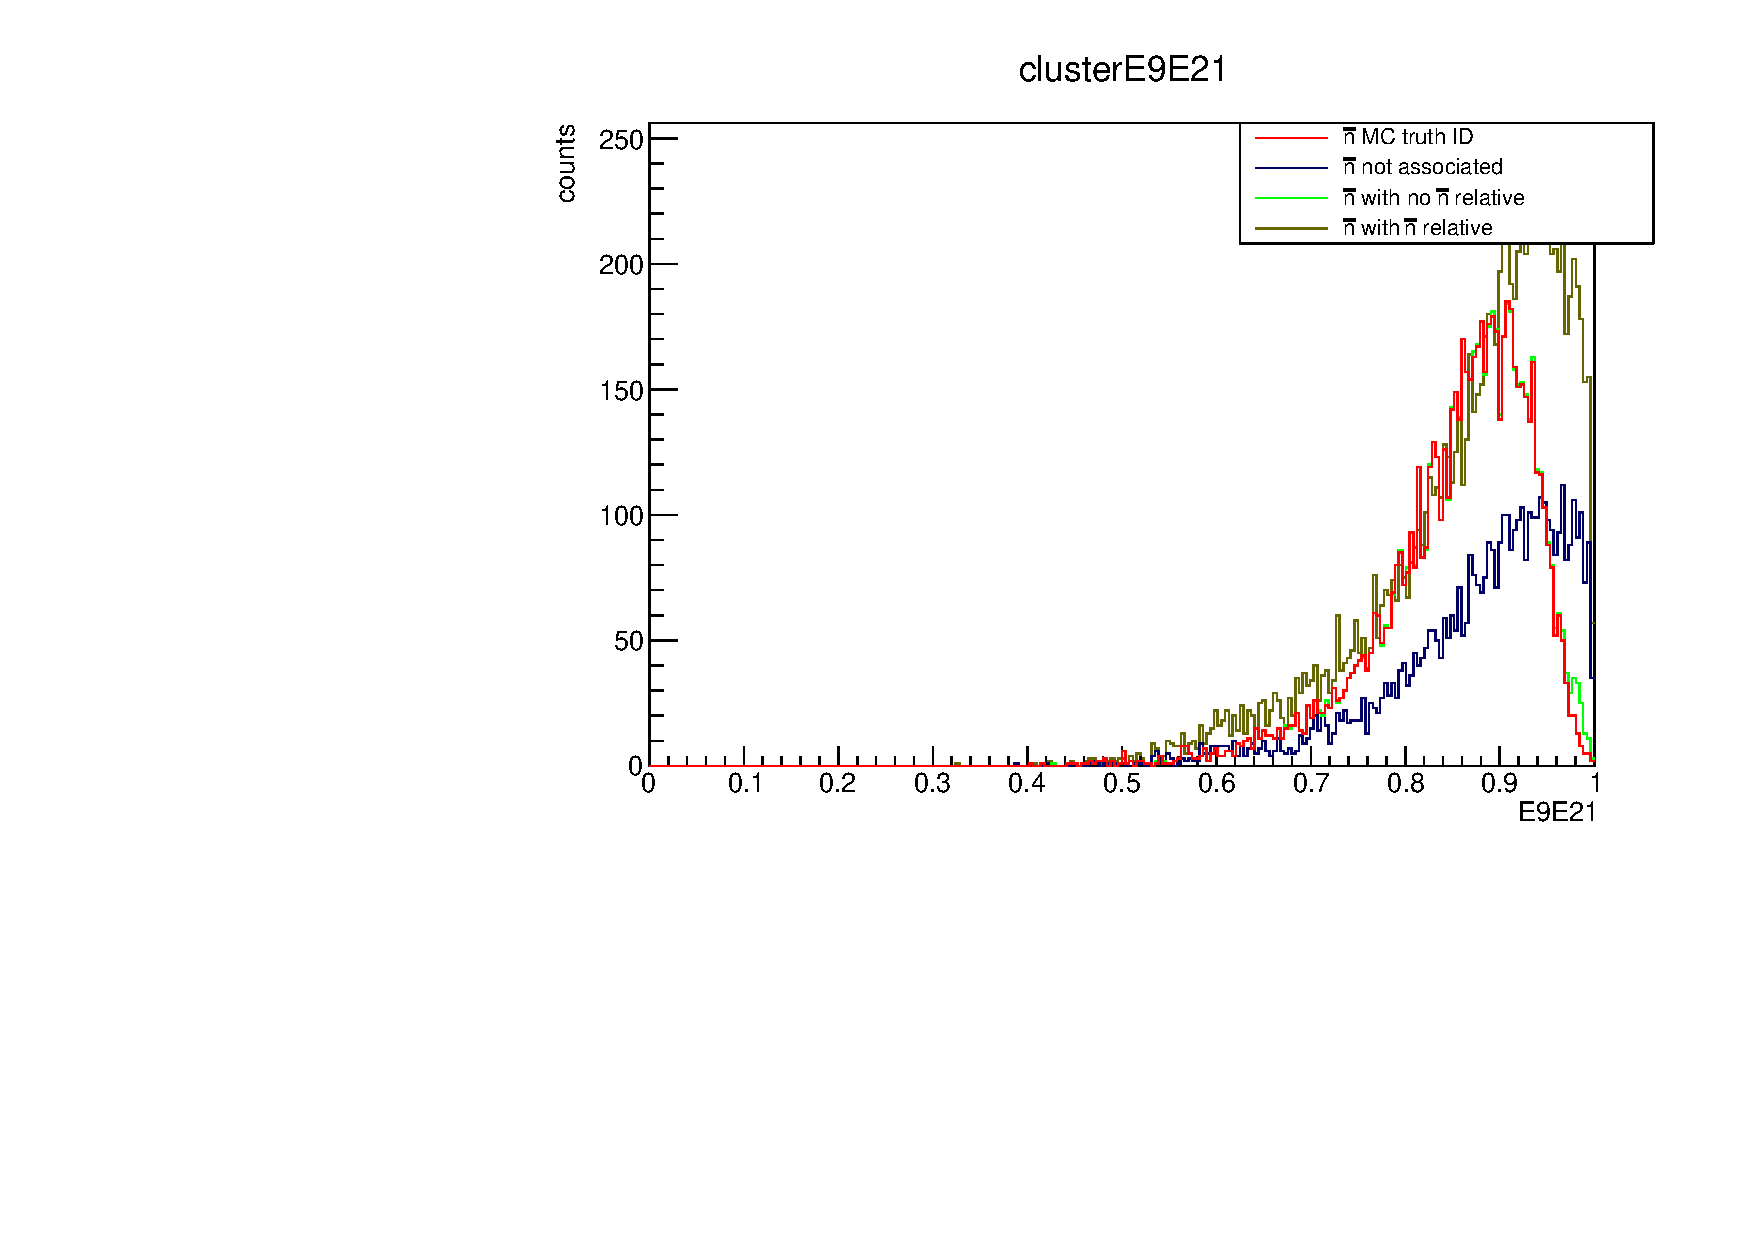
\includegraphics[width=0.49\textwidth]{nbar_MC/images/clusterE9E21_isr_ancestor.pdf}
    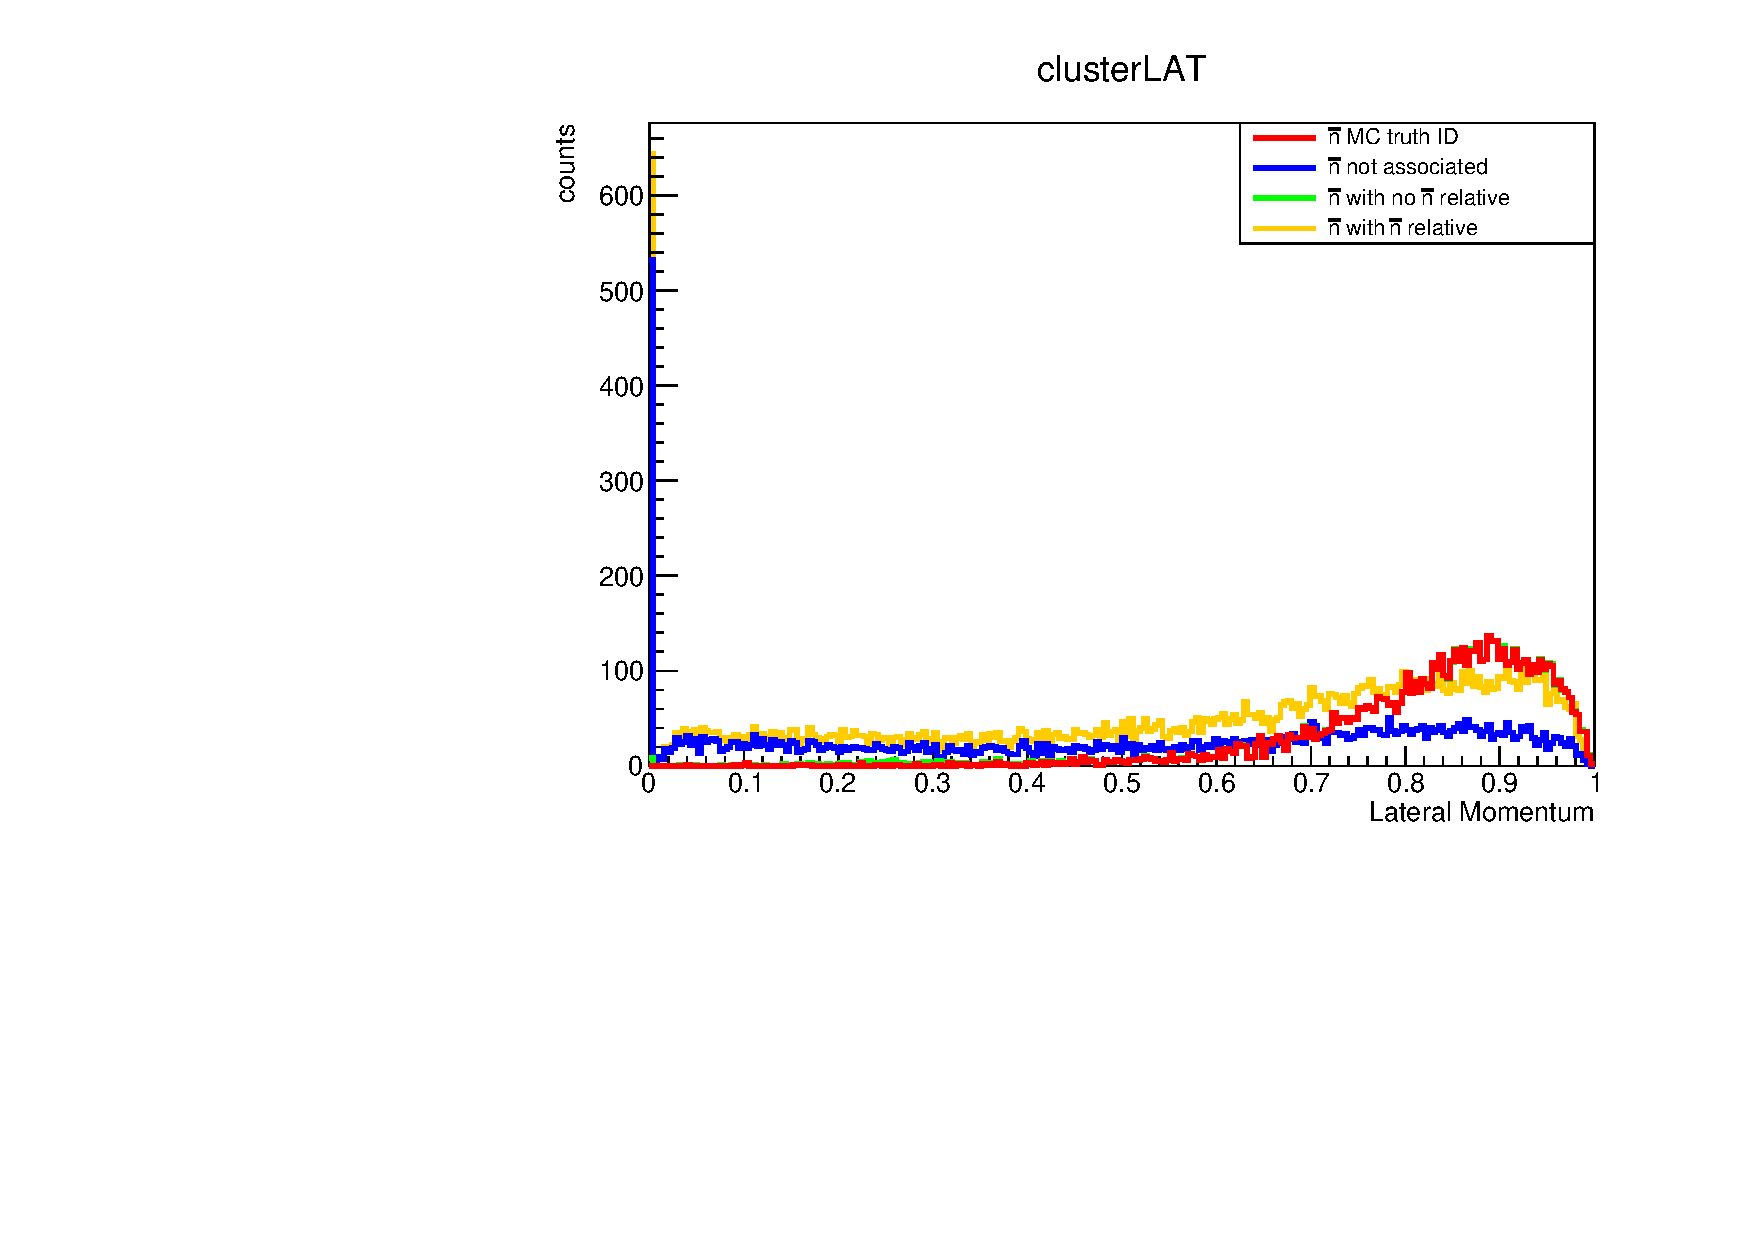
\includegraphics[width=0.49\textwidth]{nbar_MC/images/clusterLAT_isr_ancestor.pdf}
    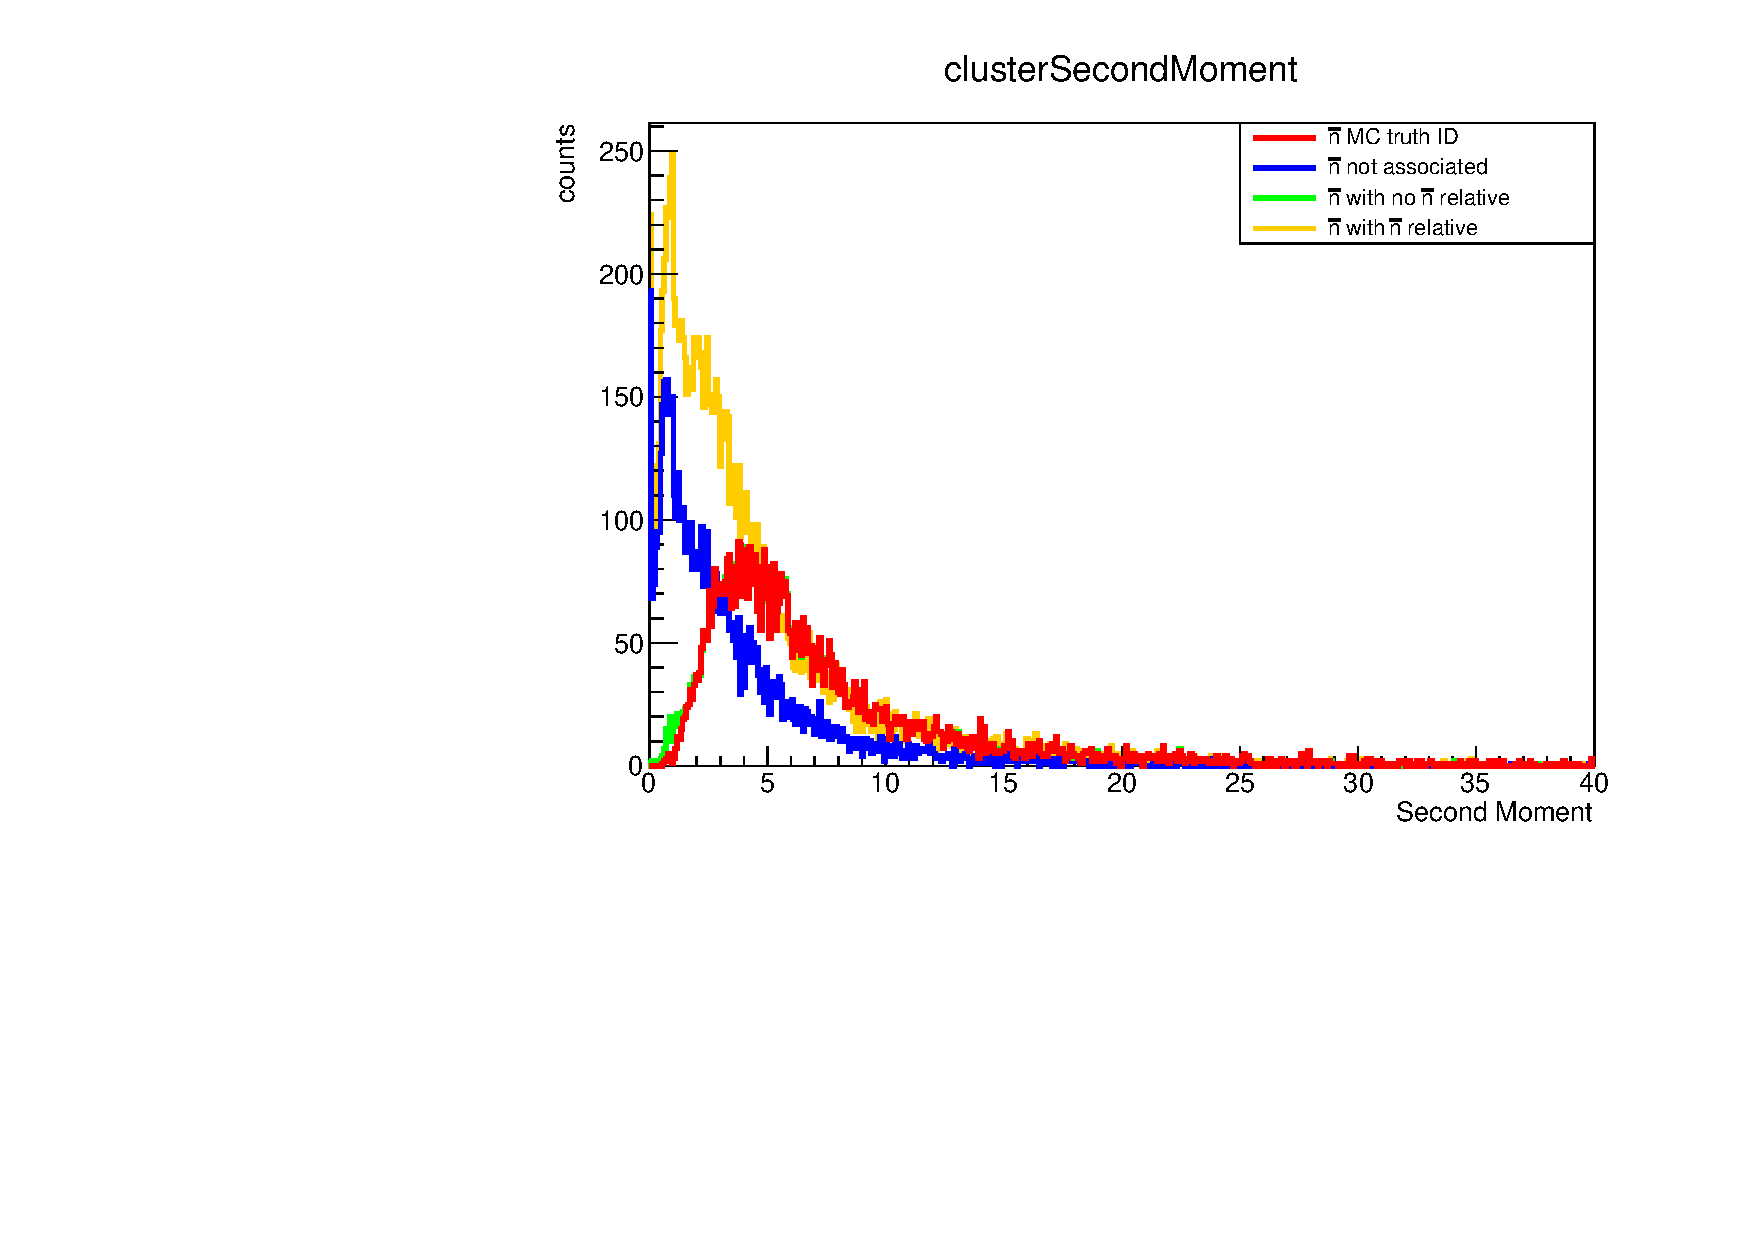
\includegraphics[width=0.49\textwidth]{nbar_MC/images/clusterSecondMoment_isr_ancestor.pdf}
    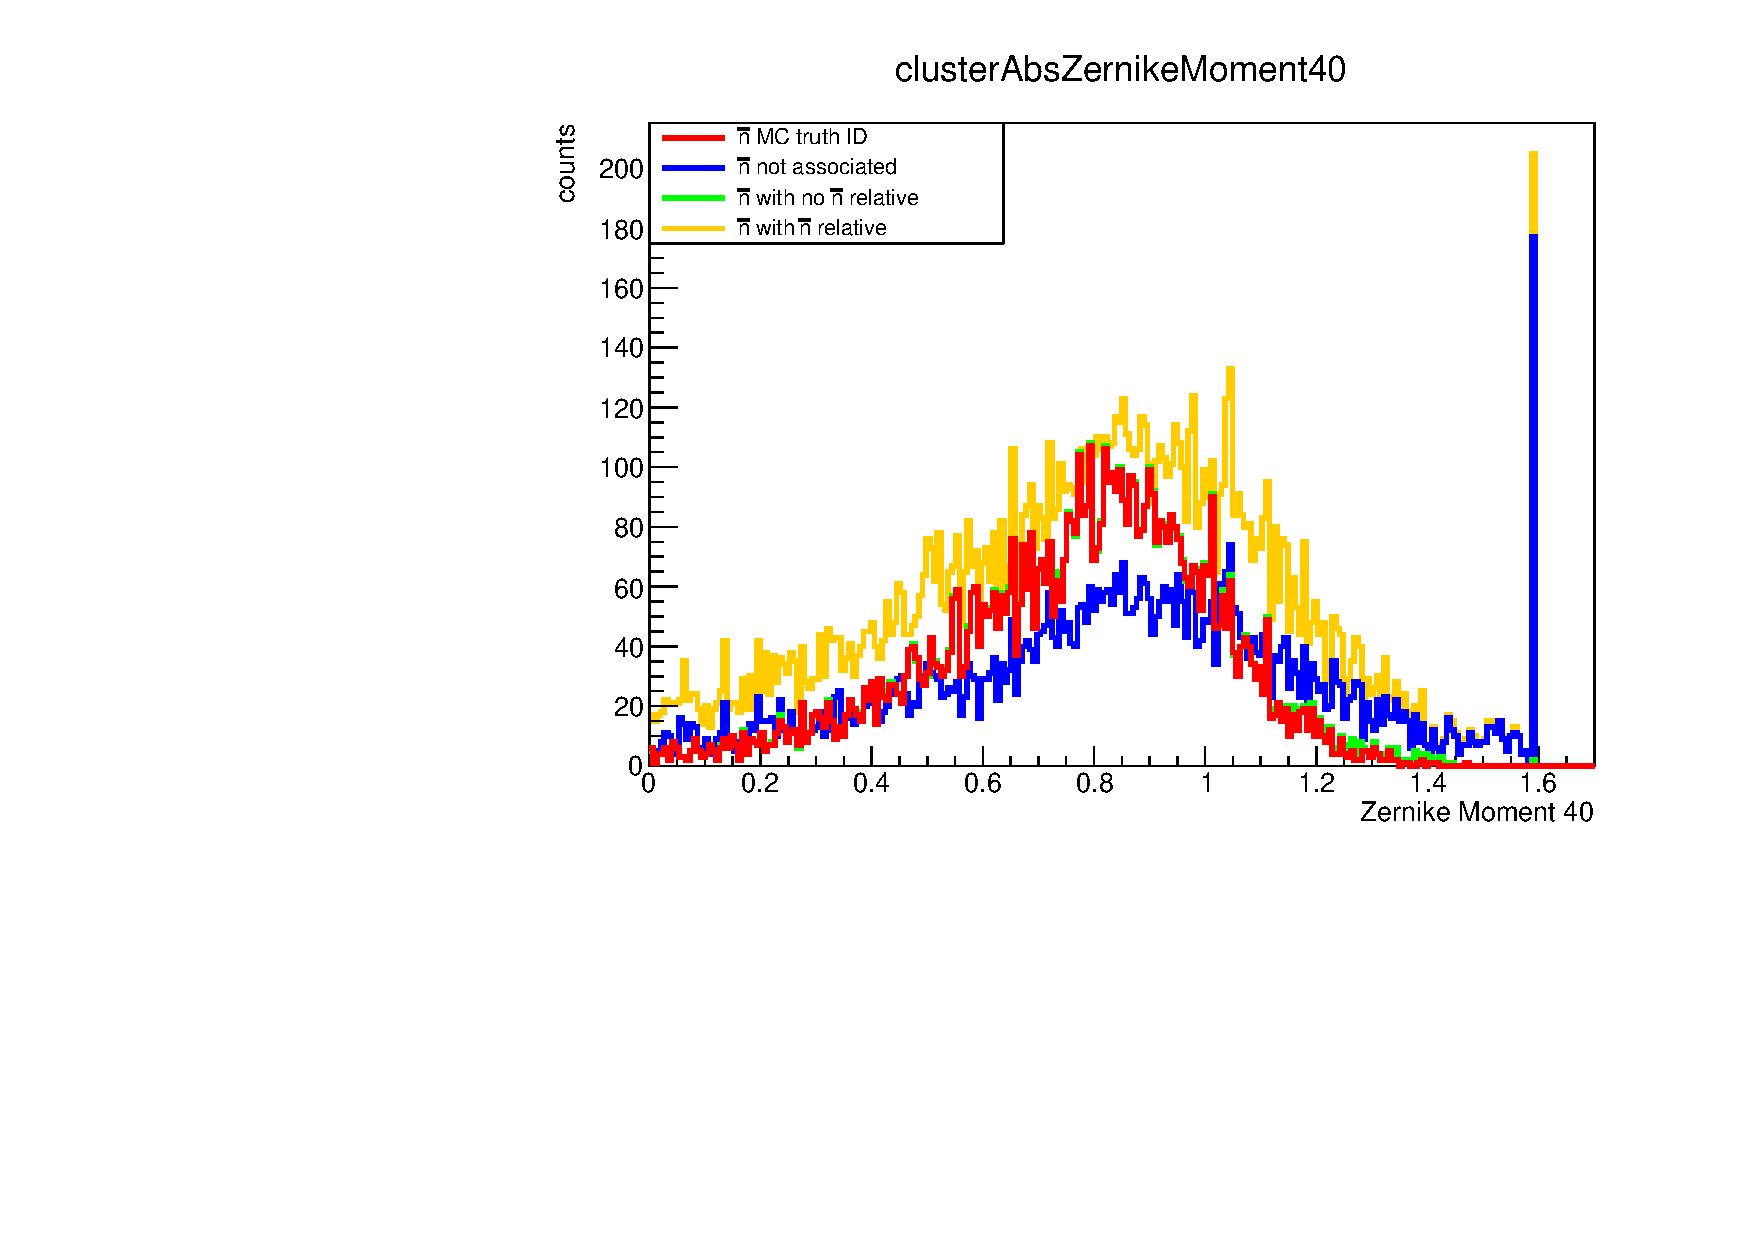
\includegraphics[width=0.49\textwidth]{nbar_MC/images/clusterAbsZernikeMoment40_isr_ancestor.pdf}
    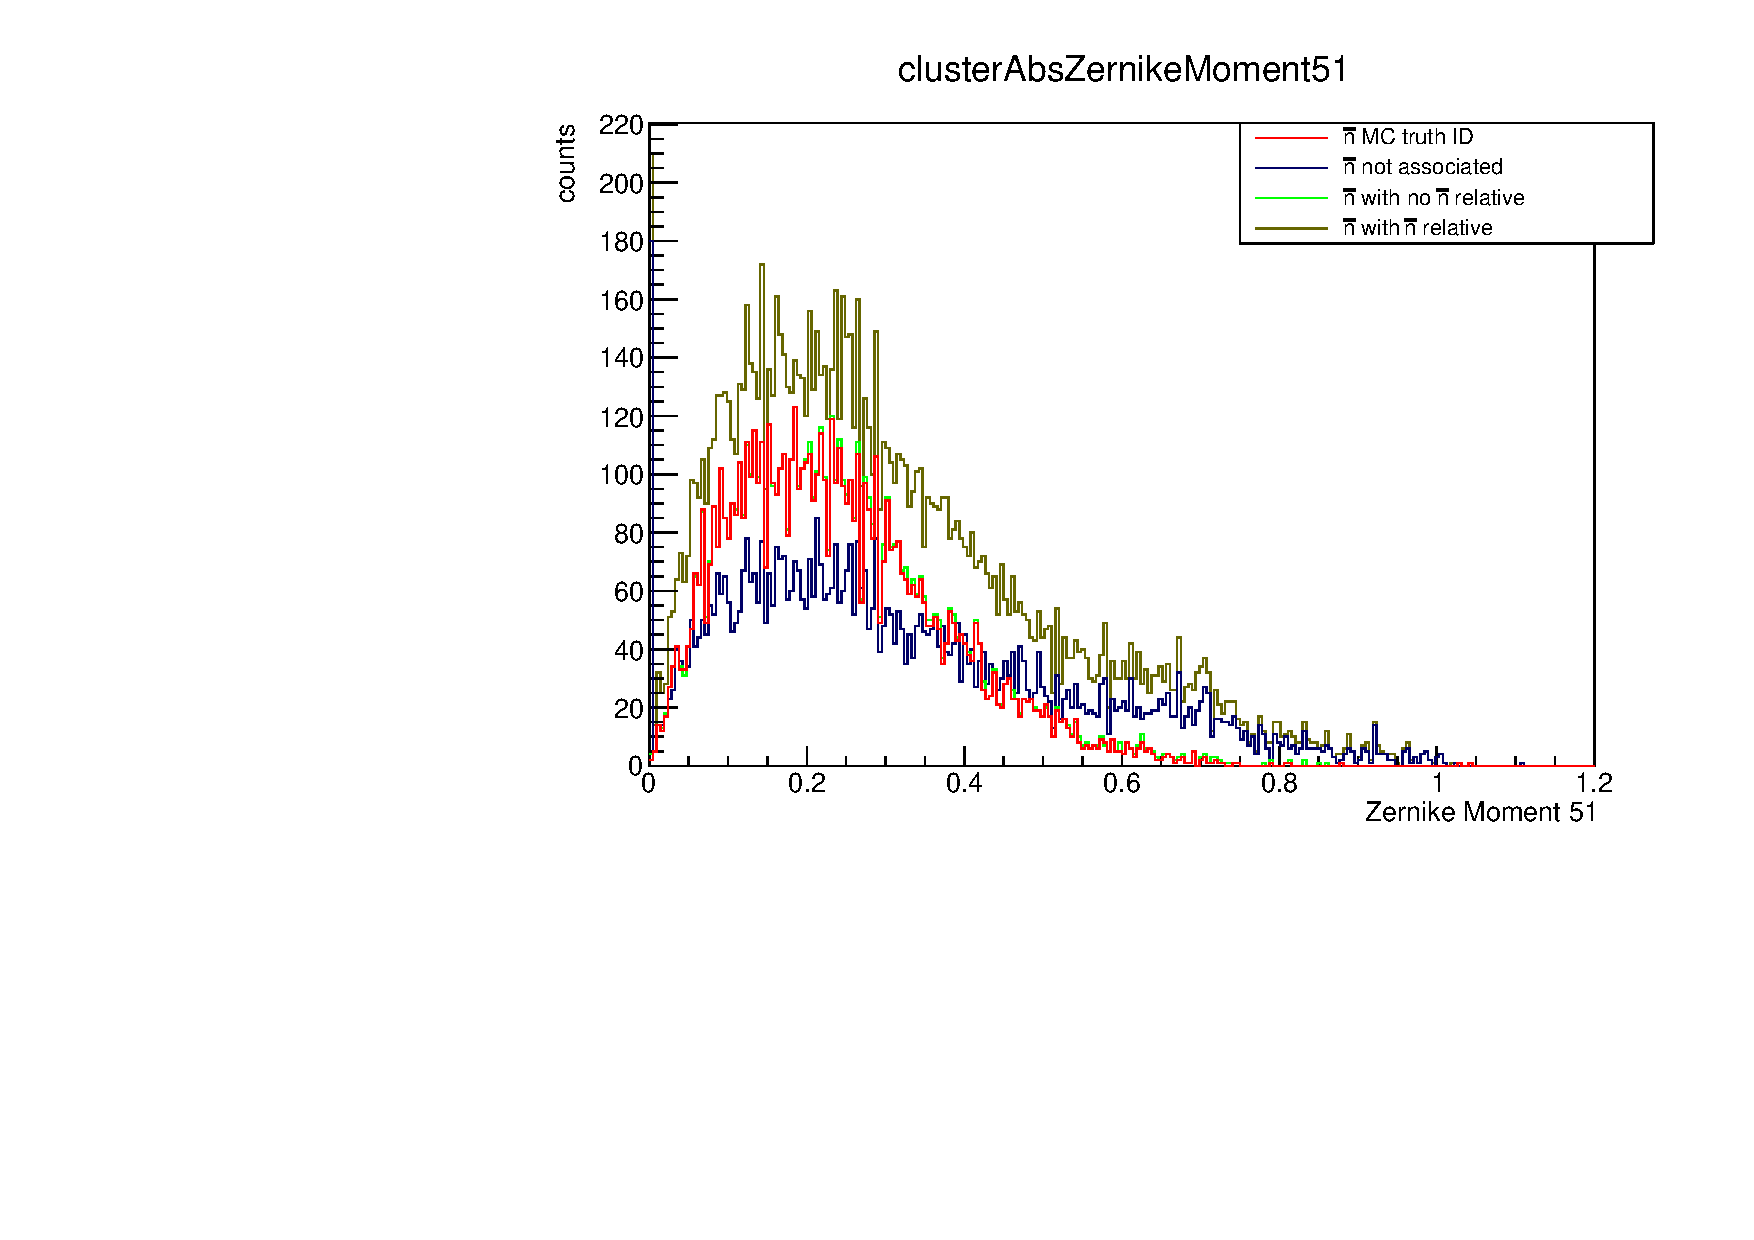
\includegraphics[width=0.49\textwidth]{nbar_MC/images/clusterAbsZernikeMoment51_isr_ancestor.pdf}
    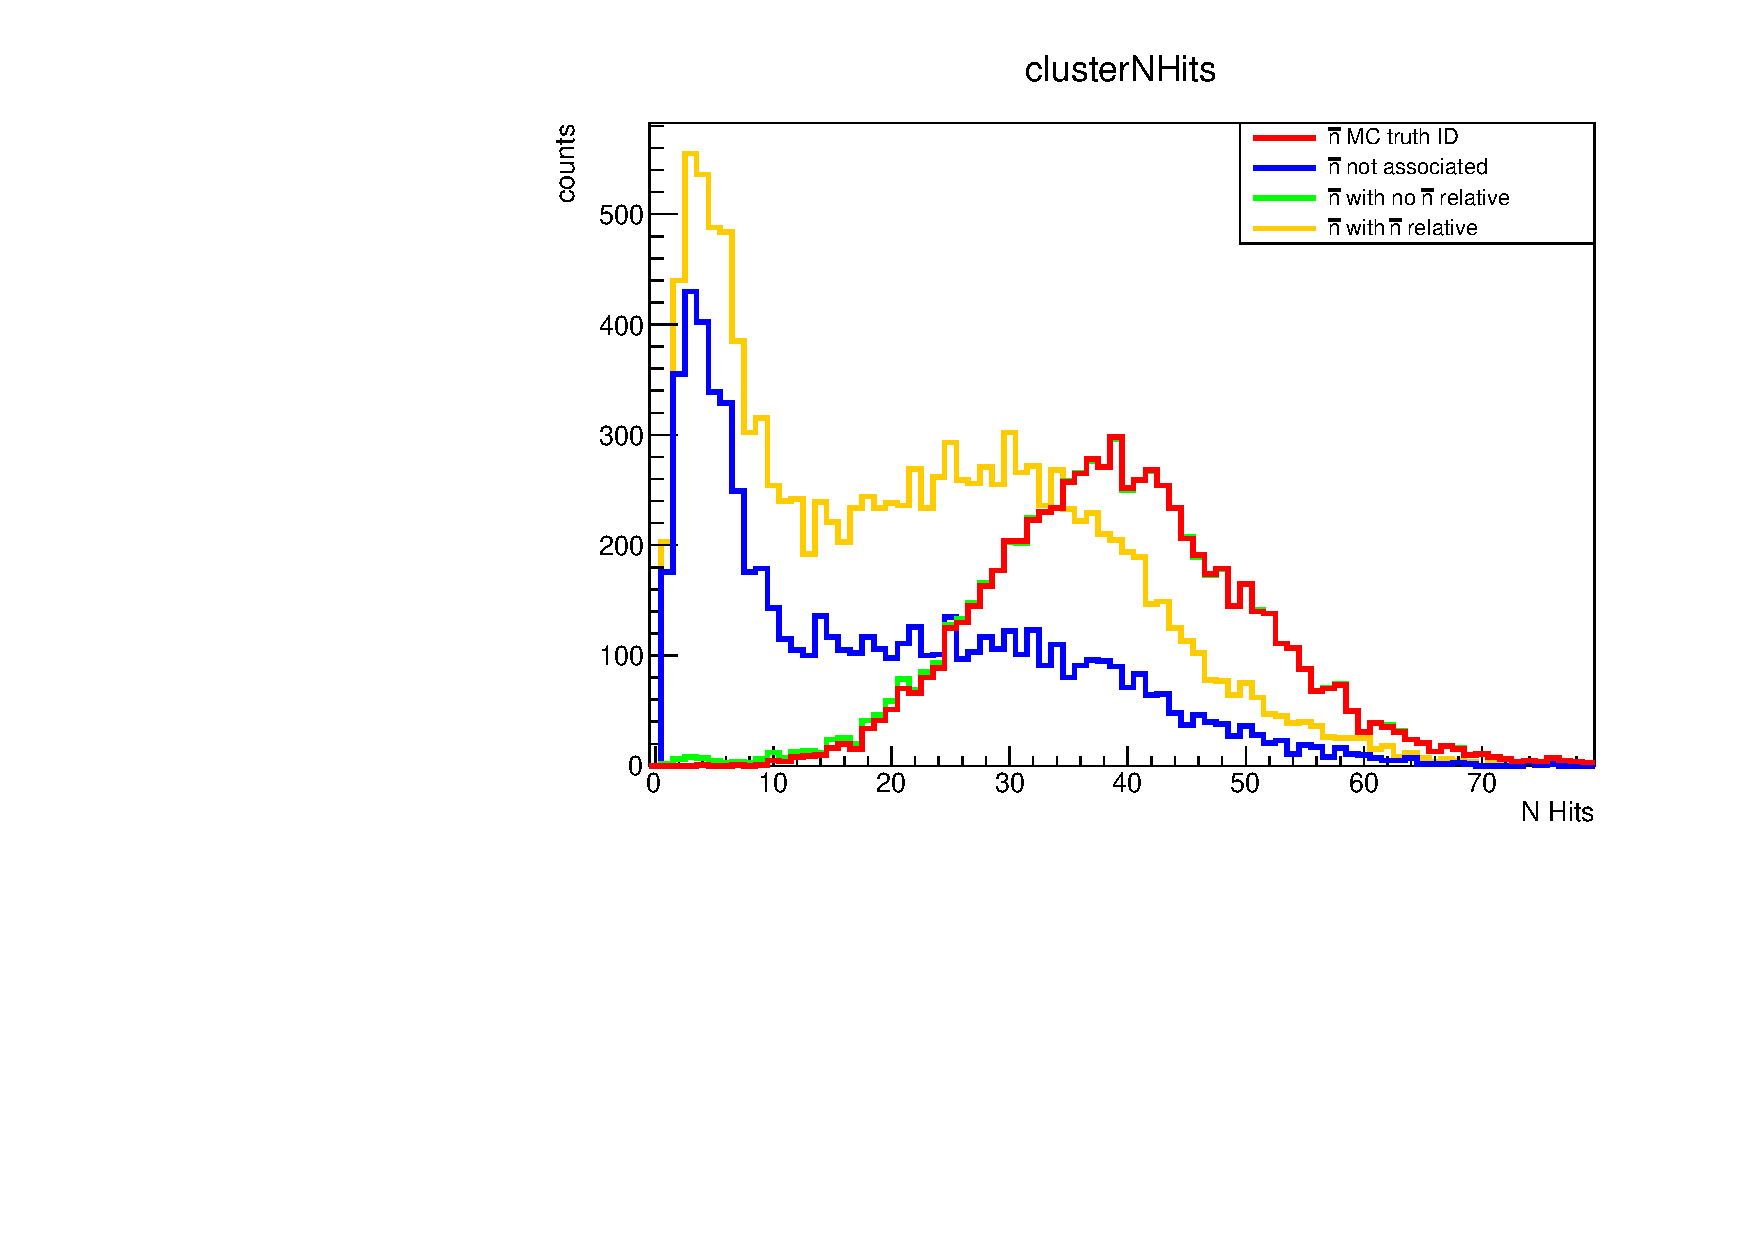
\includegraphics[width=0.49\textwidth]{nbar_MC/images/clusterNHits_isr_ancestor.pdf}
   
     \caption{Comparison of reconstructed cluster variables for $\bar{n}$ candidates with different ancestor selection (ISR case)}
     \label{fig:cluster_ISR}
\end{figure}

\newpage
The obtained cluster variables in NO ISR case are shown below:
 \begin{figure}[H]
    \centering
    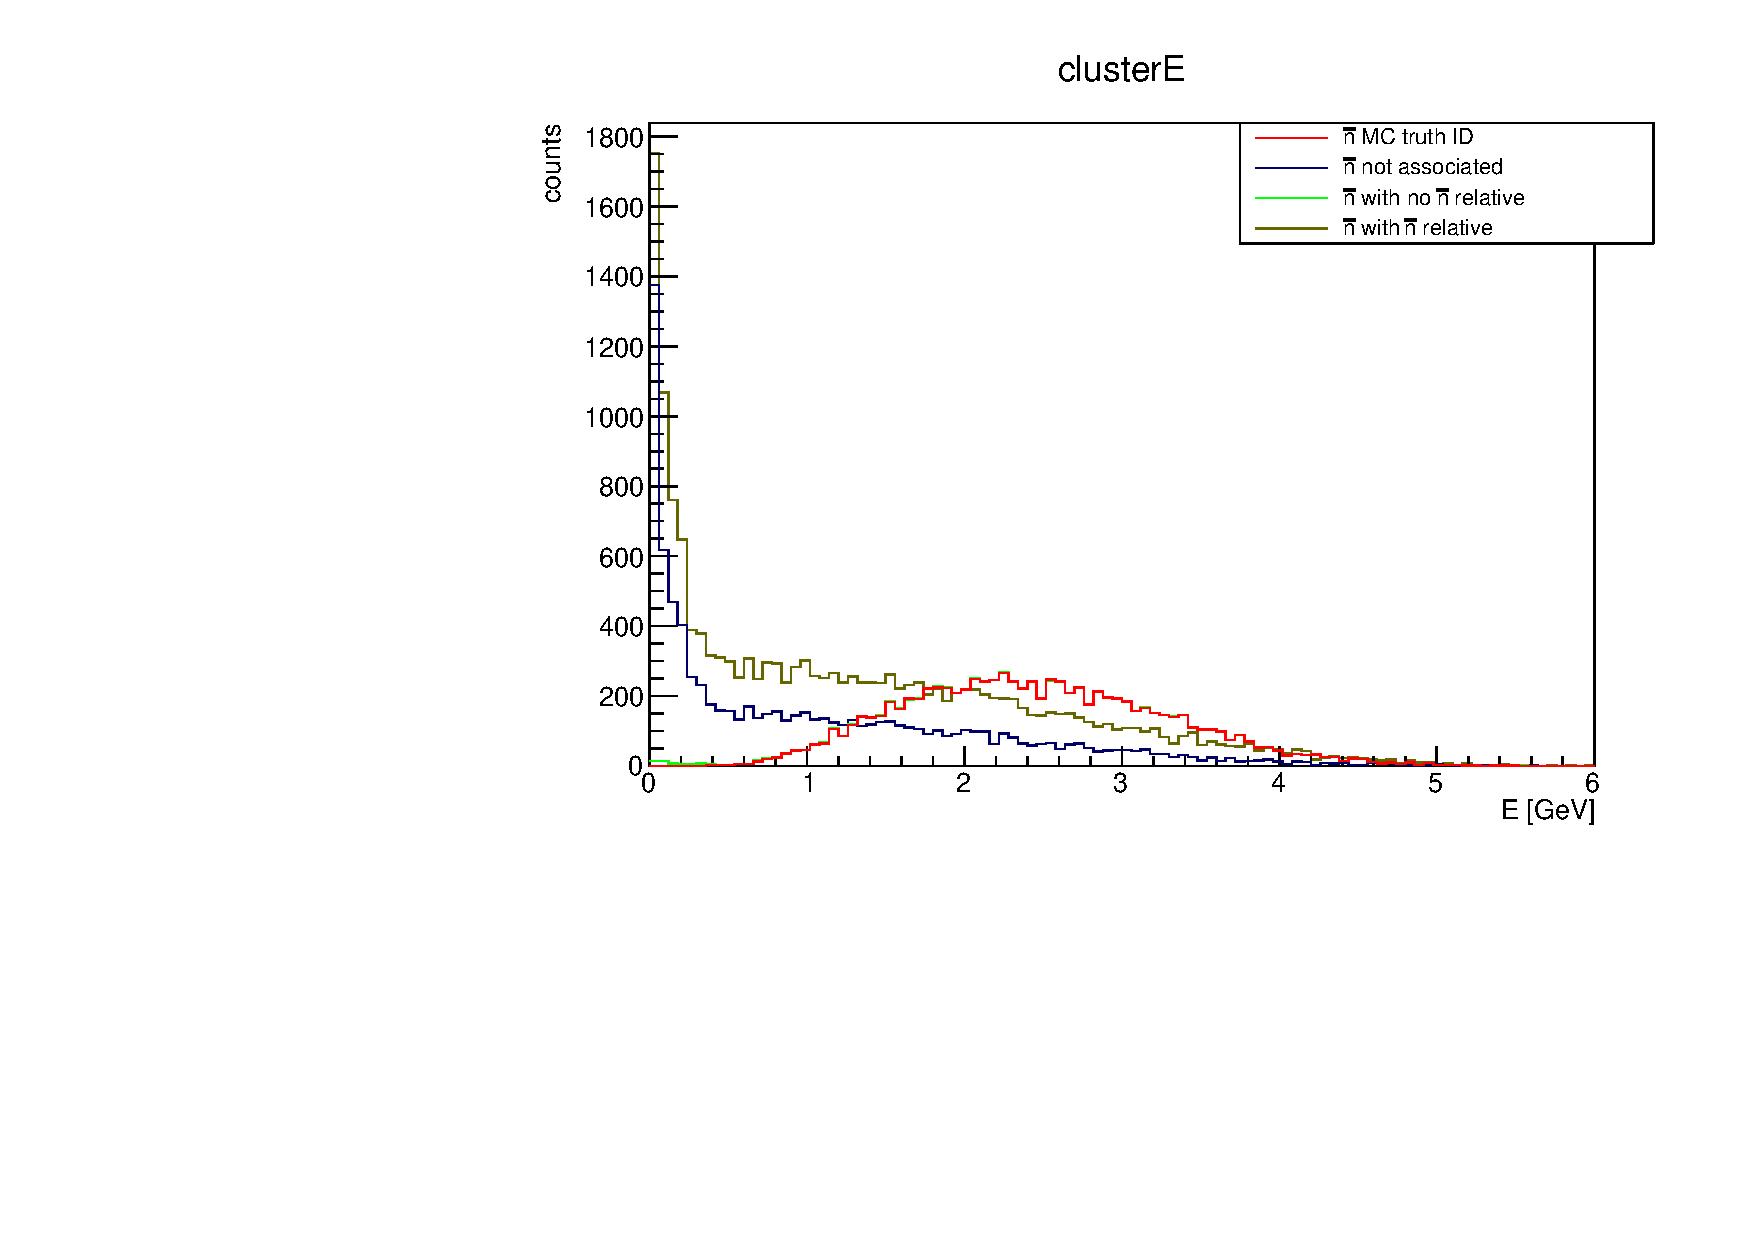
\includegraphics[width=0.49\textwidth]{nbar_MC/images/clusterE_nog_ancestor.pdf}
    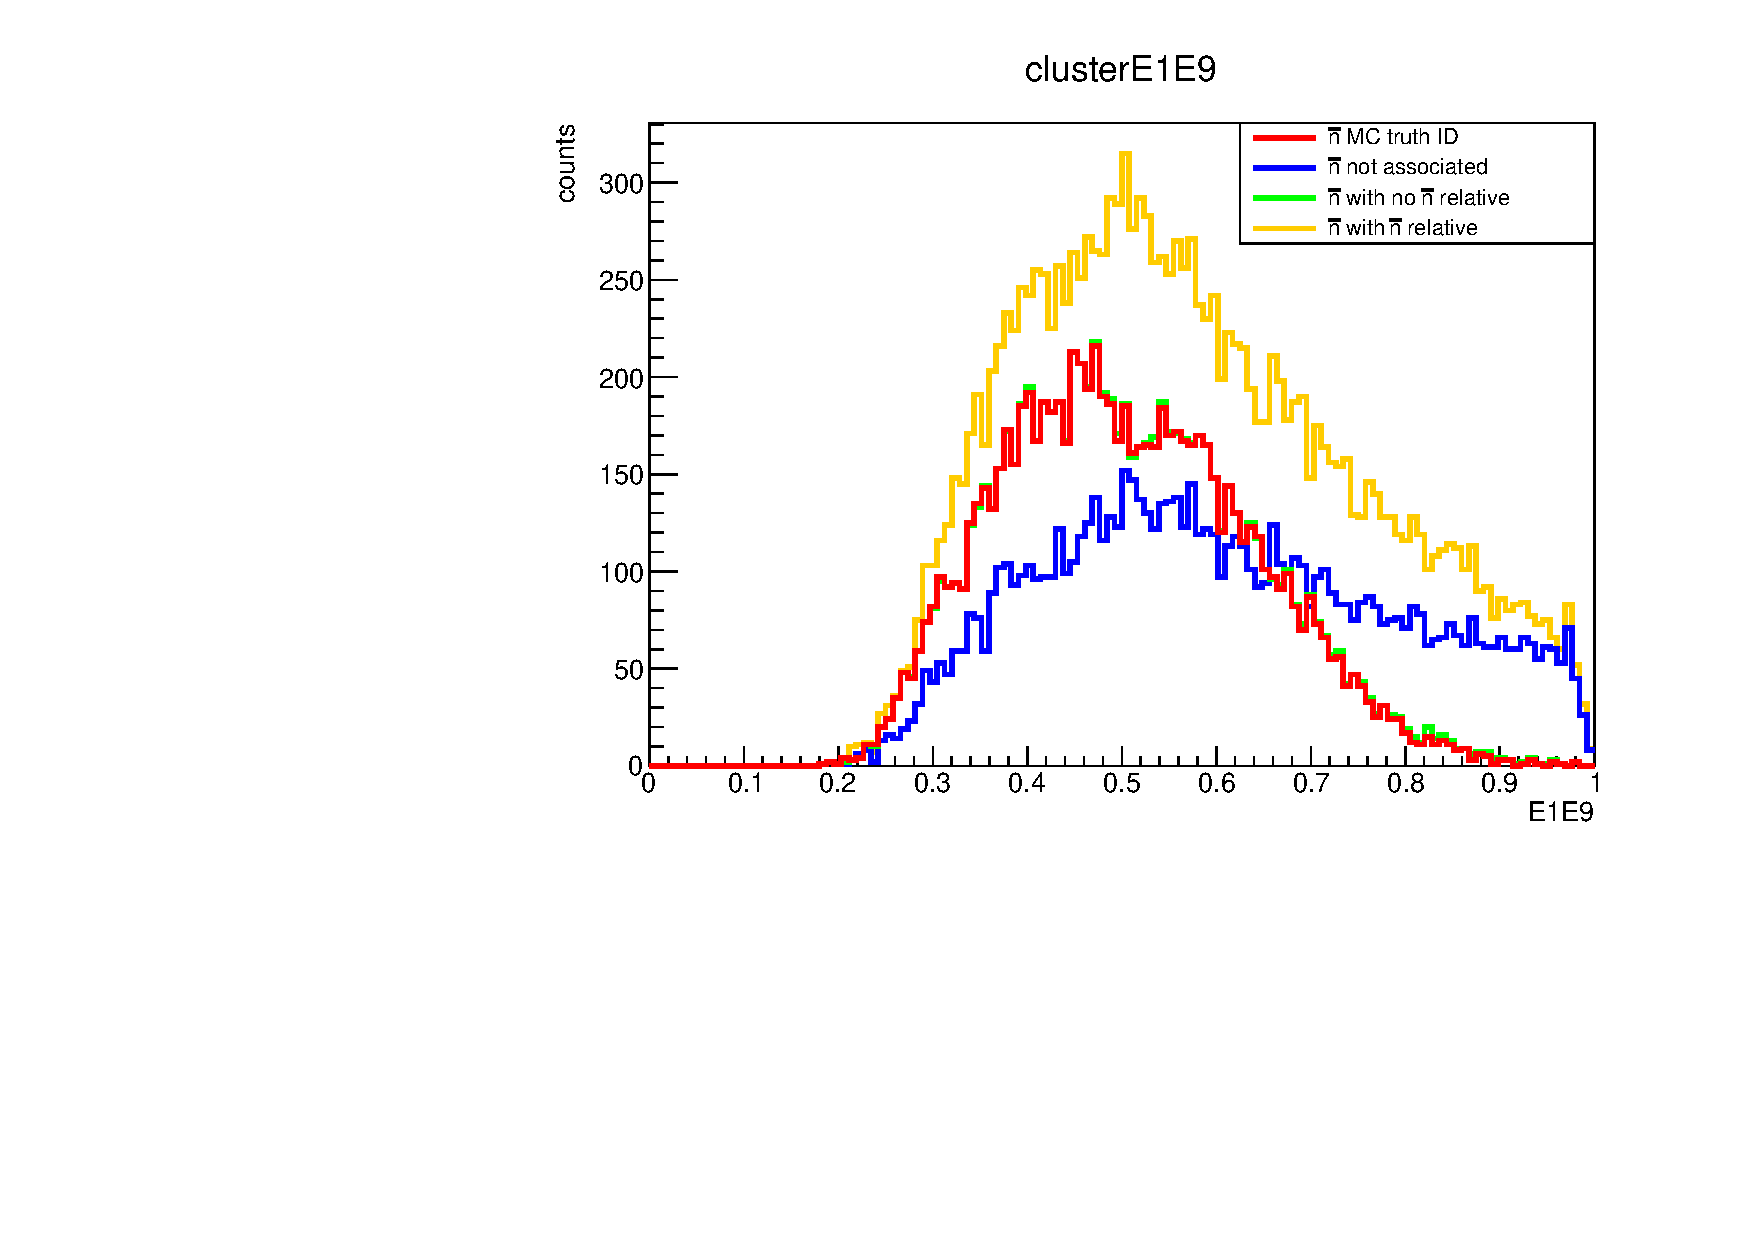
\includegraphics[width=0.49\textwidth]{nbar_MC/images/clusterE1E9_nog_ancestor.pdf}
    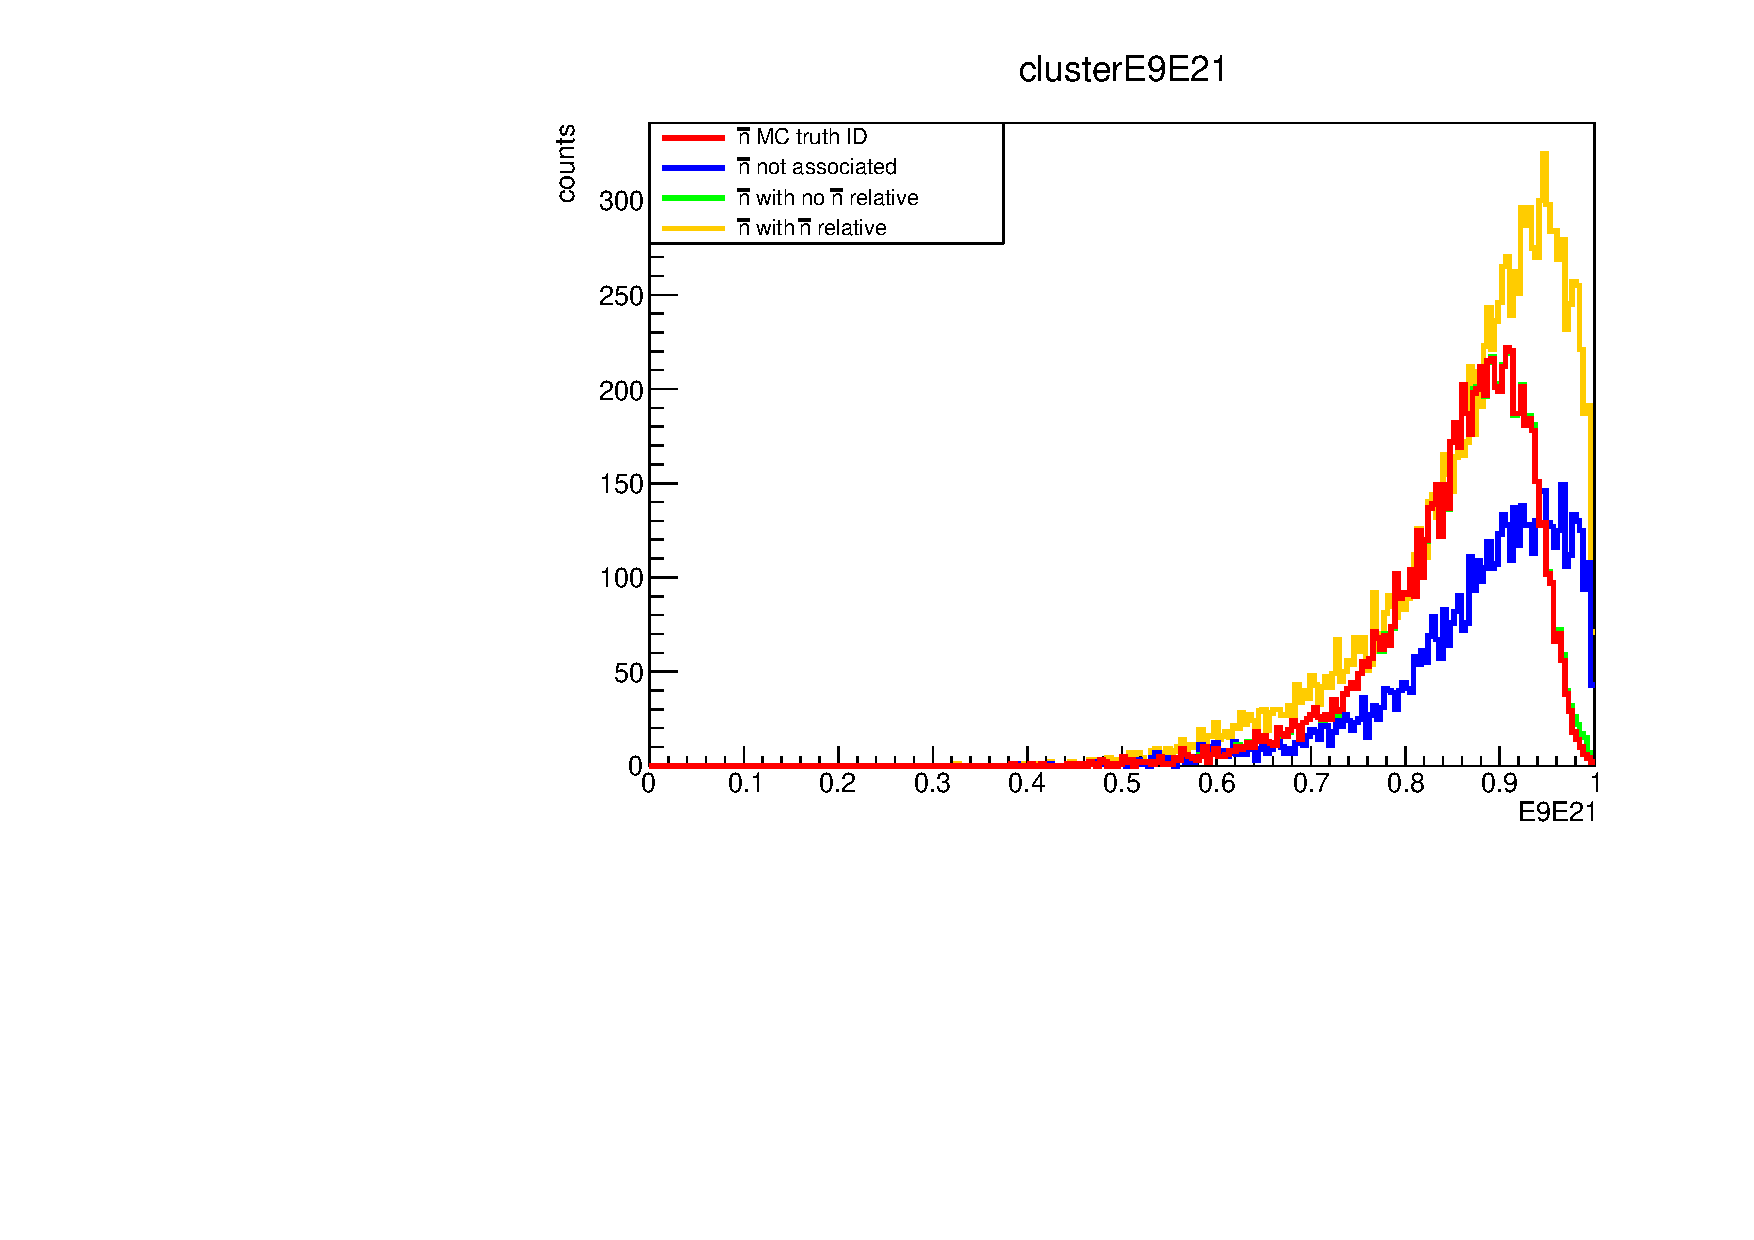
\includegraphics[width=0.49\textwidth]{nbar_MC/images/clusterE9E21_nog_ancestor.pdf}
    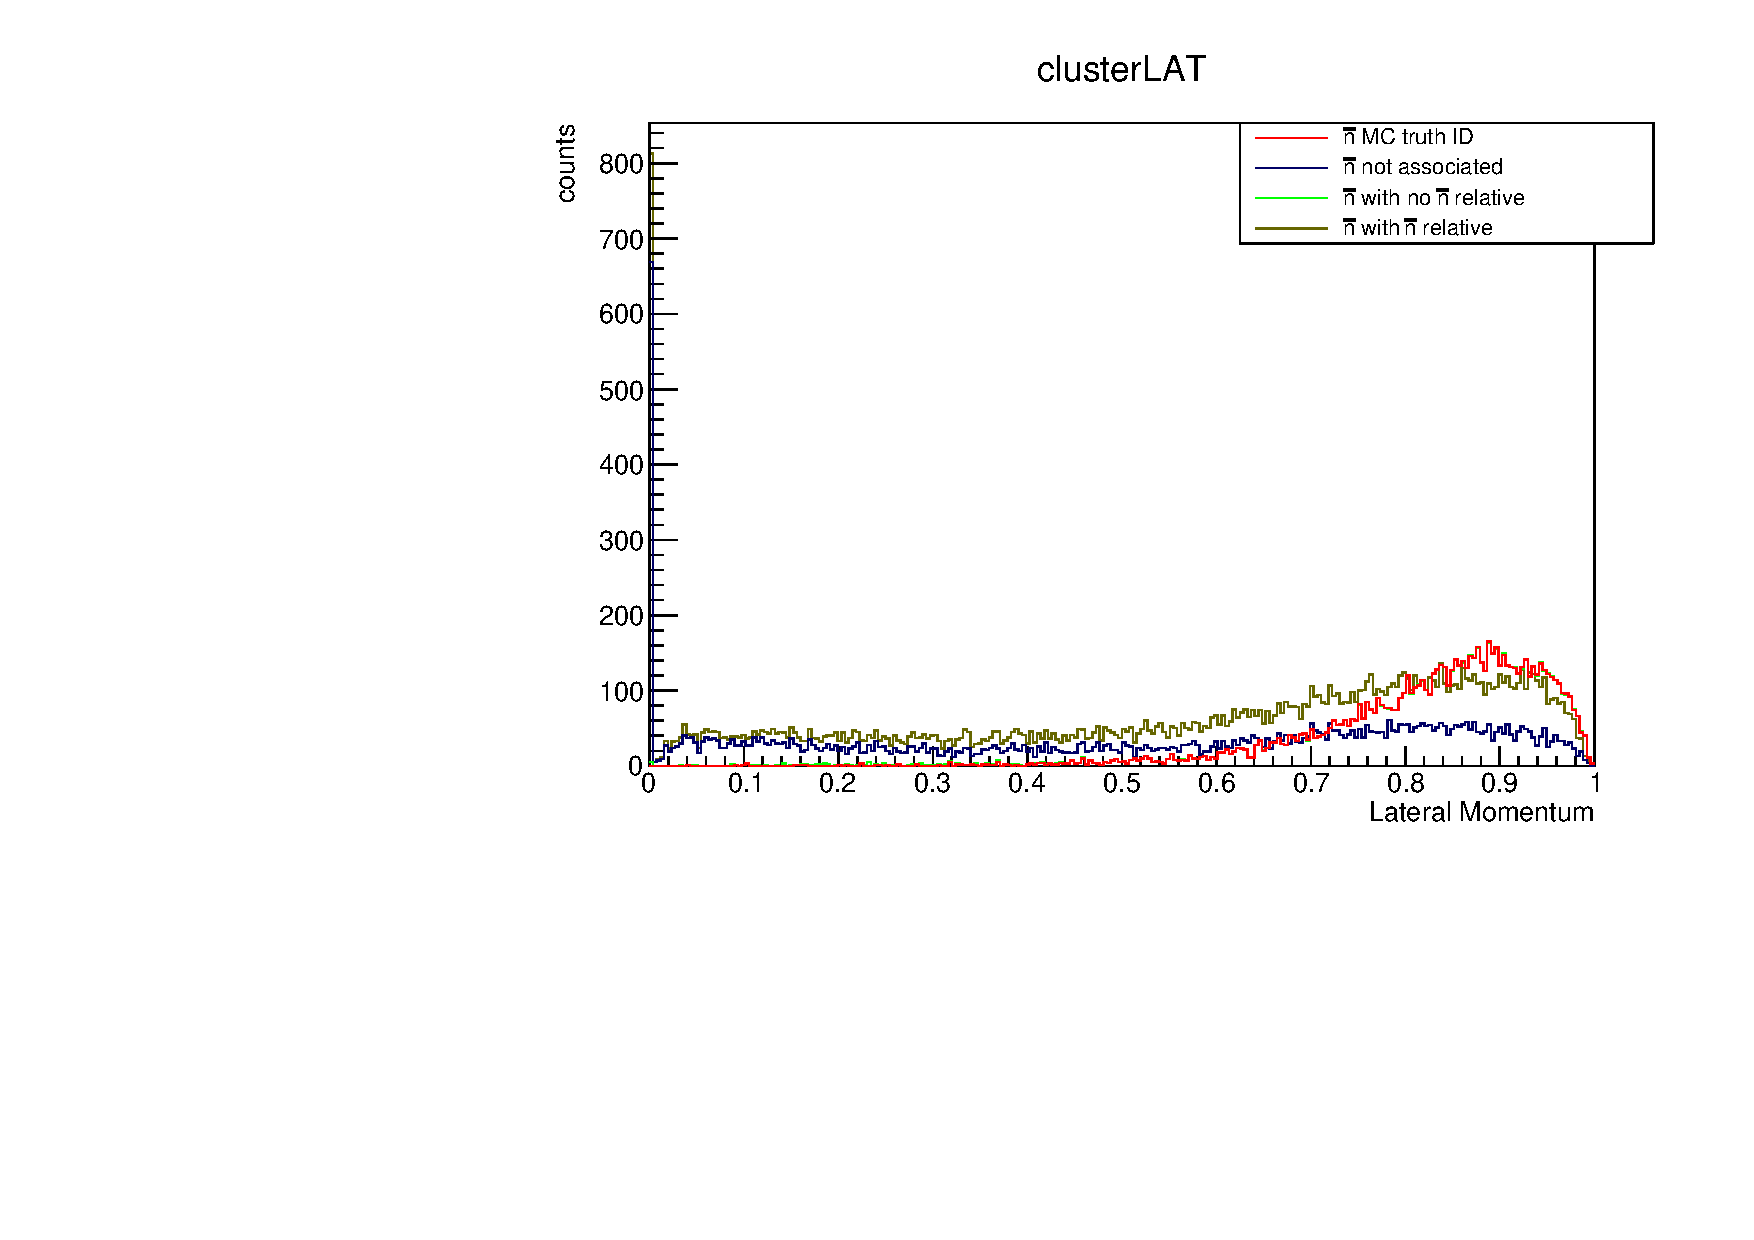
\includegraphics[width=0.49\textwidth]{nbar_MC/images/clusterLAT_nog_ancestor.pdf}
    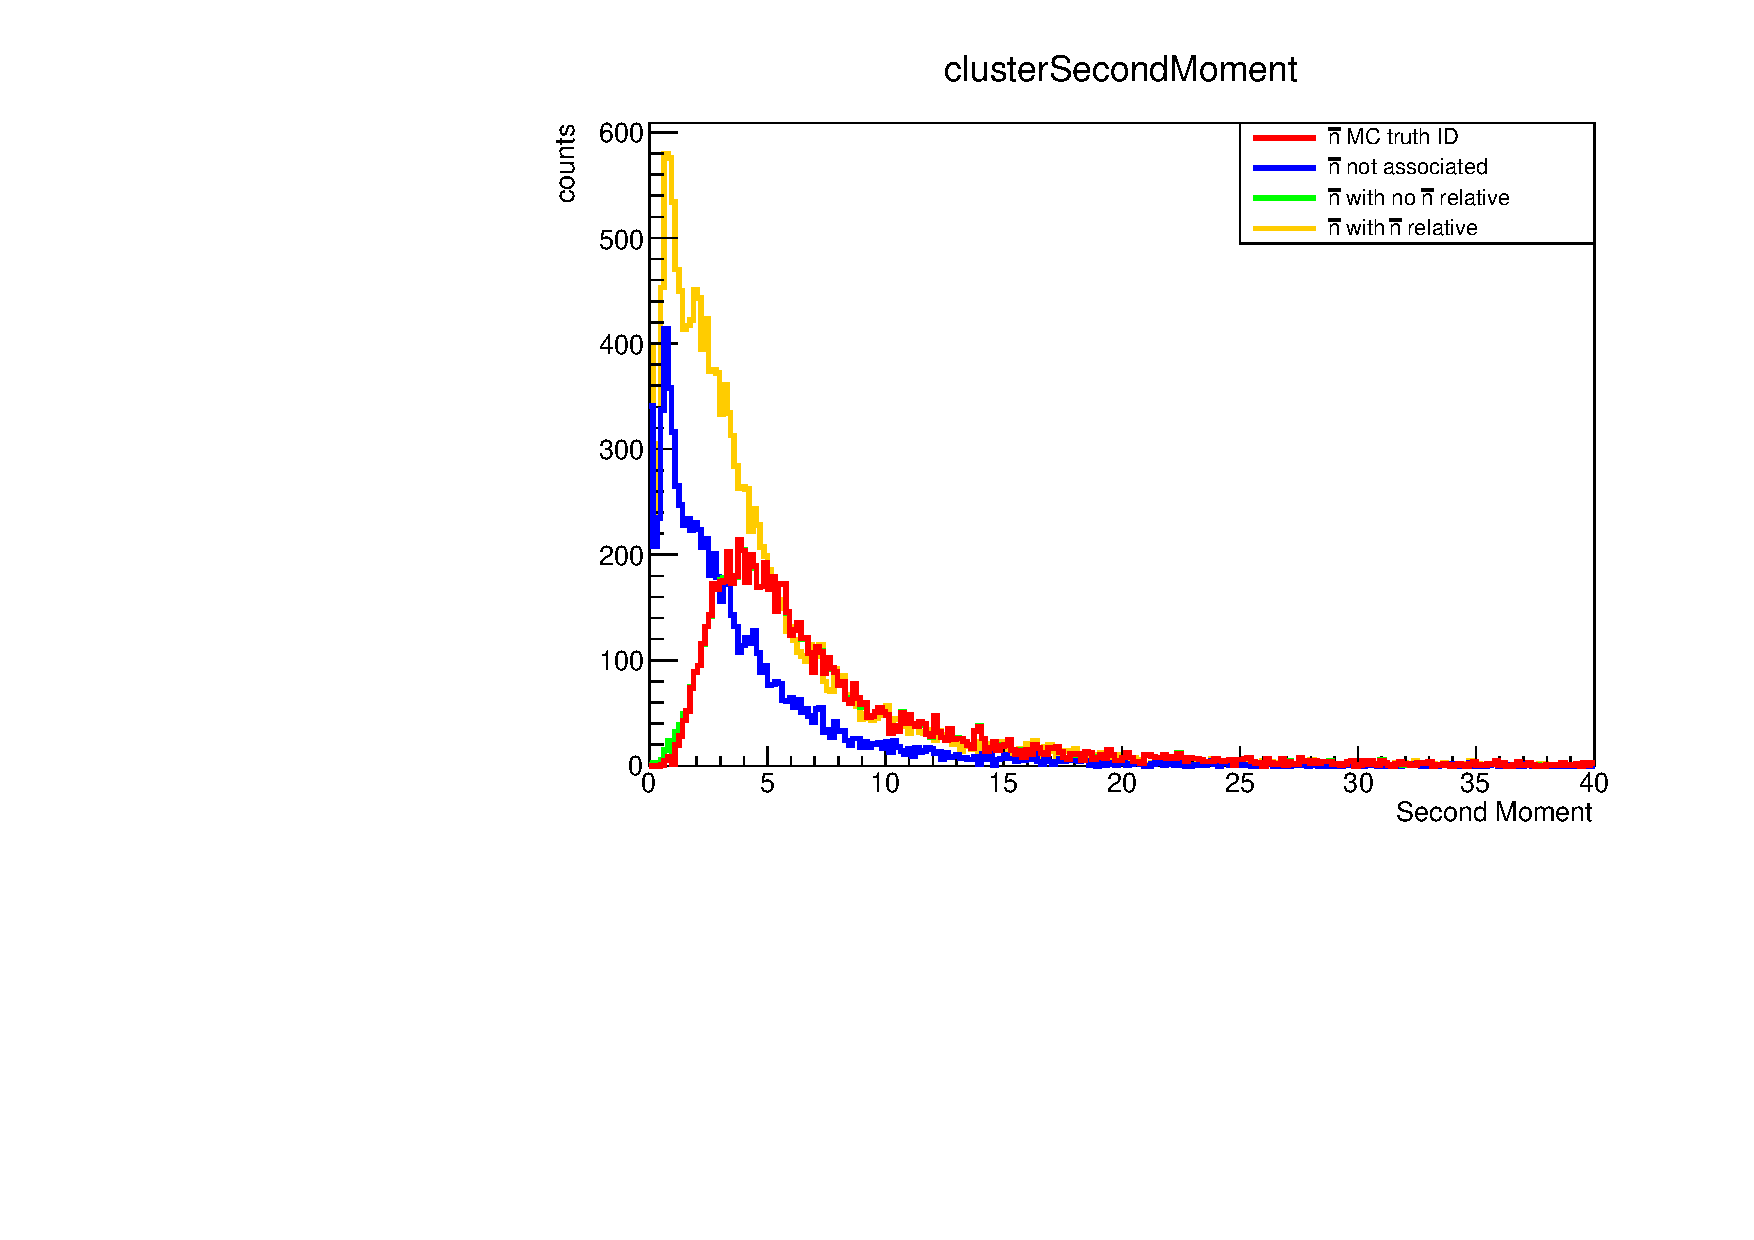
\includegraphics[width=0.49\textwidth]{nbar_MC/images/clusterSecondMoment_nog_ancestor.pdf}
    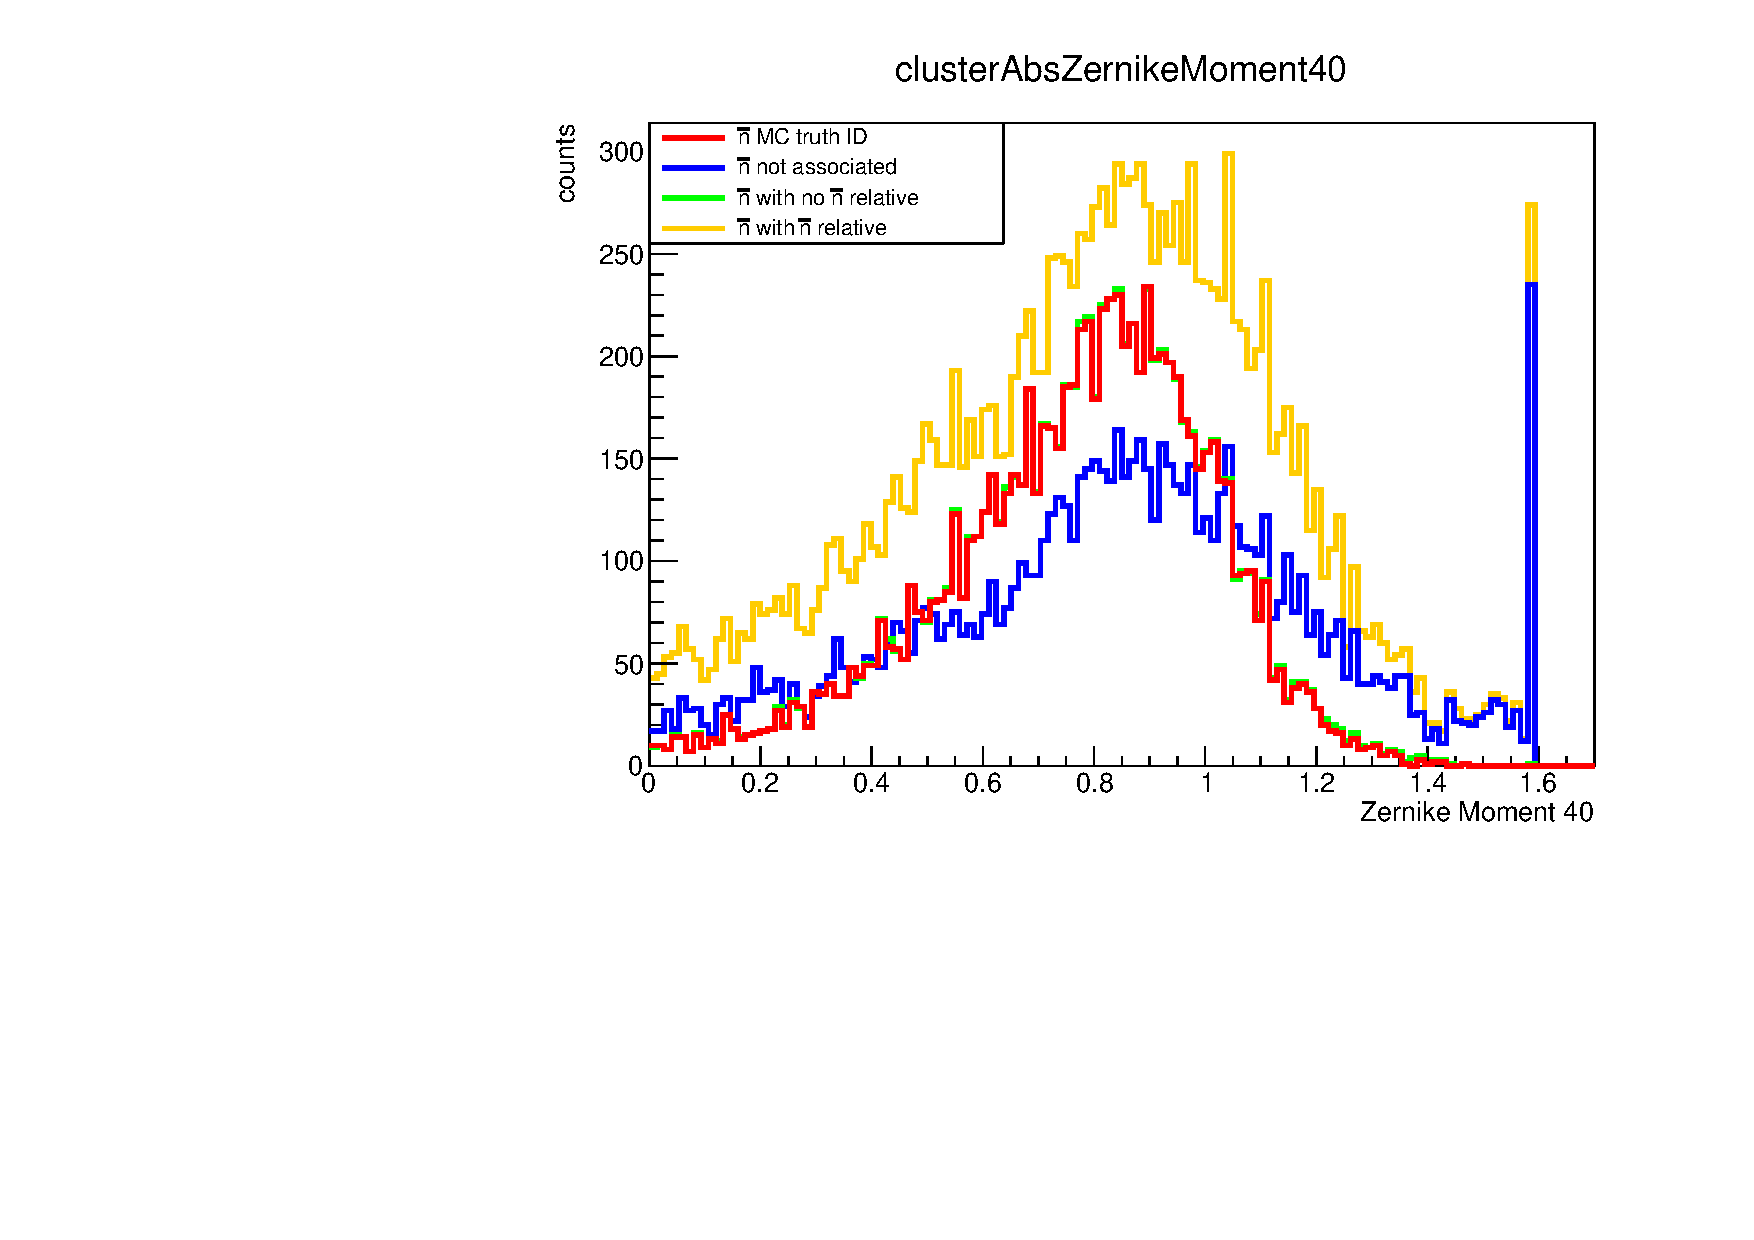
\includegraphics[width=0.49\textwidth]{nbar_MC/images/clusterAbsZernikeMoment40_nog_ancestor.pdf}
    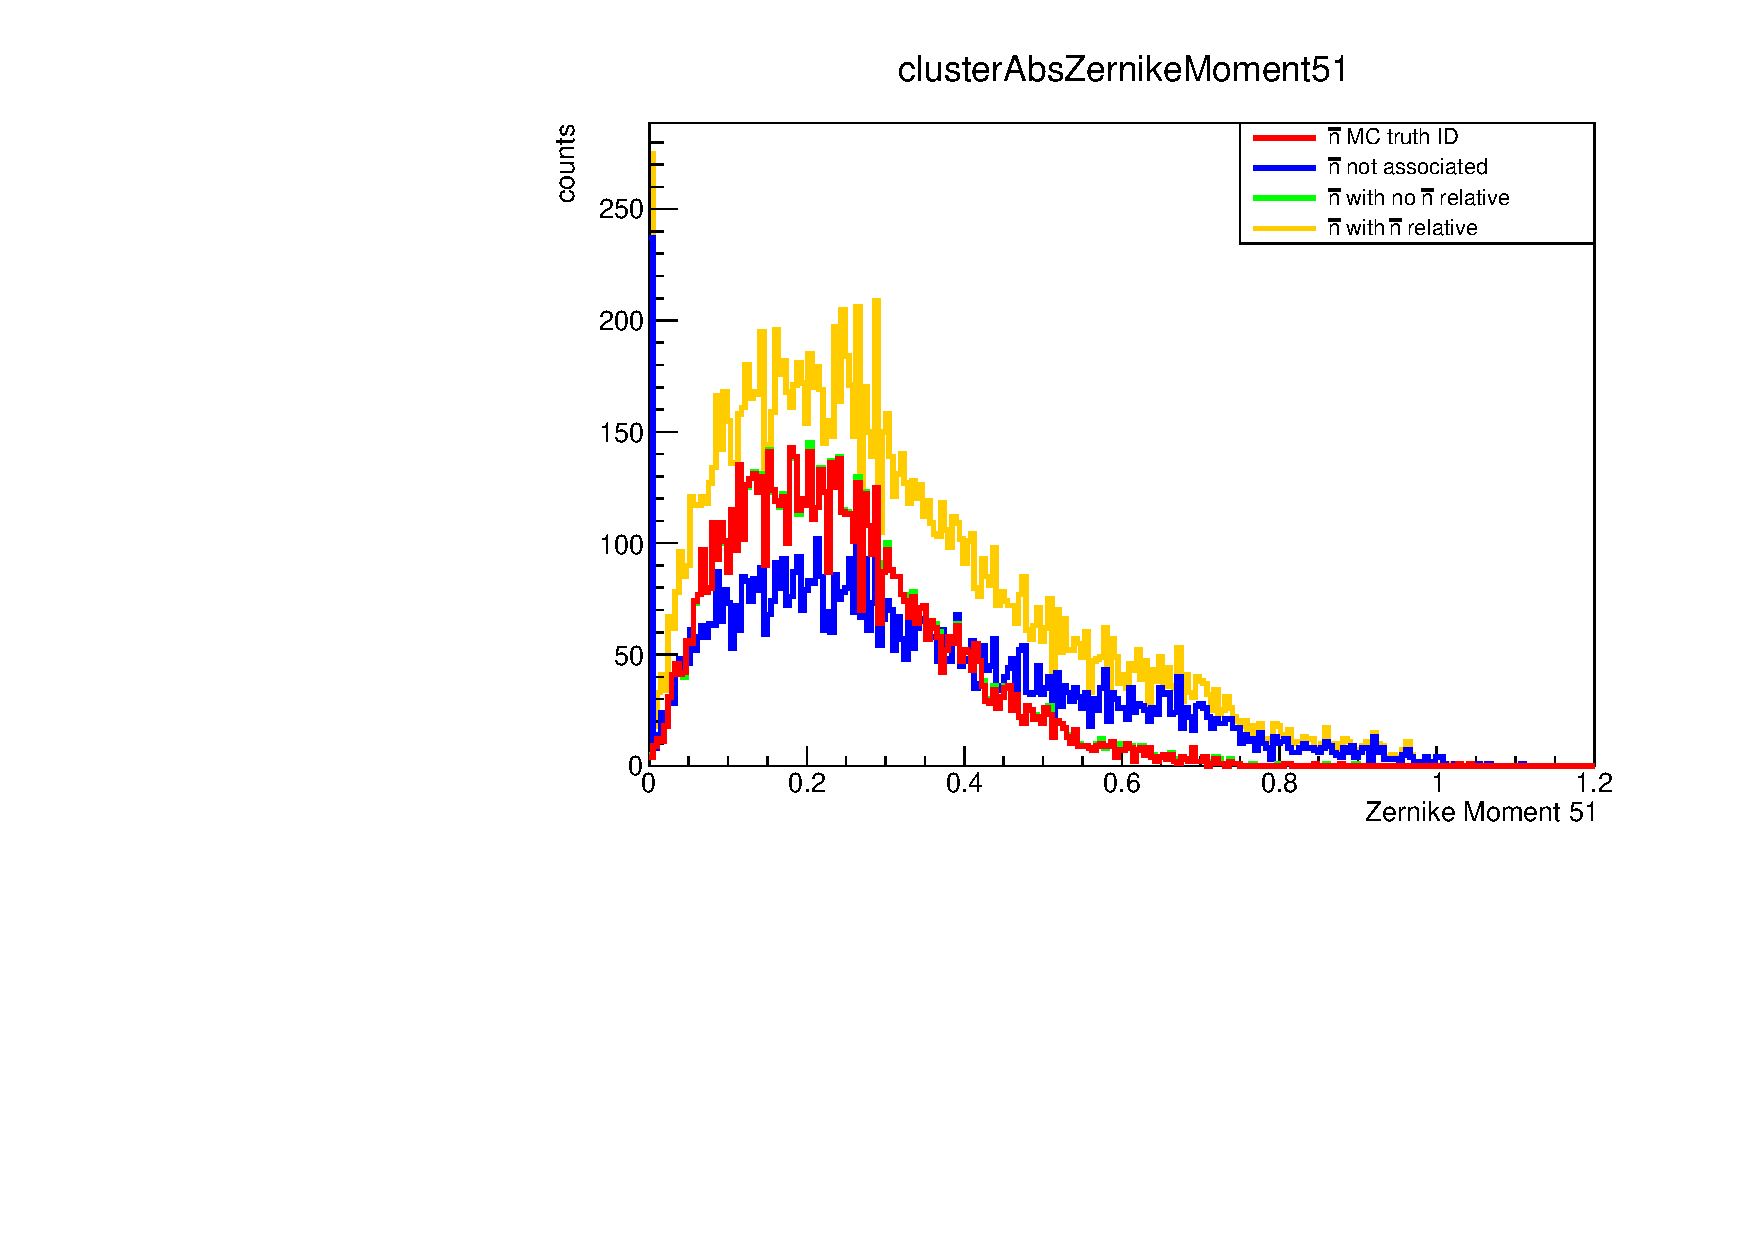
\includegraphics[width=0.49\textwidth]{nbar_MC/images/clusterAbsZernikeMoment51_nog_ancestor.pdf}
    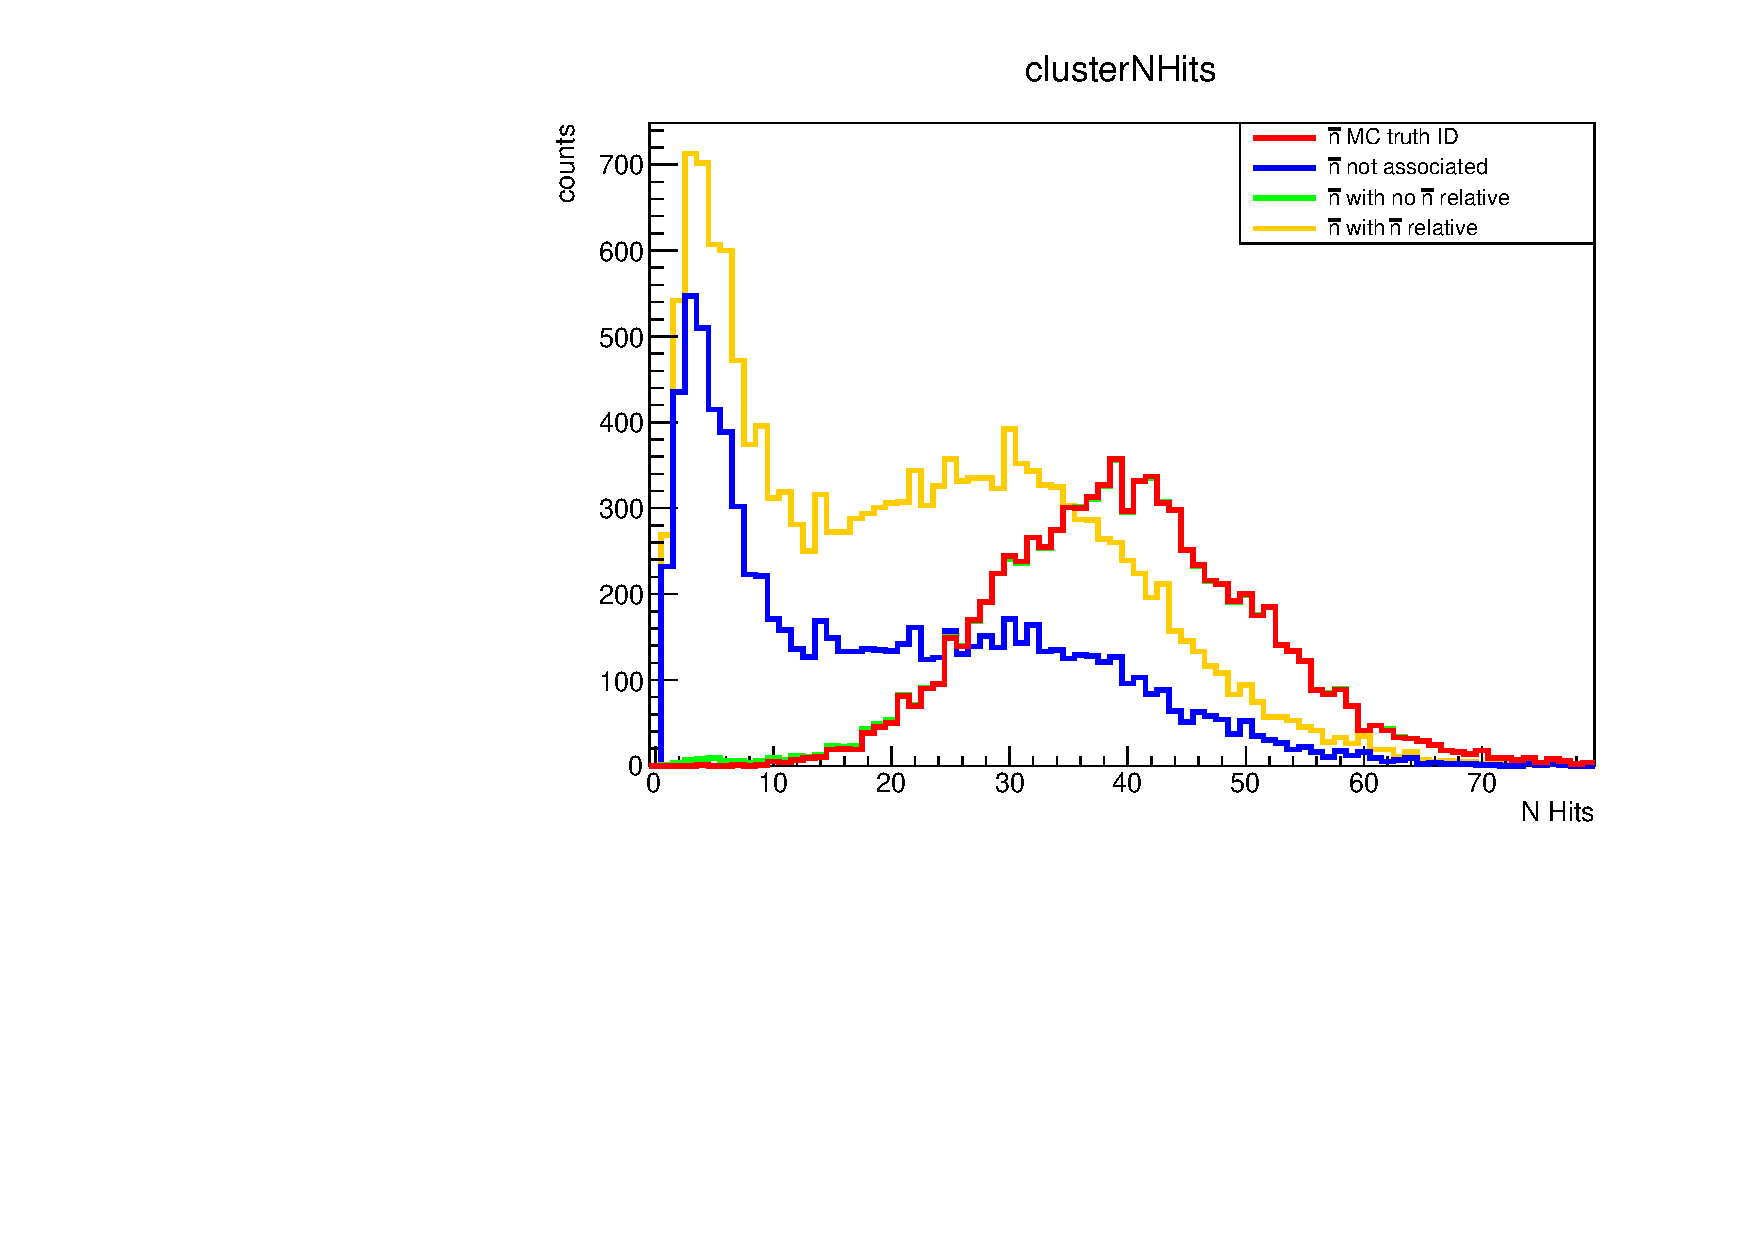
\includegraphics[width=0.49\textwidth]{nbar_MC/images/clusterNHits_nog_ancestor.pdf}
   
     \caption{Comparison of reconstructed cluster variables for $\bar{n}$ candidates with different ancestor selection (NO ISR case)}
     \label{fig:cluster_NOISR}

\end{figure}


\newpage
The obtained cluster variables in ISR case are shown below:
 \begin{figure}[H]
    \centering
    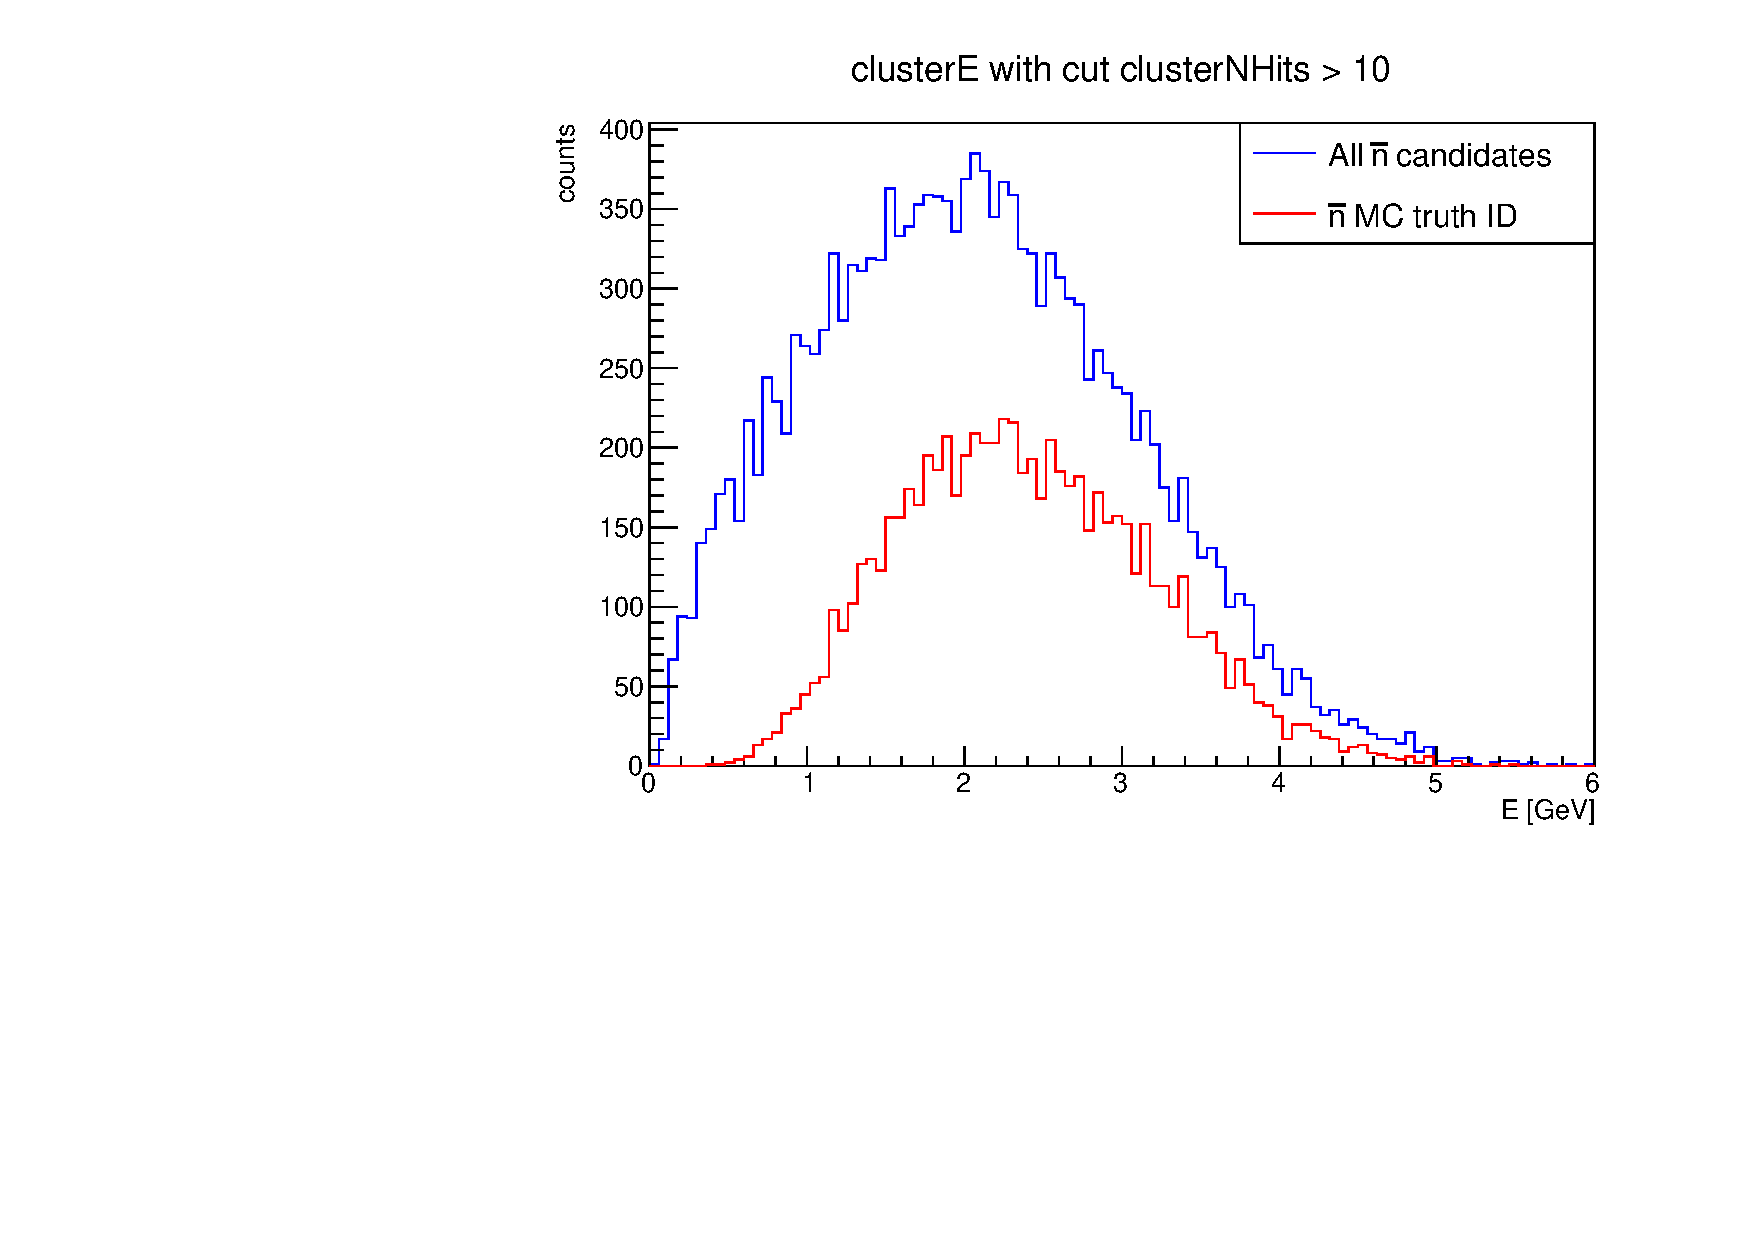
\includegraphics[width=0.49\textwidth]{nbar_MC/images/clusterE_hitscut_isr.pdf}
    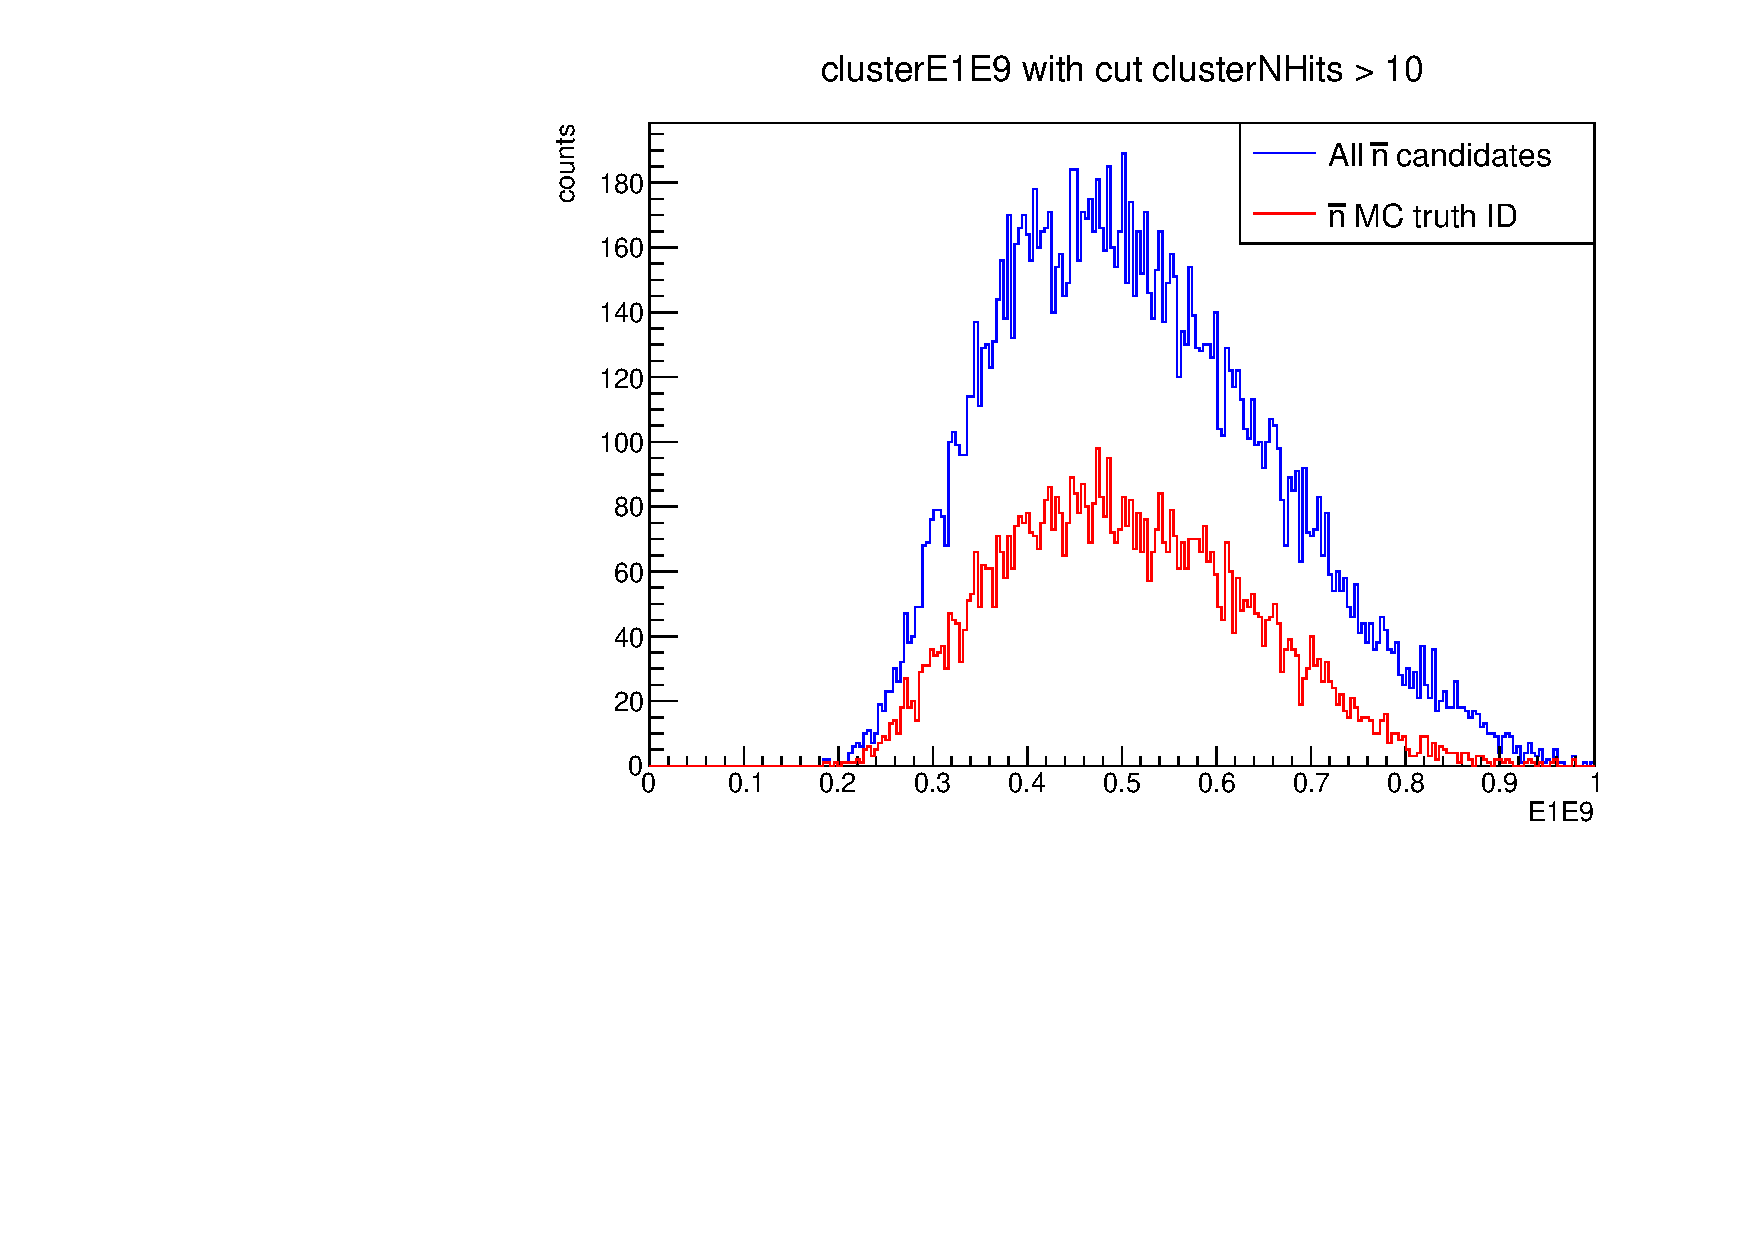
\includegraphics[width=0.49\textwidth]{nbar_MC/images/clusterE1E9_hitscut_isr.pdf}
    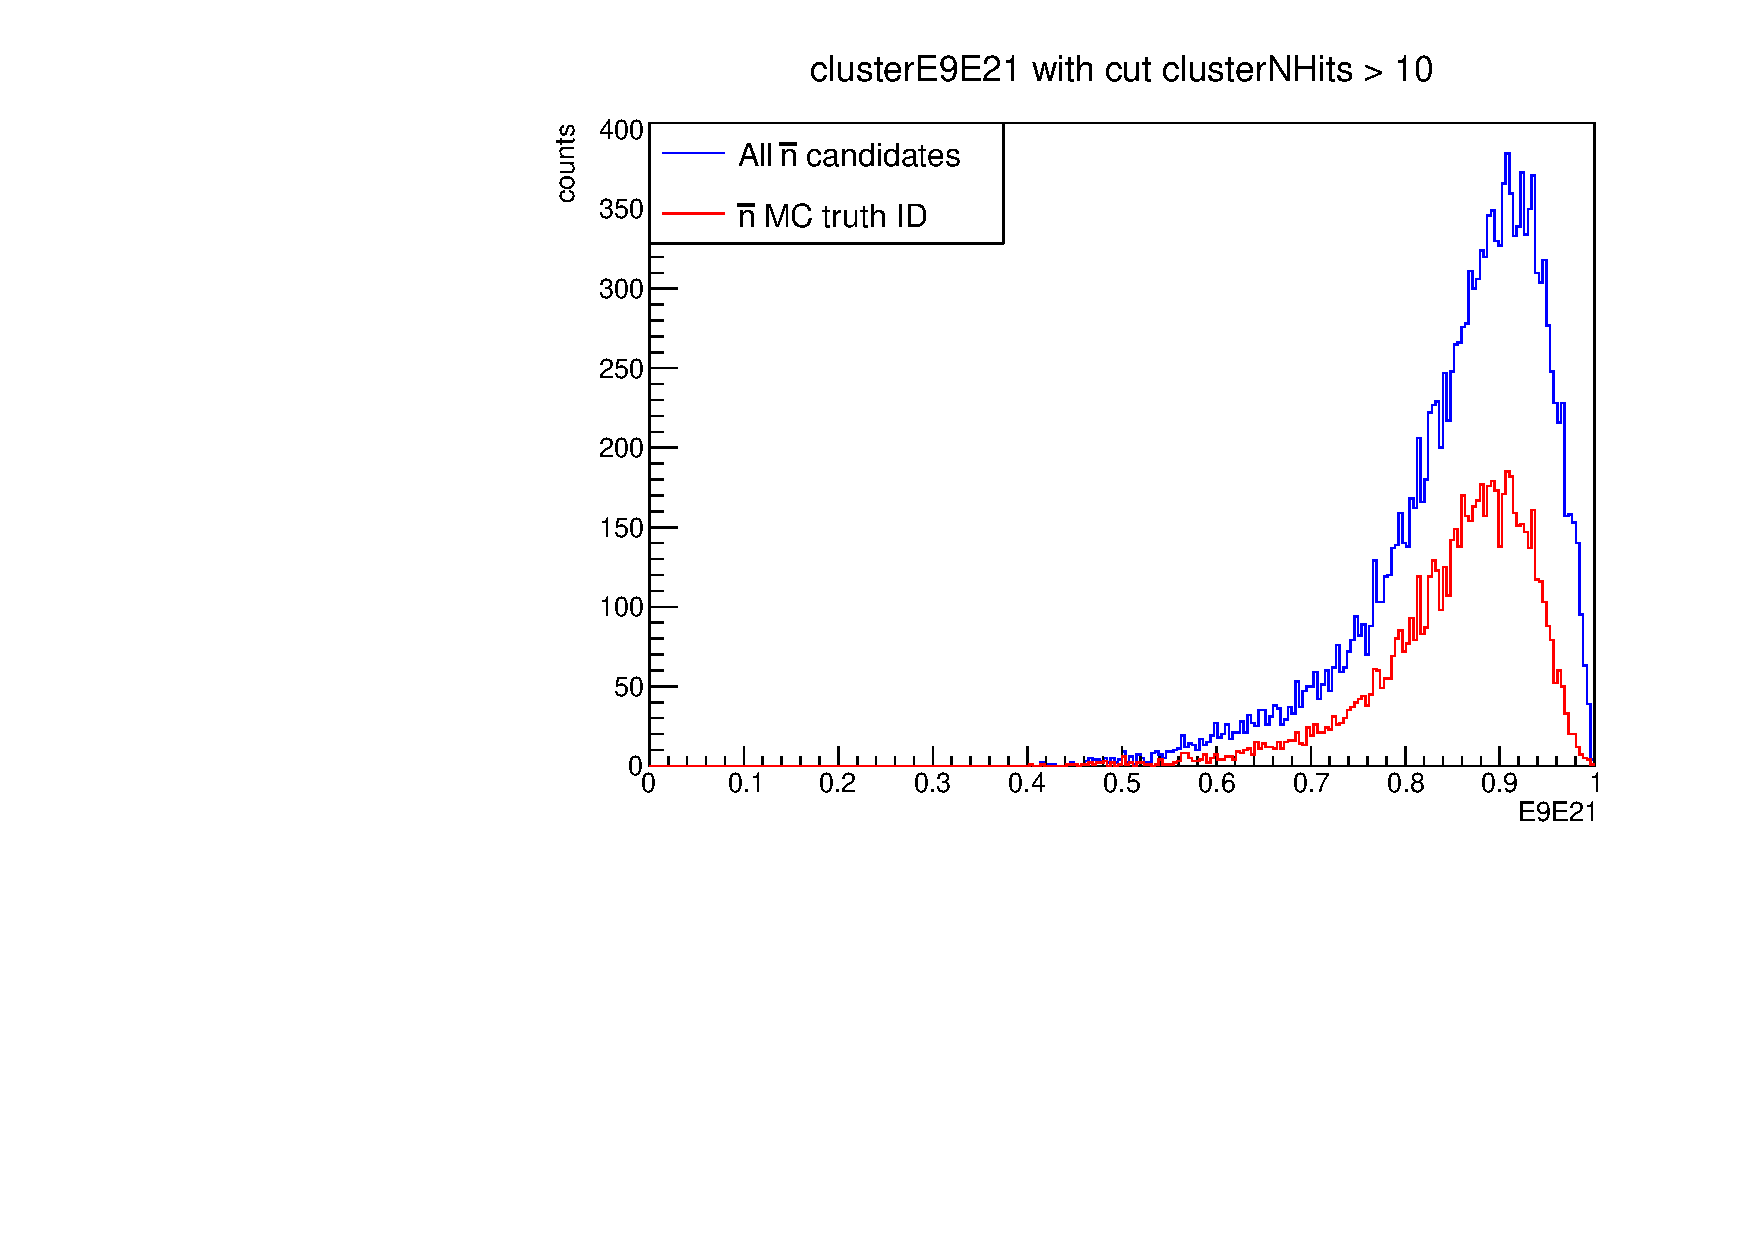
\includegraphics[width=0.49\textwidth]{nbar_MC/images/clusterE9E21_hitscut_isr.pdf}
    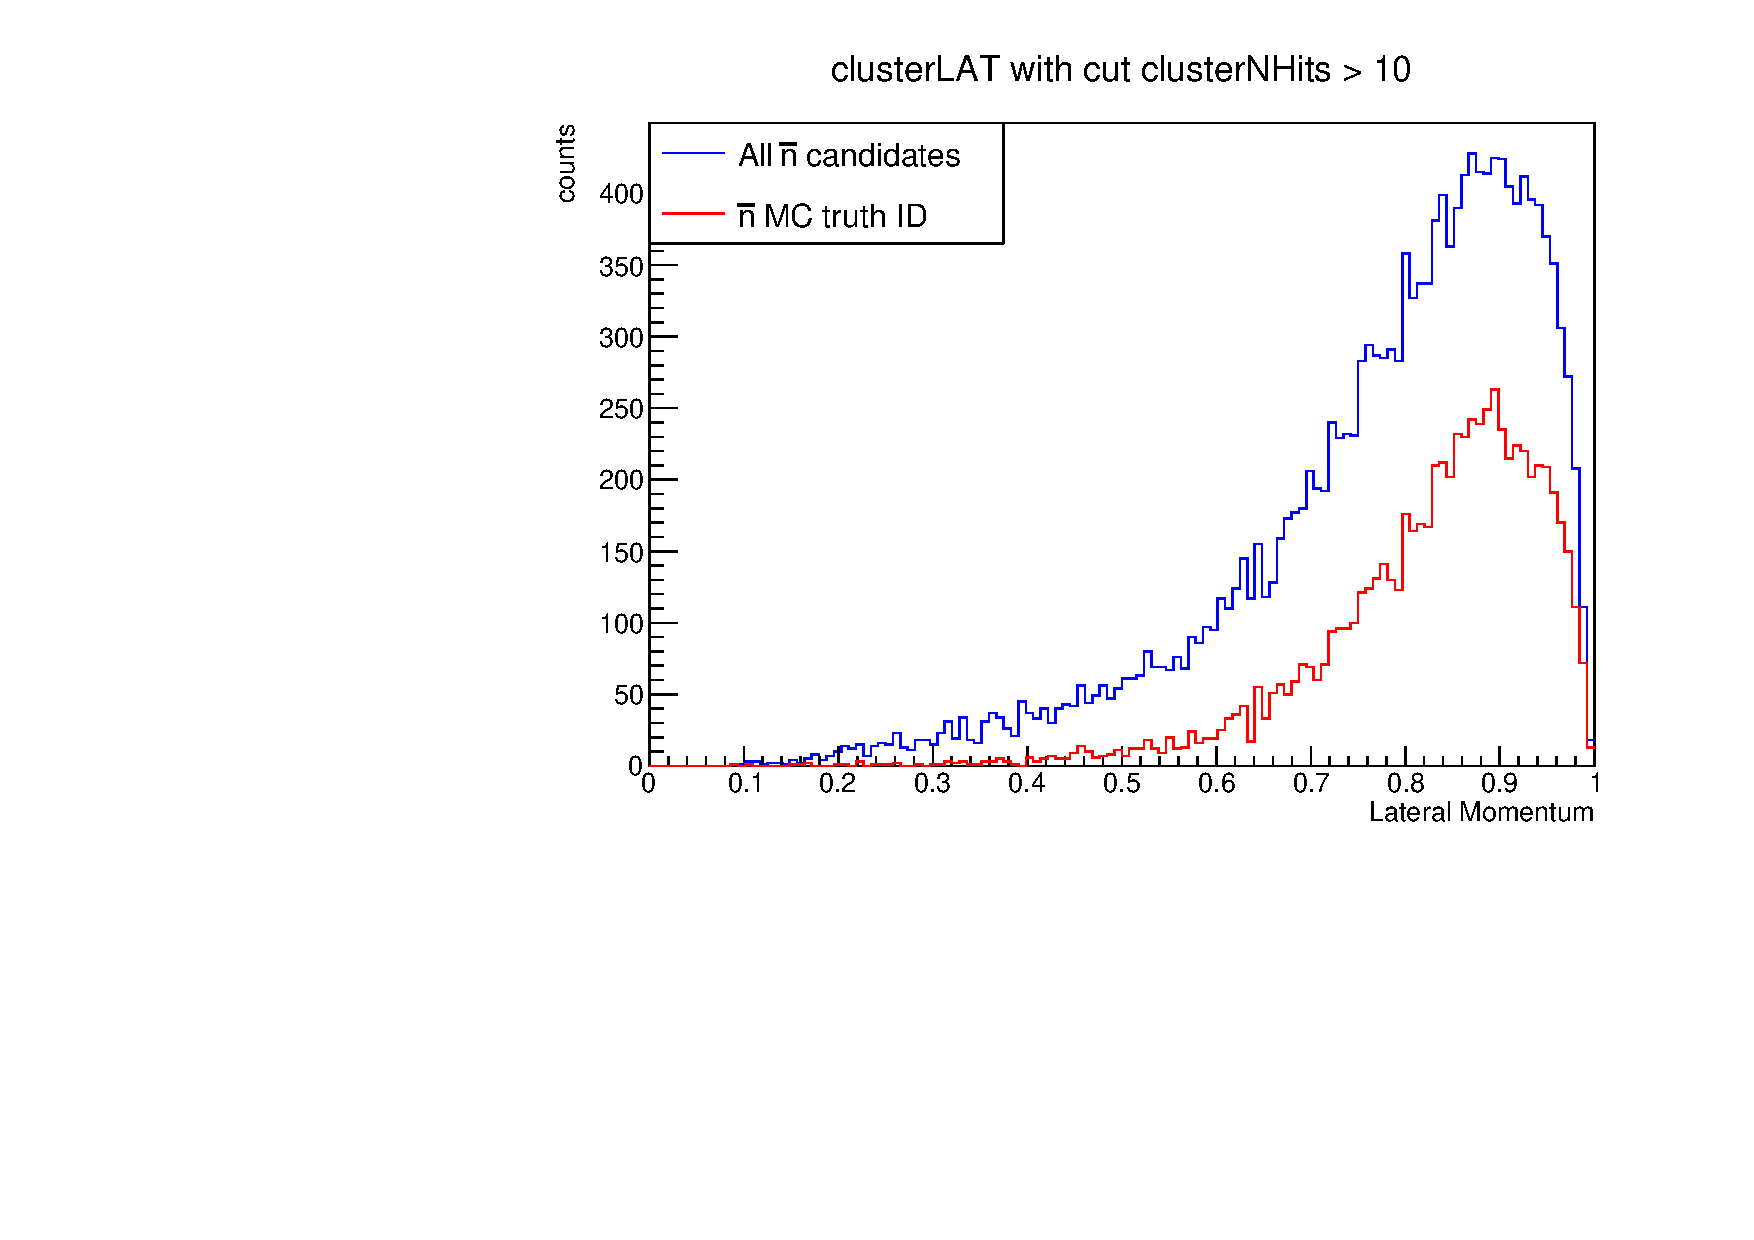
\includegraphics[width=0.49\textwidth]{nbar_MC/images/clusterLAT_hitscut_isr.pdf}
    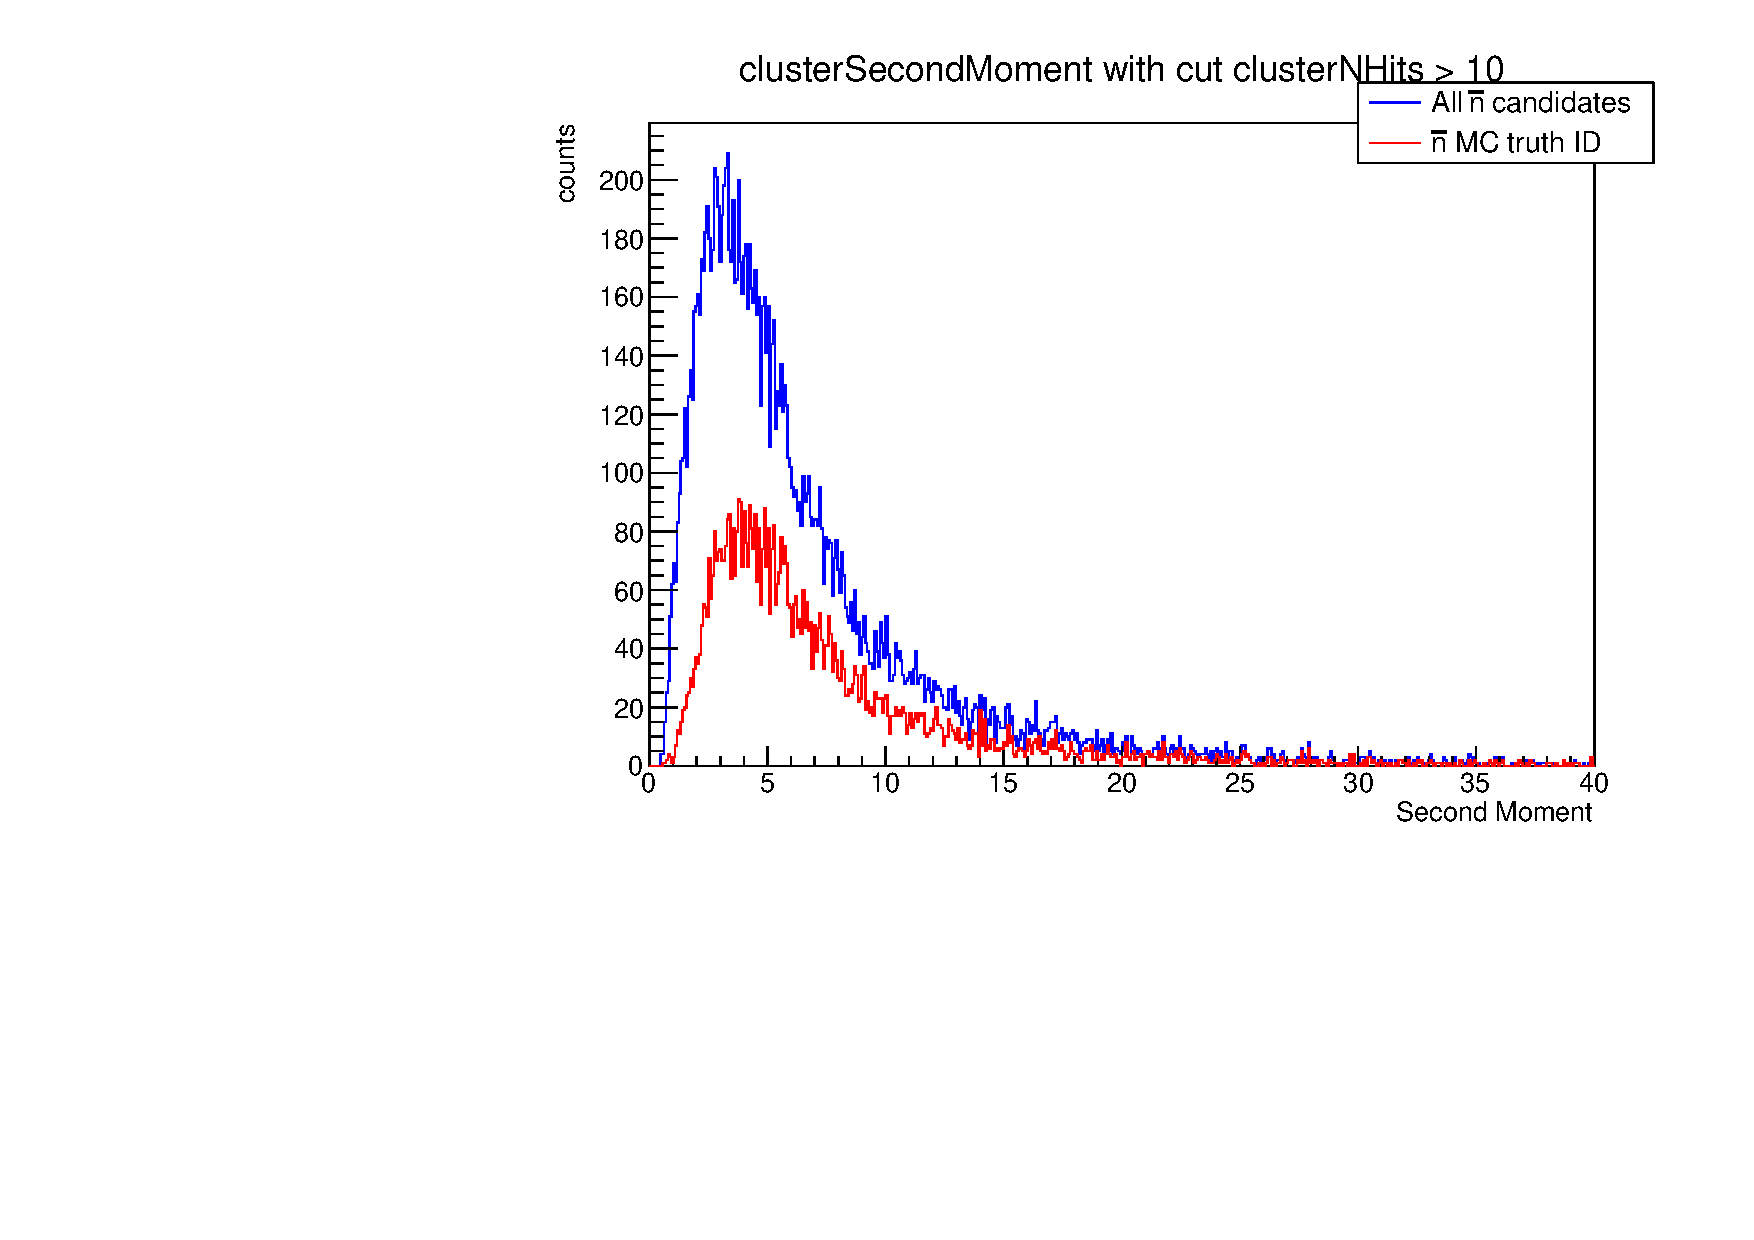
\includegraphics[width=0.49\textwidth]{nbar_MC/images/clusterSecondMoment_hitscut_isr.pdf}
    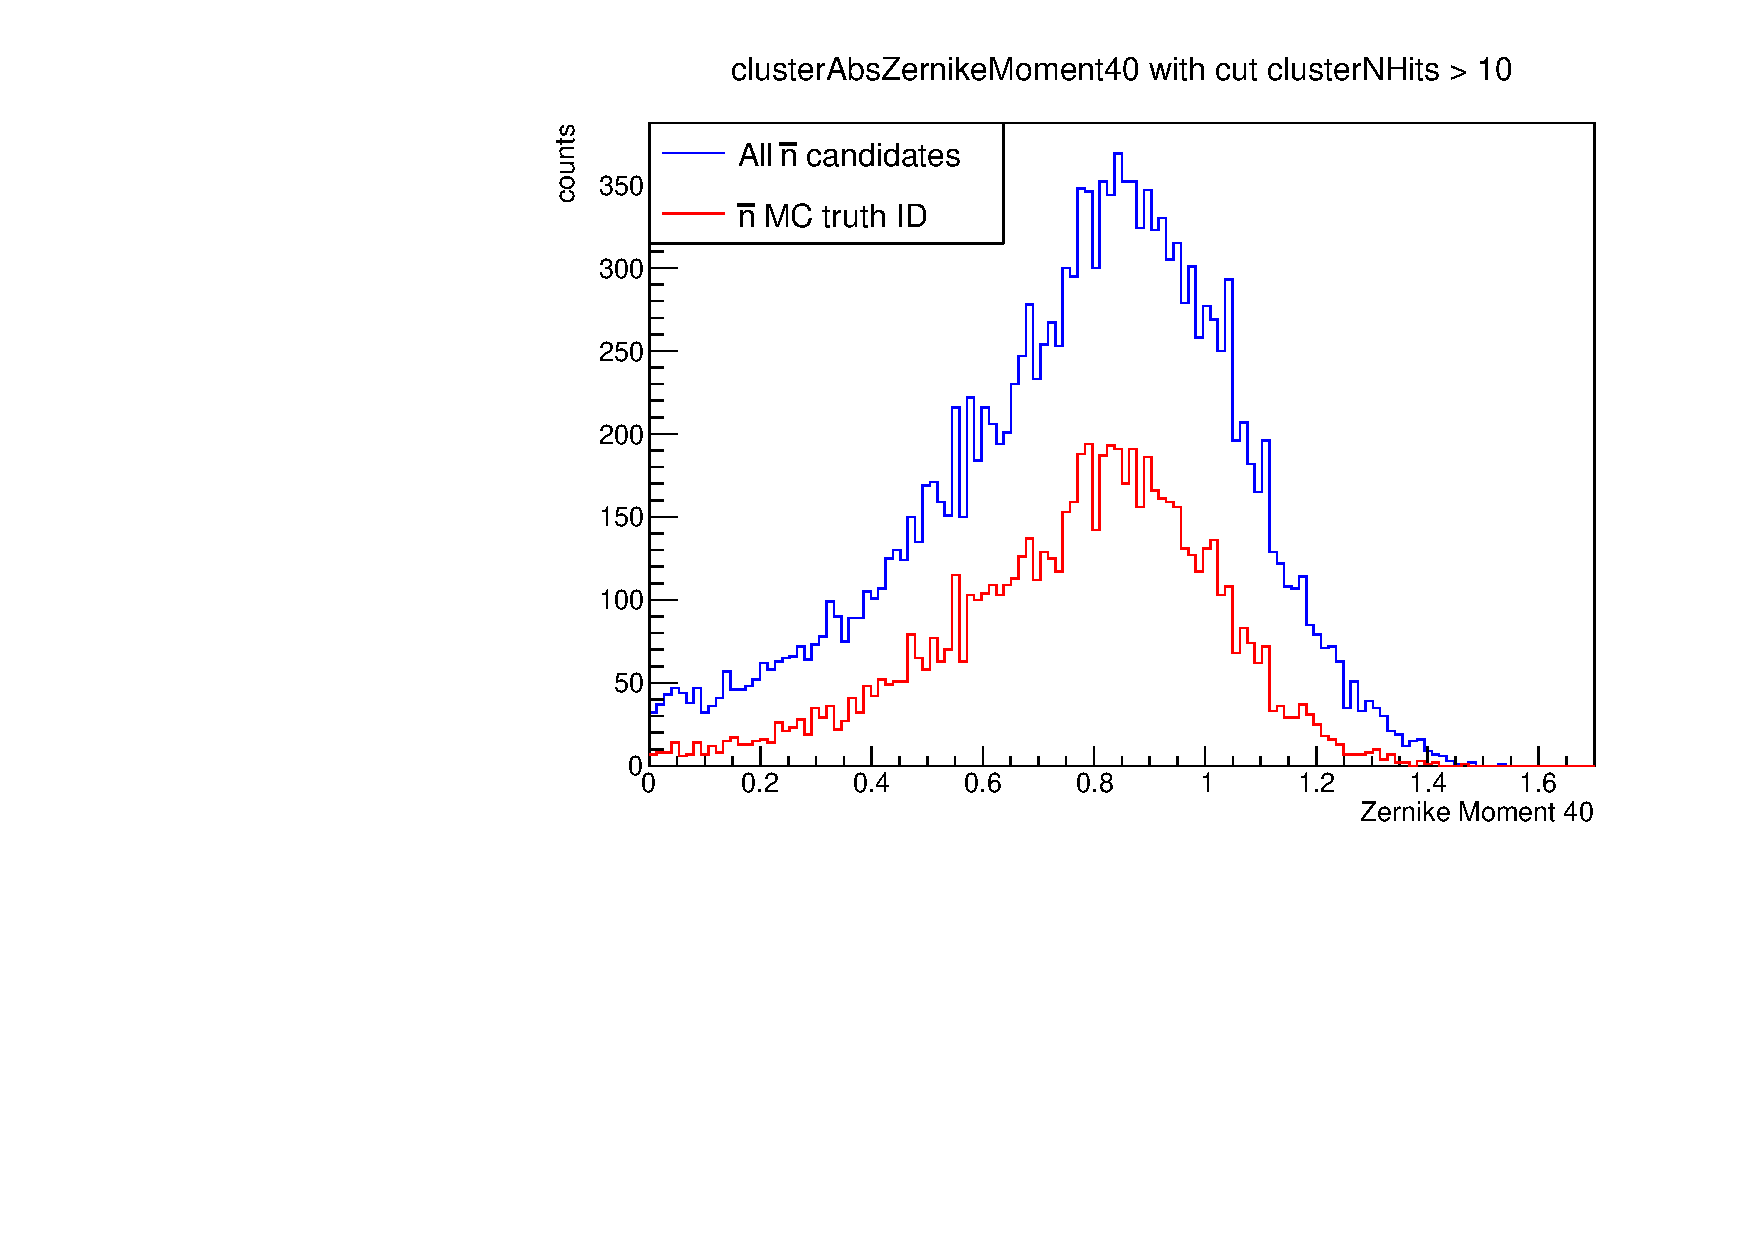
\includegraphics[width=0.49\textwidth]{nbar_MC/images/clusterAbsZernikeMoment40_hitscut_isr.pdf}
    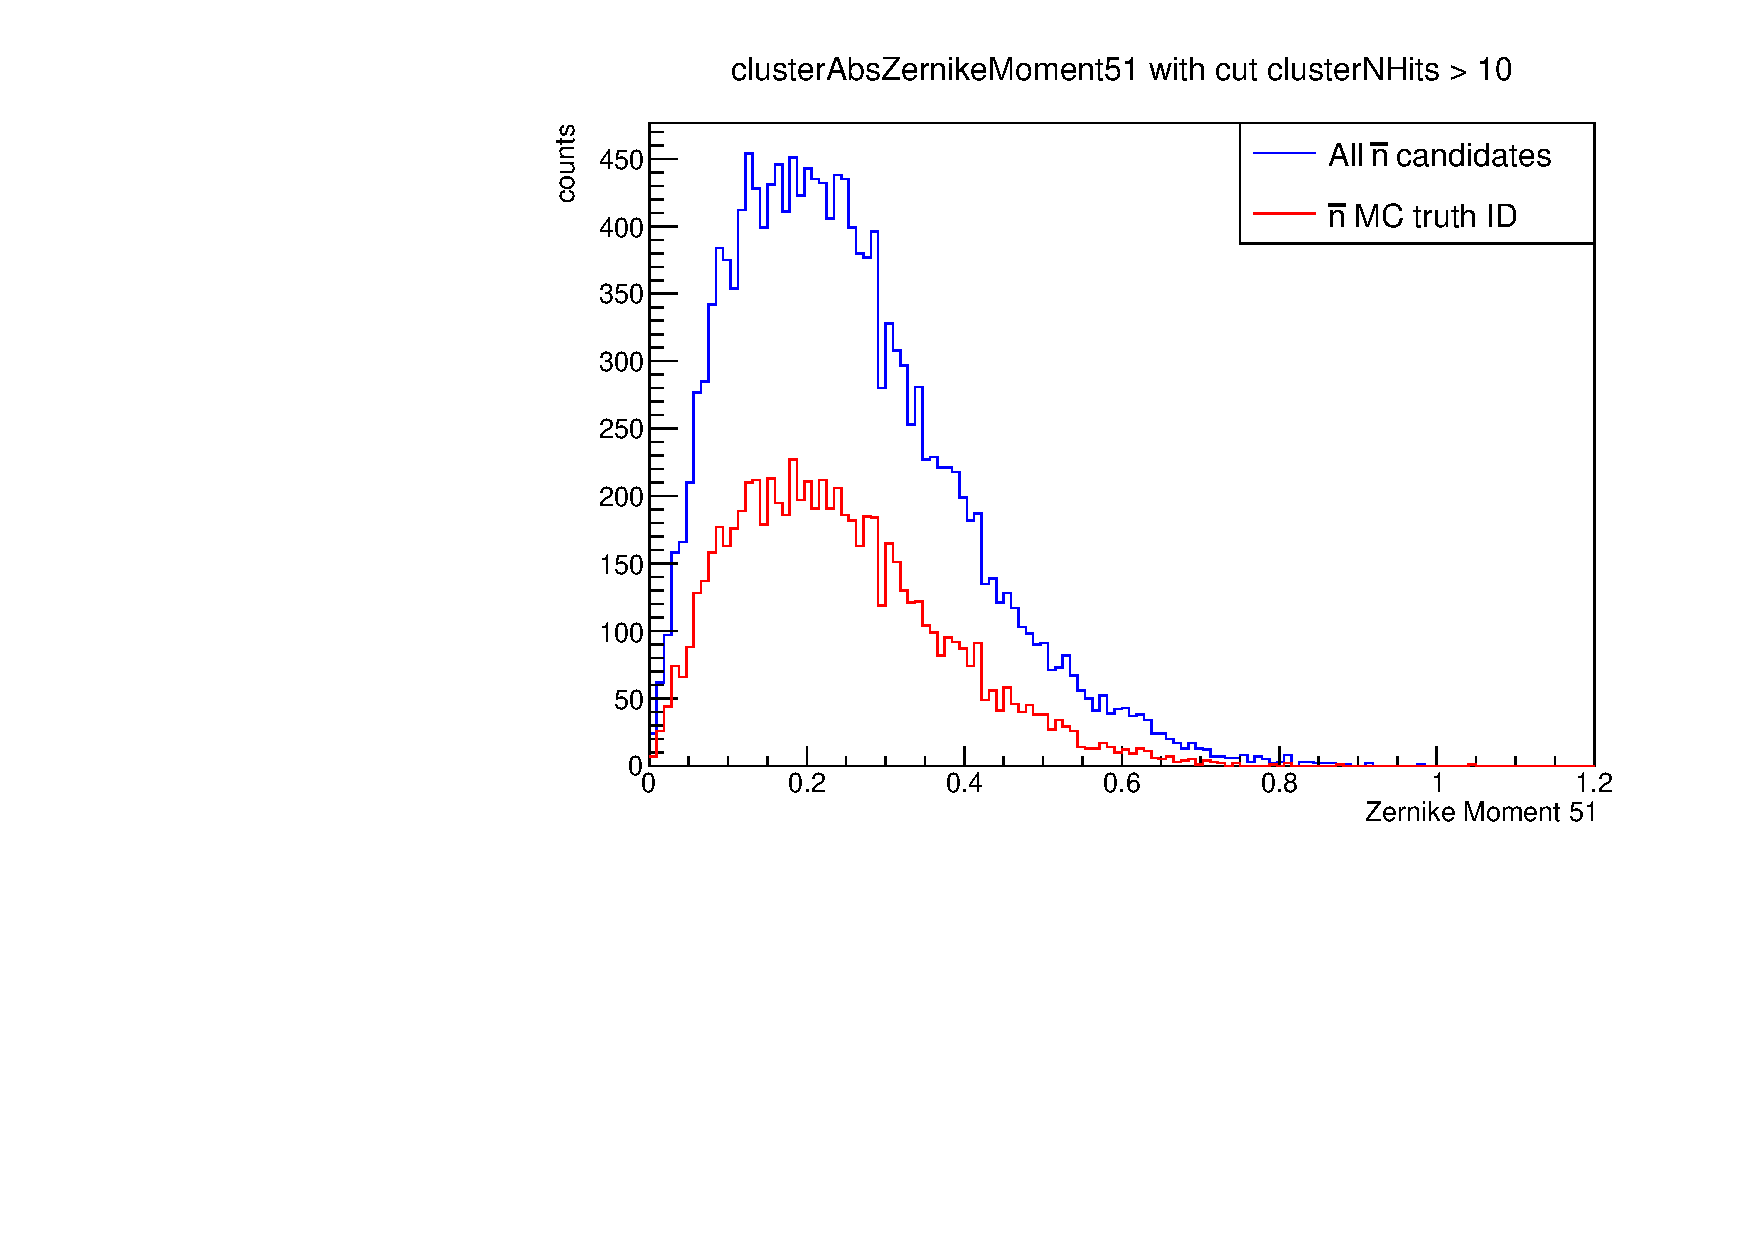
\includegraphics[width=0.49\textwidth]{nbar_MC/images/clusterAbsZernikeMoment51_hitscut_isr.pdf}
    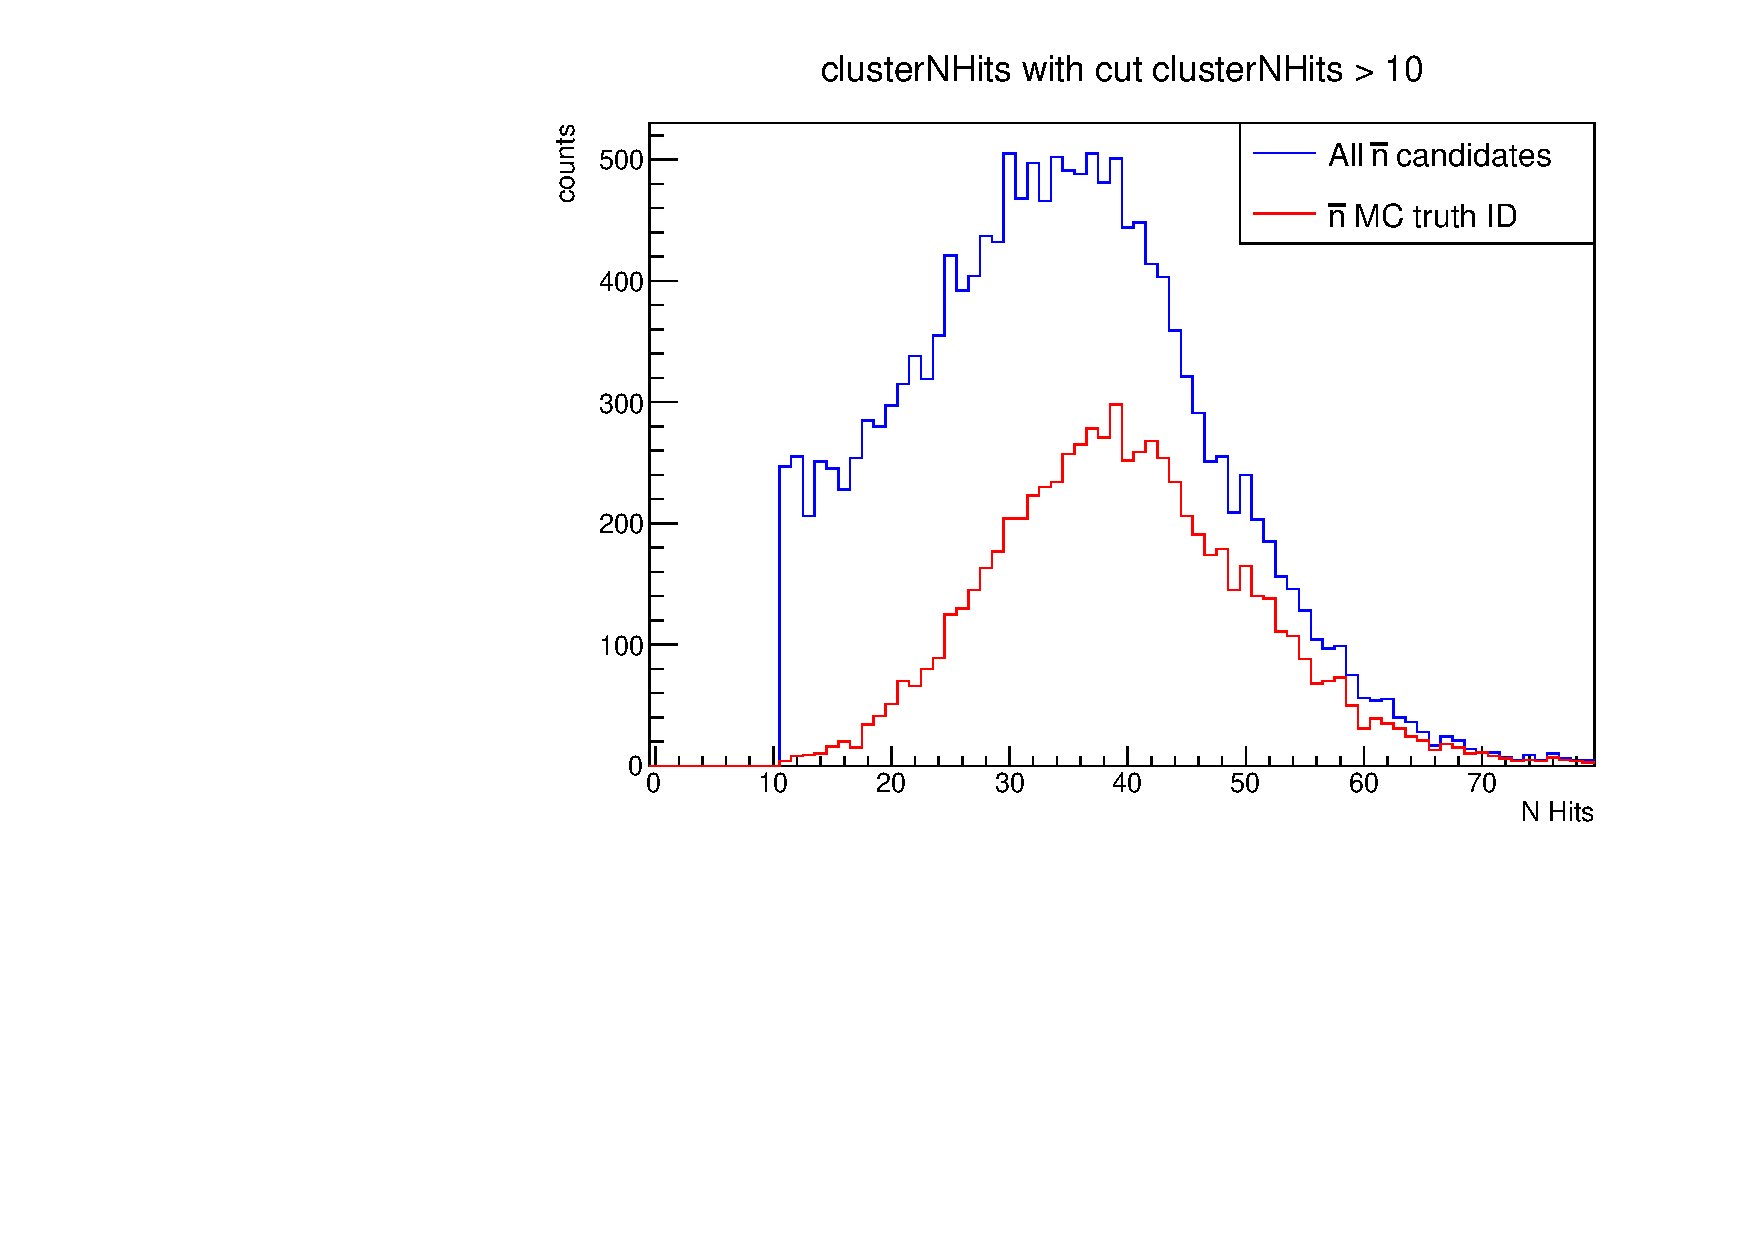
\includegraphics[width=0.49\textwidth]{nbar_MC/images/clusterNHits_hitscut_isr.pdf}
   
     \caption{Comparison of reconstructed cluster variables for all $\bar{n}$ candidates versus those associated with $\bar{n}$ particles by Monte Carlo truth Monte Carlo PDG = -2112 (ISR case). Cut $clusterNHits > 10$ is performed}
     
     \label{fig:cluster_ISR_NHits}

\end{figure}

\newpage
The obtained cluster variables in NO ISR case are shown below:
 \begin{figure}[H]
    \centering
    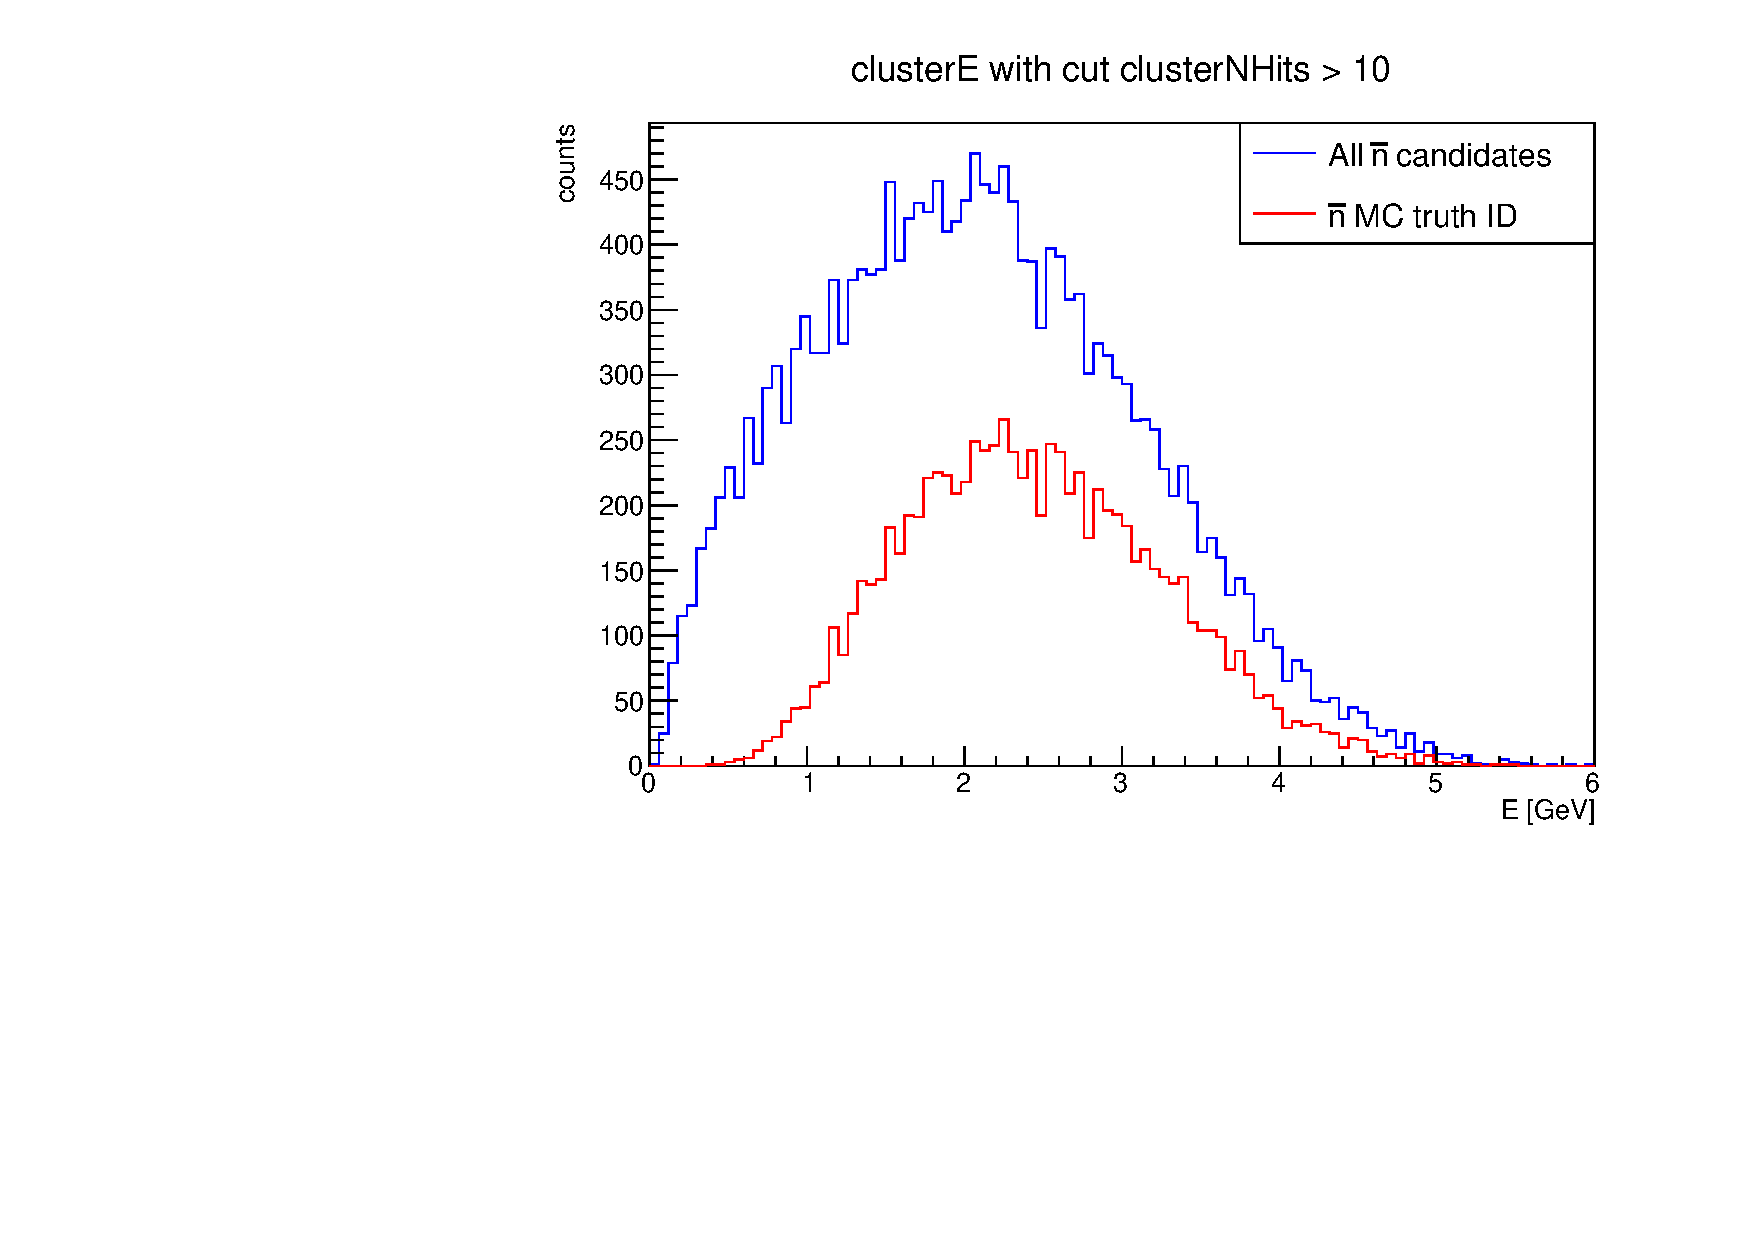
\includegraphics[width=0.49\textwidth]{nbar_MC/images/clusterE_hitscut_nog.pdf}
    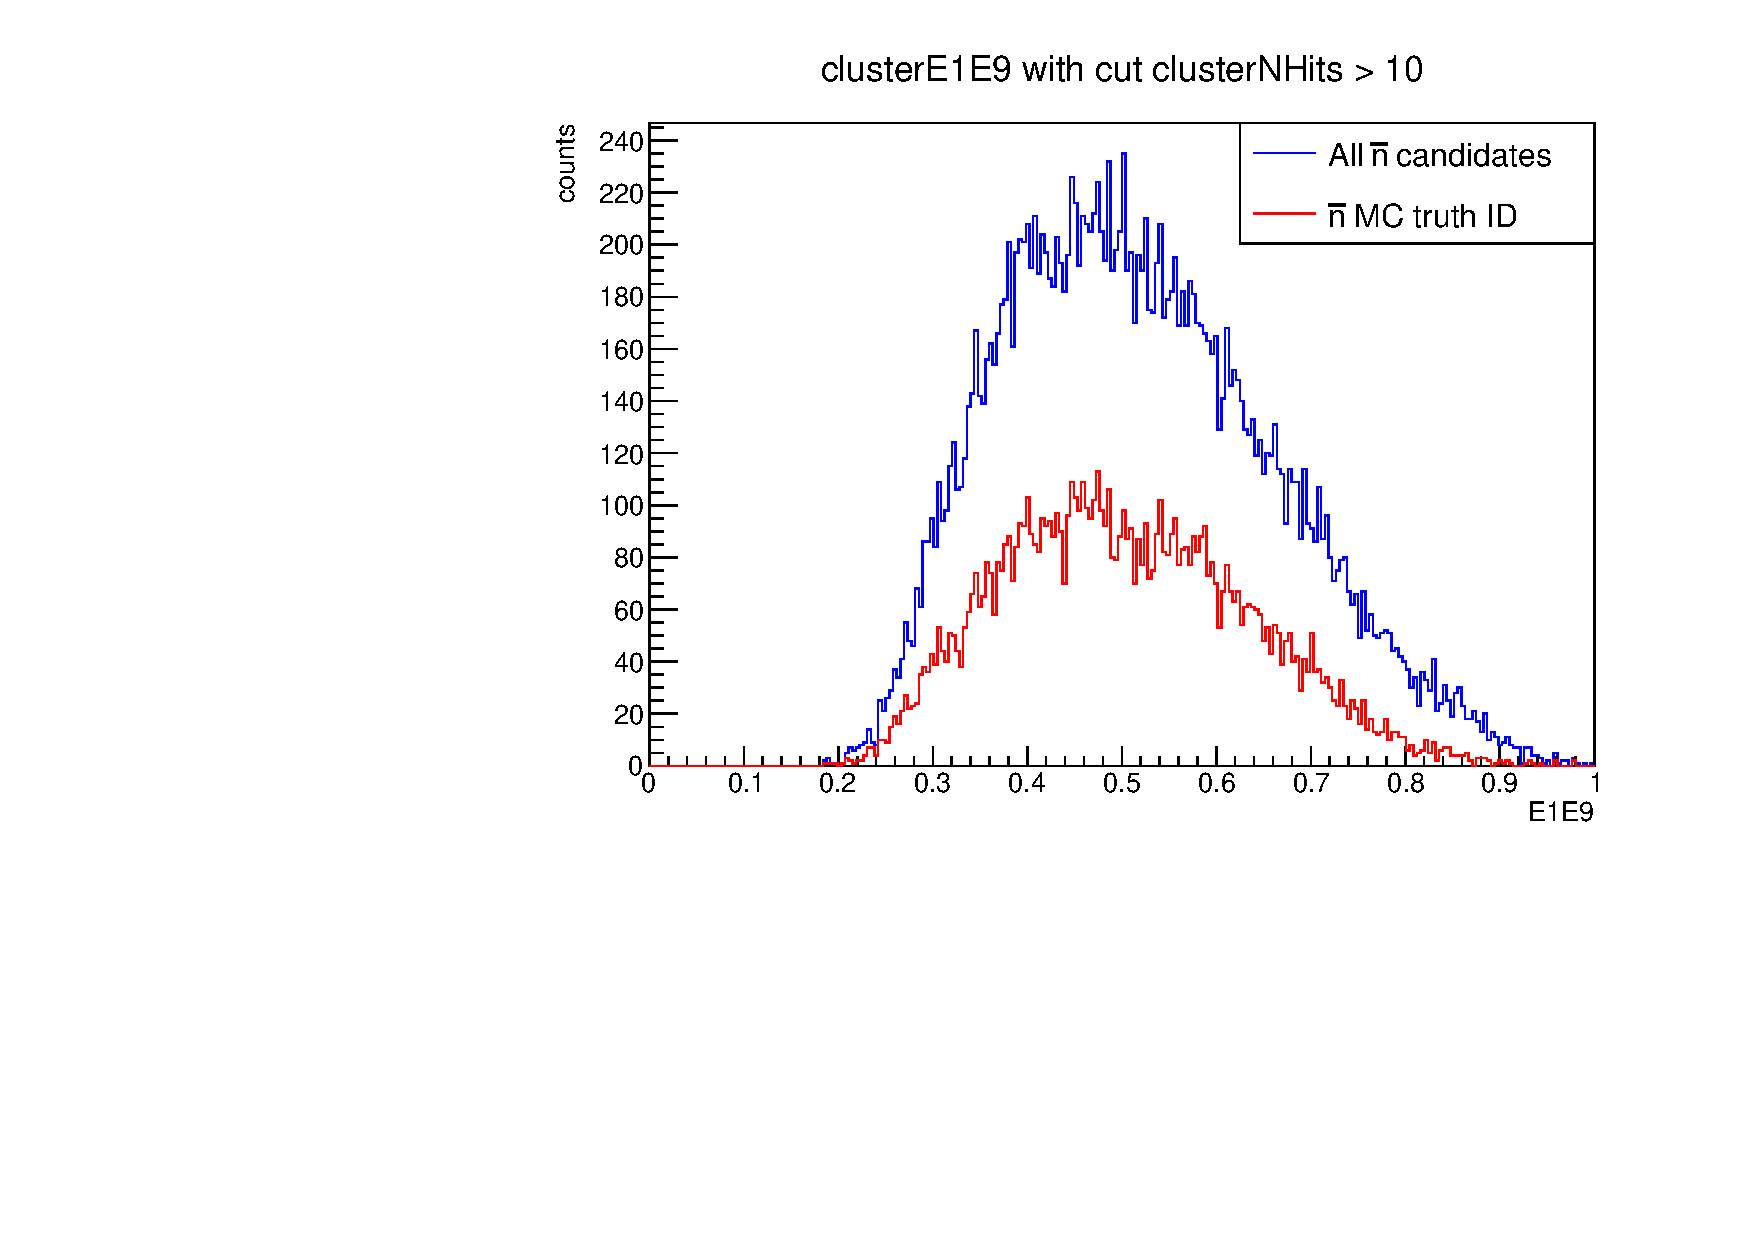
\includegraphics[width=0.49\textwidth]{nbar_MC/images/clusterE1E9_hitscut_nog.pdf}
    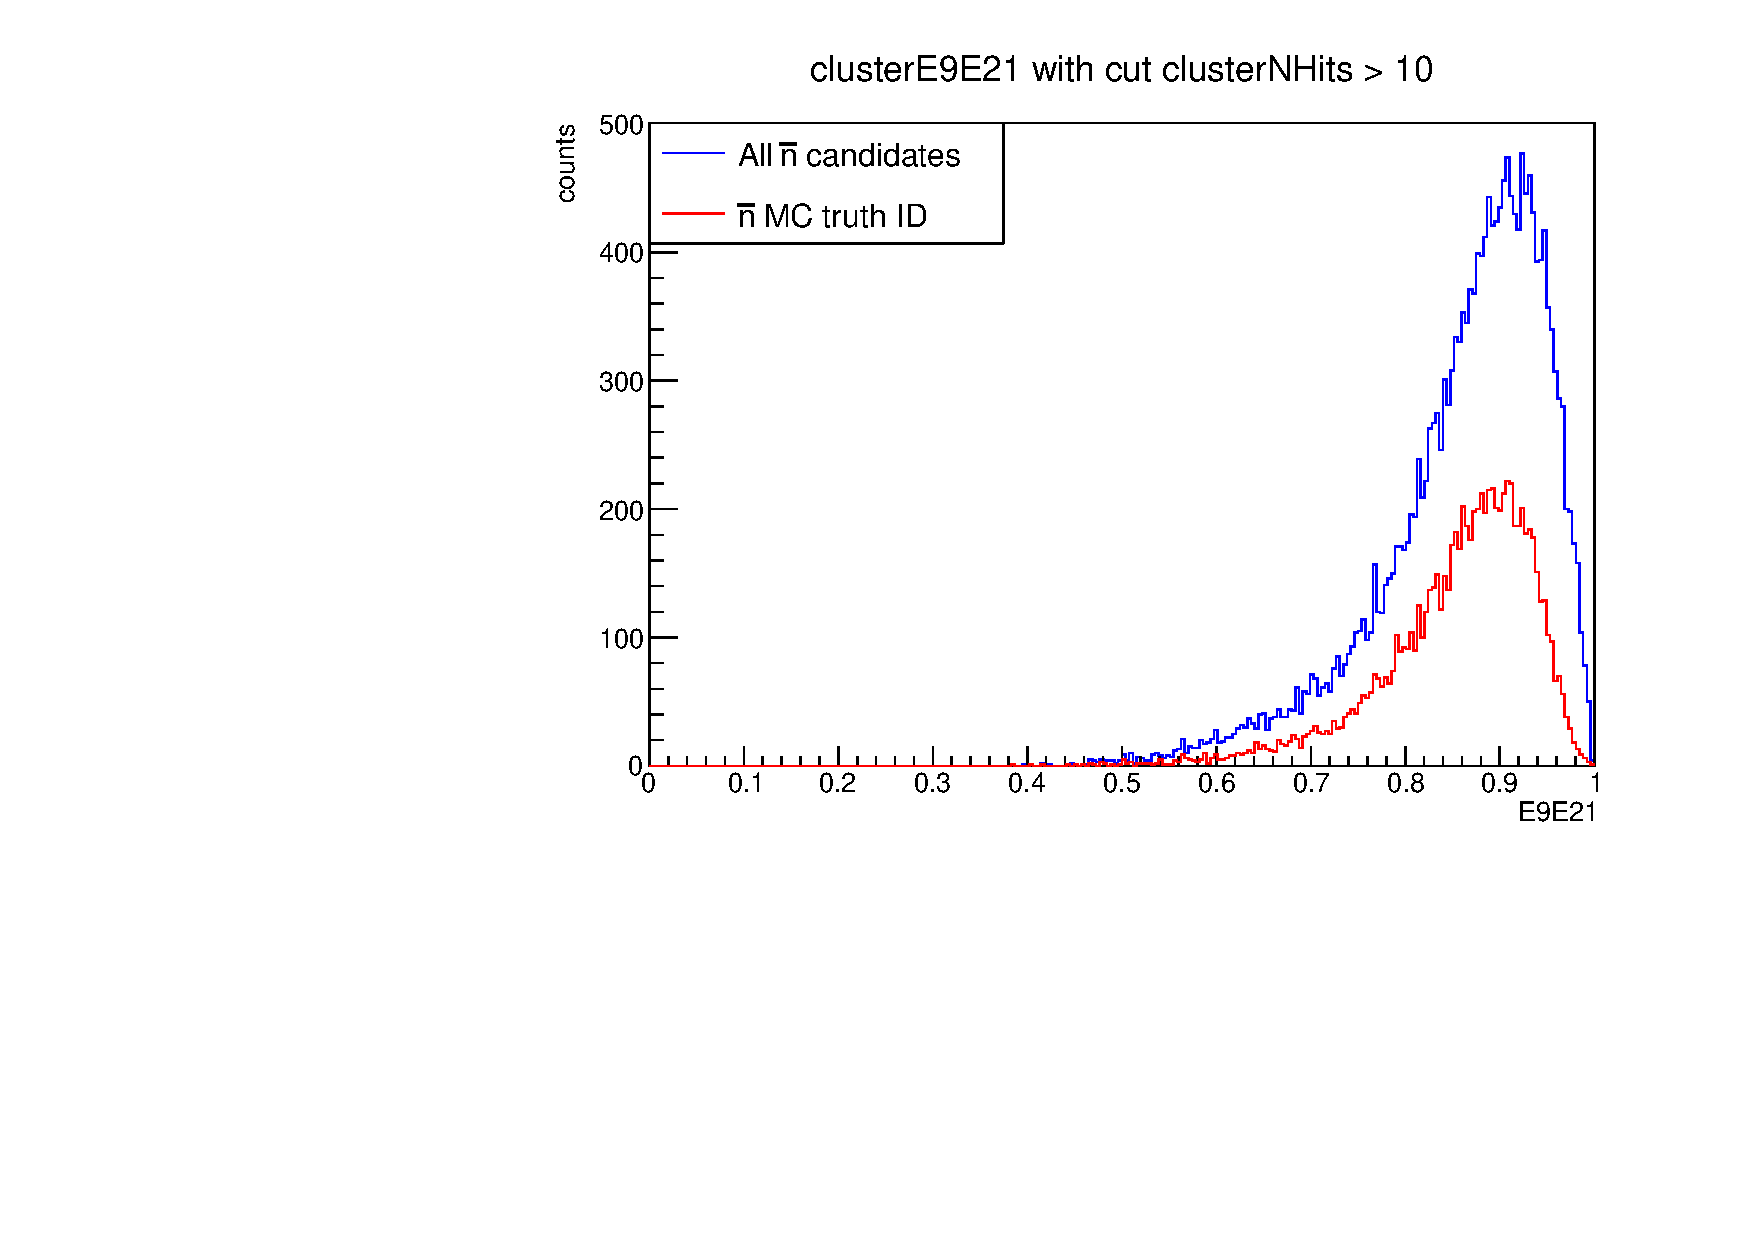
\includegraphics[width=0.49\textwidth]{nbar_MC/images/clusterE9E21_hitscut_nog.pdf}
    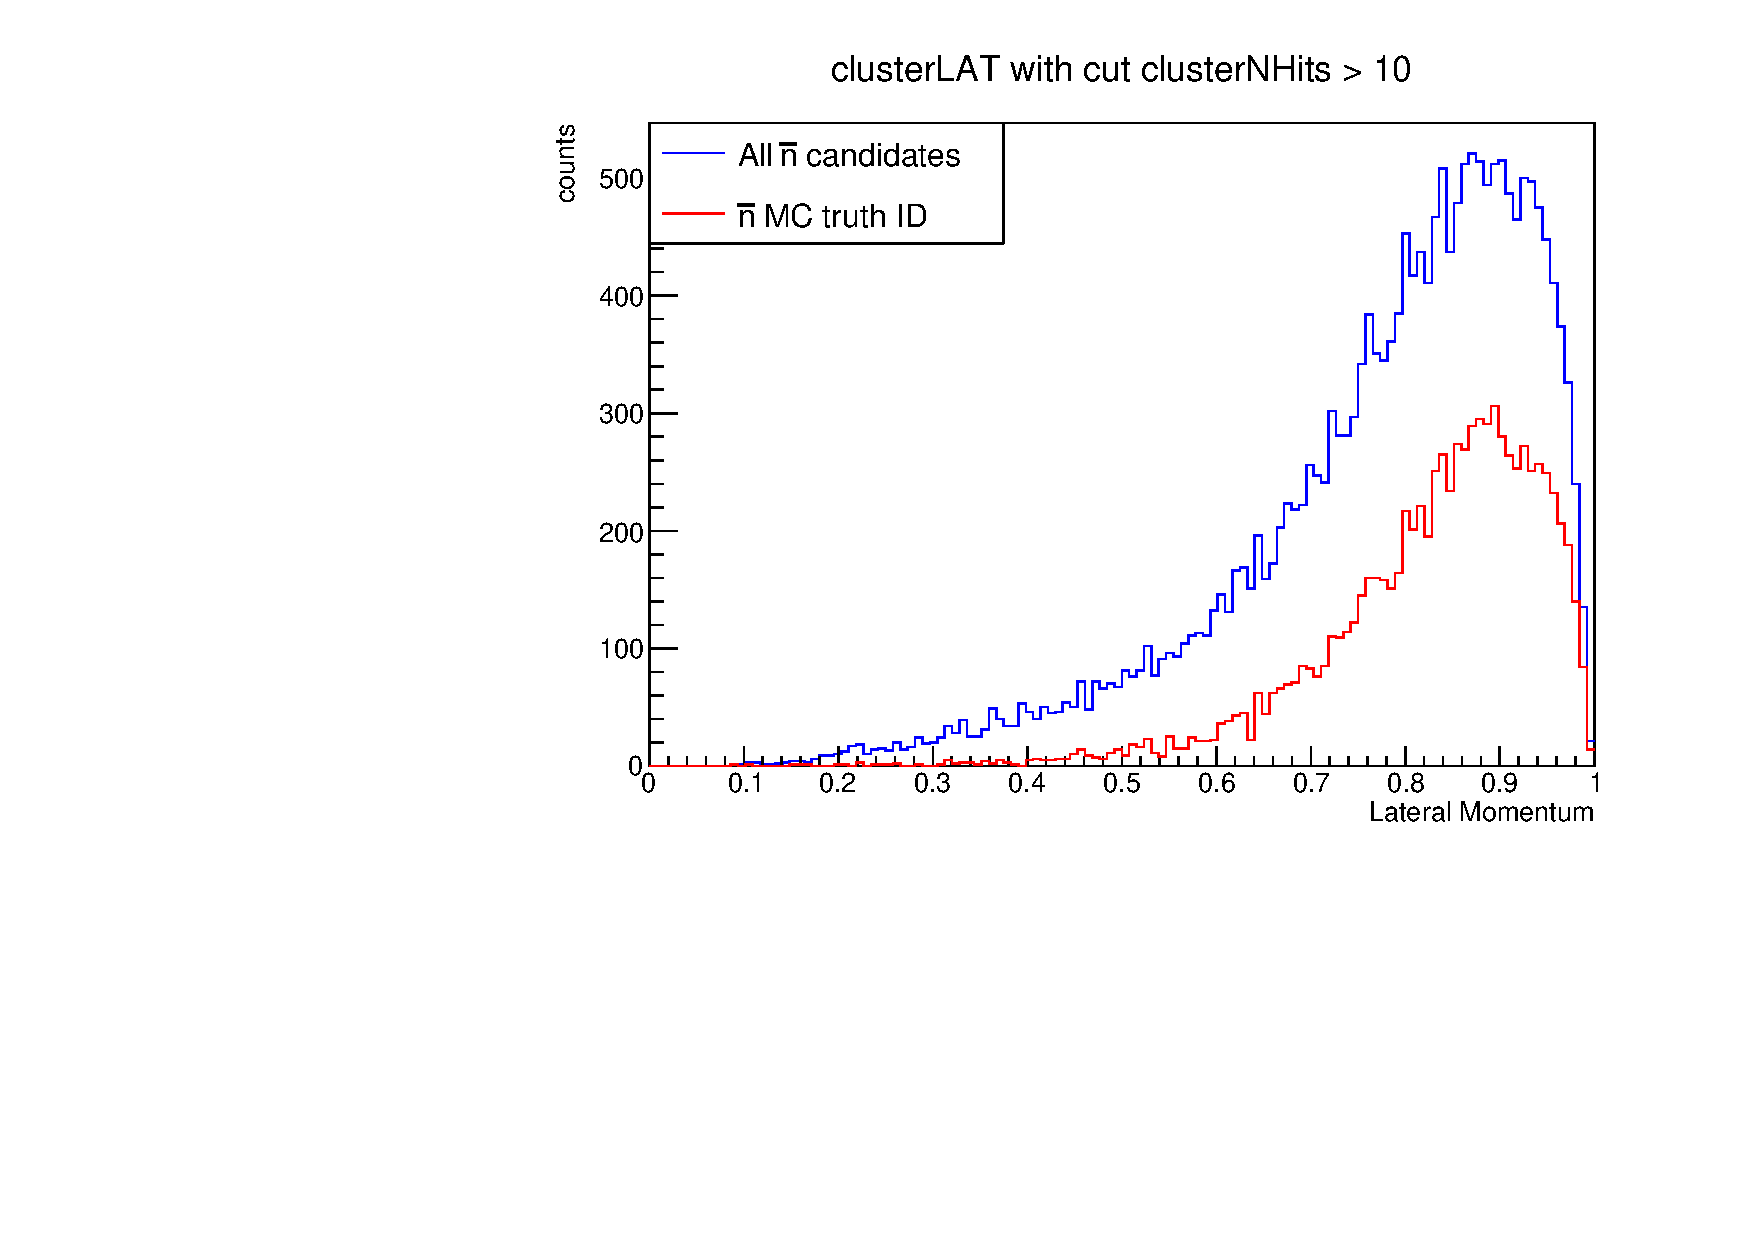
\includegraphics[width=0.49\textwidth]{nbar_MC/images/clusterLAT_hitscut_nog.pdf}
    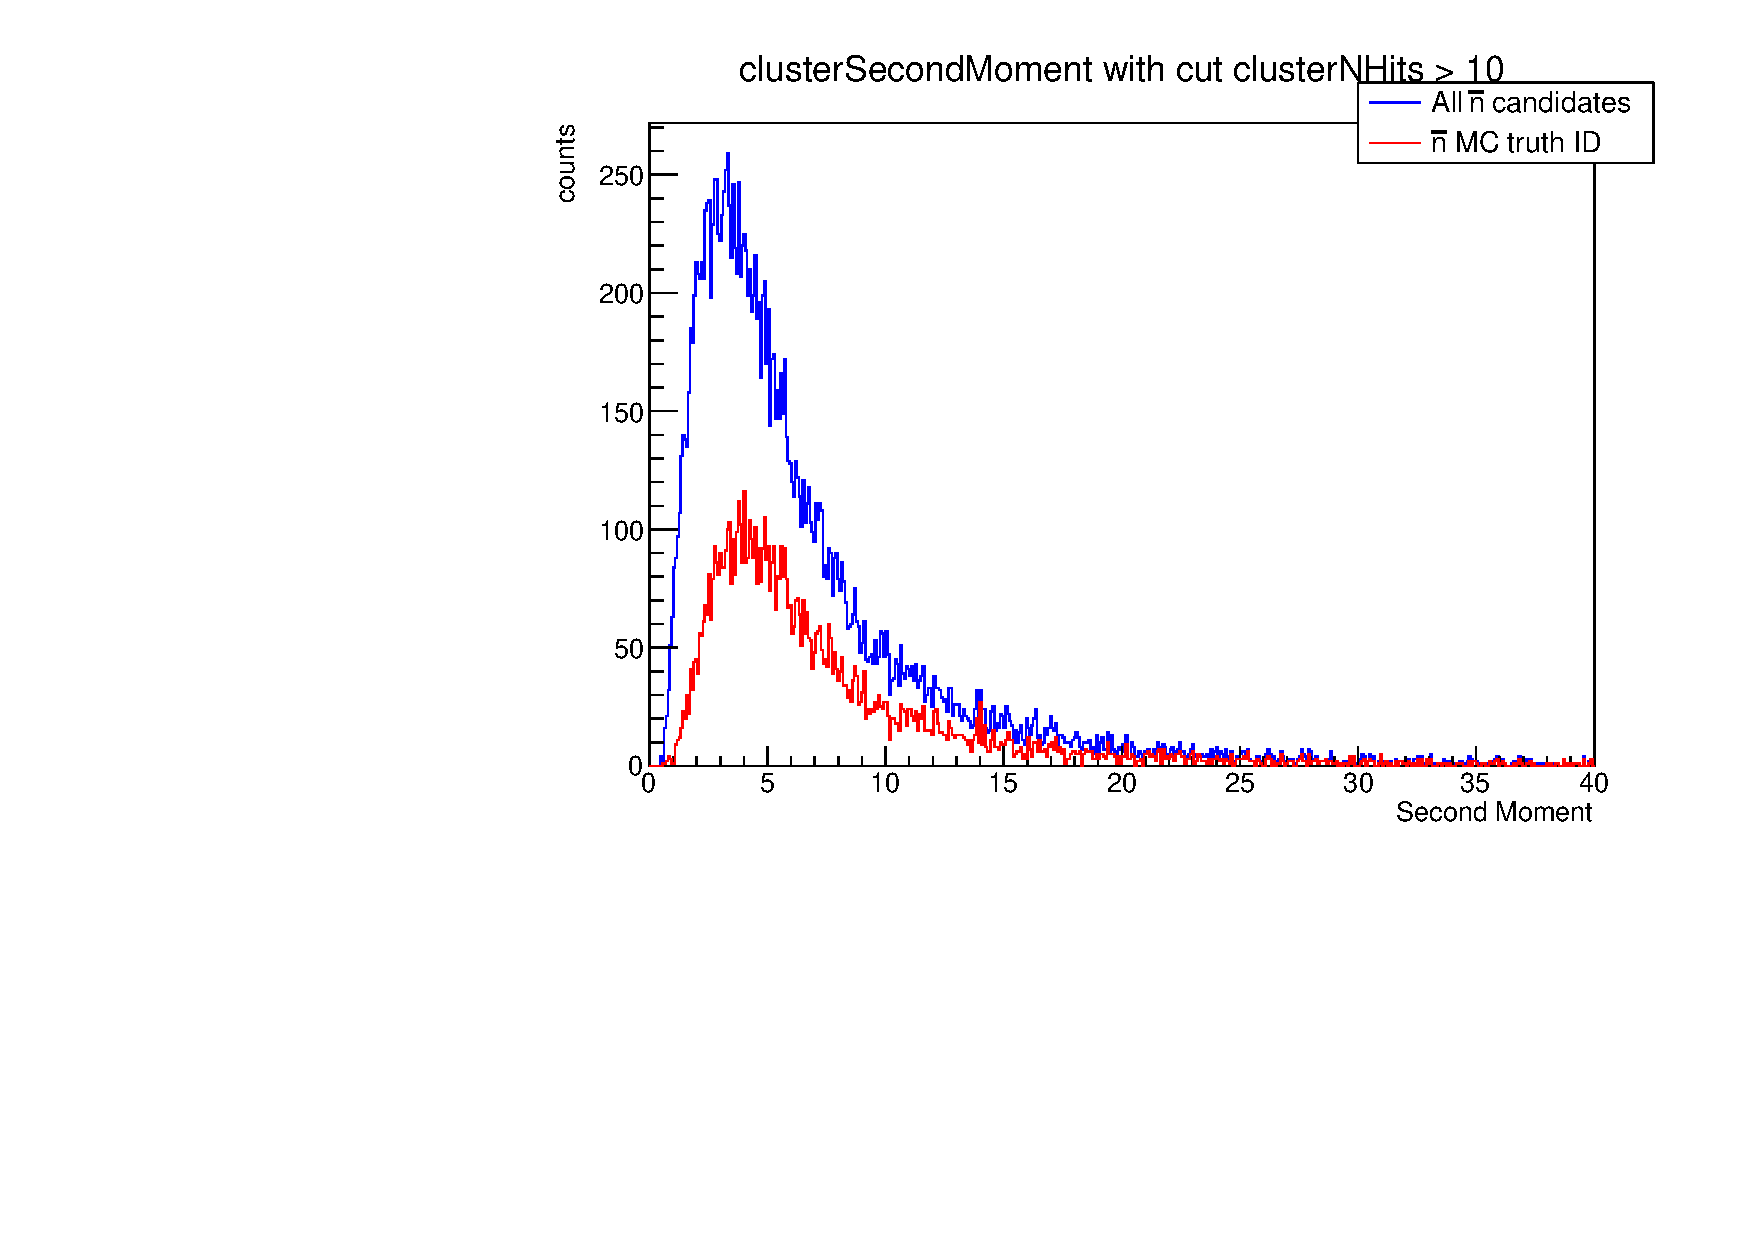
\includegraphics[width=0.49\textwidth]{nbar_MC/images/clusterSecondMoment_hitscut_nog.pdf}
    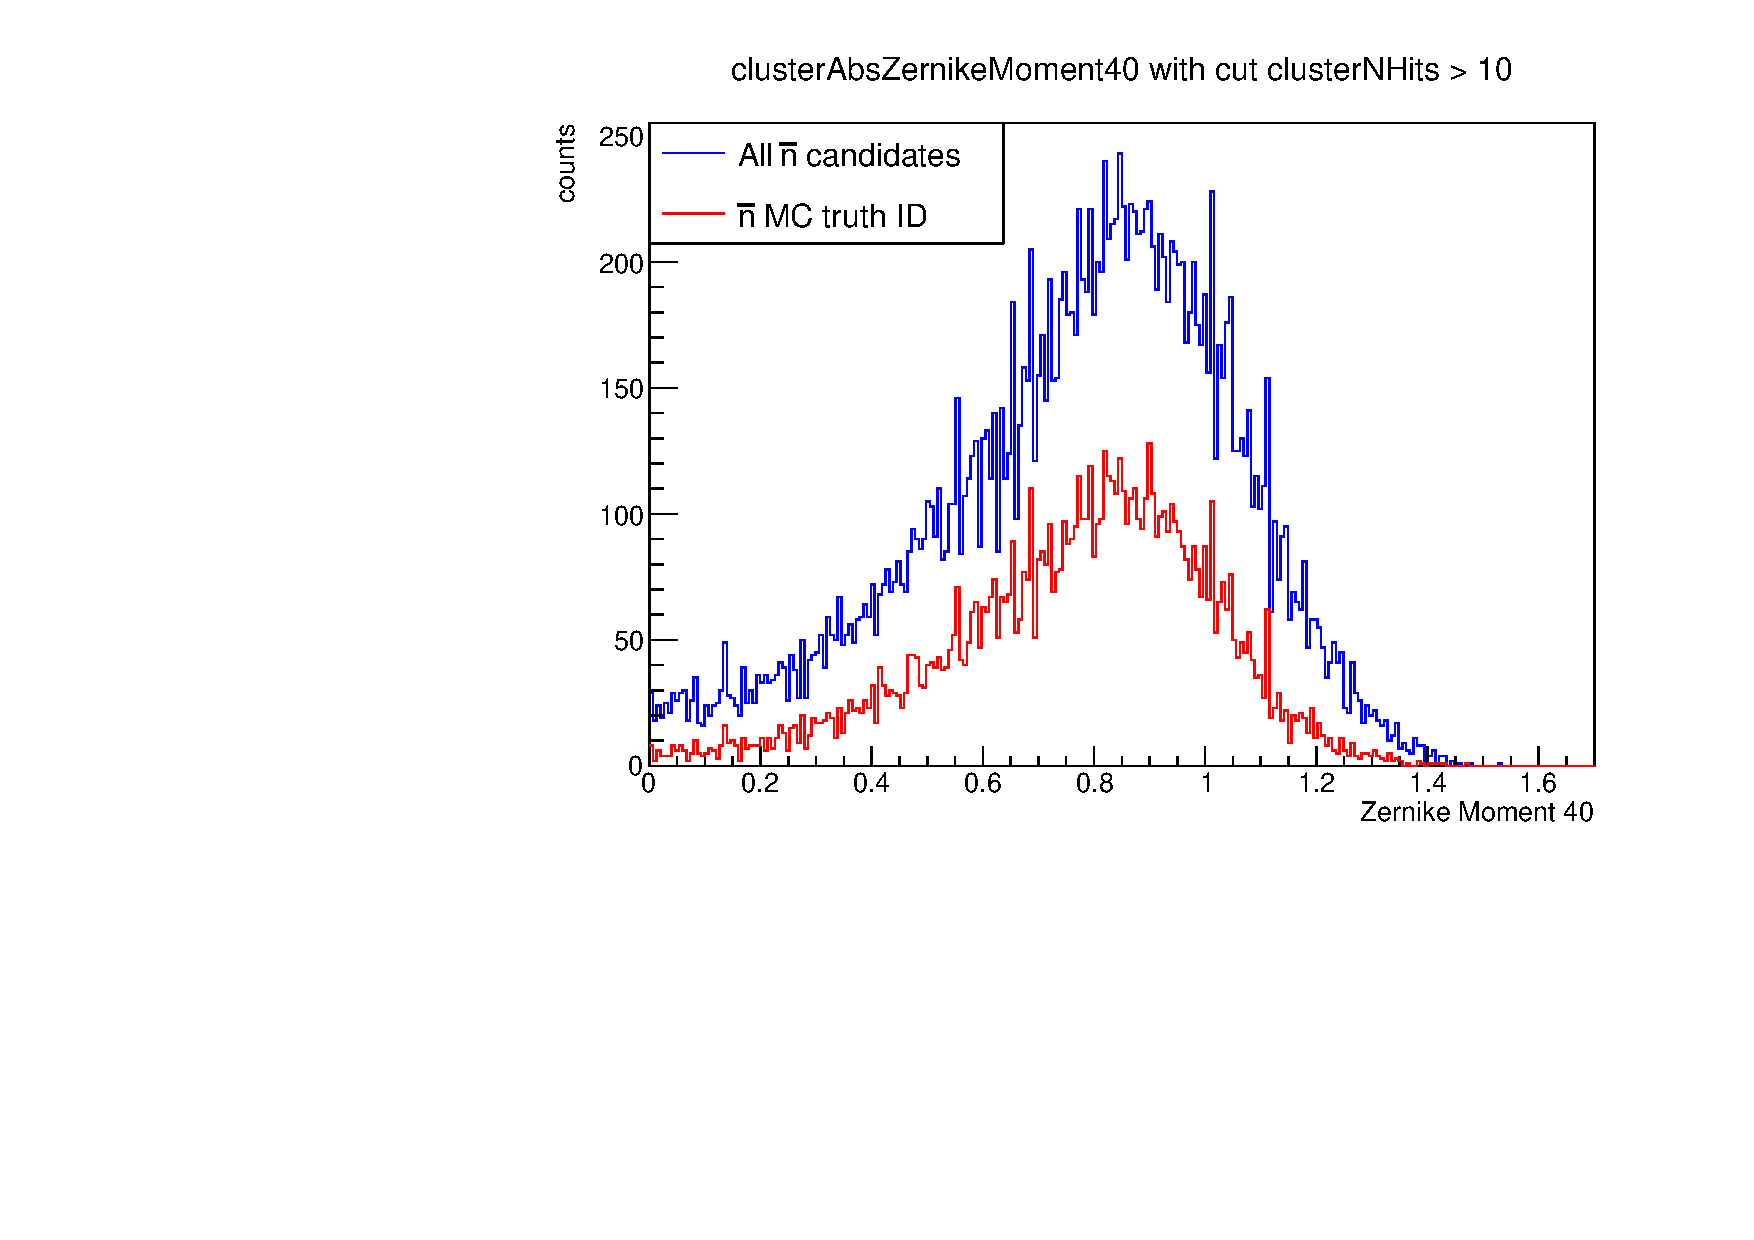
\includegraphics[width=0.49\textwidth]{nbar_MC/images/clusterAbsZernikeMoment40_hitscut_nog.pdf}
    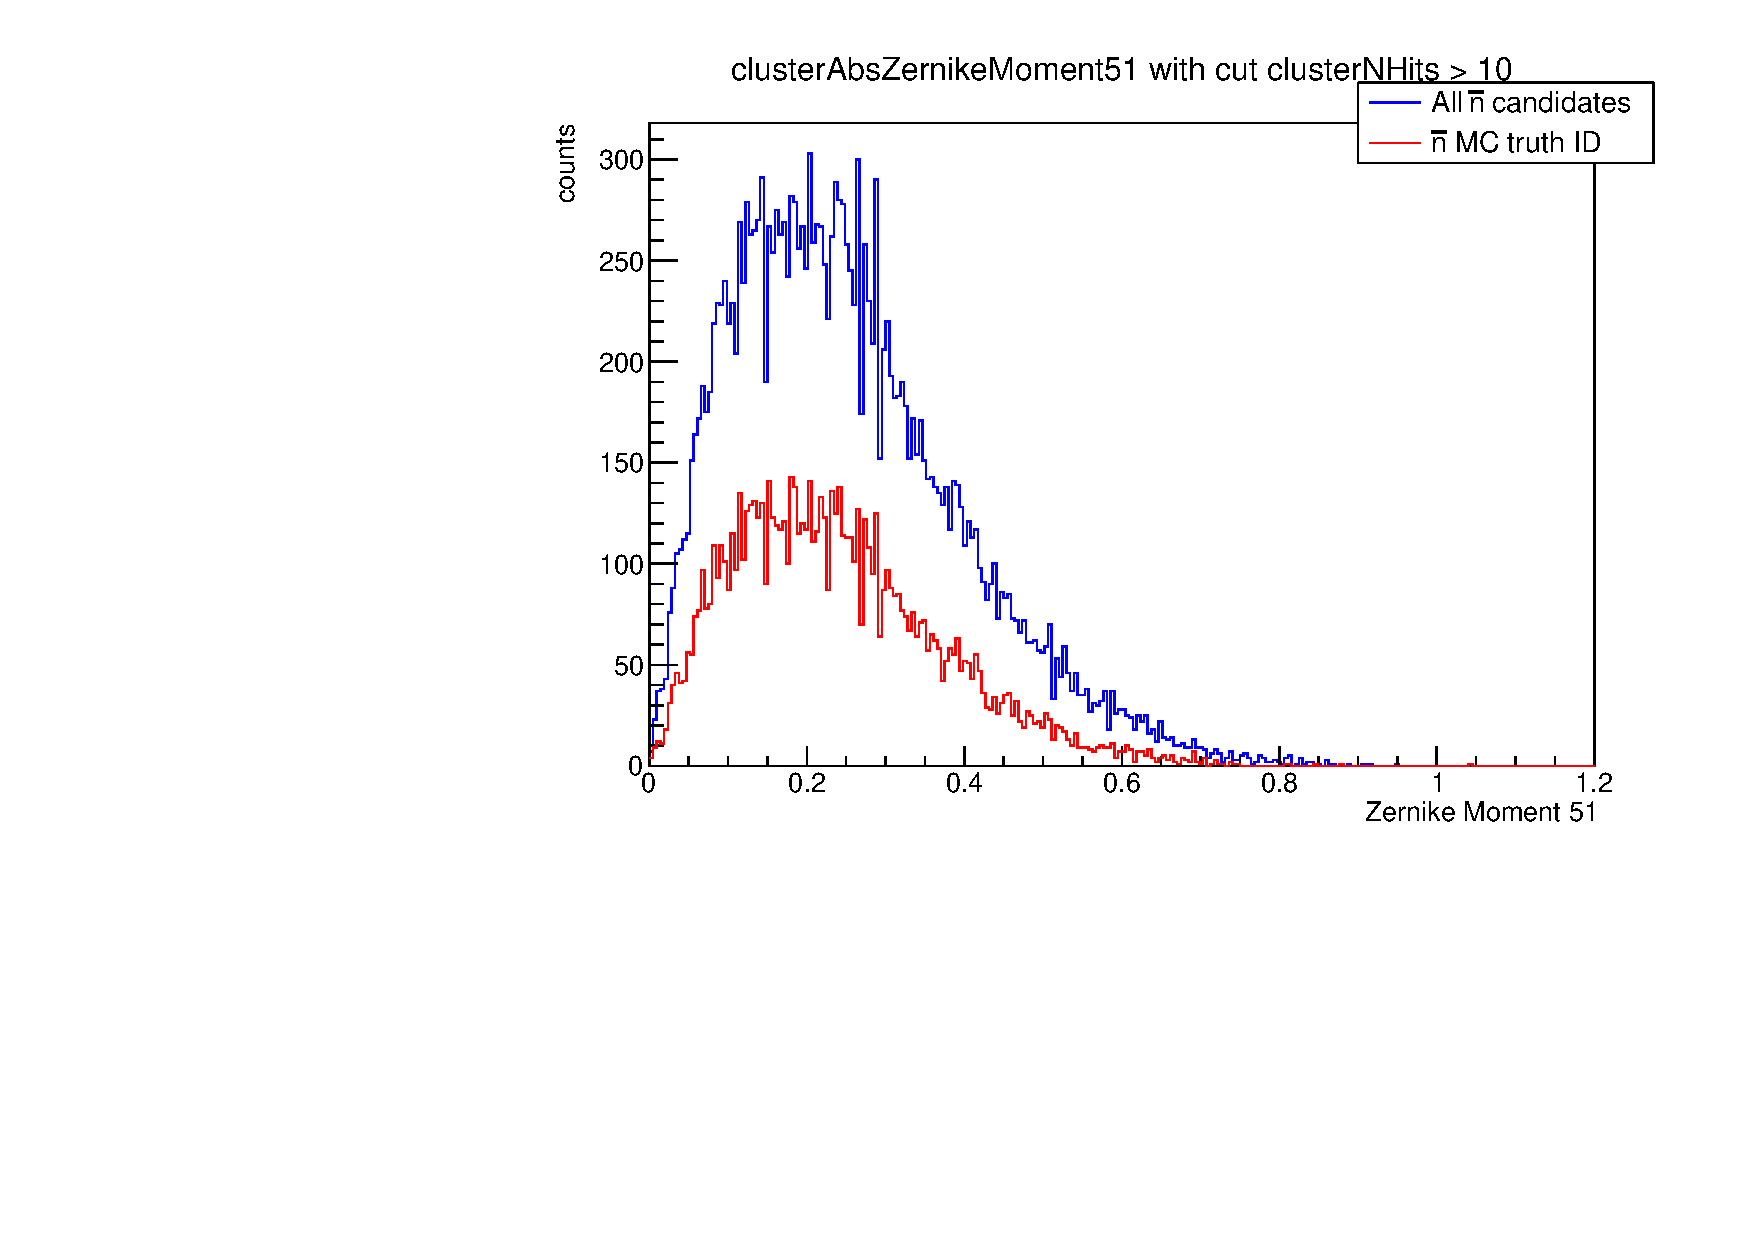
\includegraphics[width=0.49\textwidth]{nbar_MC/images/clusterAbsZernikeMoment51_hitscut_nog.pdf}
    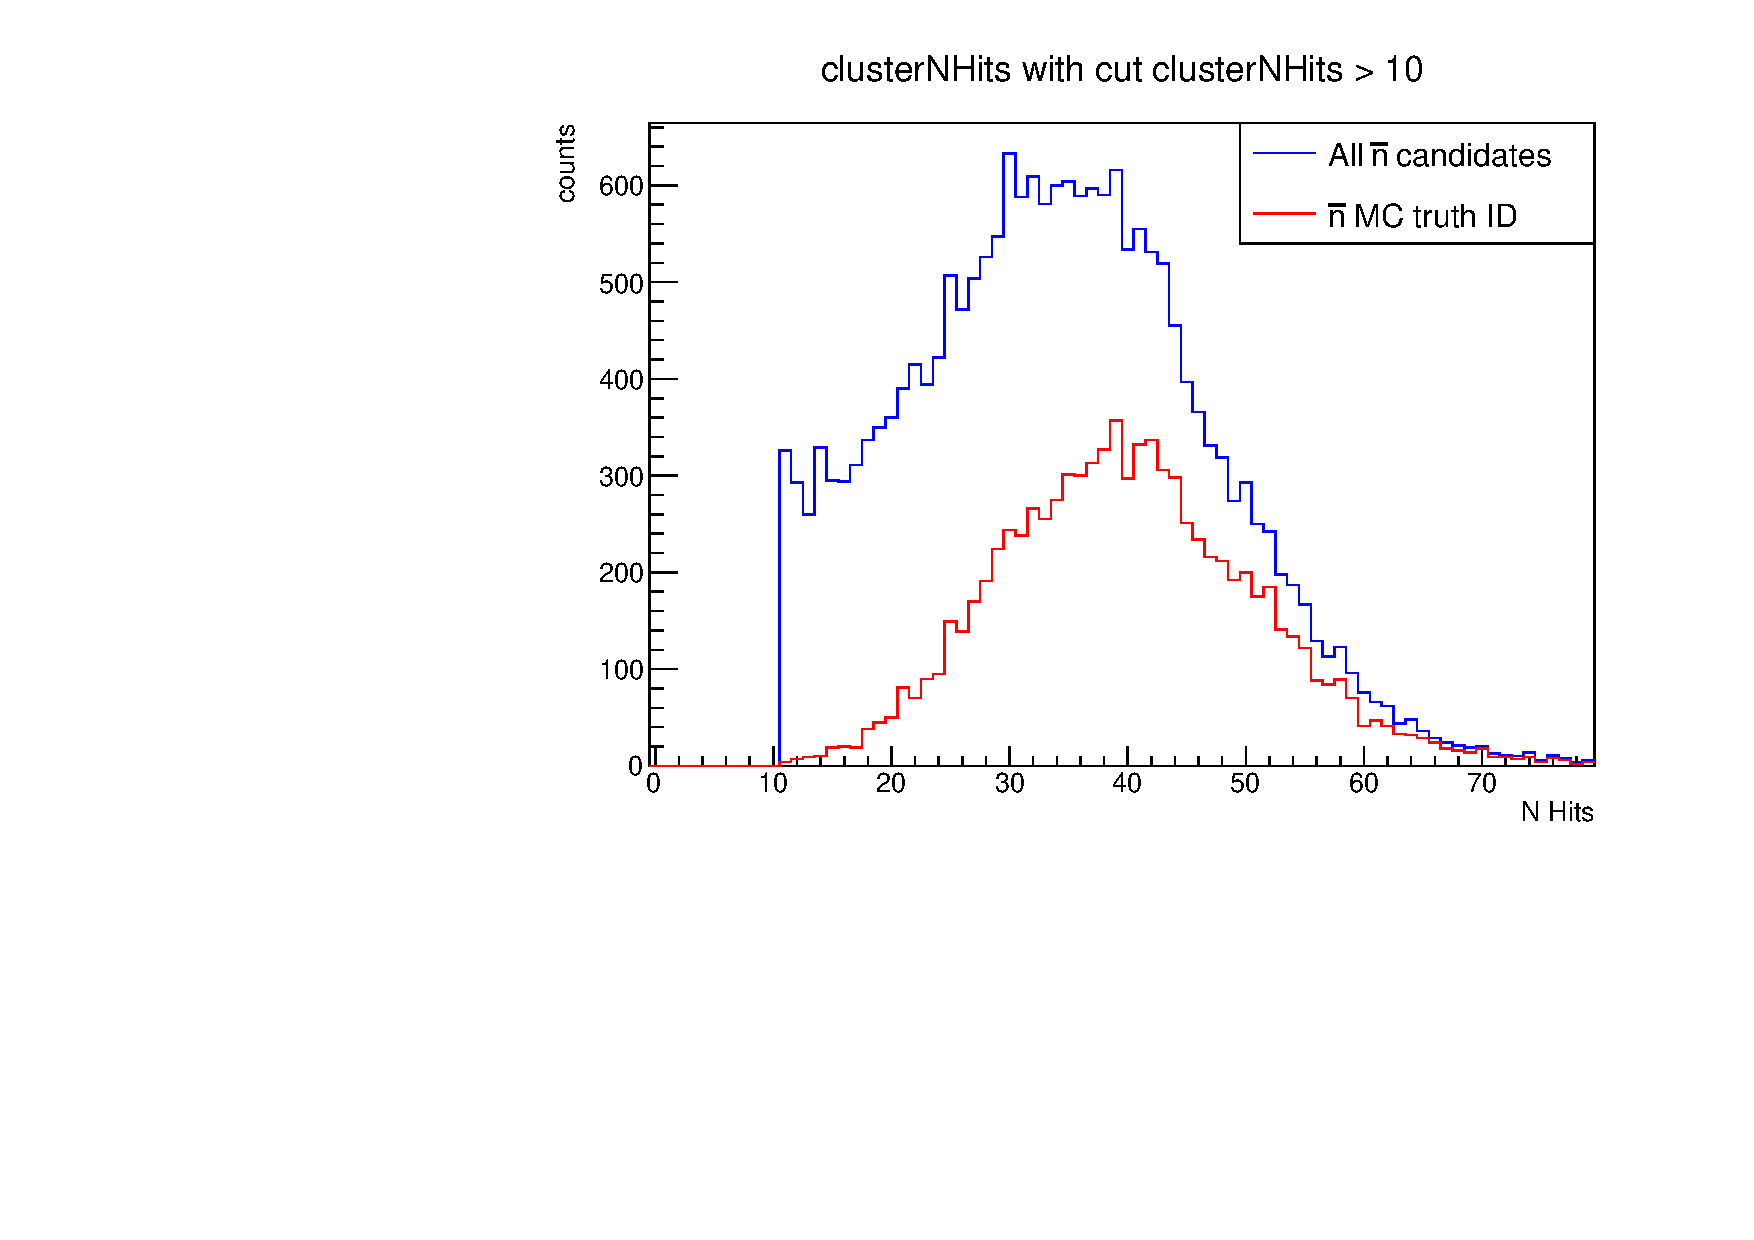
\includegraphics[width=0.49\textwidth]{nbar_MC/images/clusterNHits_hitscut_nog.pdf}
   
     \caption{Comparison of reconstructed cluster variables for all $\bar{n}$ candidates versus those associated with $\bar{n}$ particles by Monte Carlo truth Monte Carlo PDG = -2112 (NO ISR case). Cut $clusterNHits > 10$ is performed}
     
     \label{fig:cluster_NOISR_NHits}

\end{figure}

\newpage

\subsubsection{Cluster variables in different ECL regions}
As described in Chapter 3, the Belle II detector is divided into barrel and forward/backward end-cap regions. It would be interesting to study the reconstructed cluster variables in each ECL region separately. Since the ISR and NO ISR cases exhibit analogous shower shapes, only the latter is discussed here.
$\\$
The region hit distribution is shown below:
 \begin{figure}[H]
    \centering
    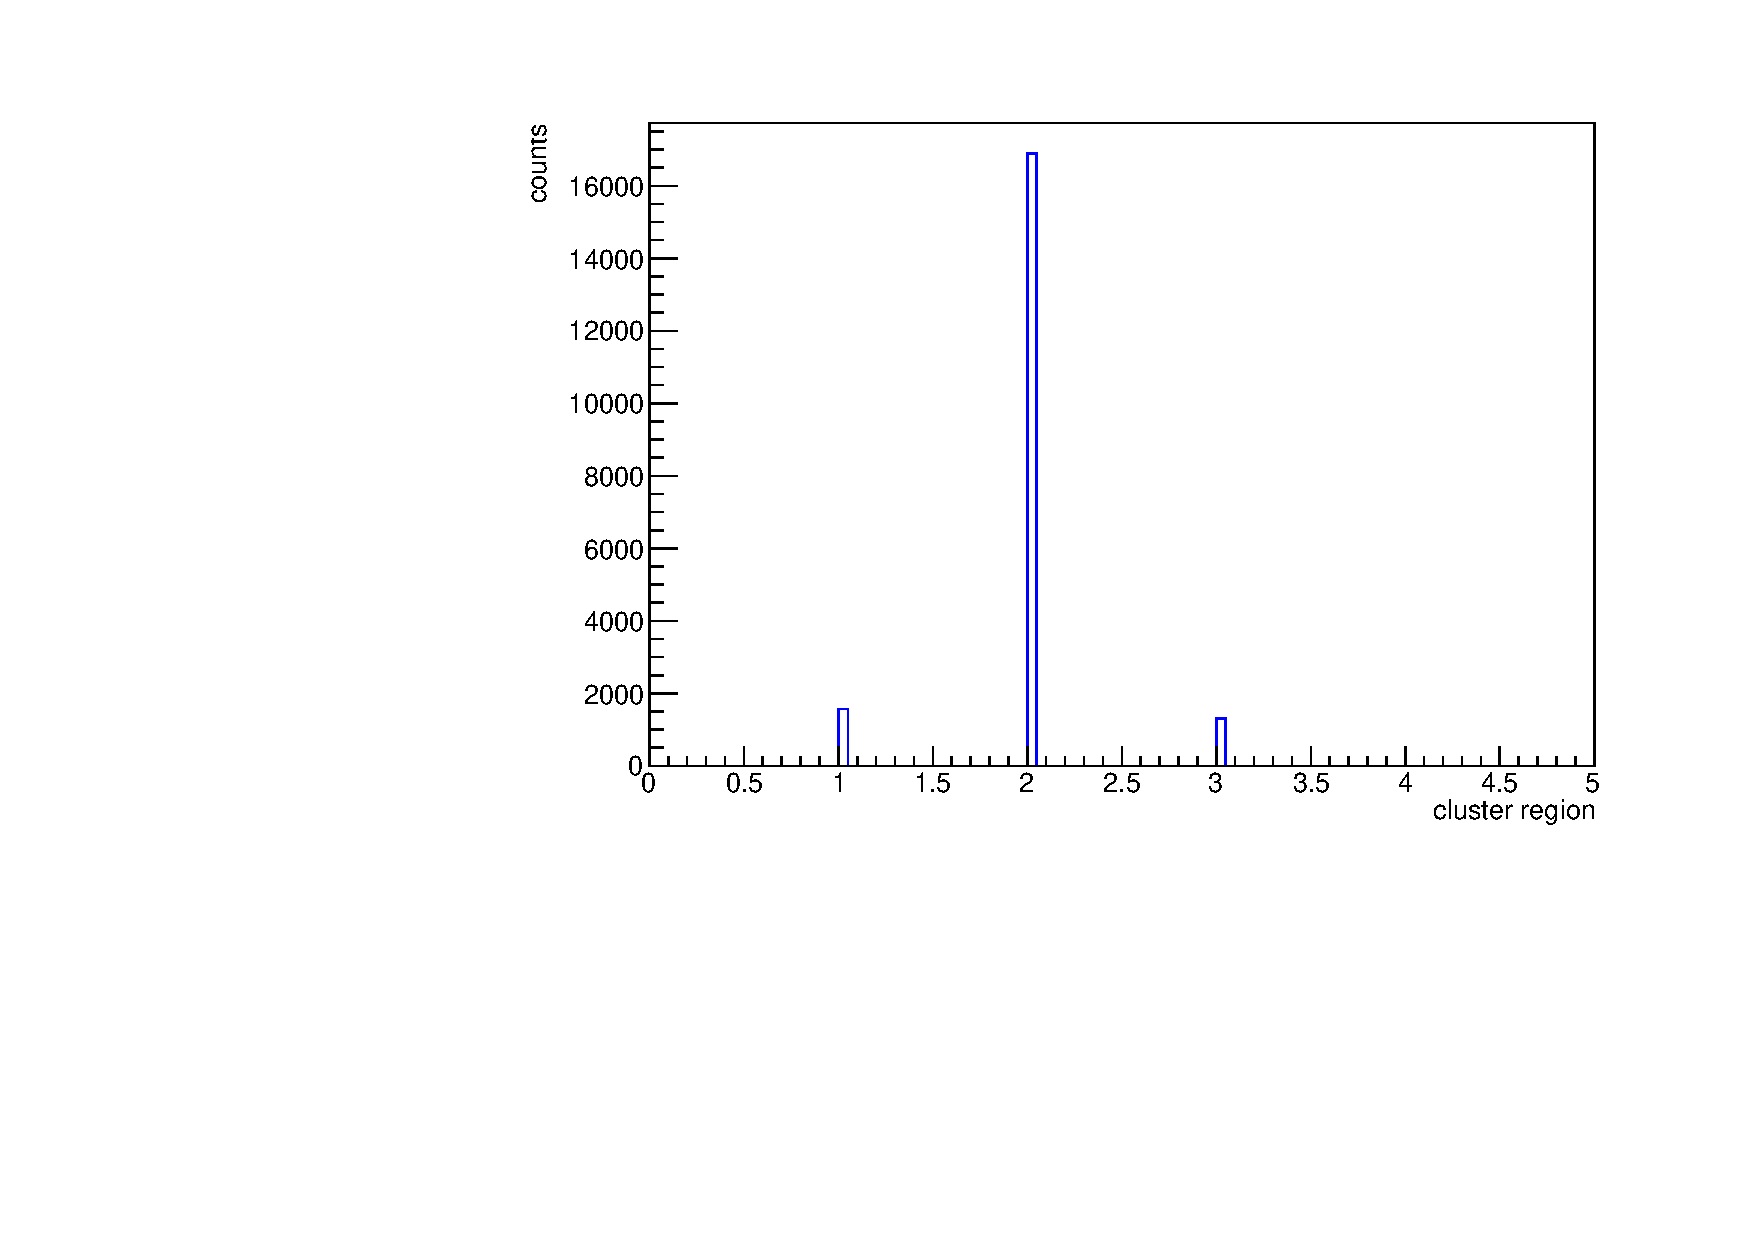
\includegraphics[width=0.80\textwidth]{nbar_MC/images/cluster_region.pdf}

     \caption{Different ECL regions contribution in neutral cluster associated to $\bar{n}$ candidates, where 1 is the forward region, 2 is the barrel region and 3 is the backward region. As expected, the barrel region is the most involved}

\end{figure}

As observed in Fig.~\ref{fig:cluster_region}, the cluster variable associated to all the reconstructed  $\bar{n}$ shapes are consistent across all ECL regions. 
$\\$
However a slight difference can be noted for cluster energy and number of hits variables. In fact, these two exhibit a shift toward lower values in the forward region, reflecting the Lorentz boost of the center-of-mass. In any case, the barrel region contains the majority of ECL clusters, as expected.

\newpage
The obtained cluster variables in NO ISR case are shown below:
 \begin{figure}[H]
    \centering
    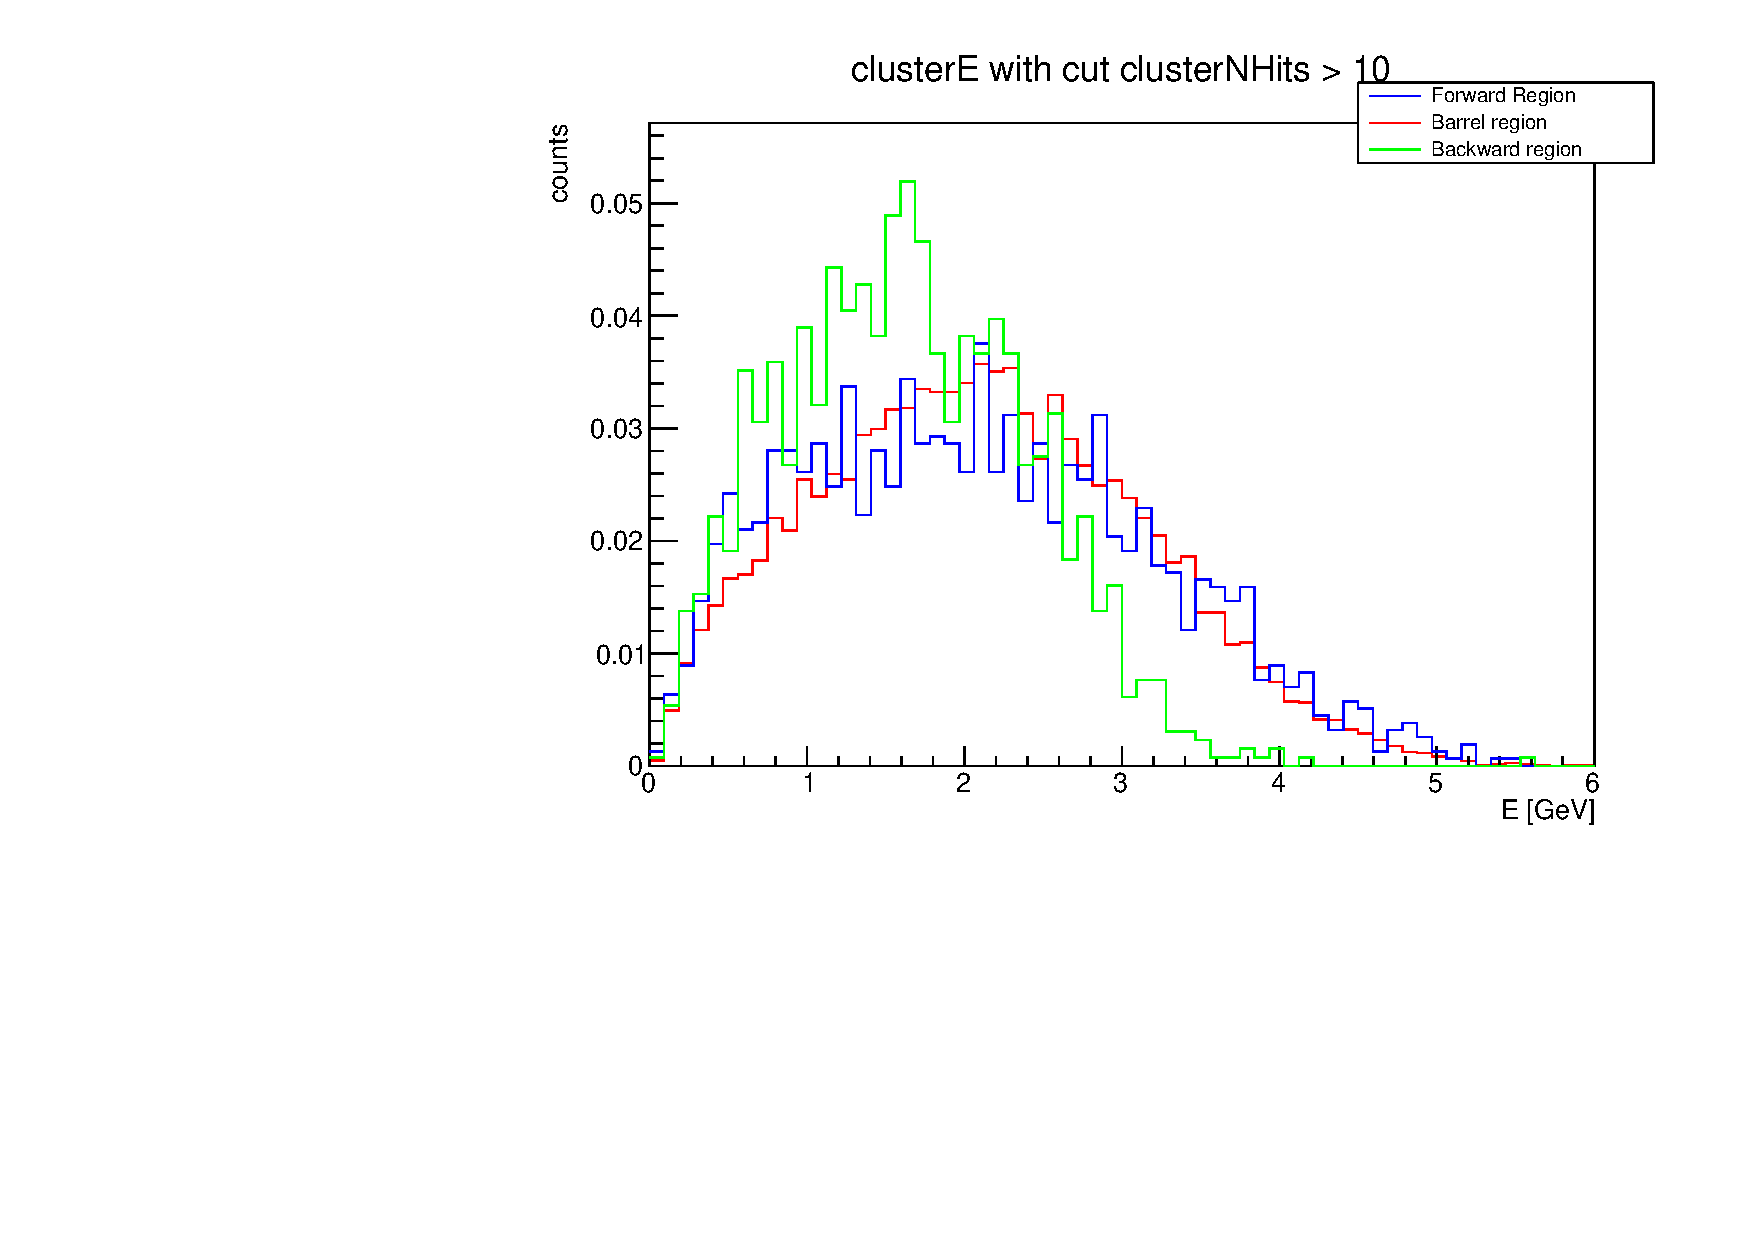
\includegraphics[width=0.49\textwidth]{nbar_MC/images/clusterE_nog_region.pdf}
    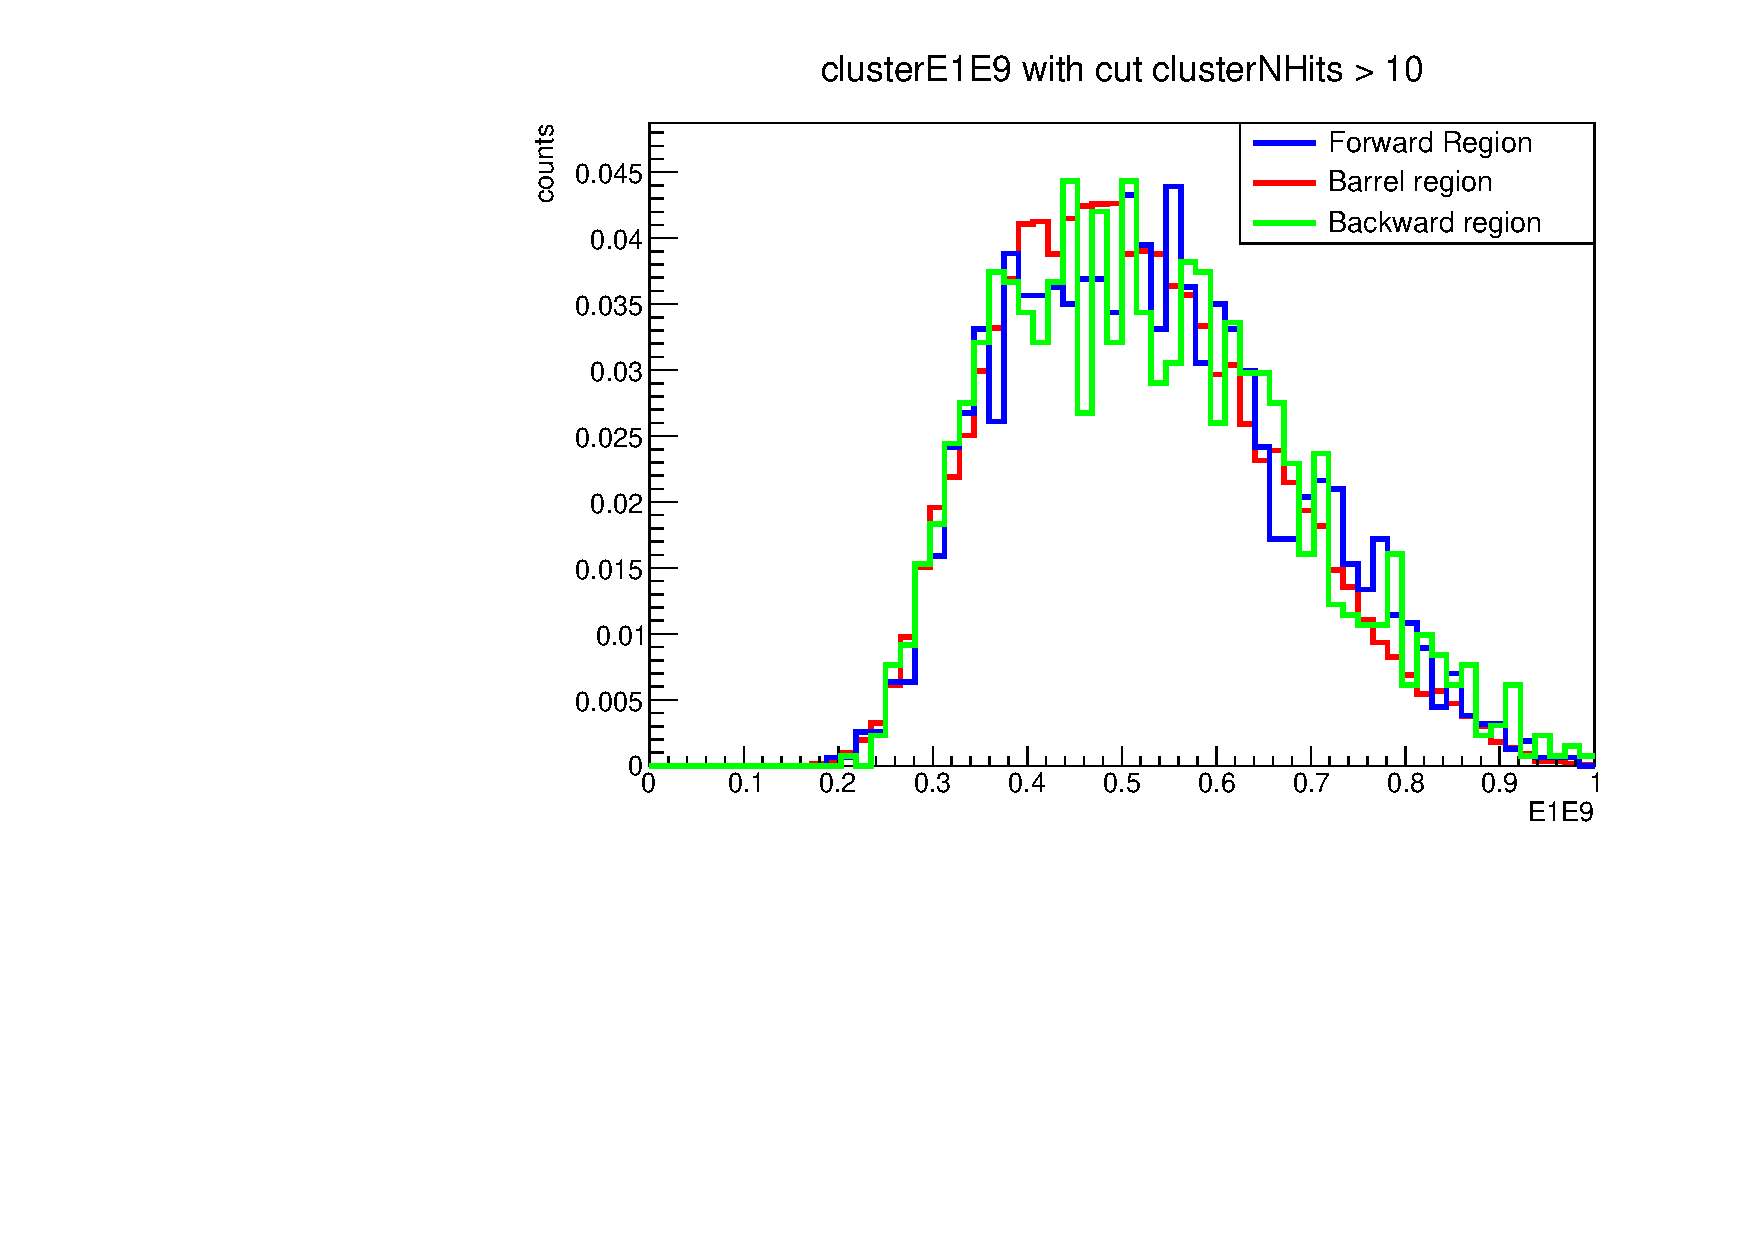
\includegraphics[width=0.49\textwidth]{nbar_MC/images/clusterE1E9_nog_region.pdf}
    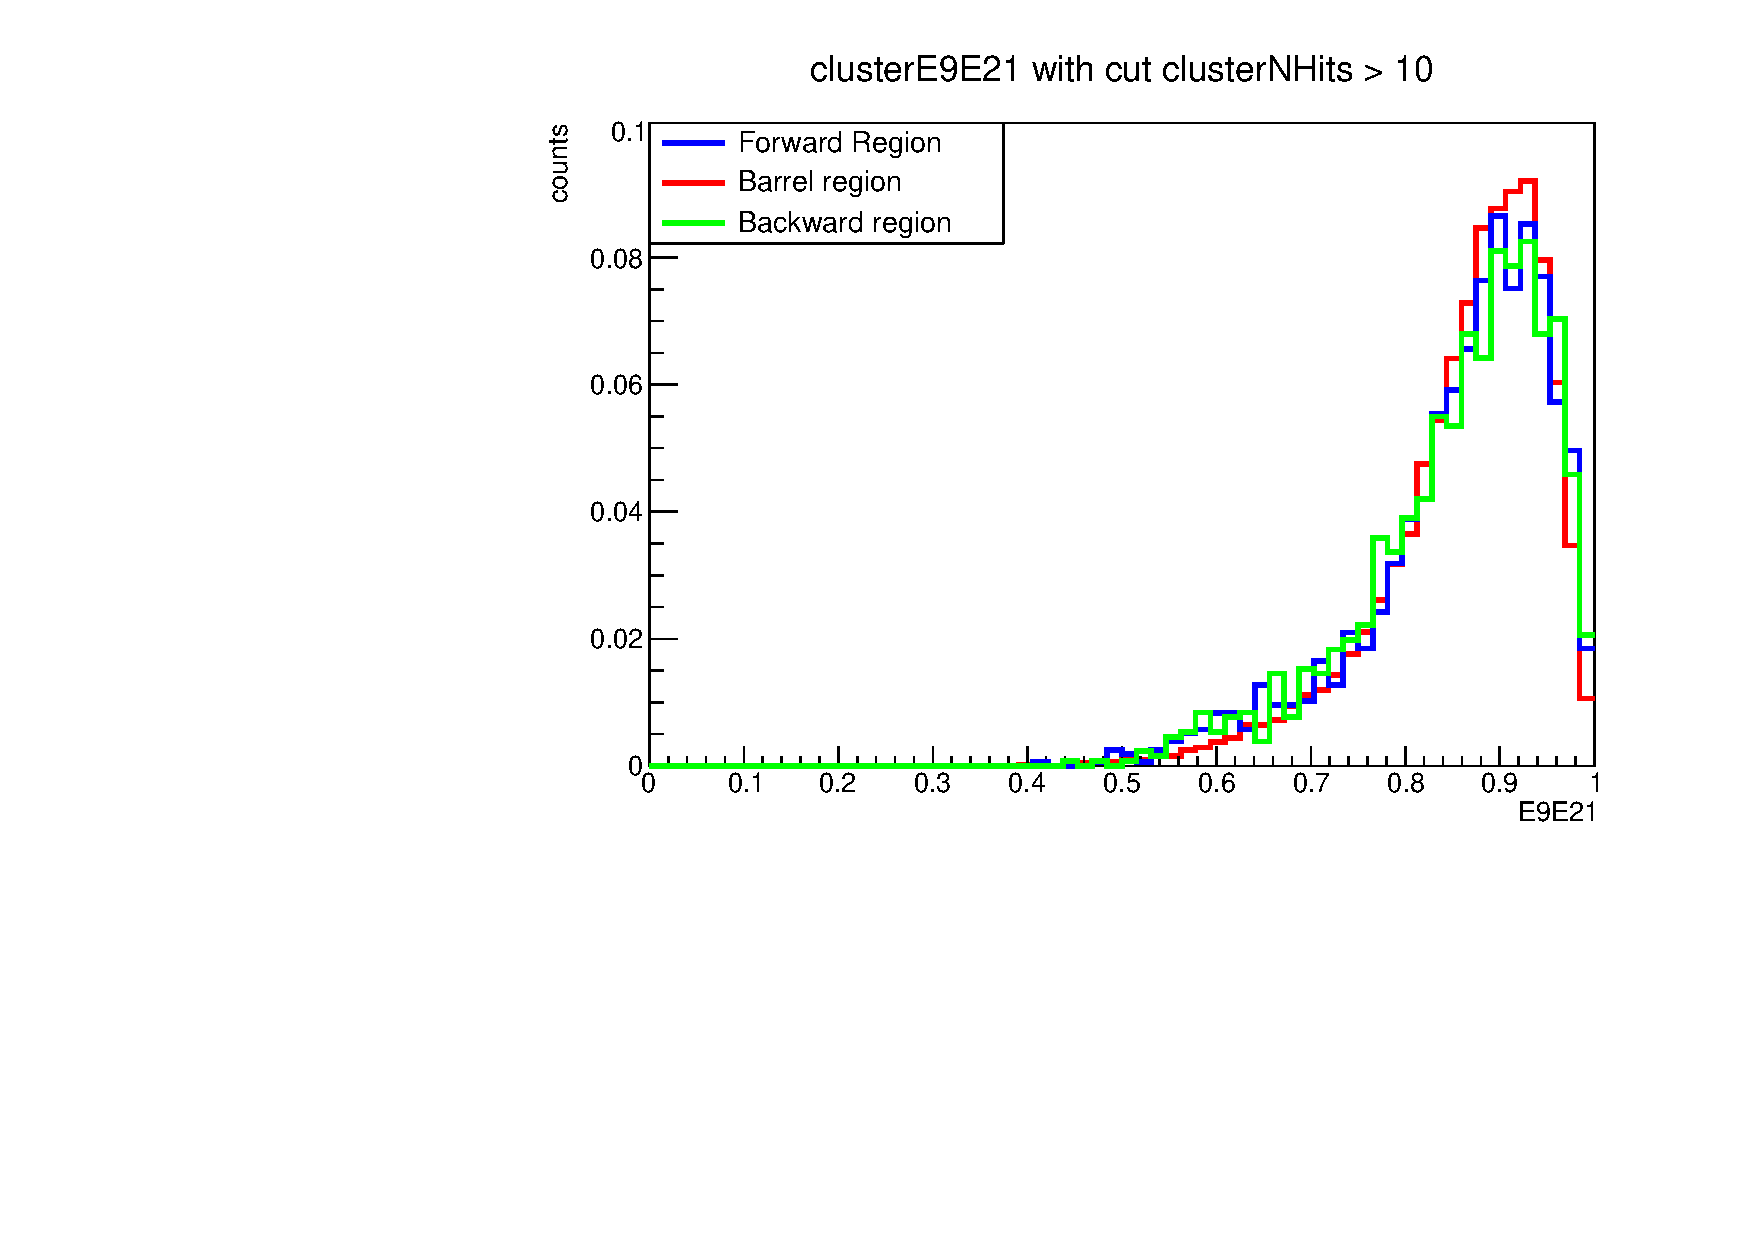
\includegraphics[width=0.49\textwidth]{nbar_MC/images/clusterE9E21_nog_region.pdf}
    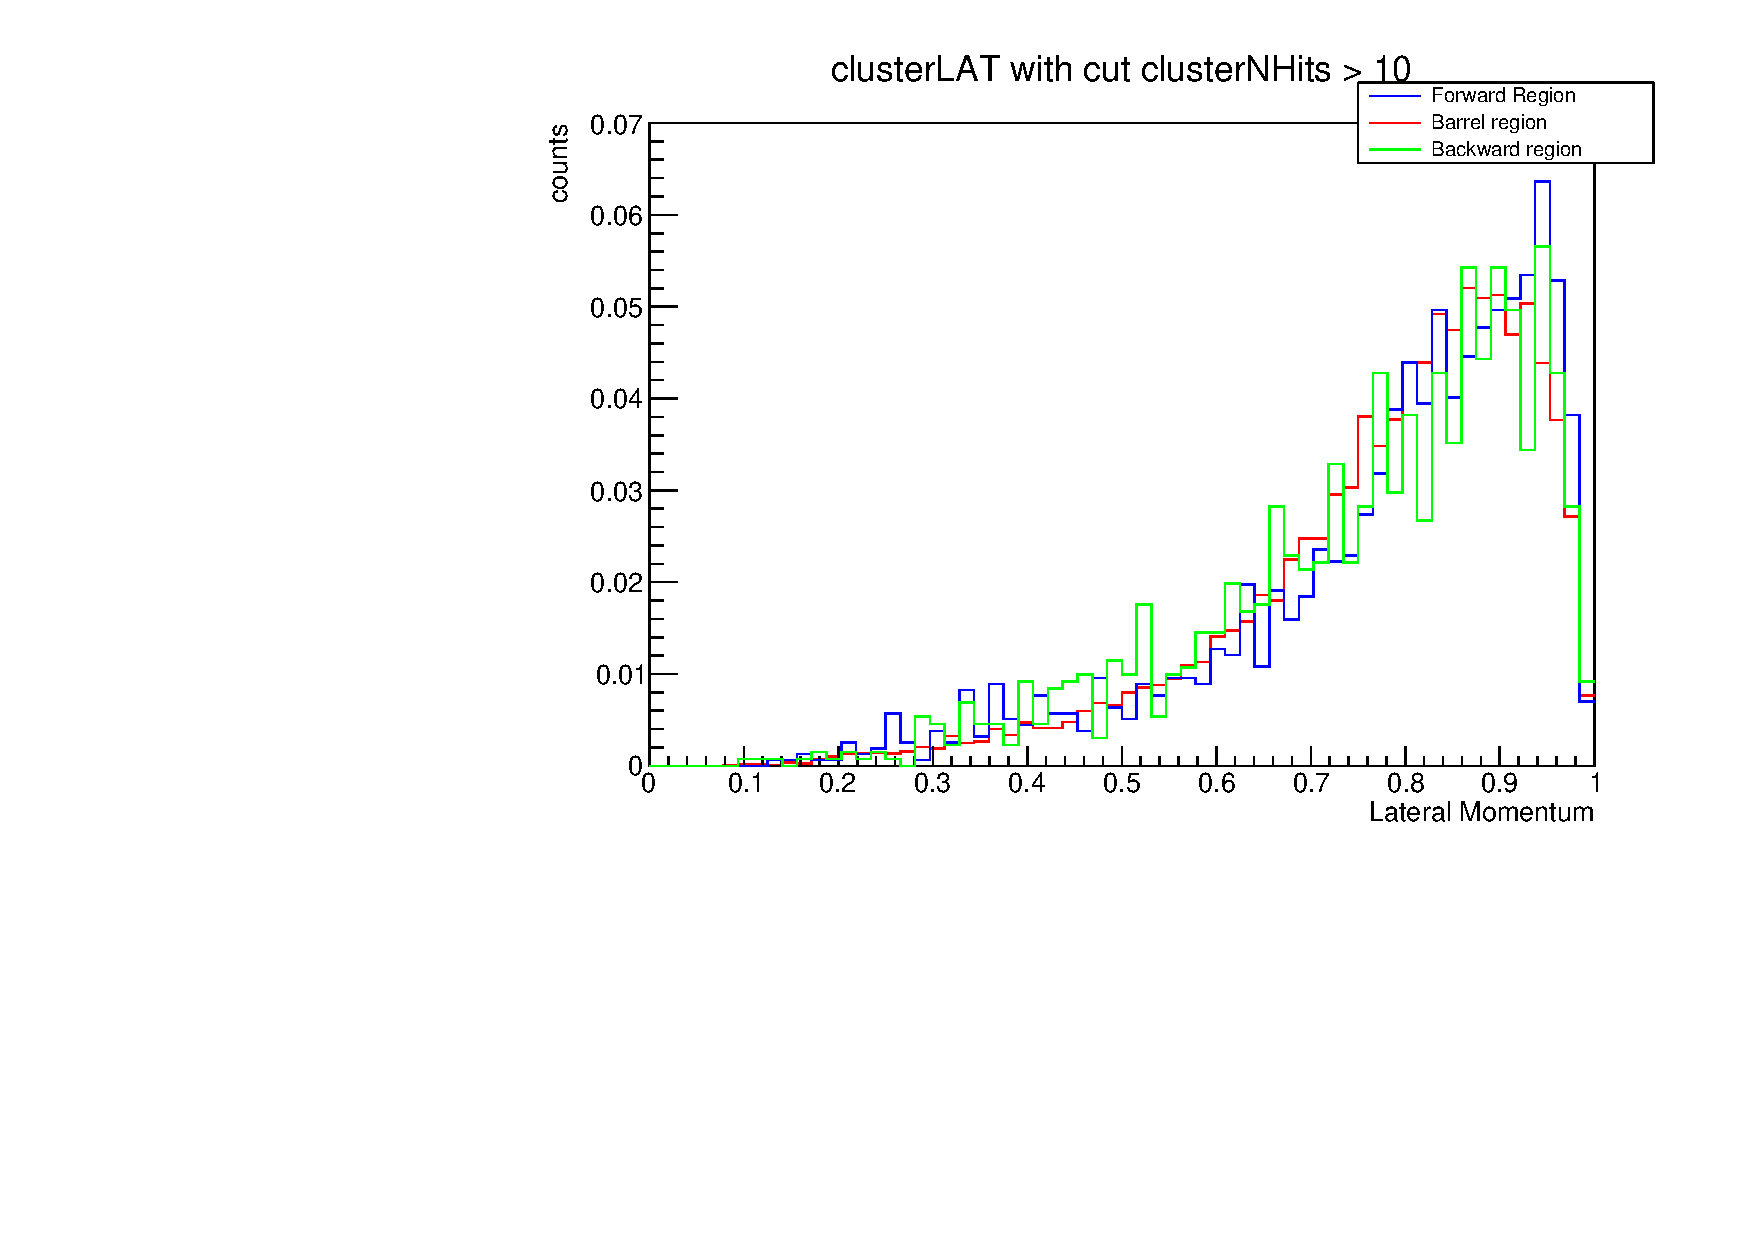
\includegraphics[width=0.49\textwidth]{nbar_MC/images/clusterLAT_nog_region.pdf}
    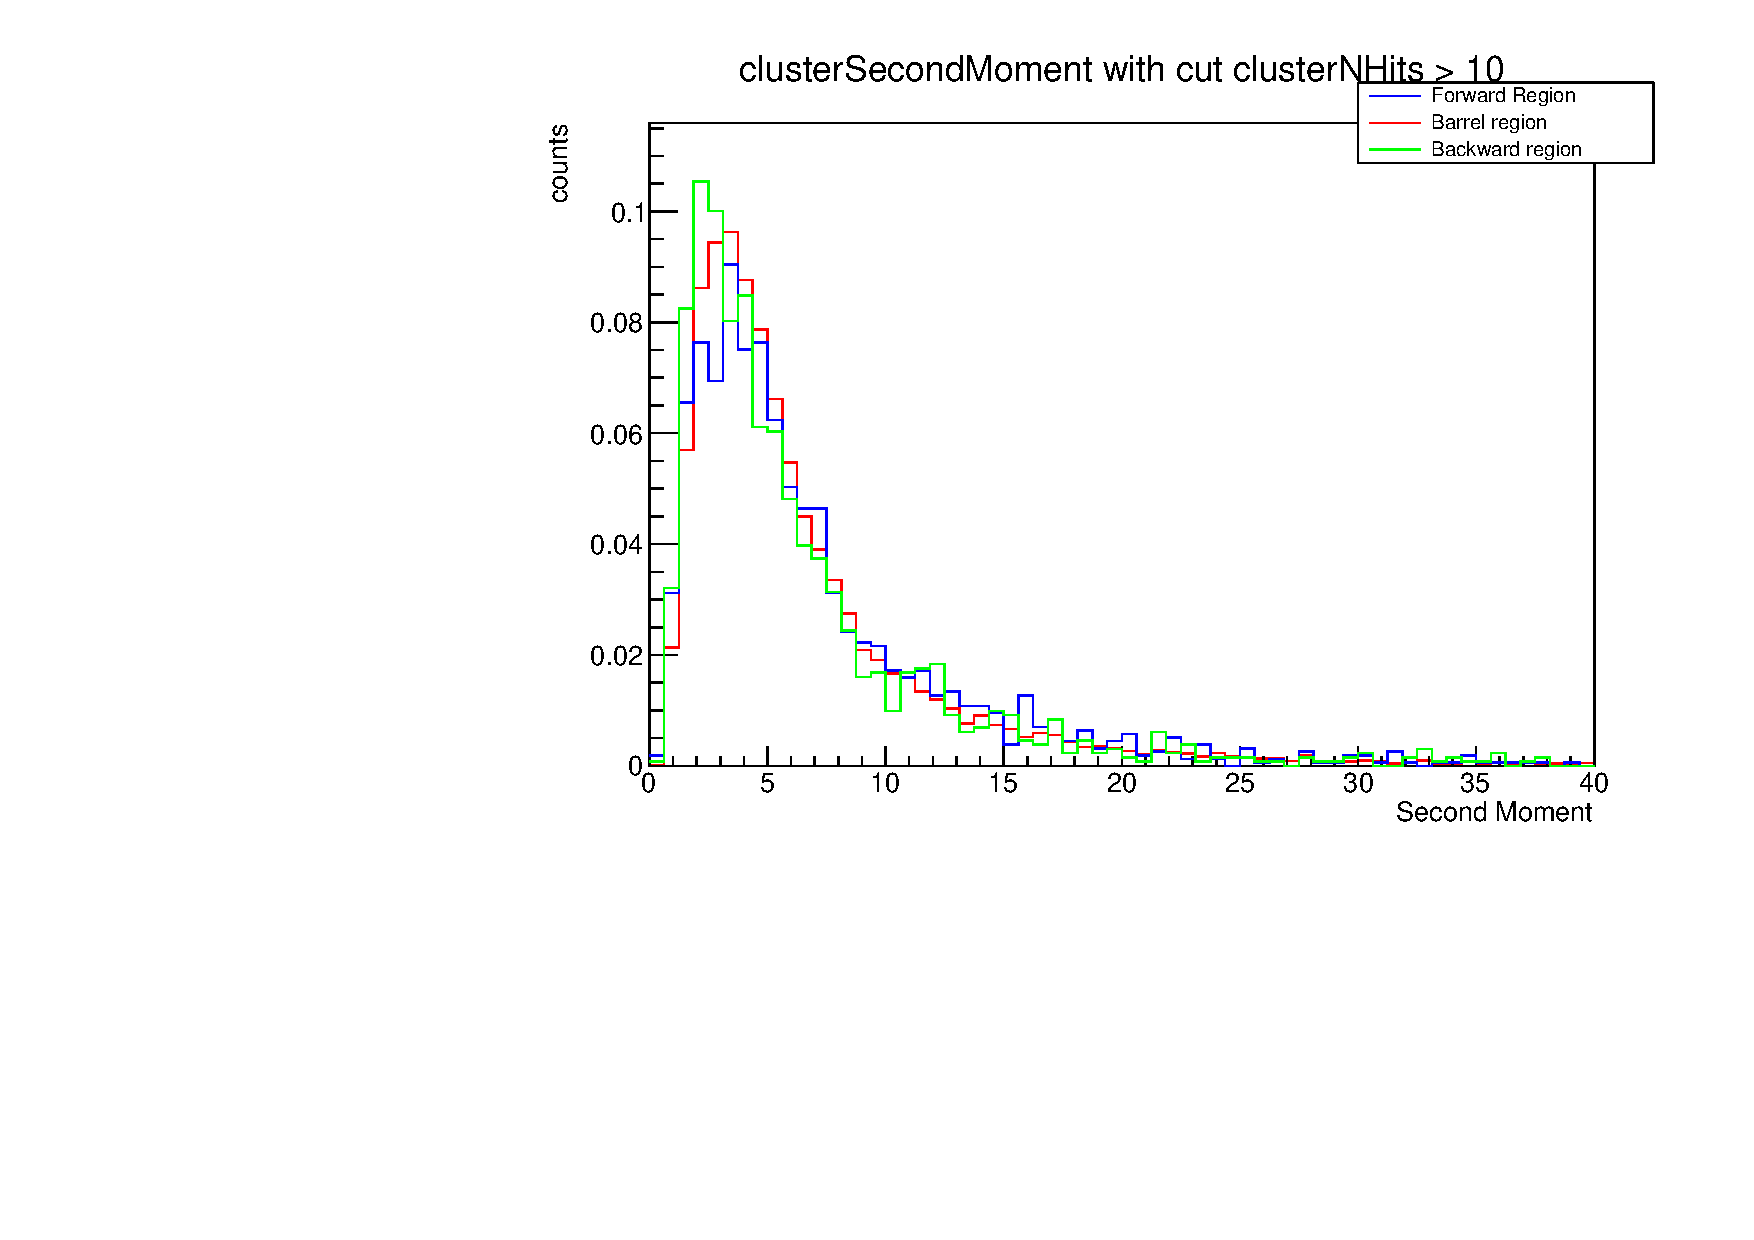
\includegraphics[width=0.49\textwidth]{nbar_MC/images/clusterSecondMoment_nog_region.pdf}
    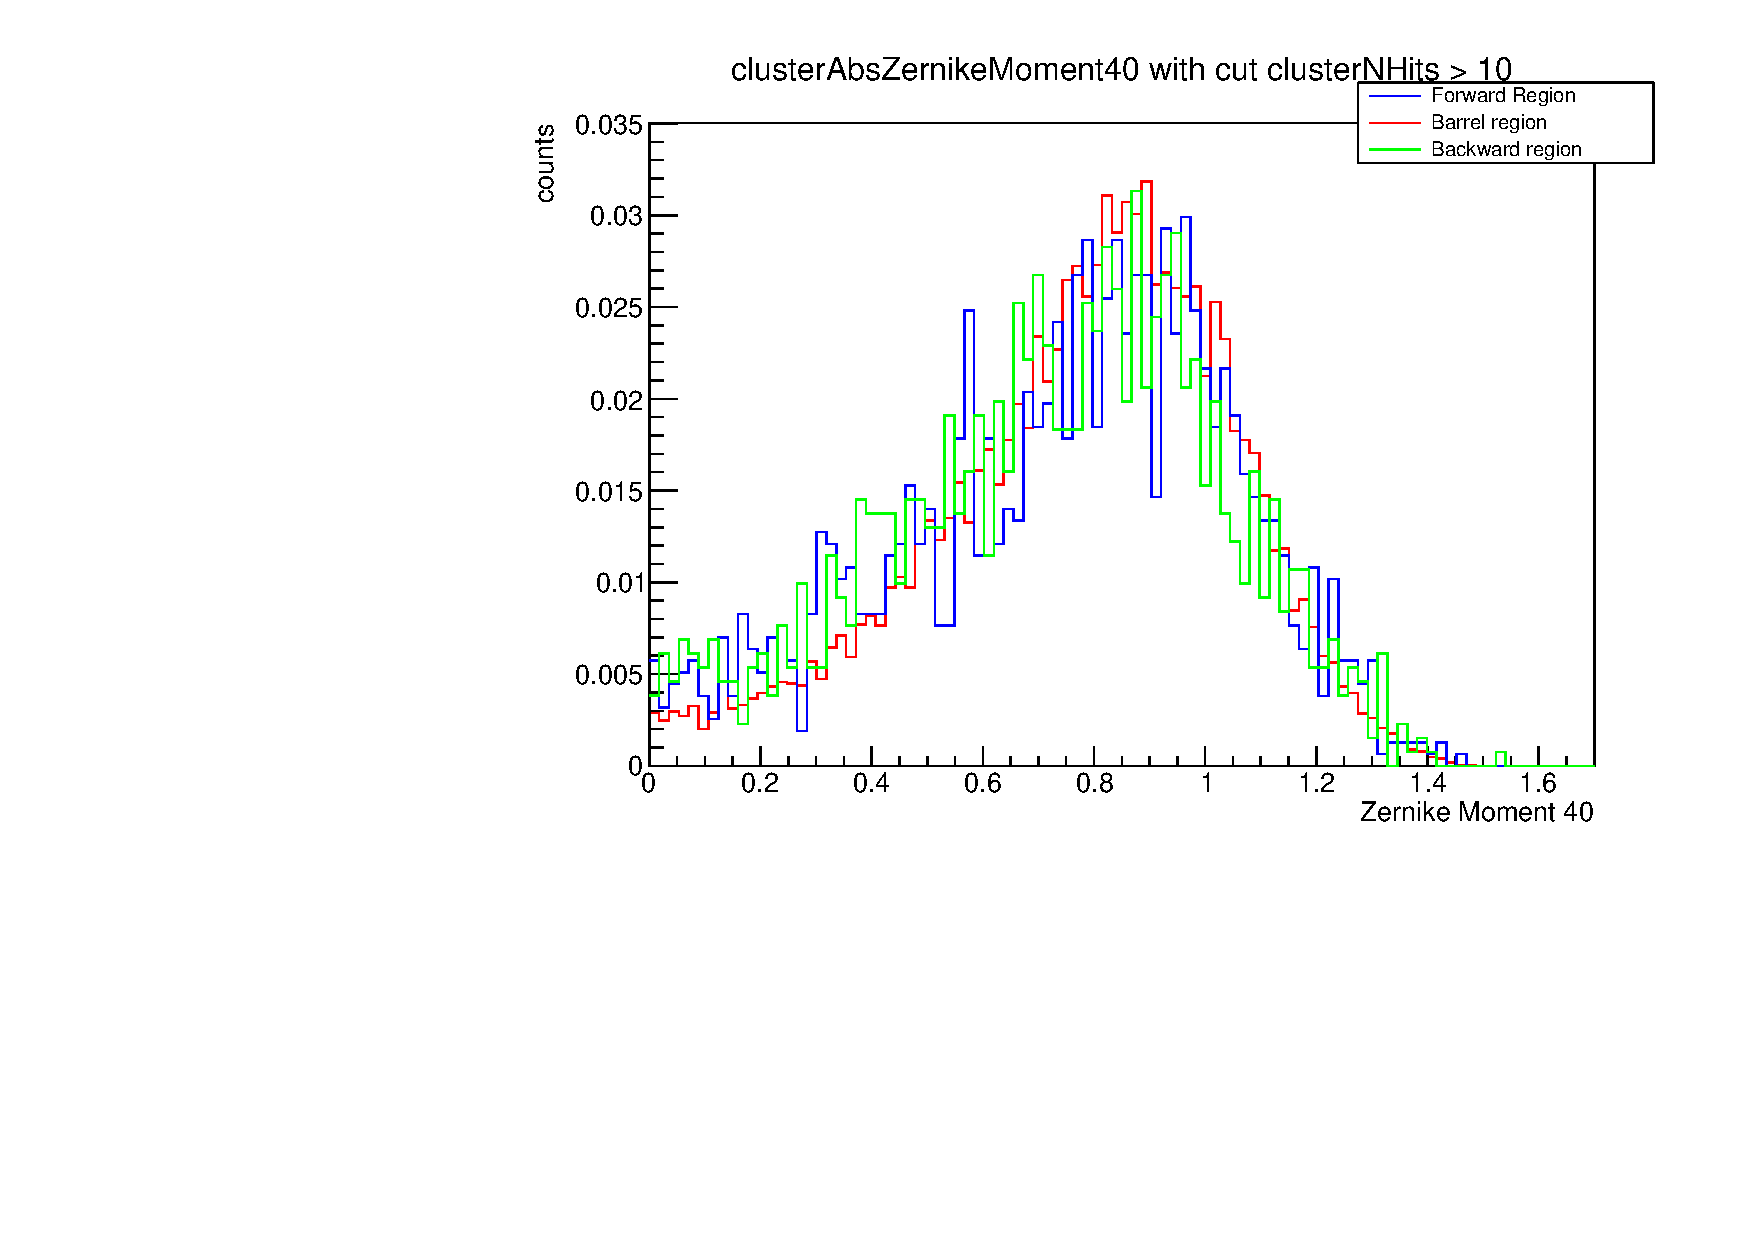
\includegraphics[width=0.49\textwidth]{nbar_MC/images/clusterAbsZernikeMoment40_nog_region.pdf}
    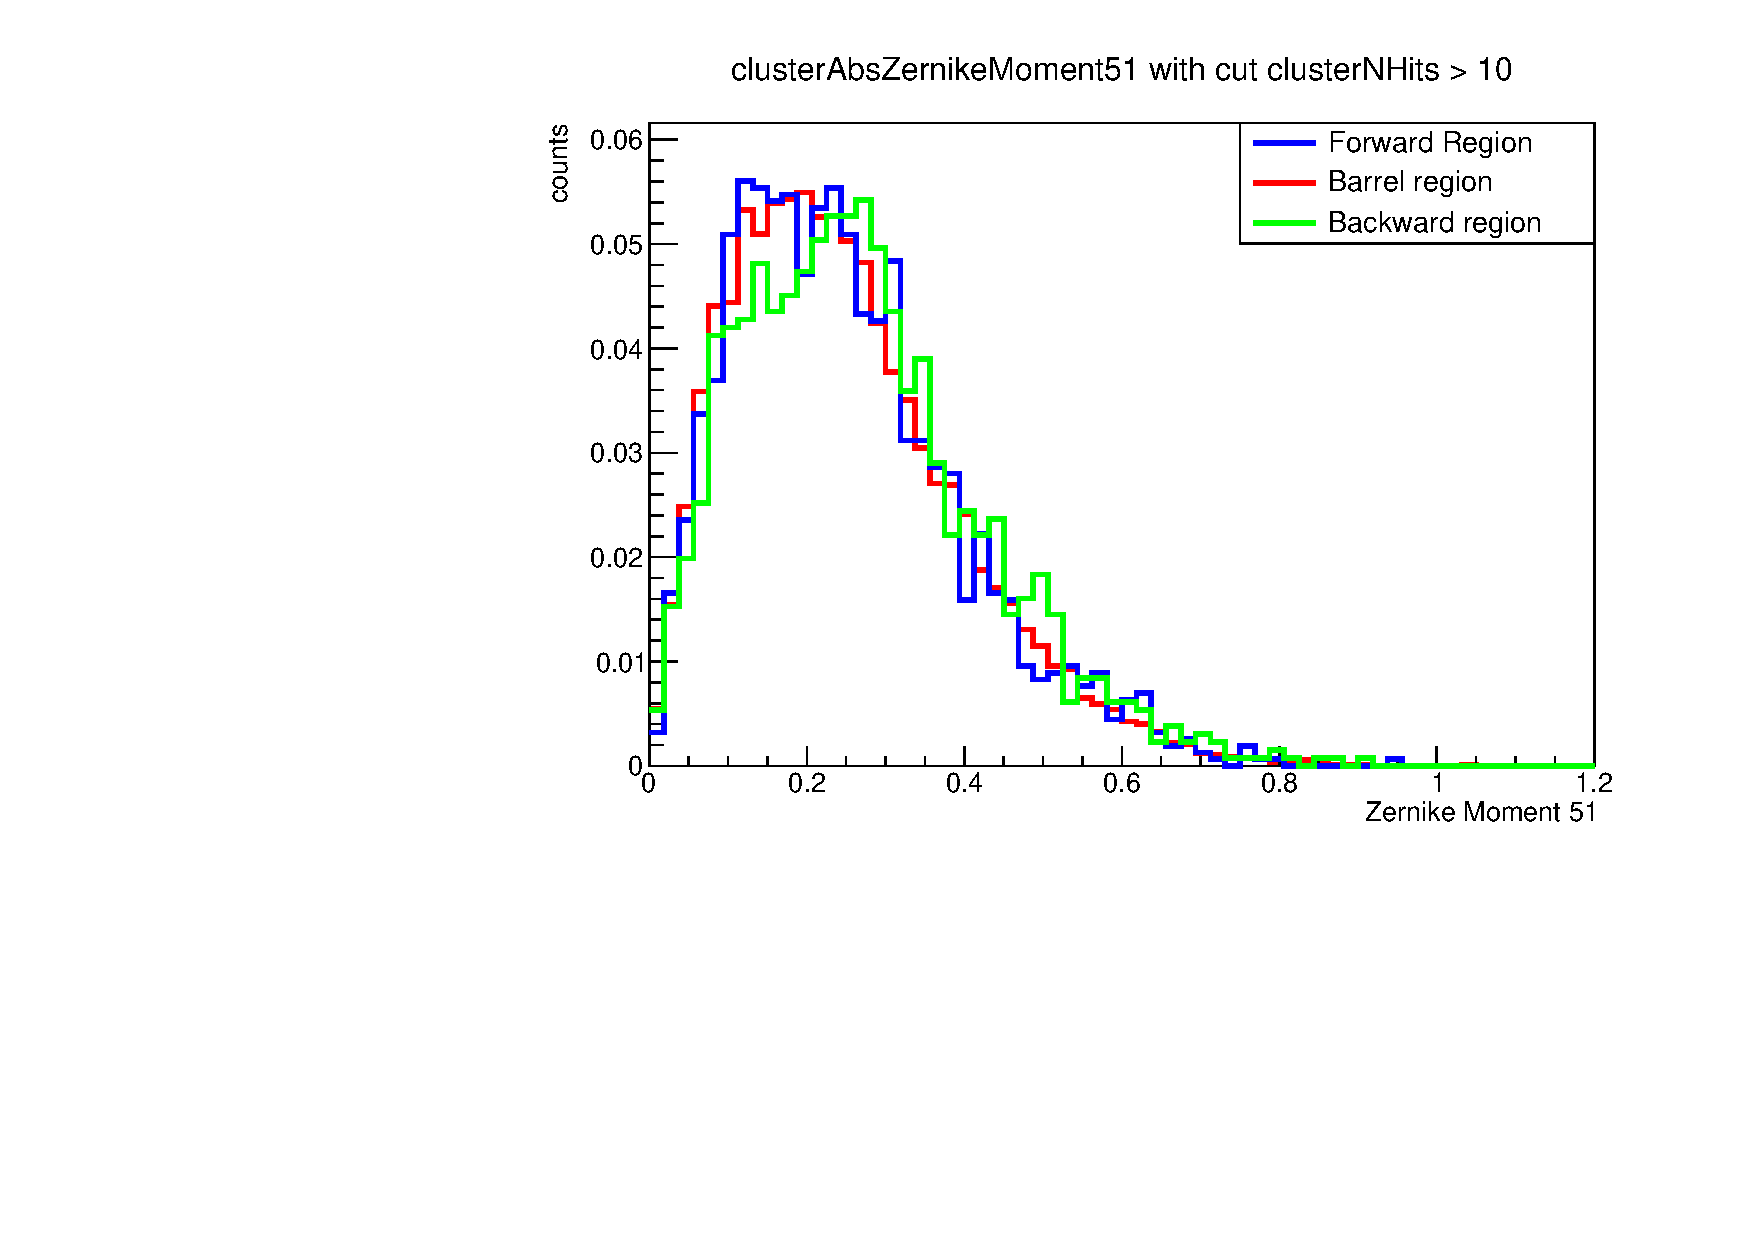
\includegraphics[width=0.49\textwidth]{nbar_MC/images/clusterAbsZernikeMoment51_nog_region.pdf}
    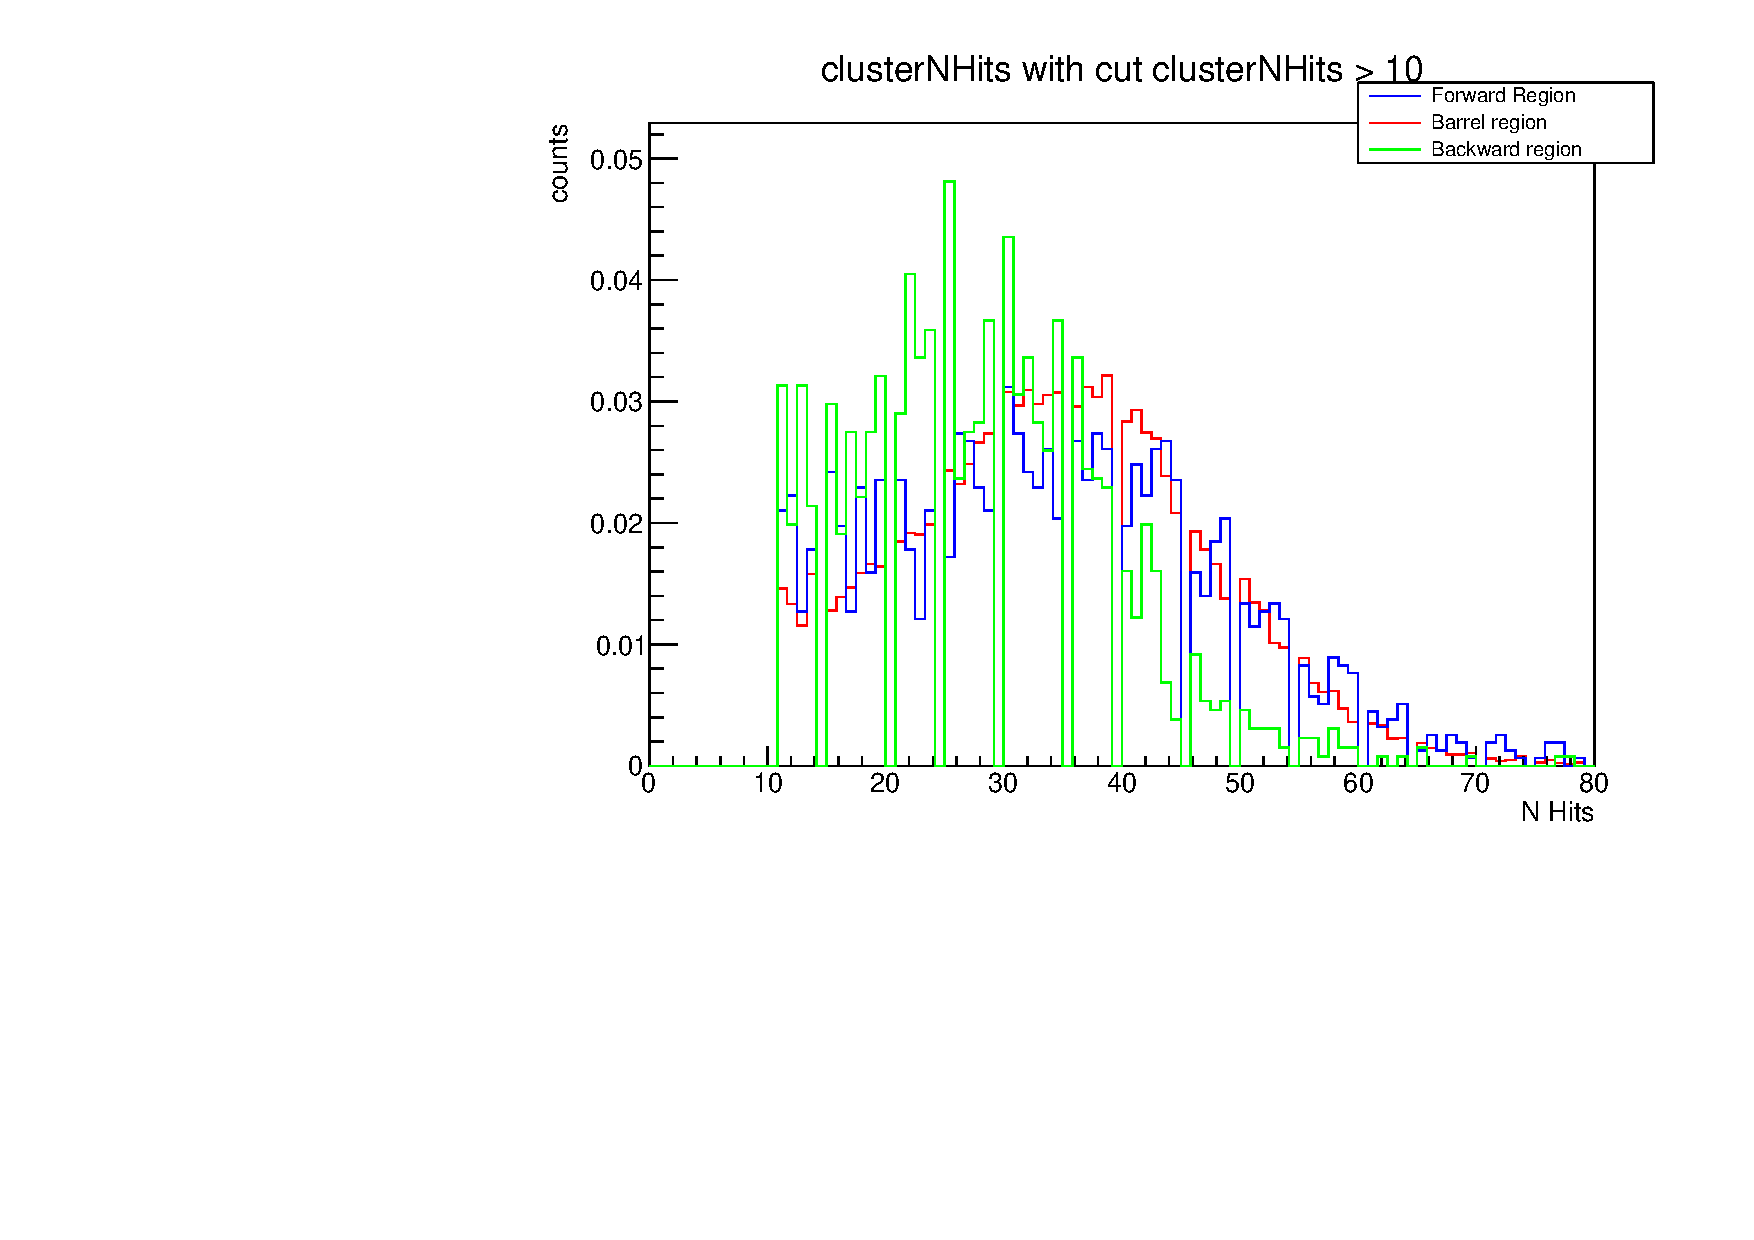
\includegraphics[width=0.49\textwidth]{nbar_MC/images/clusterNHits_nog_region.pdf}
   
     \caption{Comparison of reconstructed cluster variables for all $\bar{n}$ candidates in different ECL regions. The distributions are normalized to unit value}
      \label{fig:cluster_region}
\end{figure}

\subsection{Summary of Signal Channel Analysis}
The channel $e^+ \ + \  e^- \rightarrow p \ + \ \pi^- \ + \ \bar{n} $ has been studied, with both ISR and NO ISR emission. 
$\\$
$\\$
The recoil system $p\pi^-(\gamma_{ISR})$ is correctly reconstructed by the analysis, as evidenced by the peak above the anti-neutron mass in the recoil mass distribution. Furthermore, the kinematic distributions ($p$ and $\theta$) of the recoil system are consistent with those of generator-level $\bar{n}$ candidates, in both ISR and NO ISR cases. At reconstructed level, good agreement is observed in the $\theta$ distribution, while the reconstructed $\bar{n}$ candidate momentum shows underestimation and poor resolution compared to the recoil system momentum, as observed in correlations and residuals distributions. Furthermore, a low-momentum value structure is observed in reconstructed and generated momentum of $\bar{n}$ candidates compared to the recoil system momentum.
$\\$
$\\$
Therefore, energy loss occurs within ECL clusters, suggesting leakage processes such as cluster split-off and/or pre-showering effects. Ancestor studies reveal that photons related to $\bar{n}$ particles are often misidentified as main $\bar{n}$ candidates, accounting for the low-momentum structure observed. In fact, the ancestors momentum can be partially recovered when good Monte Carlo associations occur, showing good agreement with the recoil system momentum as well. A study of $\bar{n}$ production reveals that candidates with $\bar{n}$ ancestors are generated far from the IP, before the ECL (pre-showering) and within the ECL (cluster split-off).
$\\$
$\\$
Furthermore, a one-constraint (1C) Kinematic Fit was tested, revealing no significant improvement in the reconstructed recoil momentum and confirming that the recoil system was already optimally reconstructed by the analysis. 
$\\$
$\\$
Eventually, the reconstructed cluster variables associated with $\bar{n}$ candidates -such as cluster energy, lateral momentum, Zernike moments, etc.- were studied in the Monte Carlo signal sample. Similar structures to those observed in the momentum distributions were identified, particularly in the cluster energy and number of hits distributions.Therefore, ancestor studies confirm the momentum distribution observations: sub-clusters from secondary particles with $\bar{n}$ ancestry produce small-sized, low-energy structures in the cluster distributions.
$\\$
$\\$
In particular, a cut on the cluster number of hits yields reconstructed cluster variables closer to those expected from Monte Carlo $\bar{n}$ candidate selection, in both ISR and NO ISR cases.


